\documentclass[11pt,a4paper]{article}

\usepackage{amsfonts,amssymb,amsmath}
\usepackage[margin=1in]{geometry}
\usepackage[none]{hyphenat}
\usepackage{graphicx}
\usepackage{fancyhdr}
\usepackage{float}
\usepackage{color}
\usepackage{xcolor}
\usepackage{tikz}
\usepackage{esint}
\usepackage[nottoc,notlot,notlof]{tocbibind}

\usetikzlibrary{quotes,angles,graphs,patterns,arrows.meta,arrows,shapes,trees,bending,fadings}
\usetikzlibrary{decorations.pathmorphing}
\usetikzlibrary{decorations.markings}

\parindent 0ex
\setlength{\parskip}{0.55\baselineskip}
% Displays carry their own skips; with a non-zero \parskip on top of them,
% consecutive displays drift apart. Tighten them so a derivation reads as one
% argument rather than as a column of disconnected formulae. This document is
% mostly derivations, so it matters more here than in any other course.
\setlength{\abovedisplayskip}{0.5\baselineskip}
\setlength{\belowdisplayskip}{0.5\baselineskip}
\setlength{\abovedisplayshortskip}{0.25\baselineskip}
\setlength{\belowdisplayshortskip}{0.25\baselineskip}

\pagestyle{fancy}
\fancyfoot[C]{\thepage}
\fancyhead{}
\fancyhead[R]{\rightmark}

% Theorem environments. The source declared none: every definition, example,
% theorem and solution was set as bold text, so nothing was numbered by LaTeX,
% nothing could be cross-referenced, and inserting an example meant renumbering
% the rest of the subsection by hand.
\usepackage{amsthm}
\theoremstyle{definition}
% One shared counter running section.subsection.n, as in the other courses here,
% so a reader can find "Example 1.2.4" without knowing which kind of result it
% is. Notes and remarks stay unnumbered: they interrupt rather than advance.
\newtheorem{thm}{Theorem}[subsection]
\newtheorem{defn}[thm]{Definition}
\newtheorem{exa}[thm]{Example}
\newtheorem{prop}[thm]{Proposition}
\newtheorem{coro}[thm]{Corollary}
\newtheorem{lem}[thm]{Lemma}
\newtheorem{result}[thm]{Result}
\newtheorem{exe}[thm]{Exercise}
\newtheorem*{note}{Note}
\newtheorem*{remark}{Remark}
\newtheorem{problemx}{Problem}[subsection]
\newenvironment{problem}{\begin{problemx}}{\end{problemx}}
\newenvironment{solution}
  {\renewcommand{\qedsymbol}{}\begin{proof}[\textit{Solution}.]}
  {\end{proof}}
\usepackage{enumitem}
% A heading that is legal inside a theorem body, a list or a float, where
% \subsubsection is not. Same weight as \subsubsection* so the two read alike.
\newcommand{\subhead}[1]{%
  \par\medskip\noindent\textbf{#1}\par\nobreak\smallskip}

\begin{document}

% Title page depersonalised for the web, as with every other course here: no
% university crest, no author, no year. The identity kept below is the polar
% equation of a conic -- one equation that yields the circle, the parabola, the
% ellipse and the hyperbola as the eccentricity varies, which is the unifying
% idea the first section is built around.
\begin{titlepage}
\begin{center}
\vspace*{3cm}
{\Huge\bfseries Analytic Geometry\\[0.35cm] and Calculus}\\[1.2cm]
{\large Lecture Notes}\\[2.5cm]
\line(1,0){300}\\[1.5cm]
$$r=\frac{ep}{1+e\cos\theta}$$
\end{center}
\end{titlepage}

\tableofcontents
\thispagestyle{empty}
\clearpage
\setcounter{page}{1}

\section{Analytic Geometry}

Analytic geometry studies geometric objects through the equations their points
satisfy. The gain is that questions about shape become questions about algebra:
the property that defines a curve is written as a relation between coordinates,
and the relation can then be manipulated by ordinary calculation.

This section works that idea through the conic sections --- the circle,
parabola, ellipse and hyperbola --- so called because each arises as the
intersection of a plane with a cone, the curve obtained depending only on how
the plane is tilted. Each is defined by a distance property, and in every case
the same three steps turn that property into an equation: write the distances
with the distance formula, clear the square roots by squaring, and simplify.

Two later ideas unify what the derivations produce separately. The eccentricity
$e$ is a single number distinguishing the curves, so that the four cases become
one family; and in polar coordinates that family collapses into the single
equation $r = \dfrac{ep}{1 + e\cos\theta}$. The section closes with the change
of axes --- translation and rotation --- needed to recognise a conic whose axes
are not those of the coordinate system.


\subsection{Conic Sections}
Conic sections, as the name implies, are the curves obtained by cutting a cone with a plane. Depending on the inclination of the cutting plane to the axis of the cone, the following curves occur

\begin{enumerate}
\item Circle 
\item Parabola
\item Ellipse
\item Hyperbola
\end{enumerate}

\subsection{Parabola}
A parabola is a locus of points $P$ which are equidistant from a fixed point (called the focus) and a fixed line (called the directrix).

% DIAGRAM 1

\begin{figure}[H]
\centering
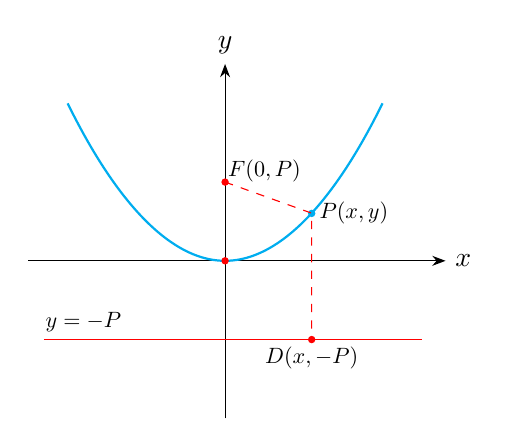
\begin{tikzpicture}[=>stealth]
\draw[-Stealth](-2.5,0)--(2.8,0)node[right]{$x$};
\draw[-Stealth](0,-2)--(0,2.5)node[above]{$y$};
\draw[thick,cyan](0,0)parabola(2,2);
\draw[thick,cyan](0,0)parabola(-2,2);
\draw[red](-2.3,-1)--(2.5,-1);
\draw(0,1)node[shape=circle,fill=red,scale=0.01cm]{}
(1.1,-1)node[shape=circle,fill=red,scale=0.01cm]{}
(0,0)node[shape=circle,fill=red,scale=0.01cm]{}
(1.1,0.602)node[shape=circle,fill=cyan,scale=0.01cm]{}
(1.1,0.602)node[right,scale=0.8]{$P(x,y)$}
(1.1,-1)node[below,scale=0.8]{$D(x,-P)$}
(0.5,0.9)node[above,scale=0.8]{$F(0,P)$}
(-1.8,-1)node[above,scale=0.8]{$y=-P$};
\draw[dashed,red](0,1)--(1.1,0.605)--(1.1,-1);
\end{tikzpicture}
\end{figure}

Let the focus be the point $F(0,P)$ , the vertex be the point $(0,0)$ and the directrix the line $y = -P$. If $P(x,y)$ lies on the parabola then $FP = PD$.

$$\implies \hspace{0.4cm} \sqrt{(x- 0)^2 + (y  - P)^2}  = \sqrt{(x - x)^2 + (y-(-p))^2}$$

$$\implies \hspace{0.5cm} \Big(\sqrt{x^2 + (y - P)^2}\Big)^2 = (y+P)^2$$

$$\implies\hspace{0.5cm} x^2 + y^2 - 2Py + P^2 = y^2 + 2Py + P^2$$

$$\boxed{x^2 = 4Py}$$

$\implies\hspace{0.3cm} x^2 = 4Py\hspace{0.3cm}$ which is the standard equation of a parabola whose focus $F(0,P)$ and directrix $y = -P$.


The standard equation of a parabola which opens downward with focus $F(0, -P)$ and directrix $y = P$ is given by \hspace{0.2cm}$\boxed{x^2 = -4Py}$

% DIAGRAM 2

\begin{figure}[H]
\centering
\begin{tikzpicture}[=>stealth]
\draw[-Stealth](-2.8,0)--(2.5,0)node[right]{$x$};
\draw[-Stealth](0,-2.5)--(0,2)node[above]{$y$};
\draw[thick,cyan](0,0)parabola(-2,-2);
\draw[thick,cyan](0,0)parabola(2,-2);
\draw[red](-2.5,1)--(2.5,1);
\draw[dashed,red](0,-1)--(-1.1,-0.602)--(-1.1,1);
\draw(0,0)node[shape=circle,fill=red,scale=0.01cm]{}
(0,-1)node[shape=circle,fill=red,scale=0.01cm]{}
(-1.1,-0.602)node[shape=circle,fill=cyan,scale=0.01cm]{}
(-1.1,1)node[shape=circle,fill=red,scale=0.01cm]{}
(-1.1,1)node[above,scale=0.8]{$D$}
(-1.1,-0.602)node[left,scale=0.8]{$P$}
(0,-1)node[right,scale=0.8]{$F(0,-P)$}
(1.6,1)node[above,scale=0.8]{$y=P$};
\end{tikzpicture}
\end{figure}

\begin{exe}


Derive the equation $x^2 = -4Py$.\


$\star$ The standard equation of a parabola which opens to the right along the $x-$axis with focus $F(0,P)$ and directrix on the line $x = -P$ is given by \hspace{0.2cm}$\boxed{y^2 = 4Px}$

% DIAGRAM 3

\begin{figure}[H]
\centering
\begin{tikzpicture}[=>stealth]
\draw[-Stealth](-2.5,0)--(3.5,0)node[right]{$x$};
\draw[-Stealth](0,-3)--(0,3)node[above]{$y$};
\draw[smooth,thick,cyan,domain=0:2,variable=\x]plot(\x,{sqrt(2*\x)});
\draw[smooth,thick,cyan,domain=0:2,variable=\x]plot(\x,{-sqrt(2*\x)});
\draw[red](-1,-2.5)--(-1,2.5);
\draw(0,0)node[shape=circle,fill=red,scale=0.01cm]{}
(1.2,0)node[shape=circle,fill=red,scale=0.01cm]{}
(1,1.4)node[shape=circle,fill=cyan,scale=0.01cm]{}
(-1,1.4)node[shape=circle,fill=red,scale=0.01cm]{}
(-1,1.4)node[left,scale=0.8]{$D$}
(1,1.3)node[right,scale=0.8]{$P(x,y)$}
(1.2,0)node[below,scale=0.8]{$F(P,0)$}
(-1,-2.5)node[below]{$x=-p$};
\draw[dashed,red](1.2,0)--(1,1.4);
\draw[dashed,red](1,1.4)--(-1,1.4);
\end{tikzpicture}
\end{figure}

The standard equation of the parabola which open to the left with focus $F(-P,0)$ and directrix on the line $x = P$ is given by \hspace{0.2cm}$\boxed{ y^2 = - 4Px}$
\end{exe}


\begin{exe}


Derive the equations $y^2 = 4Px$ and $y^2= -4Px$.
\end{exe}


\subsection{Ellipse}
An ellipse is a locus of points $P$ such that the sum of the distance from $P$ to two fixed points $F$ and $F'$  (called the foci) is a constant.

% DIAGRAM 4

\begin{figure}[H]
\centering
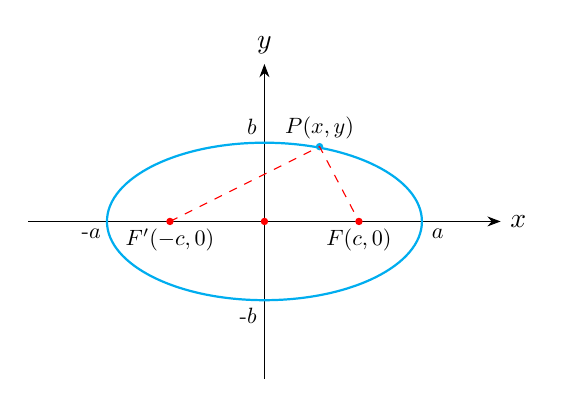
\begin{tikzpicture}[=>stealth]
\draw[-Stealth](-3,0)--(3,0)node[right]{$x$};
\draw[-Stealth](0,-2)--(0,2)node[above]{$y$};
\draw[thick,cyan](0,0)ellipse[x radius=2,y radius=1];
\draw(0,0)node[shape=circle, fill=red, scale=0.01cm]{}
(-1.2,0)node[shape=circle,fill=red,scale=0.01cm]{}
(1.2,0)node[shape=circle,fill=red,scale=0.01cm]{}
(0.7,0.95)node[shape=circle,fill=cyan,scale=0.01cm]{}
(-1.2,0)node[below,scale=0.8]{$F'(-c,0)$}
(1.2,0)node[below,scale=0.8]{$F(c,0)$}
(0.7,0.95)node[above,scale=0.8]{$P(x,y)$}
(0,-1.2)node[left,scale=0.8]{-$b$}
(0,1.2)node[left,scale=0.8]{$b$}
(2.2,0)node[below,scale=0.8]{$a$}
(-2.2,0)node[below,scale=0.8]{-$a$};
\draw[dashed,red](-1.2,0)--(0.7,0.95)--(1.2,0);
\end{tikzpicture}
\end{figure}

$$F'P + FP = 2a$$
From the diagram, the locus of $P$ is an ellipse if \hspace{0.2cm}$F'P + FP = 2a$. Thus,

$$ \sqrt{(x + c)^2 + ( y -0)^2} + \sqrt{(x-c)^2 + (y-0)^2} = 2a$$

$$\implies\hspace{0.5cm} \Big(\sqrt{(x + c)^2 + (y - 0)^2}\Big)^2 = \Big(2a - \sqrt{(x - c)^2 + (y - 0)^2}\Big)^2$$

$$\implies\hspace{0.5cm} x^2 +2cx + c^2 + y^2 = 4a^2 - 4a\sqrt{(x- c)^2 + y^2} + (x^2 -2cx + c^2 +y^2)$$

$$\implies\hspace{0.5cm} \frac{4a\sqrt{(x - c)^2 + y^2}}{4} = \frac{4a^2}{4} - \frac{4cx}{4}$$

$$\implies\hspace{0.5cm} \Big(a\sqrt{(x - c)^2 + y^2}\Big)^2 = \Big(a^2 - cx\Big)^2$$

$$\implies\hspace{0.5cm} a^2\Big[(x-c)^2 + y^2\Big] = a^4 -2a^2cx + c^2x^2$$

$$\implies\hspace{0.5cm} a^2x^2 - 2a^2cx + a^2c^2 + a^2y^2 = a^4 -2a^2cx + c^2x^2$$

$$\implies\hspace{0.5cm} a^2x^2 + a^2c^2 + a^2y^2 = a^4 + c^2x^2$$

$$\implies\hspace{0.5cm} a^2x^2 - c^2x^2 + a^2y^2 = a^4 - a^2c^2$$

$$\implies\hspace{0.5cm} x^2(a^2 -c^2) + a^2 y^2 = a^2 (a^2 - c^2)$$


Let $a^2 - c^2 = b^2$ thus we have $$b^2x^2 + a^2y^2 = a^2b^2$$

$$\boxed{\implies\hspace{0.5cm} \dfrac{x^2}{a^2} + \dfrac{y^2}{b^2} = 1}$$

which is the standard equation of an ellipse whose foci lie on the $x-$axis.


\begin{exa}


Write the standard equation of the ellipse with $F(1,0)$ $, \hspace{0.2cm} F(-1,0)$ and major axis 5.
\end{exa}


\begin{solution}


% DIAGRAM 5

\begin{figure}[H]
\centering
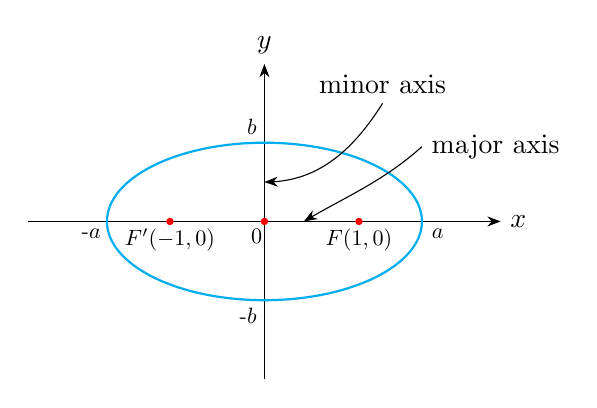
\begin{tikzpicture}[=>stealth]
\draw[-Stealth](-3,0)--(3,0)node[right]{$x$};
\draw[-Stealth](0,-2)--(0,2)node[above]{$y$};
\draw[thick,cyan](0,0)ellipse[x radius=2,y radius=1];
\draw(0,0)node[shape=circle, fill=red, scale=0.01cm]{}
(-1.2,0)node[shape=circle,fill=red,scale=0.01cm]{}
(1.2,0)node[shape=circle,fill=red,scale=0.01cm]{}
(-1.2,0)node[below,scale=0.8]{$F'(-1,0)$}
(1.2,0)node[below,scale=0.8]{$F(1,0)$}
(0,-1.2)node[left,scale=0.8]{-$b$}
(0,1.2)node[left,scale=0.8]{$b$}
(2.2,0)node[below,scale=0.8]{$a$}
(-2.2,0)node[below,scale=0.8]{-$a$}
(-0.1,0)node[below,scale=0.8]{$0$}
(1.5,1.5)node[above]{minor axis}
(2,0.95)node[right]{major axis};
\draw[-Stealth](1.5,1.5)..controls(1,0.7)and(0.5,0.5)..(0,0.5);
\draw[-Stealth](2,.95)..controls(1.5,0.5)and(1,0.3)..(0.5,0);
\end{tikzpicture}
\end{figure}

$$c = 1\hspace{0.2cm} ,\hspace{0.2cm} 2a= 5\hspace{0.3cm}\implies \hspace{0.3cm} a = \dfrac{5}{2}$$

$$b^2 = a^2 - c^2 \hspace{0.3cm} \implies \hspace{0.3cm} b^2 = \Big(\dfrac{5}{2}\Big)^2 - (1)^2 = \frac{21}{4}$$

Therefore, the equation of this ellipse is $$\dfrac{x^2}{25/4} + \dfrac{y^2}{21/4}= 1$$

$$\implies\hspace{0.5cm} \frac{4x^2}{25}+ \frac{4y^2}{21}=1$$


If an ellipse has its foci on the $y-$axis, then its standard equation is given by \hspace{0.2cm}$\boxed{\dfrac{x^2}{b^2} + \dfrac{y^2}{a^2}=1}$

% DIAGRAM 6

\begin{figure}[H]
\centering
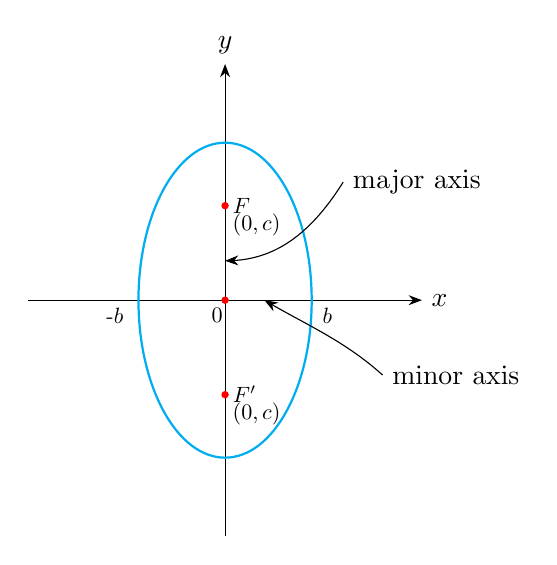
\begin{tikzpicture}[=>stealth]
\draw[-Stealth](-2.5,0)--(2.5,0)node[right]{$x$};
\draw[-Stealth](0,-3)--(0,3)node[above]{$y$};
\draw[thick,cyan](0,0)ellipse[x radius=1.1,y radius=2];
\draw(0,0)node[shape=circle, fill=red, scale=0.01cm]{}
(0,-1.2)node[shape=circle,fill=red,scale=0.01cm]{}
(0,1.2)node[shape=circle,fill=red,scale=0.01cm]{}
(-0.1,0)node[below,scale=0.8]{$0$}
(0,1.2)node[right,scale=0.8]{$F$}
(0.4,1.2)node[below,scale=0.8]{$(0,c)$}
(0,-1.2)node[right,scale=0.8]{$F'$}
(0.4,-1.2)node[below,scale=0.8]{$(0,c)$}
(1.5,1.5)node[right]{major axis}
(2,-0.95)node[right]{minor axis}
(-1.4,0)node[below,scale=0.8]{-$b$}
(1.3,0)node[below,scale=0.8]{$b$};
\draw[-Stealth](1.5,1.5)..controls(1,0.7)and(0.5,0.5)..(0,0.5);
\draw[-Stealth](2,-.95)..controls(1.5,-0.5)and(1,-0.3)..(0.5,0);
\end{tikzpicture}
\end{figure}
\end{solution}

\begin{exa}


An ellipse has its foci on the $y-$axis and its centre at origin. The distance between the foci is 6 and the major axis is of length 10. Find its equation.
\end{exa}


\begin{solution}


$\dfrac{2c}{2}=\dfrac{6}{2} \implies c = 3\hspace{0.3cm}$ Thus the foci are $F(0,3)$ and $F'(0,-3)$.

$$\frac{2a}{2} = \frac{10}{2}\hspace{0.3cm}\implies\hspace{0.3cm} a = 5$$

$$b^2 = a^2 - c^2 = 25 - 9 = 16$$

$$\implies\hspace{0.5cm} \frac{x^2}{16} + \frac{y^2}{25} = 1$$\
\end{solution}

\subsection{Hyperbola}
A hyperbola is a locus of points $P$ such that the \emph{difference} of the
distances from $P$ to two fixed points $F$ and $F'$ (called the foci) is a
constant. It is the one conic listed at the start of this section that the
preceding pages have not yet treated, and the only change from the ellipse is
that a sum becomes a difference --- which is what turns a closed curve into two
separate branches.

% DIAGRAM 3a

\begin{figure}[H]
\centering
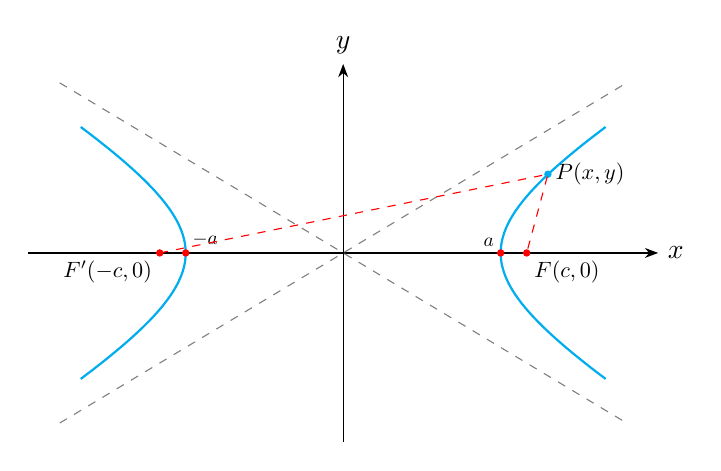
\begin{tikzpicture}[>=stealth]
\draw[-Stealth](-4,0)--(4,0)node[right]{$x$};
\draw[-Stealth](0,-2.4)--(0,2.4)node[above]{$y$};
\draw[dashed,gray,domain=-3.6:3.6,smooth,variable=\x] plot({\x},{0.6*\x});
\draw[dashed,gray,domain=-3.6:3.6,smooth,variable=\x] plot({\x},{-0.6*\x});
\draw[thick,cyan,domain=-1.6:1.6,smooth,variable=\y] plot({2*sqrt(1+(\y*\y)/1.44)},{\y});
\draw[thick,cyan,domain=-1.6:1.6,smooth,variable=\y] plot({-2*sqrt(1+(\y*\y)/1.44)},{\y});
\draw(2.33,0)node[shape=circle,fill=red,scale=0.01cm]{}
(-2.33,0)node[shape=circle,fill=red,scale=0.01cm]{}
(2.6,1.0)node[shape=circle,fill=cyan,scale=0.01cm]{}
(2.33,0)node[below right,scale=0.8]{$F(c,0)$}
(-2.33,0)node[below left,scale=0.8]{$F'(-c,0)$}
(2.6,1.0)node[right,scale=0.8]{$P(x,y)$}
(2,0)node[shape=circle,fill=red,scale=0.01cm]{}
(-2,0)node[shape=circle,fill=red,scale=0.01cm]{}
(2,0)node[above left,scale=0.7]{$a$}
(-2,0)node[above right,scale=0.7]{$-a$};
\draw[dashed,red](-2.33,0)--(2.6,1.0)--(2.33,0);
\end{tikzpicture}
\end{figure}

Let the foci be $F(c,0)$ and $F'(-c,0)$, and let the constant difference be
$2a$. If $P(x,y)$ lies on the hyperbola then
$$\left|F'P - FP\right| = 2a .$$
Taking the branch nearer $F$, so that $F'P - FP = 2a$,
$$\sqrt{(x + c)^2 + y^2} - \sqrt{(x - c)^2 + y^2} = 2a$$

$$\implies\hspace{0.5cm} \Big(\sqrt{(x + c)^2 + y^2}\Big)^2
= \Big(2a + \sqrt{(x - c)^2 + y^2}\Big)^2$$

$$\implies\hspace{0.5cm} x^2 + 2cx + c^2 + y^2
= 4a^2 + 4a\sqrt{(x - c)^2 + y^2} + \big(x^2 - 2cx + c^2 + y^2\big)$$

$$\implies\hspace{0.5cm} 4cx - 4a^2 = 4a\sqrt{(x - c)^2 + y^2}$$

$$\implies\hspace{0.5cm} \Big(cx - a^2\Big)^2 = \Big(a\sqrt{(x - c)^2 + y^2}\Big)^2$$

$$\implies\hspace{0.5cm} c^2x^2 - 2a^2cx + a^4
= a^2\Big[(x - c)^2 + y^2\Big]$$

$$\implies\hspace{0.5cm} c^2x^2 - 2a^2cx + a^4
= a^2x^2 - 2a^2cx + a^2c^2 + a^2y^2$$

$$\implies\hspace{0.5cm} c^2x^2 + a^4 = a^2x^2 + a^2c^2 + a^2y^2$$

$$\implies\hspace{0.5cm} x^2\big(c^2 - a^2\big) - a^2y^2 = a^2\big(c^2 - a^2\big)$$

Note the single difference from the ellipse: there $a^2 - c^2$ appeared and was
negative, so $b^2 = a^2 - c^2$ was taken with $c<a$. Here $c>a$, because the
difference of two sides of a triangle is less than the third, so $2a < 2c$.
Accordingly let
$$b^2 = c^2 - a^2 , \qquad\text{that is}\qquad c^2 = a^2 + b^2 ,$$
and divide through by $a^2b^2$:

$$\boxed{\implies\hspace{0.5cm}\dfrac{x^2}{a^2} - \dfrac{y^2}{b^2} = 1}$$

which is the standard equation of a hyperbola whose foci lie on the $x-$axis.

\subhead{The parts of a hyperbola}
\begin{enumerate}
\item[i] The points $(\pm a, 0)$ are the \emph{vertices}. Setting $y=0$ gives
$x = \pm a$, so the curve meets the $x-$axis there and nowhere else.
\item[ii] The segment joining the vertices, of length $2a$, is the
\emph{transverse axis}; the segment from $(0,-b)$ to $(0,b)$, of length $2b$, is
the \emph{conjugate axis}. The curve does not meet the conjugate axis: setting
$x=0$ gives $y^2 = -b^2$, which has no real solution. This is exactly why the
hyperbola falls into two branches while the ellipse does not.
\item[iii] The lines $y = \pm\dfrac{b}{a}x$ are the \emph{asymptotes}. Solving
the standard equation for $y$ gives
$y = \pm\dfrac{b}{a}x\sqrt{1 - \dfrac{a^2}{x^2}}$, and the square root tends to
$1$ as $|x|$ grows, so the branches approach these lines without meeting them.
They are derived in full in the subsection on asymptotes below, and they are the
single most useful aid in sketching the curve.
\item[iv] The eccentricity is $e = \dfrac{c}{a}$, and since $c>a$ we always have
$e>1$ --- the criterion met again in the subsection on eccentricity.
\end{enumerate}

If a hyperbola has its foci on the $y-$axis, the roles of $x$ and $y$ are
exchanged and its standard equation is
\hspace{0.2cm}$\boxed{\dfrac{y^2}{a^2} - \dfrac{x^2}{b^2} = 1}$\hspace{0.2cm}
with vertices $(0,\pm a)$, foci $(0,\pm c)$ and asymptotes
$y = \pm\dfrac{a}{b}x$.

\begin{note}
It is the sign, not the relative size of the denominators, that tells the two
apart. For an ellipse the larger denominator sits under the variable whose axis
is the major one; for a hyperbola the \emph{positive} term identifies the axis
the curve opens along, whatever the sizes of $a$ and $b$. In
$\dfrac{y^2}{4} - \dfrac{x^2}{9} = 1$ the curve opens along the $y-$axis even
though $9>4$.
\end{note}

\begin{exa}
Find the standard equation of the hyperbola with foci $(\pm 5, 0)$ and vertices
$(\pm 3, 0)$, and give its asymptotes and eccentricity.
\end{exa}

\begin{solution}
The foci lie on the $x-$axis, so the equation has the form
$\dfrac{x^2}{a^2} - \dfrac{y^2}{b^2} = 1$ with $c = 5$ and $a = 3$. Then
$$b^2 = c^2 - a^2 = 25 - 9 = 16 .$$
Hence
$$\dfrac{x^2}{9} - \dfrac{y^2}{16} = 1 .$$
The asymptotes are $y = \pm\dfrac{b}{a}x = \pm\dfrac{4}{3}x$, and the
eccentricity is $e = \dfrac{c}{a} = \dfrac{5}{3}$.

As a check, take the point $\Big(5, \dfrac{16}{3}\Big)$, which satisfies the
equation since $\dfrac{25}{9} - \dfrac{256/9}{16} = \dfrac{25}{9} -
\dfrac{16}{9} = 1$. Its distances to the foci are
$$F'P = \sqrt{10^2 + \Big(\tfrac{16}{3}\Big)^2} = \dfrac{34}{3},
\qquad FP = \sqrt{0 + \Big(\tfrac{16}{3}\Big)^2} = \dfrac{16}{3},$$
and their difference is $\dfrac{34}{3} - \dfrac{16}{3} = 6 = 2a$, as the
definition requires.
\end{solution}

\begin{exa}
Discuss the graph of $\hspace{0.2cm} 9x^2 - 16y^2 = 144$.
\end{exa}

\begin{solution}
Divide throughout by $144$ to reach standard form:
$$\dfrac{9x^2}{144} - \dfrac{16y^2}{144} = 1
\hspace{0.5cm}\implies\hspace{0.5cm}
\dfrac{x^2}{16} - \dfrac{y^2}{9} = 1 .$$
So $a^2 = 16$ and $b^2 = 9$, giving $a = 4$, $b = 3$ and
$$c^2 = a^2 + b^2 = 16 + 9 = 25 \implies c = 5 .$$
The positive term is in $x$, so the curve opens along the $x-$axis. Therefore
the vertices are $(\pm 4, 0)$, the foci are $(\pm 5, 0)$, the transverse axis
has length $8$ and the conjugate axis length $6$, the asymptotes are
$y = \pm\dfrac{3}{4}x$, and the eccentricity is $e = \dfrac{5}{4}$.

To sketch it: mark the vertices, draw the rectangle with corners
$(\pm 4, \pm 3)$, draw its diagonals extended --- these are the asymptotes ---
and draw the branches through the vertices approaching them.
\end{solution}

\begin{exa}
Find the equation of the hyperbola with vertices $(0,\pm 2)$ passing through the
point $\big(\sqrt{3}\,, 4\big)$.
\end{exa}

\begin{solution}
The vertices lie on the $y-$axis, so the equation has the form
$$\dfrac{y^2}{a^2} - \dfrac{x^2}{b^2} = 1 , \qquad a = 2 .$$
Substituting the point $\big(\sqrt{3}, 4\big)$,
$$\dfrac{16}{4} - \dfrac{3}{b^2} = 1
\hspace{0.5cm}\implies\hspace{0.5cm} 4 - \dfrac{3}{b^2} = 1
\hspace{0.5cm}\implies\hspace{0.5cm} \dfrac{3}{b^2} = 3
\hspace{0.5cm}\implies\hspace{0.5cm} b^2 = 1 .$$
Hence
$$\dfrac{y^2}{4} - x^2 = 1 ,$$
with $c^2 = a^2 + b^2 = 5$, foci $\big(0, \pm\sqrt{5}\big)$, asymptotes
$y = \pm 2x$ and eccentricity $e = \dfrac{\sqrt{5}}{2}$.
\end{solution}




\subsection{Translation of Axes}

New axes $X$ and $Y$ with new origin $O$.

% DIAGRAM 7

\begin{figure}[H]
\centering
\begin{tikzpicture}[=>stealth]
\draw[-Stealth](-1,0)--(2.5,0)node[right]{$x$};
\draw[-Stealth](0,-1)--(0,2.5)node[above]{$y$};
\draw[-Stealth, dashed,blue](-1,1)--(2.5,1)node[right,black]{$X$};
\draw[-Stealth,dashed,blue](1.25,-1)--(1.25,2.5)node[above,black]{$Y$};
\draw(1.1,1)node[below,scale=0.7]{$0$}
(1.65,1)node[below,scale=0.7]{$(h,k)$};
\end{tikzpicture}
\end{figure}

If we take the point $(h,k)$ to be the new origin, then in the system we will have co-ordinates $P(X,Y)$ become $P(X + h, Y+k)$ in the original coordinate system i.e $$X = x - h\hspace{0.5cm}  \text{and} \hspace{0.5cm} Y = y -k$$

$$x = X + h\hspace{0.5cm}  \text{and} \hspace{0.5cm} y = Y + k$$

and these are the translation equations.


\begin{exa}


Discuss the graph of $y^2 - 4y + 12 = 8x$.

\begin{align*}
y^2 - 4y + 12 & = 8x\\
(y - 2)^2 - 4 + 12 & = 8x\\
(y - 2)^2 & = 8(x-1)
\end{align*}

Taking, $X = x -1$ and $Y = y -2$ we have $$Y^2 = 8X\hspace{0.3cm}\text{or}\hspace{0.3cm} Y^2 = 4(2)X$$
Which is the standard equation of  a parabola in the new coordinate system, the vertex is $(0,0)$, the focus is $(2,0)$ and the directrix is $X = -2$.


In the original coordinate system the vertix is $(1,2)$, the focus is $(3,2)$ and the directrix is $ x = -1$.

% DIAGRAM 8

\begin{figure}[H]
\centering
\begin{tikzpicture}[=>stealth]
\draw[-Stealth,blue,dashed](-3,0)--(3.5,0)node[right]{$X$};
\draw[-Stealth,blue,dashed](0,-3.5)--(0,3)node[above]{$Y$};
\draw[-Stealth](-1,-3.5)--(-1,3)node[above]{$y$};
\draw[-Stealth](-3,-1.5)--(3.5,-1.5)node[right]{$x$};
\draw[smooth,thick,cyan,domain=0:2,variable=\x]plot(\x,{sqrt(2*\x)})node[right,black]{$y^2-4y+12=8x$};
\draw[smooth,thick,cyan,domain=0:2,variable=\x]plot(\x,{-sqrt(2*\x)});
\draw(0,0)node[shape=circle,fill=cyan,scale=0.01cm]{}
(1.2,0)node[shape=circle,fill=red,scale=0.01cm]{}
(1.2,0)node[below,scale=0.8]{$F(3,2)$}
(-2,-2.5)node[below]{$X=-1$}
(-2.2,-1.5)node[below,scale=0.8]{-$1$}
(-0.2,-1.5)node[below,scale=0.8]{$1$}
(1.2,-1.5)node[below,scale=0.8]{$3$}
(-1.2,0)node[below,scale=0.8]{$2$};
\draw[red](-2,-2.5)--(-2,2.5);
\end{tikzpicture}
\end{figure}

\vspace{1.5cm}
\end{exa}

\subsection{Eccentricity of a Conic Section}
If we let $e$ be a fixed positive number, $F$ a fixed point, $L$ a fixed line and let $\left|PD\right|$ denote the distance from a point $P$ to the line $L$ then the ratio. $$\frac{
\left|PF\right|
}{\left|PD\right|
} = e\hspace{0.3cm}\text{is called the eccentricity of a conic section}$$


\begin{enumerate}
\item If $e = 1$, then the conic is a parabola.

% DIAGRAM 9

\begin{figure}[H]
\centering
\begin{tikzpicture}[=>stealth]
\draw[-Stealth](-2.5,0)--(3.5,0)node[right]{$x$};
\draw[-Stealth](0,-3)--(0,3)node[above]{$y$};
\draw[smooth,thick,cyan,domain=0:2,variable=\x]plot(\x,{sqrt(2*\x)});
\draw[smooth,thick,cyan,domain=0:2,variable=\x]plot(\x,{-sqrt(2*\x)});
\draw[red](-1,-2.5)--(-1,2.5);
\draw(0,0)node[shape=circle,fill=red,scale=0.01cm]{}
(1.2,0)node[shape=circle,fill=red,scale=0.01cm]{}
(1,1.4)node[shape=circle,fill=cyan,scale=0.01cm]{}
(-1,1.4)node[shape=circle,fill=red,scale=0.01cm]{}
(-1,1.4)node[left,scale=0.8]{$D$}
(1,1.3)node[right,scale=0.8]{$P(x,y)$}
(1.2,0)node[below,scale=0.8]{$F(P,0)$}
(-1,-2.5)node[below]{$x=-p$}
(-1,2.5)node[above,scale=0.8]{$L$};
\draw[dashed,red](1.2,0)--(1,1.4);
\draw[dashed,red](1,1.4)--(-1,1.4);
\draw(-1,1.2)--(-0.8,1.2)--(-0.8,1.4);
\end{tikzpicture}
\end{figure}

\vspace{0.5cm}

\item If $0< e < 1$, then the conic is an ellipse.

% DIAGRAM 10

\begin{figure}[H]
\centering
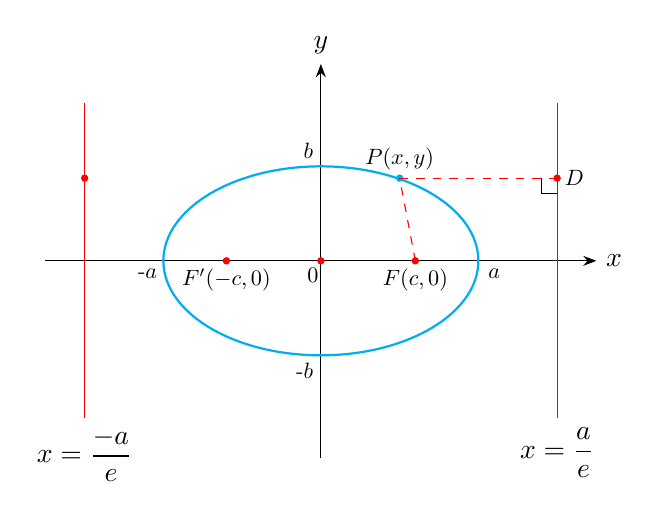
\begin{tikzpicture}[=>stealth]
\draw[-Stealth](-3.5,0)--(3.5,0)node[right]{$x$};
\draw[-Stealth](0,-2.5)--(0,2.5)node[above]{$y$};
\draw[thick,cyan](0,0)ellipse[x radius=2,y radius=1.2];
\draw(0,0)node[shape=circle, fill=red, scale=0.01cm]{}
(-1.2,0)node[shape=circle,fill=red,scale=0.01cm]{}
(1.2,0)node[shape=circle,fill=red,scale=0.01cm]{}
(-1.2,0)node[below,scale=0.8]{$F'(-c,0)$}
(1.2,0)node[below,scale=0.8]{$F(c,0)$}
(0,-1.4)node[left,scale=0.8]{-$b$}
(0,1.4)node[left,scale=0.8]{$b$}
(2.2,0)node[below,scale=0.8]{$a$}
(-2.2,0)node[below,scale=0.8]{-$a$}
(-0.1,0)node[below,scale=0.8]{$0$}
(1,1.05)node[shape=circle,fill=cyan,scale=0.01cm]{}
(3,1.05)node[shape=circle,fill=red,scale=0.01cm]{}
(-3,1.05)node[shape=circle,fill=red,scale=0.01cm]{}
(1,1.05)node[above,scale=0.8]{$P(x,y)$}
(3,1.05)node[right,scale=0.8]{$D$}
(-3,-2)node[below]{$x=\dfrac{-a}{e}$}
(3,-2)node[below]{$x=\dfrac{a}{e}$};
\draw((2.8,1.05)--(2.8,0.85)--(3,0.85);
\draw[red](-3,-2)--(-3,2);
\draw[red](3,-2)--(3,2);
\draw[dashed,red](1.2,0)--(1,1.05);
\draw[dashed,red](1,1.05)--(3,1.05);
\end{tikzpicture}
\end{figure}

It can be shown that the eccentricity of an ellipse with foci $(\pm c, 0)$ and vertices $(\pm a, 0)$ is $\dfrac{c}{a}$. i. e $\hspace{0.3cm} e = \dfrac{c}{a}$ the corresponding directions are $x = \pm \dfrac{a}{e}$.

\item If $e>1$, the conic is a hyperbola.

% DIAGRAM 11

\begin{figure}[H]
\centering
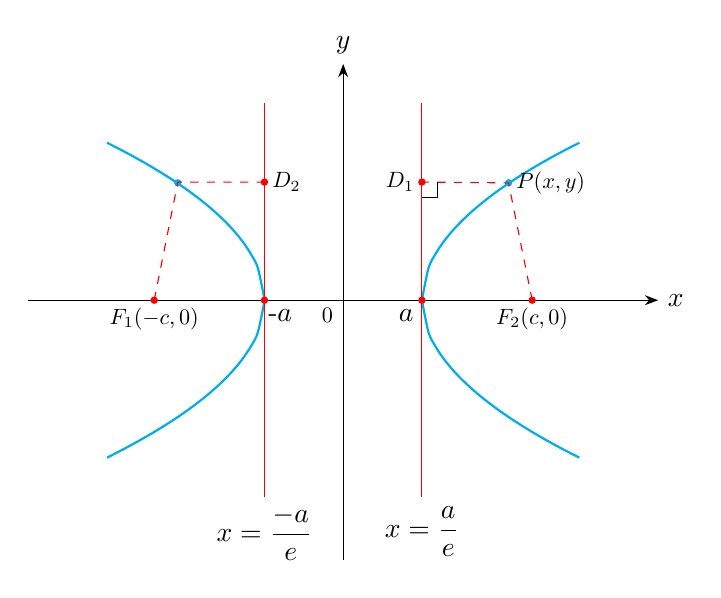
\begin{tikzpicture}[=>stealth]
\draw[-Stealth](-4,0)--(4,0)node[right]{$x$};
\draw[-Stealth](0,-3.3)--(0,3)node[above]{$y$};
\draw[smooth,thick,cyan,domain=1:3,variable=\x]plot(\x,{sqrt(2*(\x-1)});
\draw[smooth,thick,cyan,domain=1:3,variable=\x]plot(\x,{-sqrt(2*(\x-1)});
\draw[smooth,thick,cyan,domain=-3:-1,variable=\x]plot(\x,{sqrt(-2*(\x+1)});
\draw[smooth,thick,cyan,domain=-3:-1,variable=\x]plot(\x,{-sqrt(-2*(\x+1)});
\draw(2.4,0)node[shape=circle,fill=red, scale=0.01cm]{}
(-2.4,0)node[shape=circle,fill=red,scale=0.01cm]{}
(1,0)node[shape=circle,fill=red,scale=0.01cm]{}
(-1,0)node[shape=circle,fill=red,scale=0.01cm]{}
(2.4,0)node[below,scale=0.8]{$F_2(c,0)$}
(-2.4,0)node[below,scale=0.8]{$F_1(-c,0)$}
(2.1,1.49)node[shape=circle,fill=cyan,thick,scale=0.01cm]{}
(-2.1,1.49)node[shape=circle,fill=cyan,scale=0.01cm]{}
(2.1,1.49)node[right,scale=0.8]{$P(x,y)$}
(1,1.5)node[shape=circle,fill=red,scale=0.01cm]{}
(-1,1.5)node[shape=circle,fill=red,scale=0.01cm]{}
(1,1.5)node[left,scale=0.8]{$D_1$}
(-1,1.5)node[right,scale=0.8]{$D_2$}
(-1,-2.5)node[below]{$x=\dfrac{-a}{e}$}
(1,-2.5)node[below]{$x=\dfrac{a}{e}$}
(0.8,0)node[below]{$a$}
(-0.8,0)node[below]{-$a$}
(-0.2,0)node[below,scale=0.8]{$0$};
\draw[dashed,red](2.4,0)--(2.1,1.49)--(1,1.5);
\draw[dashed,red](-2.4,0)--(-2.1,1.5)--(-1,1.5);
\draw[red](1,-2.5)--(1,2.5);
\draw[red](-1,-2.5)--(-1,2.5);
\draw(1,1.3)--(1.2,1.3)--(1.2,1.5);
\end{tikzpicture}
\end{figure}

\begin{note}
 Directrices of an ellipse or hyperbola whose foci are $(0,\pm c)$ and vertices $(0,\pm a)$ are given by \hspace{0.2cm}$\boxed{y = \pm \dfrac{a}{e}}$
\end{note}
\end{enumerate}

\begin{exa}


A conic has foci $(\pm 3,0)$ and eccentricity $e = \dfrac{3}{5}$. Find 
\begin{enumerate}
\item its equation
\item the equations of its directrices.
\end{enumerate}
\end{exa}

\begin{solution}
\begin{enumerate}
\item From the foci, $c = 3$. Since $e = \dfrac{3}{5}< 1$, the conic is an ellipse.

$$\text{But}\hspace{0.3cm} e = \frac{c}{a} \hspace{0.2cm} \implies \hspace{0.2cm} a = \frac{3}{3/5} = 5$$
Thus, $b^2 = a^2 - c^2 = 25 - 9 = 16$

Therefore, the equation of the ellipse is \hspace{0.2cm}$\dfrac{x^2}{25} + \dfrac{y^2}{16} = 1$

\item The equations of the directrices are \hspace{0.2cm}$\displaystyle{x = \pm \dfrac{a}{e}\hspace{0.4cm}\text{i.e}\hspace{0.3cm} x = \pm \frac{5}{3/5} = \pm \frac{25}{3}}$

% DIAGRAM 12

\begin{figure}[H]
\centering
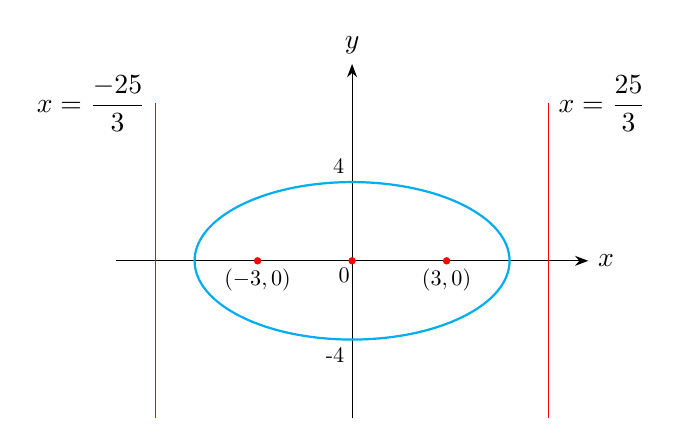
\begin{tikzpicture}[=>stealth]
\draw[-Stealth](-3,0)--(3,0)node[right]{$x$};
\draw[-Stealth](0,-2)--(0,2.5)node[above]{$y$};
\draw[thick,cyan](0,0)ellipse[x radius=2,y radius=1];
\draw(0,0)node[shape=circle, fill=red, scale=0.01cm]{}
(-1.2,0)node[shape=circle,fill=red,scale=0.01cm]{}
(1.2,0)node[shape=circle,fill=red,scale=0.01cm]{}
(-1.2,0)node[below,scale=0.8]{$(-3,0)$}
(1.2,0)node[below,scale=0.8]{$(3,0)$}
(0,-1.2)node[left,scale=0.8]{-$4$}
(0,1.2)node[left,scale=0.8]{$4$}
(-0.1,0)node[below,scale=0.8]{$0$}
(2.5,2)node[right]{$x=\dfrac{25}{3}$}
(-2.5,2)node[left]{$x=\dfrac{-25}{3}$};
\draw[red](2.5,-2)--(2.5,2)
(-2.5,-2)--(-2.5,2);
\end{tikzpicture}
\end{figure}

\end{enumerate}

\vspace{1cm}
\end{solution}
\subsection{Asymptotes of a Hyperbola}
When $x$ and $y$ both become very large the equation $$\frac{x^2}{a^2} - \frac{y^2}{b^2} = 1\hspace{0.5cm}\text{approximately} \hspace{0.5cm} \frac{x^2}{a^2}- \frac{y^2}{b^2} = 0$$

$$\Bigg(\dfrac{x}{a} - \dfrac{y}{b}\Bigg)\Bigg(\dfrac{x}{a} + \dfrac{y}{b}\Bigg) =0$$

Thus, the equations $\displaystyle{\dfrac{x}{a} - \dfrac{y}{b} = 0}$ and $\displaystyle{\dfrac{x}{a} + \dfrac{y}{b} = 0}$ are the asymptotes of a hyperbola.

% DIAGRAM 13

\begin{figure}[H]
\centering
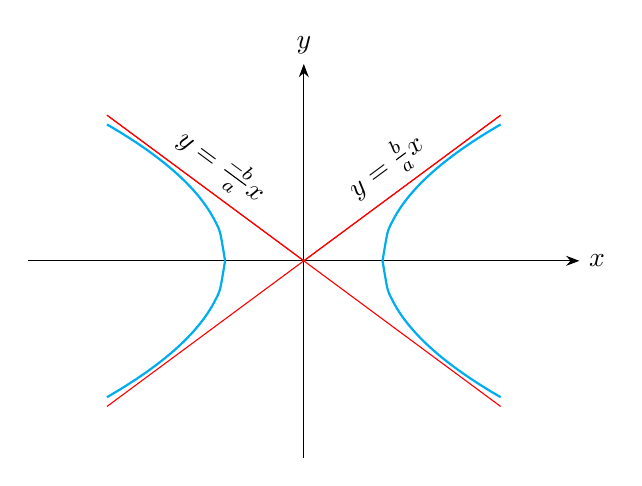
\begin{tikzpicture}[=>stealth]
\draw[-Stealth](-3.5,0)--(3.5,0)node[right]{$x$};
\draw[-Stealth](0,-2.5)--(0,2.5)node[above]{$y$};
\draw[smooth,thick,cyan,domain=1:2.5,variable=\x]plot(\x,{sqrt(2*(\x-1)});
\draw[smooth,thick,cyan,domain=1:2.5,variable=\x]plot(\x,{-sqrt(2*(\x-1)});
\draw[smooth,thick,cyan,domain=-2.5:-1,variable=\x]plot(\x,{sqrt(-2*(\x+1)});
\draw[smooth,thick,cyan,domain=-2.5:-1,variable=\x]plot(\x,{-sqrt(-2*(\x+1)});
\draw[red](-2.5,-1.85)--(2.5,1.85);
\draw[red](-2.5,1.85)--(2.5,-1.85);
\draw[red](0,0)--node[above,sloped,black]{$y=\frac{b}{a}x$}(2.5,1.85);
\draw[red](0,0)--node[above,sloped,black]{$y=\frac{-b}{a}x$}(-2.5,1.85);
\end{tikzpicture}
\end{figure}

\begin{exa}


The equations of the asympototes of a hyperbola $$\frac{x^2}{49} - \frac{y^2}{36} = 1$$ are $y = \dfrac{6}{7}x$ and $y = -\dfrac{6}{7}x$.


Similarly, the equations of the assymptotes of the hyperbola
$$\frac{y^2}{a^2} -\frac{x^2}{b^2} = 1$$ are given by $y = \pm \dfrac{a}{b}x$.

% DIAGRAM 14

\begin{figure}[H]
\centering
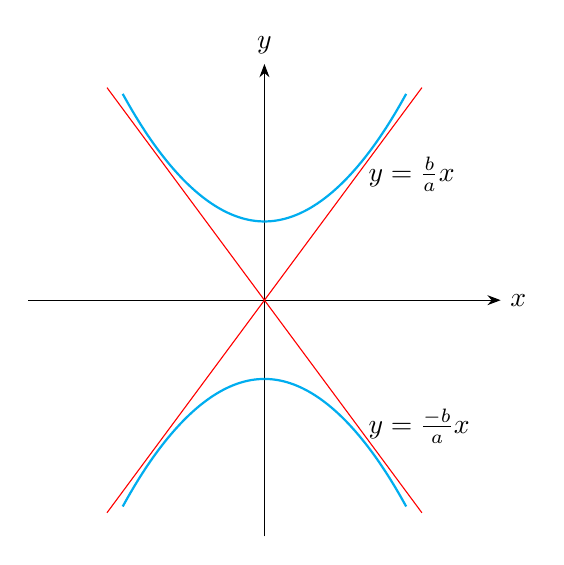
\begin{tikzpicture}[=>stealth]
\draw[-Stealth](-3,0)--(3,0)node[right]{$x$};
\draw[-Stealth](0,-3)--(0,3)node[above]{$y$};
\draw[red](-2,-2.7)--(2,2.7)
(2,-2.7)--(-2,2.7);
\draw[thick,cyan](0,1)parabola(1.8,2.62);
\draw[thick,cyan](0,1)parabola(-1.8,2.62);
\draw[thick,cyan](0,-1)parabola(1.8,-2.62);
\draw[thick,cyan](0,-1)parabola(-1.8,-2.62);
\draw(1.2,1.6)node[right]{$y=\frac{b}{a}x$}
(1.2,-1.6)node[right]{$y=\frac{-b}{a}x$};
\end{tikzpicture}
\end{figure}
\end{exa}

\begin{exa}


Discuss the graph of the conic
$$25y^2 - x^2 - 150y - 16x + 61 = 0$$
\end{exa}

\begin{solution}
\begin{align*}
25y^2 - 150y - x^2 - 16x + 61 & = 0\\
25\big(y^2 - 6y\big) - \big(x^2 + 16x\big) & = -61\\
25\big[(y-3)^2 - 9\big] - \big[(x+8)^2 - 64\big] & = -61\\
25(y-3)^2 - (x+8)^2 & = -61 + 225 - 64 = 100
\end{align*}

$$\dfrac{25(y - 3)^2}{100} - \dfrac{(x + 8)^2}{100} = \frac{100}{100}$$

$$\implies\hspace{0.5cm} \frac{(y - 3)^2}{4} - \frac{(x + 8)^2}{100} = 1$$

We let $X = x + 8$ and $Y = y -3$, then the equation becomes
$$\dfrac{Y^2}{4} - \dfrac{X^2}{100} = 1$$
Which is  a standard equation of a hyperbola whose foci lies on the $y-$axis.


In $X-Y$ coordinate system the origin is $(0,0)$, the vertices are $(0,\pm 2)$, the foci are $(0,\pm \sqrt{104})$.

$$e = \frac{c}{a} = \frac{\sqrt{104}}{2}$$

$$a = \frac{2\sqrt{13}}{5}\hspace{1cm} b = 2\sqrt{13}$$

$$c = \sqrt{\dfrac{52}{25} + 52} = \dfrac{2\sqrt{338}}{5}$$


Foci: $\hspace{0.2cm} \Bigg(0, \pm \dfrac{2\sqrt{338}}{5}\Bigg)\hspace{0.5cm}$ and $\hspace{0.5cm}$
Vertices: $\hspace{0.2cm} \Bigg( 0, \pm \dfrac{2\sqrt{13}}{5}\Bigg)$


$$e = \frac{c}{a} = \frac{2\sqrt{338}}{\dfrac{2\sqrt{13}}{5}\times 5} = \frac{\sqrt{338}}{\sqrt{13}} > 1 $$


The assymptotes are $Y =  \pm \dfrac{a}{b}X$ is $$Y = \pm \frac{\dfrac{2\sqrt{13}}{5}}{2\sqrt{13}}X\hspace{0.5cm} \implies\hspace{0.5cm} Y = \pm \frac{1}{5}X$$


The directrices are $Y = \pm \dfrac{a}{c}$ is $$Y = \pm \frac{\dfrac{2\sqrt{13}}{5}}{\dfrac{\sqrt{338}}{\sqrt{13}}}\hspace{0.5cm} \text{i.e}\hspace{0.5cm} Y = \pm \dfrac{26}{5\sqrt{338}}$$
\end{solution}


\begin{exa}


Analyze the equation $\hspace{0.4cm} x^2 - 4y^2 + 2x + 8y - 7 = 0$
\end{exa}


\begin{solution}
\begin{align*}
x^2 + 2x - 4(y^2 - 2y) & = 7\\
(x + 1)^2 - 4(y-1)^2 & = 7 + 1 - 4\\
\frac{(x+ 1)^2}{4} - \frac{4(y - 1)^2}{4} & = \frac{4}{4}\\\\
\frac{(x + 1)^2}{4} - \frac{(y - 1)^2}{1} & = 1\\
\end{align*}
Let $X = x + 1$ and $Y = y - 1$. Then the equation becomes
$$\frac{X^2}{4} - Y^2 = 1 ,$$
the standard equation of a hyperbola whose foci and vertices lie on the
$x-$axis.


In the new coordinate system
\begin{enumerate}
\item[] $\hspace{0.5cm}$ Origin (0,0)

\item[] $\hspace{0.5cm}$ Vertices:  $ a=2\hspace{0.3cm}$, $(-2,0)$ and $(2,0)$

\item[] $\hspace{0.5cm}$ Foci: $\hspace{0.2cm} c = \sqrt{b^2 + a^2} = \sqrt{4 + 1} = \sqrt{5}$. Hence $\hspace{0.2cm} (-\sqrt{5}, 0)$ and $(\sqrt{5},0)$.

\item[] $\hspace{0.5cm}$ Directrices: $\hspace{0.2cm} e  =\dfrac{c}{a} =\dfrac{\sqrt{5}}{2}> 1$. Thus $\hspace{0.2cm} X = \pm \dfrac{4}{\sqrt{5}}$.

\item[] $\hspace{0.5cm}$ ASymptotes: $\hspace{0.2cm} Y = \pm \dfrac{b}{a}X\hspace{0.3cm} \implies\hspace{0.3cm} Y = \pm \dfrac{1}{2}X$
\end{enumerate}

In the original coordinate system 
\begin{enumerate}
\item[] Centre: $\hspace{0.3cm} (-1,1)$

\item[] Vertices: $\hspace{0.3cm} (-3,1)$ and $(1,1)$

\item[] Foci: $\hspace{0.3cm} (\sqrt{5} -1, 1)$ and $(-\sqrt{5}-1, 1)$

\item[] Directrices: $\hspace{0.3cm} x + 1 = \pm \dfrac{4}{\sqrt{5}}$

\item[] Asymptotes: $\hspace{0.3cm} y - 1 = \pm \dfrac{1}{2} (x + 1)$
\end{enumerate}

% DIAGRAM 15

\begin{figure}[H]
\centering
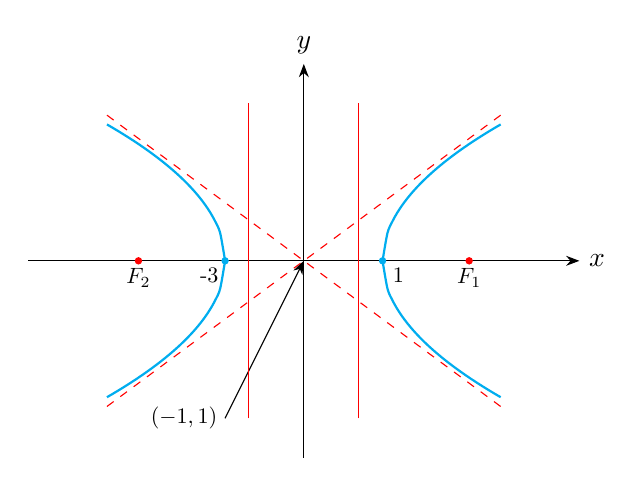
\begin{tikzpicture}[=>stealth]
\draw[-Stealth](-3.5,0)--(3.5,0)node[right]{$x$};
\draw[-Stealth](0,-2.5)--(0,2.5)node[above]{$y$};
\draw[smooth,thick,cyan,domain=1:2.5,variable=\x]plot(\x,{sqrt(2*(\x-1)});
\draw[smooth,thick,cyan,domain=1:2.5,variable=\x]plot(\x,{-sqrt(2*(\x-1)});
\draw[smooth,thick,cyan,domain=-2.5:-1,variable=\x]plot(\x,{sqrt(-2*(\x+1)});
\draw[smooth,thick,cyan,domain=-2.5:-1,variable=\x]plot(\x,{-sqrt(-2*(\x+1)});
\draw[red,dashed](-2.5,-1.85)--(2.5,1.85);
\draw[red,dashed](-2.5,1.85)--(2.5,-1.85);
\draw(2.1,0)node[shape=circle,fill=red,scale=0.01cm]{}
(-2.1,0)node[shape=circle,fill=red,scale=0.01cm]{}
(2.1,0)node[below,scale=0.8]{$F_1$}
(-2.1,0)node[below,scale=0.8]{$F_2$}
(-1,-2)node[left,scale=0.8]{$(-1,1)$}
(-1,0)node[shape=circle,scale=0.01cm,fill=cyan]{}
(1,0)node[shape=circle,scale=0.01cm,fill=cyan]{}
(1.2,0)node[below,scale=0.8]{1}
(-1.2,0)node[below,scale=0.8]{-3};
\draw[-Stealth](-1,-2)--(0,0);
\draw[red](0.7,-2)--(0.7,2);
\draw[red](-0.7,-2)--(-0.7,2);
\end{tikzpicture}
\end{figure}
\end{solution}

\subsection{Rotation of Axes}
A general equation of a conic section is given by $$Ax^2 + Bxy + Cy^2 + Dx + Ey + F = 0$$
Suppose that two rectangular coordinate system have the same origin and that $x'-y'$ coordinate system can be obtained by rotating the $x-y$ axes about the origin in the counter clockwise direction through angle $\alpha$.

% DIAGRAM 16

\begin{figure}[H]
\centering
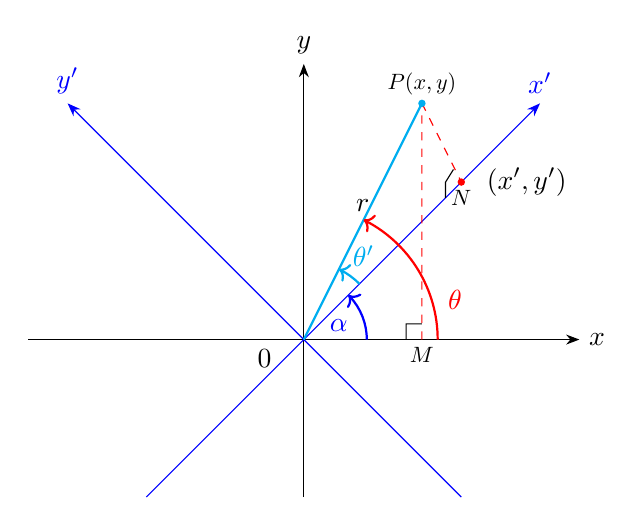
\begin{tikzpicture}[=>stealth]
\draw[-Stealth](-3.5,0)--(3.5,0)node[right]{$x$};
\draw[-Stealth](0,-2)--(0,3.5)node[above]{$y$};
\draw[blue,-Stealth](-2,-2)--(3,3)node[above]{$x'$};
\draw[blue,-Stealth](2,-2)--(-3,3)node[above]{$y'$};
\draw[thick,cyan](0,0)--(1.5,3);
\draw[dashed,red](1.5,0)--(1.5,3)
(1.5,3)--(2,2);
\draw(1.5,3)node[shape=circle,fill=cyan,scale=0.01cm]{}
(1.5,3)node[above,scale=0.8]{$P(x,y)$}
(1.5,0)node[below,scale=0.8]{$M$}
(0.75,1.5)node[above]{$r$}
(2,2)node[below,scale=0.8]{$N$}
(2,2)node[shape=circle,fill=red,scale=0.01cm]{}
(1.7,0.5)node[right,thick,red]{$\theta$}
(2.2,2)node[right]{$(x',y')$}
(-0.5,0)node[below]{$0$};
\coordinate (a) at (0.5,0);
\coordinate (b) at (0,0);
\coordinate (c) at (0.5,0.5);
\coordinate (d) at (0.5,1);
\draw
pic[thick,blue, draw=blue, ->, angle radius =0.8cm, "$\alpha$"]{angle=a--b--c};
\draw
pic[thick,cyan,draw=cyan,->, angle radius =1cm, angle eccentricity=1.3, "$\theta'$"]{angle =c--b--d};
\draw
pic[thick,red,draw=red,->,angle radius = 1.7cm]{angle = a--b--d};
\draw(1.5,0.2)--(1.3,0.2)--(1.3,0)
(1.8,1.8)--(1.8,2)--(1.9,2.16);
\end{tikzpicture}
\end{figure}

If $\left|OP\right| = r$ and $\langle POM = \theta$, then $x = r\cos \theta$ and $y = r\sin \theta$.\\

If $<PON = \theta'$, then $x' = r\cos \theta'$ and $y'= r\sin \theta'$.


But $\theta = \theta' + \alpha$. Thus $x = r\cos (\theta' + \alpha )$ and $y = r\sin (\theta' + \alpha)$.

\begin{align*}
x & = r\cos\theta'\cos \alpha -r\sin \theta'\sin \alpha\\
y & = r\sin\theta'\cos\alpha + r \cos\theta'\sin\alpha\\
\end{align*}

\begin{align*}
x & = x'\cos\alpha - y'\sin \alpha\\
\implies \hspace{0.4cm} & \hspace{4cm} \cdots\cdots\cdots\hspace{0.2cm} (I)\\
y & = y'\cos \alpha + x'\sin \alpha
\end{align*}

Solving $(I)$ simultaneously for $x'$ and $y'$ yields
$$(II)\hspace{0.5cm}\cdots\cdots\cdots\hspace{0.8cm} 
\begin{cases}
x' & = x\cos \alpha + y\sin \alpha\\
y' & = -x\sin \alpha + y\cos \alpha
\end{cases}
$$

These are the rotation equations which relate the $x-y$ system and $x'-y'$ system.


Rotating the axes through an angle of $\alpha$, leaves the curve unchanged by changes the equation into $$A'x'^2 + B'x'y' + C'y'^2 + D'y'^2 + E'y' + F' = 0$$ 
The coefficients $A', B', C', D', E'$ and $F'$ are related with $A, B, C, D, E$ and $F$ are as follows:

\begin{align*}
A' & = A\cos^2\alpha + B\cos\alpha\sin\alpha + C\sin^2\alpha\\
B' &  = B(\cos^2\alpha - \sin^2\alpha) + 2(C-A)\sin\alpha\cos\alpha\\
C' & = A\sin^2 \alpha - B\sin \alpha \cos \alpha + C\cos^2\alpha\\
D' & = D\cos \alpha + E\sin \alpha\\
E' &  = -D\sin \alpha + E \cos \alpha\\
F' & = F\\
\end{align*}

To remove the $xy$ term we merely set $B' =0$. This means that $$B(\cos^2\alpha - \sin^2\alpha) = 2(A-C)\sin\alpha\cos\alpha$$

$$\implies\hspace{0.4cm} \frac{\cos 2\alpha}{\sin 2\alpha} = \frac{A - C}{B}\hspace{0.3cm} \text{if}\hspace{0.3cm} B\neq 0$$

$$\text{or}\hspace{0.3cm} \cot 2\alpha = \dfrac{A - C}{B}\hspace{0.3cm} \text{if}\hspace{0.3cm} B \neq 0$$

Equation $(II)$ is used to remove the $xy$ term in the general equation.
$$Ax^2 + Bxy + Cy^2 + Dx + Ey + F = 0$$

Any $B\neq 0$ leads to a unique value of $2\alpha$ in the interval $0< 2\alpha <\pi$ and hence determine a unique $\alpha$ in the interval $0< \alpha < \dfrac{\pi}{2}$.


\begin{exa}


Discuss the graph of $\hspace{0.2cm}6xy + 8y^2 - 12x - 26y + 11 = 0$
\end{exa}


\begin{solution}
$$A = 0\hspace{0.2cm},\hspace{0.2cm} B = 6 \hspace{0.2cm},\hspace{0.2cm} C = 8 \hspace{0.2cm},\hspace{0.2cm} D = -12 \hspace{0.2cm},\hspace{0.2cm} E = -26 \hspace{0.2cm},\hspace{0.2cm} F = 11$$

$$\cot 2\alpha = \frac{A - B}{C} = \frac{0-8}{6} = \frac{-4}{3}$$

% DIAGRAM 17

\begin{figure}[H]
\centering
\begin{tikzpicture}[=>stealth]
\draw[-Stealth](-3,0)--(2,0);
\draw[-Stealth](0,-1)--(0,2.5);
\draw[thick,cyan,-Stealth](0,0)--(-2,1.5);
\draw[red,dashed](-2,0)--(-2,1.5)--(0,1.5);
\draw(0,1.5)node[right]{3}
(-2,0.75)node[left]{3}
(-1,0.75)node[above]{5}
(-2,0)node[below]{-4};
\coordinate (a) at (0.5,0);
\coordinate (b) at (0,0);
\coordinate (c) at (-0.75,0.56);
\draw
pic[thick, draw=red,->,angle radius=0.5cm, "$2\alpha$", angle eccentricity = 1.5]{angle = a--b--c};
\end{tikzpicture}
\end{figure}

 $$\text{But}\hspace{0.3cm} \cos \alpha = \sqrt{\dfrac{1}{2}(1 + \cos 2\alpha)} = \sqrt{\dfrac{1}{2}\Big( 1 - \dfrac{4}{5}\Big)} = \frac{1}{\sqrt{10}}$$

$$\sin \alpha = \sqrt{\dfrac{1}{2}(1 - \cos 2\alpha)}=\sqrt{\dfrac{1}{2}\Big(1 + \dfrac{4}{5}\Big)} = \dfrac{3}{\sqrt{10}}$$

\begin{align*}
x & = x'\cos \alpha - y'\sin \alpha = \dfrac{x'}{\sqrt{10}} - \dfrac{3y'}{\sqrt{10}}= \dfrac{x' - 3y'}{\sqrt{10}}\\\\
y & = x'\sin \alpha + y'\cos \alpha = \dfrac{3x' + y'}{\sqrt{10}}\\
\end{align*}

Substituting these in the equation we have
$$6xy + 8y^2 - 12x - 26y + 11 = 0$$

$$6\Bigg(\dfrac{x' - 3y'}{\sqrt{10}}\Bigg)\Bigg(\dfrac{3x' + y'}{\sqrt{10}}\Bigg) + 8\Bigg(\dfrac{3x' + y'}{\sqrt{10}}\Bigg)^2 - 12\Bigg(\frac{x' - 3y'}{\sqrt{10}}\Bigg) - 26\Bigg(\frac{3x' + y'}{\sqrt{10}}\Bigg) + 11 = 0$$

$$\implies\hspace{0.5cm} \dfrac{6}{10}\Big(3x'^2 - 8x'y' - 3y'^2\Big) + \dfrac{8}{10}\Big(9x'^2 + 6x'y' + y'^2\Big) - \dfrac{12}{\sqrt{10}}\Big(x' - 3y'\Big) - \dfrac{26}{\sqrt{10}}\Big(3x' + y'\Big) + 11 = 0$$

$$\implies\hspace{0.5cm} 18x'^2 - 48x'y' - 18y'^2 + 72x'^2 + 48x'y' + 8y'^2 - 12\sqrt{10}x' + 36\sqrt{10}y' - 78\sqrt{10}x' - 26\sqrt{10}y' + 110 = 0$$

$$\implies\hspace{0.5cm} 90x'^2 - 90\sqrt{10}x' - 10y'^2 + 10\sqrt{10}y' + 110 = 0$$

To identify this conic we need to translate the axes by completing the square of the rearranged term as follows:

\begin{align*}
90\Big( x'^2 -\sqrt{10}x' + \frac{10}{4} - \frac{10}{4}\Big) - 10\Big(y'^2 - \sqrt{10}y' +\frac{10}{4} - \frac{10}{4}\Big) + 110 & = 0\\\\
9\Big(x'^2 - \sqrt{10}x' + \frac{5}{2} - \frac{5}{2}\Big) - \Big(y'^2 - \sqrt{10}y' + \frac{5}{2} - \frac{5}{2}\Big) + 11 & = 0\\\\
9\Big(x' - \dfrac{\sqrt{10}}{2}\Big)^2 - \dfrac{45}{2} - \Big(y' - \dfrac{\sqrt{10}}{2}\Big)^2 + \frac{5}{2} + 11 & = 0\\\\
9\Bigg(x' -\dfrac{\sqrt{10}}{2}\Bigg)^2 - \Bigg(y' - \dfrac{\sqrt{10}}{2}\Bigg)^2 & = 9\\
\end{align*}

$$\implies\hspace{0.5cm} \frac{\Big(x' - \dfrac{\sqrt{10}}{2}\Big)^2}{1} - \frac{\Big(y' - \dfrac{\sqrt{10}}{2}\Big)^2}{9}=1$$


Let $\hspace{0.2cm} X = x' - \dfrac{10}{2}\hspace{0.2cm}$ and $\hspace{0.2cm} Y = y' - \dfrac{\sqrt{10}}{2}\hspace{0.2cm}$. Then the equations becomes $$\dfrac{X^2}{1}- \dfrac{Y^2}{9} = 1$$ Which is a standard equation of a hyperbola. Hence $$a = 1\hspace{0.2cm},\hspace{0.2cm}b = 3\hspace{0.2cm},\hspace{0.2cm} c = \sqrt{10}\hspace{0.2cm}\implies\hspace{0.2cm} e = \sqrt{10}$$

In the $X-Y$ system
\begin{enumerate}
\item[] Centre: $\hspace{0.3cm} (0,0)$

\item[] Vertices: $\hspace{0.3cm}(\pm 1, 0)$

\item[] Foci: $\hspace{0.3cm} (\pm \sqrt{10}, 0)$

\item[] Directrices: $\hspace{0.3cm} X = \pm \dfrac{1}{\sqrt{10}}$

\item[] Asymptotes: $\hspace{0.3cm} Y = \pm 3X$
\end{enumerate}

In the $x'-y'$ system the
\begin{enumerate}
\item[] Centre: $\hspace{0.3cm} \Bigg(\dfrac{\sqrt{10}}{2},\dfrac{\sqrt{10}}{2}\Bigg)$

\item[] Vertices: $\hspace{0.3cm} \Bigg( \dfrac{2 + \sqrt{10}}{2},\dfrac{\sqrt{10}}{2}\Bigg) \hspace{0.2cm},\hspace{0.2cm} \Bigg( \dfrac{-2 + \sqrt{10}}{2},\dfrac{\sqrt{10}}{2}\Bigg)$

\item[] Foci: $\hspace{0.3cm}\Bigg(\dfrac{3\sqrt{10}}{2},\dfrac{\sqrt{10}}{2}\Bigg)\hspace{0.2cm},\hspace{0.2cm} \Bigg(\dfrac{-3\sqrt{10}}{2},\dfrac{\sqrt{10}}{2}\Bigg)$

\item[] Directrices: $\hspace{0.3cm} x' - \dfrac{\sqrt{10}}{2} = \pm \dfrac{1}{\sqrt{10}}$

\item[] Asymptotes: $\hspace{0.3cm} y' - \dfrac{\sqrt{10}}{2} = \pm 3\Bigg( x' - \dfrac{\sqrt{10}}{2}\Bigg)$
\end{enumerate}

\begin{align*}
x = \dfrac{x' - 3y'}{\sqrt{10}}\hspace{0.3cm} &,\hspace{0.3cm} y = \dfrac{3x' + y'}{\sqrt{10}}\\\\
y' = \dfrac{-3x + y}{\sqrt{10}} \hspace{0.3cm} &,\hspace{0.3cm} x' = \frac{x + 3y}{\sqrt{10}}\\
\end{align*}

In the $x-y$ system
\begin{enumerate}
\item[] Centre: $\hspace{0.3cm} (-1,3)$

\item[] Vertices: $\hspace{0.3cm} (1+\sqrt{10}, 3+2\sqrt{10})\hspace{0.3cm},\hspace{0.3cm} (\sqrt{10} + 1, 3 + 2\sqrt{10})$

\item[] Foci: $\hspace{0.3cm} (0,5)\hspace{0.2cm},\hspace{0.2cm} (-2,-1)$

\item[] Directrices: $\hspace{0.3cm} \dfrac{x + 3y}{\sqrt{10}} - \dfrac{\sqrt{10}}{2} = \pm \dfrac{1}{\sqrt{10}}$

\item[] Asymptotes: $\hspace{0.3cm} \dfrac{-3x + y}{\sqrt{10}} - \dfrac{\sqrt{10}}{2}  = \pm 3\Bigg(\dfrac{x + 3y}{\sqrt{10}} - \dfrac{\sqrt{10}}{2}\Bigg)$
\end{enumerate}

From the general equation of the conic section $$Ax^2 + Bxy + Cy^2 + Dx + Ey + F = 0$$

The graph represents
\begin{enumerate}
\item a hyperbola if $B^2 - 4AC > 0$
\item a parabola if $B^2 - 4AC = 0$
\item an ellipse if $B^2 - 4AC <0$
\end{enumerate}

\vspace{1cm}
\end{solution}

\subsection{Conics in Polar Coordinates}

A conic section is a collection of $P$ such that $$\dfrac{\left|PF\right|
}{\left|PD\right|
} = e \hspace{0.3cm}\cdots\cdots\cdots\hspace{0.3cm} (I)  $$

where $\left|PF\right|$ is the distance from $P$ to the focus and $\left|PD\right|$ is the distance from $P$ to the directrix and $e$ is the eccentricity.

% DIAGRAM 18

\begin{figure}[H]
\centering
\begin{tikzpicture}[=>stealth]
\draw[-Stealth](-2.5,0)--(3.5,0)node[right]{$x$};
\draw[-Stealth](0.5,-3)--(0.5,3)node[above]{$y$};
\draw[smooth,thick,cyan,domain=0:2,variable=\x]plot(\x,{sqrt(2*\x)});
\draw[smooth,thick,cyan,domain=0:2,variable=\x]plot(\x,{-sqrt(2*\x)});
\draw[violet,thick](0.5,0)--(1.5,1.75);
\draw[red](-1,-2.5)--(-1,2.5);
\draw[red,dashed](1.5,1.75)--(-1,1.75);
\draw(1.5,1.75)node[shape=circle,fill=cyan,scale=0.01cm]{}
(-1,1.75)node[shape=circle,fill=red,scale=0.01cm]{}
(0.5,0)node[shape=circle,fill=red,scale=0.01cm]{}
(0,0)node[shape=circle,fill=cyan,scale=0.01cm]{}
(-1,-2.5)node[below]{$x =- p$}
(-1,1.75)node[left,scale=0.8]{$D$}
(1.5,1.6)node[right,scale=0.8]{$P(r,\theta)$}
(0.7,0)node[below,scale=0.8]{$F$}
(0.4,0)node[below,scale=0.8]{$0$}
(1,0.9)node[above]{$r$};
\draw(-1,1.55)--(-0.8,1.55)--(-0.8,1.75);
\coordinate (a) at (1,0);
\coordinate (b) at (0.5,0);
\coordinate (c) at (1,0.9);
\draw
pic[draw=violet,thick,angle radius=0.5cm,->, angle eccentricity =1.4,"$\theta$"]{angle=a--b--c};
\end{tikzpicture}
\end{figure}

$$\left|PD\right|  = P + r\cos \theta $$

Further, $\left|PF\right|=r$, and so if $P$ is on the cone, described by $(I)$ then $$\dfrac{r}{P + r\cos \theta} =e\hspace{0.3cm}\cdots\cdots\cdots\hspace{0.3cm} (1)$$

Solving for $r$, we have
$$r = \frac{eP}{1 - e\cos \theta}\hspace{0.4cm}\cdots\cdots\cdots\hspace{0.4cm} (II)$$

which is a polar equation of a conic section whose focus is at the origin and directrix is $P$ units to the left of the focus.


\begin{exa}


Describe the graph of \hspace{0.2cm}$r = \dfrac{8}{1 - 2\cos \theta}$
\end{exa}


\begin{solution}


We write the given equation in the form of equation $(II)$


i.e $\hspace{0.3cm} r = \dfrac{8}{1 - 2\cos \theta} = \dfrac{2(4)}{1 - 2\cos \theta}$


$\implies\hspace{0.3cm} e = 2$ and $P = 4$, since $e>1$ the curve is a hyperbola whose focus is at the origin and its associated directrix is 4 units to the left of the focus.
\end{solution}


\begin{note}
\begin{enumerate}
\item The polar equation of a conic which has one focus at the origin and directrix $P$ units to the right of the origin is given by $$r = \dfrac{eP}{1 + e\cos \theta} \hspace{0.3cm}\cdots\cdots\cdots\hspace{0.4cm} (III)$$

\item The polar equation of a conic which has one focus at the origin and directrix $P$ units below the origin is given by $$r = \frac{eP}{ 1 -e\sin \theta}\hspace{0.3cm} \cdots\cdots\cdots\hspace{0.4cm} (IV)$$

\item Similarly $$r = \frac{eP}{1 + e\sin \theta}\hspace{0.4cm}\cdots\cdots\cdots\hspace{0.3cm} (V)$$
represents the polar equation of a conic which has the focus at the origin and directrix $P$ units above the origin.
\end{enumerate}
\end{note}

\begin{exa}


Identify the conic section and give its eccentricity and the distance of the directrix from the origin. Hence sketch the curve.
$$(1)\hspace{0.6cm} r = \dfrac{5}{2 + \cos \theta}\hspace{2cm} (2)\hspace{0.6cm} r = \frac{7}{2 - 5\sin \theta}$$
\end{exa}


\begin{solution}
\begin{enumerate}
\item \begin{align*}
r & = \frac{eP}{1 + e\cos \theta}\\
& = \frac{5}{2 + \cos \theta} = \frac{5}{2\Big[1 + \dfrac{1}{2}\cos \theta \Big]}\\
& = \frac{5/2}{1 + \dfrac{1}{2}\cos \theta}\\
& = \frac{\Big(\dfrac{1}{2}\Big)\hspace{0.1cm}(5)}{1 + \dfrac{1}{2}\cos \theta}
\end{align*}

$\implies\hspace{0.5cm} e = \dfrac{1}{2}< 1 \hspace{0.3cm} \implies \hspace{0.3cm}$ the eccentricity is $\dfrac{1}{2}$ and the conic is an ellipse.

$P = 5\hspace{0.3cm}$ the  directrix is 5 units on the right hand sided of the origin $x = 5$.

$$(r,\theta)$$

% DIAGRAM 19

\begin{figure}[H]
\centering
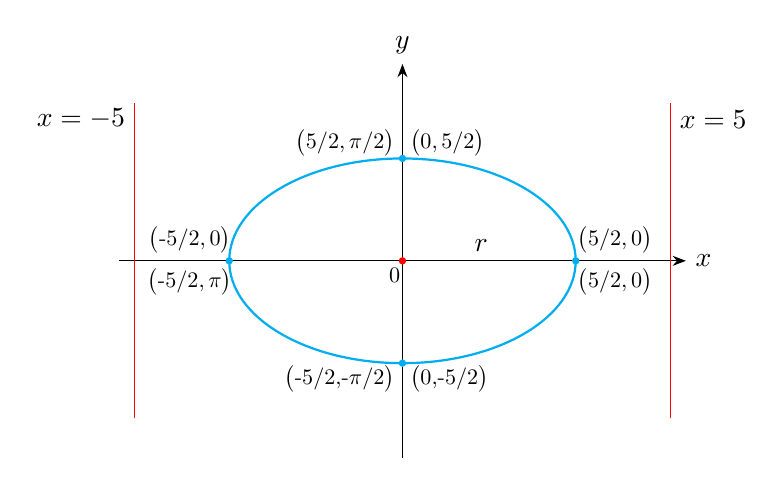
\begin{tikzpicture}[=>stealth]
\draw[-Stealth](-3.6,0)--(3.6,0)node[right]{$x$};
\draw[-Stealth](0,-2.5)--(0,2.5)node[above]{$y$};
\draw[thick,cyan](0,0)ellipse[x radius=2.2,y radius=1.3];
\draw(0,0)node[shape=circle, fill=red, scale=0.01cm]{}
(2.2,0)node[shape=circle,fill=cyan,scale=0.01cm]{}
(-2.2,0)node[shape=circle,fill=cyan,scale=0.01cm]{}
(0,1.3)node[shape=circle,fill=cyan,scale=0.01cm]{}
(0,-1.3)node[shape=circle,fill=cyan,scale=0.01cm]{}
(-0.1,0)node[below,scale=0.8]{$0$}
(0,1.5)node[right,scale=0.8]{$\big(0,5/2\big)$}
(0,1.5)node[left,scale=0.8]{$\big(5/2,\pi/2\big)$}
(2.7,0)node[above,scale=0.8]{$\big(5/2,0\big)$}
(2.7,0)node[below,scale=0.8]{$\big(5/2,0\big)$}
(-2.7,0)node[above,scale=0.8]{$\big($-$5/2,0\big)$}
(-2.7,0)node[below,scale=0.8]{$\big($-$5/2,\pi\big)$}
(0,-1.5)node[right,scale=0.8]{$\big(0,$-$5/2\big)$}
(0,-1.5)node[left,scale=0.8]{$\big($-$5/2,$-$\pi/2\big)$}
(1,0)node[above]{$r$}
(3.4,1.8)node[right]{$x=5$}
(-3.4,1.8)node[left]{$x=-5$};
\draw[red](3.4,-2)--(3.4,2)
(-3.4,-2)--(-3.4,2);
\end{tikzpicture}
\end{figure}

\item
\begin{align*}
r & = \frac{7}{2 - 5\sin \theta}= \frac{7}{2\Big[1 - \dfrac{5}{2}\sin \theta\Big]}\\
& = \frac{7/2}{1 - \dfrac{5}{2}\sin\theta}\\\\
& = \frac{(5/2)(7/5)}{1-\dfrac{5}{2}\sin \theta}
\end{align*}

$\therefore\hspace{0.3cm} e = \dfrac{5}{2}>1 \implies $ the conic is a hyperbola.

$P = \dfrac{7}{5} \implies$ the directrix is $\dfrac{7}{5}$ units below the $x-$axis.

% DIAGRAM 20
\begin{figure}[H]
\centering
\begin{tikzpicture}[=>stealth]
\draw[-Stealth](-3,0)--(3,0)node[right]{$x$};
\draw[-Stealth](0,-5)--(0,2)node[above]{$y$};
\draw[thick,cyan](0,-1)parabola(2,1);
\draw[thick,cyan](0,-1)parabola(-2,1);
\draw[thick,cyan](0,-3)parabola(2,-5);
\draw[thick,cyan](0,-3)parabola(-2,-5);
\draw[red](-3,-2)--(3,-2);
\draw(-1.42,0)node[shape=circle,fill=cyan,scale=0.01cm]{}
(0,-1)node[shape=circle,fill=cyan,scale=0.01cm]{}
(1.42,0)node[shape=circle,fill=cyan,scale=0.01cm]{}
(1.8,0)node[below,scale=0.8]{$(7/2,0)$}
(-1.9,0)node[below,scale=0.8]{$(7/2,-\pi)$}
(0,-1.2)node[right,scale=0.8]{$(1,-\pi/2)$}
(3,-2)node[right]{$y=\dfrac{-7}{5}$};
\end{tikzpicture}
\end{figure}
\end{enumerate} 

\pagebreak
\end{solution}

\subsection{Practice Problems}

These are the tutorial questions for this section, worked in full.

\begin{problem}
Sketch each parabola and give the coordinates of the focus and the equation of
the directrix.
$$(a)\hspace{0.3cm} 7y = -5x^2 \hspace{2.5cm} (b)\hspace{0.3cm} x = -\frac{y^2}{8}$$
\end{problem}
\begin{solution}
\subhead{(a)}
Write it in standard form: $x^2 = -\dfrac{7}{5}y$. Comparing with $x^2 = -4py$
gives $4p = \dfrac{7}{5}$, so $p = \dfrac{7}{20}$. The parabola opens downward
with vertex at the origin, focus $\Big(0, -\dfrac{7}{20}\Big)$ and directrix
$y = \dfrac{7}{20}$.

\subhead{(b)}
Here $y^2 = -8x$. Comparing with $y^2 = -4px$ gives $4p = 8$, so $p = 2$. The
parabola opens to the left with vertex at the origin, focus $(-2, 0)$ and
directrix $x = 2$.
\end{solution}

\begin{problem}
Derive the equation of the parabola with focus $(4,5)$ and directrix $y = -1$.
\end{problem}
\begin{solution}
A point $P(x,y)$ lies on the parabola when its distance to the focus equals its
distance to the directrix:
$$\sqrt{(x-4)^2 + (y-5)^2} = \left|y + 1\right| .$$
Squaring,
$$x^2 - 8x + 16 + y^2 - 10y + 25 = y^2 + 2y + 1
\hspace{0.4cm}\implies\hspace{0.4cm} x^2 - 8x + 40 = 12y .$$
Completing the square, $(x-4)^2 = 12(y-2)$. The vertex is $(4,2)$, midway
between the focus and the directrix as it must be, and $4p = 12$ so $p = 3$.
\end{solution}

\begin{problem}
Write the standard form of the equation of each ellipse.
\begin{enumerate}
\item[(a)] Distance sum $10$, foci $(\pm 3, 0)$.
\item[(b)] Distance sum $20$, foci $(0, \pm 6)$.
\end{enumerate}
\end{problem}
\begin{solution}
The distance sum is $2a$ and the foci are at distance $c$ from the centre, with
$b^2 = a^2 - c^2$.

\subhead{(a)}
$2a = 10$ so $a = 5$, and $c = 3$, giving $b^2 = 25 - 9 = 16$. The foci are on
the $x-$axis, so
$$\frac{x^2}{25} + \frac{y^2}{16} = 1 .$$

\subhead{(b)}
$2a = 20$ so $a = 10$, and $c = 6$, giving $b^2 = 100 - 36 = 64$. The foci are on
the $y-$axis, so the larger denominator belongs to $y$:
$$\frac{x^2}{64} + \frac{y^2}{100} = 1 .$$
\end{solution}

\begin{problem}
Find the foci and distance sum for each ellipse.
$$(a)\hspace{0.3cm}\frac{x^2}{25} + \frac{y^2}{9} = 1
\hspace{2.5cm} (b)\hspace{0.3cm}\frac{x^2}{9} + \frac{y^2}{25} = 1$$
\end{problem}
\begin{solution}
\subhead{(a)}
The larger denominator is under $x$, so $a^2 = 25$, $b^2 = 9$ and the major axis
is horizontal. Then $c^2 = 25 - 9 = 16$, so $c = 4$: foci $(\pm 4, 0)$ and
distance sum $2a = 10$.

\subhead{(b)}
The same numbers with the roles of $x$ and $y$ exchanged: $a^2 = 25$ under $y$,
so the major axis is vertical, $c = 4$, foci $(0, \pm 4)$ and distance sum $10$.
\end{solution}

\begin{problem}
Find the ellipse in standard form passing through $(4,-1)$ and $(-2,-2)$.
\end{problem}
\begin{solution}
Take the ellipse centred at the origin with axes along the coordinate axes,
$$\frac{x^2}{A} + \frac{y^2}{B} = 1 .$$
Substituting the two points gives
$$\frac{16}{A} + \frac{1}{B} = 1, \qquad \frac{4}{A} + \frac{4}{B} = 1 .$$
Multiply the first by $4$ and subtract the second:
$$\frac{64}{A} - \frac{4}{A} = 3 \implies \frac{60}{A} = 3 \implies A = 20 .$$
Then $\dfrac{16}{20} + \dfrac{1}{B} = 1$ gives $\dfrac{1}{B} = \dfrac{1}{5}$, so
$B = 5$. Hence
$$\frac{x^2}{20} + \frac{y^2}{5} = 1 .$$
\end{solution}

\begin{problem}
Write the standard form of the equation of the hyperbola with
\begin{enumerate}
\item[(a)] $\pm\big(\left|PF_1\right| - \left|PF_2\right|\big) = 8$ and foci
$(\pm 5, 0)$;
\item[(b)] the same distance difference and foci $(0, \pm 5)$.
\end{enumerate}
\end{problem}
\begin{solution}
The distance difference is $2a$ and $b^2 = c^2 - a^2$.

\subhead{(a)}
$2a = 8$ so $a = 4$, and $c = 5$, giving $b^2 = 25 - 16 = 9$. The foci are on the
$x-$axis, so
$$\frac{x^2}{16} - \frac{y^2}{9} = 1 .$$

\subhead{(b)}
The same values with the foci on the $y-$axis, so the positive term is in $y$:
$$\frac{y^2}{16} - \frac{x^2}{9} = 1 .$$
\end{solution}

\begin{problem}
Find the foci and distance difference for each hyperbola.
$$(a)\hspace{0.3cm}\frac{x^2}{25} - \frac{y^2}{144} = 1
\hspace{2.5cm} (b)\hspace{0.3cm}\frac{y^2}{25} - \frac{x^2}{144} = 1$$
\end{problem}
\begin{solution}
For a hyperbola it is the sign, not the size of the denominators, that fixes the
axis, and $c^2 = a^2 + b^2$ in both cases with $a^2$ under the positive term.

\subhead{(a)}
$a^2 = 25$, $b^2 = 144$, so $c^2 = 169$ and $c = 13$: foci $(\pm 13, 0)$ and
distance difference $2a = 10$.

\subhead{(b)}
The positive term is in $y$, so the curve opens vertically: foci $(0, \pm 13)$
and distance difference $10$.
\end{solution}

\begin{problem}
Find the equation of the hyperbola through $(2,3)$ with foci $(\pm 2, 0)$.
\end{problem}
\begin{solution}
The foci are on the $x-$axis with $c = 2$, so $a^2 + b^2 = 4$ and
$b^2 = 4 - a^2$. Substituting the point $(2,3)$ into
$\dfrac{x^2}{a^2} - \dfrac{y^2}{b^2} = 1$,
$$\frac{4}{a^2} - \frac{9}{4-a^2} = 1 .$$
Multiplying by $a^2(4-a^2)$,
$$16 - 13a^2 = 4a^2 - a^4 \implies a^4 - 17a^2 + 16 = 0
\implies \big(a^2-1\big)\big(a^2-16\big) = 0 .$$
Since $a^2 < c^2 = 4$, we take $a^2 = 1$ and $b^2 = 3$:
$$x^2 - \frac{y^2}{3} = 1 ,$$
which checks: $4 - \dfrac{9}{3} = 1$.
\end{solution}

\begin{note}
In questions 9 to 17 the method is the same throughout: group the $x$ terms and
the $y$ terms, complete the square in each, and read off the type from the
signs. Two squared terms with the same sign give an ellipse, opposite signs a
hyperbola, and only one squared term a parabola.
\end{note}

\begin{problem}
Discuss the curve $\hspace{0.2cm} 9x^2 + 25y^2 - 90x - 150y + 225 = 0$.
\end{problem}
\begin{solution}
$$9\big(x^2-10x\big) + 25\big(y^2-6y\big) = -225$$
$$9(x-5)^2 - 225 + 25(y-3)^2 - 225 = -225
\implies 9(x-5)^2 + 25(y-3)^2 = 225 .$$
Dividing by $225$,
$$\frac{(x-5)^2}{25} + \frac{(y-3)^2}{9} = 1 .$$
An \emph{ellipse}, centre $(5,3)$, $a = 5$, $b = 3$, $c = 4$. Major axis
horizontal, vertices $(0,3)$ and $(10,3)$, foci $(1,3)$ and $(9,3)$,
$e = \dfrac{4}{5}$.
\end{solution}

\begin{problem}
Discuss the curve $\hspace{0.2cm} 16y^2 - 9x^2 - 64y - 54x = 161$.
\end{problem}
\begin{solution}
$$16(y-2)^2 - 64 - 9(x+3)^2 + 81 = 161
\implies 16(y-2)^2 - 9(x+3)^2 = 144 ,$$
$$\frac{(y-2)^2}{9} - \frac{(x+3)^2}{16} = 1 .$$
A \emph{hyperbola}, centre $(-3,2)$, opening vertically since the positive term
is in $y$. Here $a = 3$, $b = 4$, $c = 5$: vertices $(-3, 2\pm 3)$, foci
$(-3, 2\pm 5)$, asymptotes $y - 2 = \pm\dfrac{3}{4}(x+3)$, $e = \dfrac{5}{3}$.
\end{solution}

\begin{problem}
Discuss the curve $\hspace{0.2cm} x^2 + 2x + 16y + 33 = 0$.
\end{problem}
\begin{solution}
Only $x$ is squared, so this is a \emph{parabola}.
$$(x+1)^2 - 1 + 16y + 33 = 0 \implies (x+1)^2 = -16(y+2) .$$
Vertex $(-1,-2)$, opening downward, $4p = 16$ so $p = 4$: focus $(-1,-6)$ and
directrix $y = 2$.
\end{solution}

\begin{problem}
Discuss the curve $\hspace{0.2cm} 16x^2 + y^2 - 32x + 4y + 16 = 0$.
\end{problem}
\begin{solution}
$$16(x-1)^2 - 16 + (y+2)^2 - 4 + 16 = 0 \implies 16(x-1)^2 + (y+2)^2 = 4 ,$$
$$\frac{(x-1)^2}{\frac{1}{4}} + \frac{(y+2)^2}{4} = 1 .$$
An \emph{ellipse}, centre $(1,-2)$, with $a^2 = 4$ under $y$ so the major axis
is vertical: $a = 2$, $b = \dfrac{1}{2}$, and
$c = \sqrt{4 - \frac14} = \dfrac{\sqrt{15}}{2}$. Foci
$\Big(1, -2 \pm \dfrac{\sqrt{15}}{2}\Big)$ and
$e = \dfrac{\sqrt{15}}{4}$.
\end{solution}

\begin{problem}
Discuss the curve $\hspace{0.2cm} x + 20y^2 + 40y + 27 = 0$.
\end{problem}
\begin{solution}
Only $y$ is squared, so this is a \emph{parabola}.
$$20(y+1)^2 - 20 + x + 27 = 0 \implies 20(y+1)^2 = -(x+7)
\implies (y+1)^2 = -\frac{1}{20}(x+7).$$
Vertex $(-7,-1)$, opening to the left, with $4p = \dfrac{1}{20}$ so
$p = \dfrac{1}{80}$: focus $\Big(-7 - \dfrac{1}{80},\, -1\Big)$ and directrix
$x = -7 + \dfrac{1}{80}$.
\end{solution}

\begin{problem}
Discuss the curve $\hspace{0.2cm} y^2 + 20 = x^2 + 10y + 4x$.
\end{problem}
\begin{solution}
Bring everything to one side: $y^2 - 10y - x^2 - 4x + 20 = 0$, so
$$(y-5)^2 - 25 - \big[(x+2)^2 - 4\big] + 20 = 0
\implies (y-5)^2 - (x+2)^2 = 1 .$$
A \emph{hyperbola}, centre $(-2,5)$, opening vertically, with $a = b = 1$ and
$c = \sqrt2$. Vertices $(-2, 5\pm 1)$, foci $(-2, 5\pm\sqrt2)$, asymptotes
$y - 5 = \pm(x+2)$, and $e = \sqrt2$. Since $a = b$ this is a rectangular
hyperbola, and its asymptotes are perpendicular.
\end{solution}

\begin{problem}
Discuss the curve $\hspace{0.2cm} 25x^2 + 16y^2 + 100x - 192y + 276 = 0$.
\end{problem}
\begin{solution}
$$25(x+2)^2 - 100 + 16(y-6)^2 - 576 + 276 = 0
\implies 25(x+2)^2 + 16(y-6)^2 = 400 ,$$
$$\frac{(x+2)^2}{16} + \frac{(y-6)^2}{25} = 1 .$$
An \emph{ellipse}, centre $(-2,6)$, major axis vertical with $a = 5$, $b = 4$
and $c = 3$: vertices $(-2, 6\pm 5)$, foci $(-2, 6\pm 3)$, $e = \dfrac{3}{5}$.
\end{solution}

\begin{problem}
Discuss the curve $\hspace{0.2cm} 6x^2 + 84x + 69 = 15y^2 + 90y$.
\end{problem}
\begin{solution}
$$6\big(x^2+14x\big) - 15\big(y^2+6y\big) + 69 = 0$$
$$6(x+7)^2 - 294 - 15(y+3)^2 + 135 + 69 = 0
\implies 6(x+7)^2 - 15(y+3)^2 = 90 ,$$
$$\frac{(x+7)^2}{15} - \frac{(y+3)^2}{6} = 1 .$$
A \emph{hyperbola}, centre $(-7,-3)$, opening horizontally, $a^2 = 15$,
$b^2 = 6$, $c = \sqrt{21}$. Asymptotes
$y + 3 = \pm\sqrt{\dfrac{6}{15}}(x+7)$ and
$e = \sqrt{\dfrac{21}{15}} = \dfrac{\sqrt{35}}{5}$.
\end{solution}

\begin{problem}
Discuss the curve $\hspace{0.2cm} 2y + 18x = x^2 + 7950$.
\end{problem}
\begin{solution}
Only $x$ is squared, so this is a \emph{parabola}. Rearranging,
$$x^2 - 18x + 7950 - 2y = 0 \implies (x-9)^2 - 81 + 7950 = 2y
\implies (x-9)^2 = 2\Big(y - \frac{7869}{2}\Big).$$
Vertex $\Big(9, \dfrac{7869}{2}\Big)$, opening upward, with $4p = 2$ so
$p = \dfrac{1}{2}$: focus $\Big(9, \dfrac{7870}{2}\Big) = (9, 3935)$ and
directrix $y = \dfrac{7868}{2} = 3934$.
\end{solution}

\begin{note}
In questions 18 to 21 the same reduction is required, and in addition the
eccentricity, foci and directrices are wanted. For an ellipse or hyperbola with
centre $(h,k)$ and horizontal axis the directrices are
$x = h \pm \dfrac{a}{e}$; for a vertical axis, $y = k \pm \dfrac{a}{e}$.
\end{note}

\begin{problem}
Find the eccentricity, foci and directrices of
$\hspace{0.2cm} 3x^2 + 4y^2 - 16y = 92$.
\end{problem}
\begin{solution}
$$3x^2 + 4(y-2)^2 - 16 = 92 \implies 3x^2 + 4(y-2)^2 = 108 ,$$
$$\frac{x^2}{36} + \frac{(y-2)^2}{27} = 1 .$$
An ellipse with centre $(0,2)$, $a^2 = 36$ under $x$ so the major axis is
horizontal, $a = 6$, $b^2 = 27$, and
$$c = \sqrt{36-27} = 3, \qquad e = \frac{c}{a} = \frac{1}{2}.$$
Foci $(\pm 3, 2)$; directrices $x = \pm\dfrac{a}{e} = \pm 12$.
\end{solution}

\begin{problem}
Find the eccentricity, foci and directrices of
$\hspace{0.2cm} 25x^2 + 16y^2 + 200x + 400 = 160$.
\end{problem}
\begin{solution}
$$25(x+4)^2 - 400 + 16y^2 + 400 = 160 \implies 25(x+4)^2 + 16y^2 = 160 ,$$
$$\frac{(x+4)^2}{\frac{32}{5}} + \frac{y^2}{10} = 1 .$$
An ellipse with centre $(-4, 0)$. The larger denominator is under $y$, so the
major axis is vertical with $a^2 = 10$ and $b^2 = \dfrac{32}{5}$. Then
$$c^2 = 10 - \frac{32}{5} = \frac{18}{5}
\implies c = \frac{3\sqrt{10}}{5}, \qquad
e = \frac{c}{a} = \frac{3\sqrt{10}}{5\sqrt{10}} = \frac{3}{5}.$$
Foci $\Big(-4, \pm\dfrac{3\sqrt{10}}{5}\Big)$; directrices
$y = \pm\dfrac{a}{e} = \pm\dfrac{5\sqrt{10}}{3}$.
\end{solution}

\begin{problem}
Find the eccentricity, foci, directrices and asymptotes of
$\hspace{0.2cm} 8x^2 + 32x + 23 = y(y+2)$.
\end{problem}
\begin{solution}
Expanding the right side and rearranging,
$$8x^2 + 32x + 23 - y^2 - 2y = 0$$
$$8(x+2)^2 - 32 - (y+1)^2 + 1 + 23 = 0 \implies 8(x+2)^2 - (y+1)^2 = 8 ,$$
$$\frac{(x+2)^2}{1} - \frac{(y+1)^2}{8} = 1 .$$
A hyperbola with centre $(-2,-1)$, opening horizontally, $a = 1$, $b^2 = 8$,
$$c = \sqrt{1+8} = 3, \qquad e = \frac{c}{a} = 3 .$$
Foci $(-2\pm 3, -1)$, that is $(1,-1)$ and $(-5,-1)$; directrices
$x = -2 \pm \dfrac{1}{3}$; asymptotes
$y + 1 = \pm 2\sqrt2\,(x+2)$.
\end{solution}

\begin{problem}
Find the eccentricity, foci, directrices and asymptotes of
$\hspace{0.2cm} 9y^2 + 96x = 16x^2 + 72y + 144$.
\end{problem}
\begin{solution}
$$9y^2 - 72y - 16x^2 + 96x - 144 = 0$$
$$9(y-4)^2 - 144 - 16(x-3)^2 + 144 - 144 = 0
\implies 9(y-4)^2 - 16(x-3)^2 = 144 ,$$
$$\frac{(y-4)^2}{16} - \frac{(x-3)^2}{9} = 1 .$$
A hyperbola with centre $(3,4)$, opening vertically, $a = 4$, $b = 3$,
$$c = \sqrt{16+9} = 5, \qquad e = \frac{5}{4}.$$
Foci $(3, 4\pm 5)$, that is $(3,9)$ and $(3,-1)$; directrices
$y = 4 \pm \dfrac{16}{5}$; asymptotes $y - 4 = \pm\dfrac{4}{3}(x-3)$.
\end{solution}

\begin{note}
In questions 22 to 29 a cross term $Bxy$ is present, so the axes of the conic are
not parallel to the coordinate axes. The type is settled at once by the
discriminant: $B^2 - 4AC < 0$ gives an ellipse, $= 0$ a parabola, and $>0$ a
hyperbola. The rotation angle satisfies
$\cot 2\theta = \dfrac{A-C}{B}$, and the substitution
$x = X\cos\theta - Y\sin\theta$, $y = X\sin\theta + Y\cos\theta$ removes the
cross term.
\end{note}

\begin{problem}
Identify $\hspace{0.2cm} x^2 + 2xy + y^2 + 8x - 8y = 0$ and reduce it by
rotation.
\end{problem}
\begin{solution}
$A = 1$, $B = 2$, $C = 1$, so $B^2 - 4AC = 4 - 4 = 0$: a \emph{parabola}. Since
$A = C$ the angle is $\theta = \dfrac{\pi}{4}$, and with
$x = \dfrac{X-Y}{\sqrt2}$, $y = \dfrac{X+Y}{\sqrt2}$ the equation becomes
$$2X^2 - 8\sqrt2\,Y = 0 \implies X^2 = 4\sqrt2\,Y ,$$
a parabola with vertex at the origin, axis along the $Y-$axis (the line
$y = x$), and $4p = 4\sqrt2$ so $p = \sqrt2$.
\end{solution}

\begin{problem}
Identify $\hspace{0.2cm} 13x^2 - 2\sqrt3\,xy + 15y^2 = 192$ and reduce it.
\end{problem}
\begin{solution}
$B^2 - 4AC = 12 - 780 = -768 < 0$: an \emph{ellipse}. Here
$$\cot 2\theta = \frac{A-C}{B} = \frac{13-15}{-2\sqrt3} = \frac{1}{\sqrt3}
\implies 2\theta = \frac{\pi}{3} \implies \theta = \frac{\pi}{6}.$$
Substituting $x = \dfrac{\sqrt3 X - Y}{2}$, $y = \dfrac{X + \sqrt3 Y}{2}$,
$$12X^2 + 16Y^2 = 192 \implies \frac{X^2}{16} + \frac{Y^2}{12} = 1 ,$$
an ellipse with semi-axes $4$ and $2\sqrt3$, the major axis along $X$, at
$30^{\circ}$ to the $x-$axis.
\end{solution}

\begin{problem}
Identify $\hspace{0.2cm} 7x^2 - 18xy + 7y^2 = 24$ and reduce it.
\end{problem}
\begin{solution}
$B^2 - 4AC = 324 - 196 = 128 > 0$: a \emph{hyperbola}. Since $A = C$,
$\cot 2\theta = 0$ and $\theta = \dfrac{\pi}{4}$. Substituting,
$$-2X^2 + 16Y^2 = 24 \implies \frac{Y^2}{\frac{3}{2}} - \frac{X^2}{12} = 1 ,$$
a hyperbola opening along the $Y-$axis, which is the line $y = x$.
\end{solution}

\begin{problem}
Identify $\hspace{0.2cm} 5x^2 + 6xy - 3y^2 = 24$ and reduce it.
\end{problem}
\begin{solution}
$B^2 - 4AC = 36 + 60 = 96 > 0$: a \emph{hyperbola}. Now
$$\cot 2\theta = \frac{5-(-3)}{6} = \frac{4}{3}
\implies \cos 2\theta = \frac{4}{5},$$
so $\cos\theta = \sqrt{\dfrac{1+\frac45}{2}} = \dfrac{3}{\sqrt{10}}$ and
$\sin\theta = \sqrt{\dfrac{1-\frac45}{2}} = \dfrac{1}{\sqrt{10}}$. Substituting,
$$6X^2 - 4Y^2 = 24 \implies \frac{X^2}{4} - \frac{Y^2}{6} = 1 ,$$
a hyperbola opening along the $X-$axis, at angle
$\theta = \tan^{-1}\dfrac{1}{3} \approx 18.4^{\circ}$.
\end{solution}

\begin{problem}
Identify $\hspace{0.2cm} 7x^2 + 6\sqrt3\,xy + 13y^2 = 64$ and reduce it.
\end{problem}
\begin{solution}
$B^2 - 4AC = 108 - 364 = -256 < 0$: an \emph{ellipse}. Here
$$\cot 2\theta = \frac{7-13}{6\sqrt3} = -\frac{1}{\sqrt3}
\implies 2\theta = \frac{2\pi}{3} \implies \theta = \frac{\pi}{3}.$$
With $\cos\theta = \dfrac12$ and $\sin\theta = \dfrac{\sqrt3}{2}$,
$$16X^2 + 4Y^2 = 64 \implies \frac{X^2}{4} + \frac{Y^2}{16} = 1 ,$$
an ellipse with semi-axes $2$ and $4$, major axis along $Y$, at $60^{\circ}$ to
the $x-$axis.
\end{solution}

\begin{problem}
Identify $\hspace{0.2cm} 9x^2 - 24xy + 16y^2 = 20x + 15y$ and reduce it.
\end{problem}
\begin{solution}
$B^2 - 4AC = 576 - 576 = 0$: a \emph{parabola}. Here
$$\tan 2\theta = \frac{B}{A-C} = \frac{-24}{9-16} = \frac{24}{7}
\implies \cos 2\theta = \frac{7}{25},$$
so $\cos\theta = \dfrac{4}{5}$ and $\sin\theta = \dfrac{3}{5}$. Substituting,
$$25Y^2 - 25X = 0 \implies Y^2 = X ,$$
a parabola with vertex at the origin and axis along the $X-$axis, at
$\theta = \tan^{-1}\dfrac34 \approx 36.9^{\circ}$ to the $x-$axis, with
$4p = 1$ so $p = \dfrac14$.
\end{solution}

\begin{problem}
Identify $\hspace{0.2cm} x^2 - 2xy + y^2 - 14x - 2y + 33 = 0$ and reduce it.
\end{problem}
\begin{solution}
$B^2 - 4AC = 4 - 4 = 0$: a \emph{parabola}. Since $A = C$, $\theta = \dfrac{\pi}{4}$,
and substituting gives
$$2Y^2 - 8\sqrt2\,X + 6\sqrt2\,Y + 33 = 0 .$$
Completing the square in $Y$,
$$2\Big(Y + \frac{3\sqrt2}{2}\Big)^2 = 8\sqrt2\,X - 33 + 9
= 8\sqrt2\Big(X - \frac{24}{8\sqrt2}\Big),$$
a parabola with axis parallel to the $X-$axis. A translation to the new vertex
puts it in the standard form $Y'^2 = 4\sqrt2\,X'$.
\end{solution}

\begin{problem}
Identify $\hspace{0.2cm} 2xy - 6y - 4x + 11 = 0$ and reduce it.
\end{problem}
\begin{solution}
$A = C = 0$ and $B = 2$, so $B^2 - 4AC = 4 > 0$: a \emph{hyperbola}. Since
$A = C$ the angle is $\theta = \dfrac{\pi}{4}$, and substituting gives
$$X^2 - Y^2 - 5\sqrt2\,X - \sqrt2\,Y + 11 = 0 .$$
Completing the square in each variable,
$$\Big(X - \frac{5\sqrt2}{2}\Big)^2 - \Big(Y + \frac{\sqrt2}{2}\Big)^2
= -11 + \frac{25}{2} - \frac{1}{2} = 1 ,$$
a rectangular hyperbola, centred at
$\Big(\dfrac{5\sqrt2}{2}, -\dfrac{\sqrt2}{2}\Big)$ in the rotated system, with
$a = b = 1$ and asymptotes at right angles.
\end{solution}

\begin{note}
In questions 30 to 34 the conic is given in polar form. Reduce it to
$$r = \frac{ep}{1 \pm e\cos\theta}\qquad\text{or}\qquad
r = \frac{ep}{1 \pm e\sin\theta}$$
by dividing numerator and denominator by the constant term of the denominator.
Then $e$ is read from the coefficient of the trigonometric term and $p$, the
distance from the focus at the pole to the directrix, from $ep$. A cosine means
the directrix is vertical, a sine that it is horizontal; a minus sign puts it on
the negative side of the pole, a plus sign on the positive side.
\end{note}

\begin{problem}
Identify $\hspace{0.2cm} r = \dfrac{7}{1 - \sin\theta}$, giving its eccentricity
and the distance of the directrix from the origin.
\end{problem}
\begin{solution}
The denominator already has constant term $1$, so $e = 1$ and $ep = 7$, giving
$p = 7$. Since $e = 1$ this is a \emph{parabola}, with focus at the pole and
directrix the horizontal line $7$ units below it, that is $y = -7$.
\end{solution}

\begin{problem}
Identify $\hspace{0.2cm} r = \dfrac{5}{1 + 3\cos\theta}$.
\end{problem}
\begin{solution}
Here $e = 3$ and $ep = 5$, so $p = \dfrac{5}{3}$. Since $e > 1$ this is a
\emph{hyperbola}, with directrix the vertical line $\dfrac{5}{3}$ units to the
right of the pole.
\end{solution}

\begin{problem}
Identify $\hspace{0.2cm} r = \dfrac{10}{4 - 3\cos\theta}$.
\end{problem}
\begin{solution}
Divide numerator and denominator by $4$:
$$r = \frac{\frac{10}{4}}{1 - \frac34\cos\theta}.$$
So $e = \dfrac{3}{4}$ and $ep = \dfrac{5}{2}$, giving
$p = \dfrac{5}{2}\cdot\dfrac{4}{3} = \dfrac{10}{3}$. Since $e<1$ this is an
\emph{ellipse}, with directrix the vertical line $\dfrac{10}{3}$ units to the
left of the pole.
\end{solution}

\begin{problem}
Identify $\hspace{0.2cm} r = \dfrac{10}{3 + 4\sin\theta}$.
\end{problem}
\begin{solution}
Dividing by $3$,
$$r = \frac{\frac{10}{3}}{1 + \frac43\sin\theta},$$
so $e = \dfrac{4}{3}$ and $ep = \dfrac{10}{3}$, giving
$p = \dfrac{10}{3}\cdot\dfrac{3}{4} = \dfrac{5}{2}$. Since $e>1$ this is a
\emph{hyperbola}, with directrix the horizontal line $\dfrac{5}{2}$ units above
the pole.
\end{solution}

\begin{problem}
Identify $\hspace{0.2cm} r = \dfrac{12}{2 - \sin\theta}$.
\end{problem}
\begin{solution}
Dividing by $2$,
$$r = \frac{6}{1 - \frac12\sin\theta},$$
so $e = \dfrac{1}{2}$ and $ep = 6$, giving $p = 12$. Since $e<1$ this is an
\emph{ellipse}, with directrix the horizontal line $12$ units below the pole.
\end{solution}




\section{Differential Calculus of Functions of one Variable}

The derivative measures instantaneous rate of change, and this section develops
it from the limit concept on which it rests.

The order is deliberate. Limits come first, since the derivative is defined as
one, together with the techniques for evaluating them and the indeterminate
forms where naive substitution fails. Continuity follows, being defined by a
limit condition. The mean value theorems come next: they look modest but are the
bridge from local information --- the derivative at a point --- to global
conclusions about a function on an interval, and almost every later result
depends on them.

The section then turns to infinite series, where the question is when adding
infinitely many terms produces a finite answer, and to the representation of
functions as power series. It closes with curvature, which applies the
derivative to measure how sharply a curve bends and prepares the ground for the
treatment of space curves in the section on vectors.


\subsection{Tangents and Normals to General Plane Curves}
Recall that if the function $y = f(x)$ has a finite derivative for all $x \in (a,b)\subset \mathbb{R}$ then $$\frac{dy}{dx} = f'(x)$$ is called the gradient function. $\dfrac{dy}{dx}$ given the gradient of the curve at every point $x_0 \in (a,b)$. The derivative $f'(x_0)$ is the gradient of the tangent to the curve $y= f(x)$.


$\therefore$ the equation of the tangent to the curve $y = f(x)$ at $x = x_0$ is given by $$\boxed{y - f(x_0) = f'(x_0)(x - x_0)}$$


\begin{exa}


Find the equations of the tangent with slope $\dfrac{-2}{9}$ to the ellipse $4x^2 + 9y^2 = 40$.
\end{exa}


\begin{solution}


Let $(x_0,y_0)$ be the point of the tangency  of the required tangent. Then the point $(x_0,y_0)$ is on the ellipse $$\implies\hspace{0.5cm} 4x_0^2 + 9y_0^2 = 40\hspace{0.4cm} \cdots\cdots\cdots\hspace{0.4cm} (I)$$
Also $\displaystyle{\frac{dy}{dx} = \frac{-4x}{9y}}$ thus $\displaystyle{\frac{-4x_0}{9y_0} = \frac{-2}{9}\implies y_0 = 2x_0}$


Replacing $y = 2x_0$ into $(I)$ we have 

$$4x^2_0 + 36x^2_0 = 40 \implies x_0 = \pm 1 \implies y_0 = \pm 2$$

Thus the points of tangency are $(-1, -2)$ and $(1,2)$.


$\therefore$ the required equations are $y + 2 = \dfrac{-2}{9}(x + 1)$ and $y - 2 = \dfrac{-2}{9}(x - 1)$.


The normal to the plane curve is the line that passes through the point and is perpendicular to the tangent of the curve at a point.

% DIAGRAM 21

\begin{figure}[H]
\centering
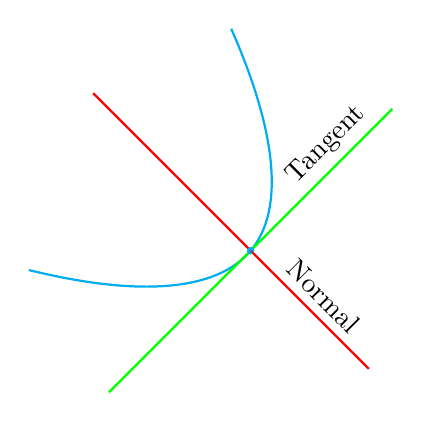
\begin{tikzpicture}[=>stealth]
\draw[thick,cyan,rotate=50](0,0)parabola(-2,2);
\draw[thick,cyan,rotate=50](0,0)parabola(2,2);
\draw[red,thick](1.5,-1.5)--(-2,2);
\draw[green,thick](-1.8,-1.8)--(1.8,1.8);
\draw(0,0)node[shape=circle,fill=cyan,scale=0.01cm]{};
\draw[red](0,0)--node[sloped,black,above]{Normal}(1.5,-1.5);
\draw[green](0.5,0.5)--node[sloped,black,above]{Tangent}(1.8,1.8);
\end{tikzpicture}
\end{figure}

The gradient of the normal to the equation $y = f(x)$ at $x_0$ is $\dfrac{-1}{f(x_0)}$. Therefore, the equation of the normal to the curve at $x_0$ is given by $$\boxed{y - f(x_0) = \frac{-1}{f(x_0)} (x - x_0)}$$
\end{solution}


\begin{exa}


Find the equation of the normal to the curve\hspace{0.2cm}$x^2 +3xy + y^2 = 5$\hspace{0.2cm} at $(1,1)$.
\end{exa}


\begin{solution}


$2x + 3y + 3x\dfrac{dy}{dx} + 2y\dfrac{dy}{dx} = 0$
$\implies\hspace{0.5cm} \dfrac{dy}{dx} = \dfrac{-(2x + 3y)}{3x + 2y}$


Thus, the gradient of the tangent at $(1,1)$ is $-1$. Then gradient of the normal to the curve at $(1,1)$ is $1$. There the equation of the normal to the curve at $(1,1)$ is $y - 1 = (x - 1)$
\end{solution}


\subsection{Limits}

\begin{defn}


Let $f:\mathbb{R}\longrightarrow \mathbb{R}$ be a given function and $c$ and $L$ be real numbers. Then $f(x)$ is said to tend to a limit $L$ as $x$ approaches $c$ if for any given $\varepsilon > 0 \hspace{0.2cm}\exists\hspace{0.2cm} \delta (\varepsilon) > 0 \ni$ whenever $0< \left|x - c\right|< \delta$, we have $\left|f(x) - L\right| < \varepsilon$.\\\\
\end{defn}

\begin{exa}


Use the definition of limits to show that $\hspace{0.3cm}\displaystyle{\lim\limits_{x\rightarrow 3} (5x - 2) = 13}$.
\end{exa}


\begin{proof}


We wish to show that given any $\varepsilon  > 0$, we can find a corresponding $\delta > 0 \ni \left|(5x -2) - 13\right| < \varepsilon$ whenever $\hspace{0.4cm} 0 < \left|x - 3\right| < \delta$.

\begin{align*}
\left|(5x - 2) - 13\right| & = \left|5x - 2 -13\right| = \left|5x - 15\right|\\
& =  5 \left|x - 3\right|
\end{align*}

Therefore, given any $\varepsilon > 0, \hspace{0.2cm} \exists \hspace{0.2cm} \delta (\varepsilon) = \dfrac{\varepsilon}{5}> 0 \ni$ whenever $0< \left|x - 3\right| < \delta$ we have 

\begin{align*}
\left|(5x - 2) - 13\right| & = 5\left|x - 3\right|\\
& < 5\delta = 5\Big(\dfrac{\varepsilon}{5}\Big)\\
& = \varepsilon
\end{align*}

Therefore, $\hspace{0.3cm}\displaystyle{\lim\limits_{x\rightarrow 3} (5x - 2) = 13}$
\end{proof}


\begin{note}
\begin{enumerate}
\item $\lim\limits_{x \rightarrow c} f(x) = L \iff$ given any $\varepsilon > 0 \hspace{0.2cm} \exists \hspace{0.2cm} \delta (\varepsilon) > 0 \ni \left|f(x) - L\right| < \varepsilon$\\ whenever $\hspace{0.3cm} 0 < \left|x - c\right| < \delta$

\item The definition implies that there can be at most one limit.

\item The inequality $\left|x - c\right| < \delta \implies c - \delta < x < c + \delta$. The part of the inequality which states that $0 < \left|x - c\right|, \hspace{0.3cm} x$ is not allowed to be equal to $c$.\\\\
\end{enumerate}
\end{note}

\begin{exa}


Prove that $\hspace{0.4cm} \lim\limits_{x \rightarrow 2} x^2 = 4$.
\end{exa}


\begin{solution}


$\displaystyle{\left|x^2 - 4\right| = \left|(x+2)(x-2)\right| = \left|x + 2\right|\hspace{0.1cm}\left|x - 2\right|}$\\

But $x$ lies between 1 and 3 i.e $1 < x < 3\hspace{0.3cm}$ i.e $\left|x - 2\right| < 1$.\\

Now $\left|x - 2\right| < 1 \iff 1 < x < 3$\\

$\implies \hspace{0.4cm} 2 < x + 1 < 4 \implies \left|x + 1\right| < 4$\\

$\forall \hspace{0.5cm} 1 < x < 3$


Thus $\hspace{0.2cm} \left|x^2 - 4\right| = \left|x + 2\right|\left|x -2\right| < 4\left|x - 2\right|$\\

Therefore, given any $\varepsilon > 0 \hspace{0.3cm} \exists \hspace{0.3cm} \delta(\varepsilon) = \dfrac{\varepsilon}{4}> 0$


$\exists\hspace{0.3cm} 0 < \left|x - 2\right| < \delta \implies \left|x^2 - 4\right|< 4\left|x - 2\right| < \delta$.\\

i.e $\hspace{0.3cm} \left|x^2 - 4\right| < \varepsilon \iff 0 < \left|x - 2\right| < \delta $\\

Therefore,  $\hspace{0.4cm} \lim\limits_{x \rightarrow 2} x^2 = 4$.
\end{solution}


\begin{exa}


Show directly from the definition of limits that $\hspace{0.3cm} \lim\limits_{x \rightarrow 5} \dfrac{1}{x - 1} = \dfrac{1}{4}$
\end{exa}


\begin{solution}
\begin{align*}
\left|f(x) - L\right| & = \left|\dfrac{1}{x - 1} - \dfrac{1}{4}\right| = \left|\dfrac{4 - (x - 1)}{4(x - 1)}\right| = \left|\dfrac{5 - x}{4(x - 1)}\right|\\\\
& = \dfrac{\left|x - 5\right|
}{4\left|x - 1\right|
}\\\\
& = \dfrac{1}{4}\hspace{0.1cm} \dfrac{1}{
\left|x - 1\right|}\hspace{0.1cm}\left|x - 5\right|
\end{align*}

$$4 < x < 6$$

Take $\left|x - 5\right| < 1 \iff 4 < x < 6$\\

$\implies\hspace{0.4cm} 3 < x - 1 < 5 \implies 3 < \left|x - 1\right|< 5$\\

$\implies\hspace{0.3cm} \dfrac{1}{5} < \dfrac{1}{\left|x - 1\right|
} < \dfrac{1}{3}$


$$\implies \hspace{0.5cm}\left|f(x) - L\right| = \left|\dfrac{1}{x - 1} - \dfrac{1}{4}\right| = \dfrac{1}{4}\hspace{0.1cm}\dfrac{1}{\left|x - 1\right|
}\hspace{0.1cm}\left|x - 5\right|<\dfrac{1}{4}\cdot\dfrac{1}{3}= \dfrac{1}{12}\hspace{0.1cm}\left|x -5\right|$$

$\implies\hspace{0.5cm} \left|\dfrac{1}{x - 1} - \dfrac{1}{4}\right| < \dfrac{1}{12}\hspace{0.1cm}\left|x - 5\right|$\\

Therefore, given any $\varepsilon > 0 \hspace{0.2cm} \exists \hspace{0.2cm} \delta (\varepsilon)  = 12\varepsilon \ni$ whenever $ 0 < \left|x - 5\right| < \delta$ we have 
$$\left|\dfrac{1}{x - 1}- \dfrac{1}{4}\right| < \dfrac{1}{12}\hspace{0.1cm}\left|x - 5\right| < \dfrac{1}{12}\delta = \frac{1}{12}(12\varepsilon) = \varepsilon$$

Therefore, $\hspace{0.3cm} \lim\limits_{x \rightarrow 5} \dfrac{1}{x - 1} = \dfrac{1}{4}$
\end{solution}


\subsection{Properties of Limits}

\begin{enumerate}
\item \textbf{Uniqueness of a limit}
Suppose $f(x) \longrightarrow L_1$ as $x \longrightarrow c$ and $f(x) \longrightarrow L_2$ as $x\longrightarrow c$. Then $L_1 = L_2$.

\item \textbf{Limit of a constant}
If $K$ is a constant and $f(x) = K\hspace{0.3cm} \forall$ values of $x$. Then for any number $c$, $\lim\limits_{x \rightarrow c} f(x) = K$

\item If $c$ is a real number and $f(x) = x$ then \hspace{0.2cm}$\displaystyle{\lim\limits_{x\rightarrow c} f(x) = c}$ 

\item \textbf{Limits of equal functions}
Suppose that there is a number $h>0$ such that $f(x) = g(x)\hspace{0.2cm} \forall x$ for which $\left|x - c\right| < h$. Suppose also that $\lim\limits_{x\rightarrow c} f(x) = L$, then $\lim\limits_{x\rightarrow c} g(x) = L$.

\item\textbf{Limit of a sum}
If $f$ and $g$ are two functions with $\lim\limits_{x\rightarrow c} f(x) = L_1$ and $\lim\limits_{x\rightarrow c} g(x) = L_2$ then\\ $\lim\limits_{x\rightarrow c} \Big[ f(x) + g(x)\Big] = L_1 +L_2$

\item \textbf{Limit of a product}
If $f$ and $g$ are two functions with $\lim\limits_{x\rightarrow c} f(x) = L_1$ and $\lim\limits_{x\rightarrow c} g(x) = L_2$ then\\ $\lim\limits_{x\rightarrow c} \big[f(x)\cdot g(x)\big] = L_1\cdot L_2$

\item \textbf{Limit of a quotient}
If $f$ and $g$ are two functions with $\lim\limits_{x\rightarrow c} f(x) = L_1$ and $\lim\limits_{x\rightarrow c} g(x) = L_2$, then \\ $\lim\limits_{x\rightarrow c}\dfrac{f(x)}{g(x)} = \dfrac{L_1}{L_2}$, provided $L_2\neq 0$

\item \textbf{Limit of a composite function}
Suppose that $f$ and $g$ are functions $b$ and $c$ are numbers $f(b)$ is defined and\\ $\lim\limits_{x\rightarrow c} f(x) = f(b),\hspace{0.3cm}\lim\limits_{x\rightarrow c} g(x) = b$. Then $\lim\limits_{x\rightarrow c} f\big[g(x)\big] = f(b)$

\item If $n$ is a positive integer and $c > 0$ then $\displaystyle{\lim\limits_{x\rightarrow c} \sqrt[n]{x} = \sqrt[n]{c}}$

\item If $n$ is positive integer, $L>0$ and $\lim\limits_{x\rightarrow c} f(x) = L$, then $\lim\limits_{x\rightarrow c} \sqrt[n]{f(x)} = \sqrt[n]{L}$
\end{enumerate}


\begin{exa}
Let $f(x) = \sqrt{2x^2 + 1}$ and $g(x) = 4x - 5$, find $\lim\limits_{x\rightarrow 2} f(g(x))$.
\end{exa}

\begin{solution}

Note that $\lim\limits_{x\rightarrow 2} \sqrt{2x^2 + 1} = 3$
\begin{align*}
\lim\limits_{x\rightarrow 2} f(4x - 5) & = \sqrt{2(4x - 5)^2 + 1} = \sqrt{2(3)^2 + 1}\\
& = \sqrt{19}
\end{align*}

$\lim\limits_{x\rightarrow 2} f(g(x)) = f(3)$

$f(3) = \sqrt{2(3)^2 + 1} = \sqrt{19}$

$\lim\limits_{x\rightarrow 2} f(g(x)) = f(3) = \sqrt{19}$
\end{solution}

\subsection{Limits at Infinity}
If $f$ is the function defined by $f(x) = \dfrac{1}{x}$ then 
\begin{enumerate}
\item $\lim\limits_{x\rightarrow +\infty} f(x) = 0$

\item $\lim\limits_{x\rightarrow -\infty} f(x) = 0$
\end{enumerate}

\begin{note}
\end{note}


The notation $x \longrightarrow +\infty$ is used if $x$ increases without bound through positive integers values and the notation $x \longrightarrow - \infty$ is used if $x$ decreases without bound through negative values.


The graph of $f(x) = \dfrac{1}{x}$ is as follows.

% DIAGRAM 22

\begin{figure}[H]
\centering
\begin{tikzpicture}[=>stealth]
\draw[-Stealth](-3,0)--(3,0)node[right]{$x$};
\draw[-Stealth](0,-3)--(0,3)node[above]{$y$};
\draw[smooth,thick,cyan, domain=0.1:2.5,variable=\x]plot(\x,{1/4*1/\x});
\draw[smooth,thick,cyan, domain=-2.5:-0.1,variable=\x]plot(\x,{1/4*1/\x});
\draw[thick,red](0,-2.5)--(0,2.5);
\draw[-Stealth](1,0.5)--(1.8,0.5);
\draw[-Stealth](-1.8,0.5)--(-1,0.5);
\draw(1,0.5)node[left]{$x$}
(1.8,0.5)node[right]{$0^+$}
(-1.8,0.5)node[left]{$x$}
(-1,0.5)node[right]{$0^-$}
(-0.2,0)node[below]{$0$};
\end{tikzpicture}
\end{figure}

$$\lim\limits_{x\rightarrow 0^+} \dfrac{1}{x} = +\infty\hspace{0.5cm}, \hspace{0.5cm} \lim\limits_{x\rightarrow 0^-} \dfrac{1}{x} = -\infty$$


\begin{exa}


Evaluate $\hspace{0.3cm}\lim\limits_{x\rightarrow +\infty} \dfrac{5x + 2}{3x - 7}$


\begin{align*}
\lim\limits_{x\rightarrow +\infty} \dfrac{5x + 2}{3x - 7} & = \lim\limits_{x\rightarrow +\infty} \dfrac{x\Bigl[5 + 2/x\Big]}{x\Big[3 - 7/x\Big]}\\
& = \frac{\lim\limits_{x\rightarrow +\infty}\Big[5 + 2 \Big(\dfrac{1}{x}\Big)\Big]}{ \lim\limits_{x\rightarrow +\infty}\Big[3 - 7\Big(\dfrac{1}{x}\Big)\Big]}\\
& = \dfrac{5}{3}\\
\end{align*}
\end{exa}

\begin{exa}


Evaluate $\lim\limits_{x\rightarrow +\infty} \dfrac{\sqrt[3]{x^3 + 1}}{5x - 2}\hspace{0.4cm},\hspace{0.4cm} x \neq \dfrac{2}{5}$
\end{exa}


\begin{solution}


$\lim\limits_{x\rightarrow +\infty} \dfrac{\sqrt[3]{x^3 + 1}}{5x - 2} = \dfrac{x \sqrt[3]{1 + \dfrac{1}{x^3}}}{x \Big[5 - 2\dfrac{1}{x}\Big]}= \dfrac{1}{5}$
\end{solution}


\subsection{Infinite Limits}
If $f(x)= \dfrac{1}{x}$, then $\lim\limits_{x \rightarrow ^+0} f(x) = + \infty$ and the $\lim\limits_{x \rightarrow 0^-} f(x)= -\infty$.


\begin{exa}


Find the $\lim\limits_{x \rightarrow 1} \dfrac{2}{(x - 1)^2}$

% DIAGRAM 23

\begin{figure}[H]
\centering
\begin{tikzpicture}[=>stealth]
\draw[-Stealth](-3,0)--(5,0)node[right]{$x$};
\draw[-Stealth](0,-1.5)--(0,3.5)node[above]{$y$};
\draw[red](1,-1)--(1,2.7);
\draw[smooth,thick,cyan,domain=1.5:4.5,variable=\x]plot(\x,{1/3*2/((\x-1)*(\x-1))});
\draw[smooth,thick,cyan,domain=-2.5:0.5,variable=\x]plot(\x,{1/3*2/((\x-1)*(\x-1))});
\draw(-0.2,0)node[below]{0}
(1,-1)node[below]{$x=1$}
(-2,0.5)node[left]{$x$}
(-1.2,0.5)node[right]{$1^-$}
(3.2,0.5)node[left]{$x$}
(4,0.5)node[right]{$1^+$};
\draw[-Stealth](-2,0.5)--(-1.2,0.5);
\draw[-Stealth](3.2,0.5)--(4,0.5);
\end{tikzpicture}
\end{figure}
\end{exa}

\begin{solution}


$\lim\limits_{x \rightarrow 1} \dfrac{2}{(x - 1)^2} = +\infty$
\end{solution}


\begin{exa}


Evaluate $\lim\limits_{x \rightarrow 3^+} \dfrac{1}{\sqrt{x - 3}}$

% DIAGRAM 24

\begin{figure}[H]
\centering
\begin{tikzpicture}[=>stealth]
\draw[-Stealth](0,0)--(7,0)node[right]{$x$};
\draw[-Stealth](2,-1)--(2,4)node[above]{$y$};
\draw[red](3,-1)--(3,3.2);
\draw[smooth,thick,cyan,domain=3.1:6.4,variable=\x]plot(\x,{1/sqrt(\x-3)});
\draw(3,-1)node[below,scale=0.9]{$x=3$}
(1.8,0)node[below,scale=0.8]{0}
(3.5,2)node[right]{$y=\dfrac{1}{\sqrt{x - 3}}$};
\draw[-Stealth](4,0.3)--(3.3,0.3);
\end{tikzpicture}
\end{figure}

$\lim\limits_{x \rightarrow 3^+} \dfrac{1}{\sqrt{x - 3}} = + \infty$
\end{exa}


\begin{note}
\end{note}


The function $f(x) = \dfrac{1}{\sqrt{x - 3}}$ is not defined for $x < 3$ and thus, $\lim\limits_{x\rightarrow 3^-}$ does not exist.


We have the following rules of operation
\begin{enumerate}
\item If $\lim\limits_{x\rightarrow c}f(x) = +\infty$ (or $-\infty$) and $\lim\limits_{x\rightarrow c}g(x) = b$ then $\lim\limits_{x\rightarrow c}\big[f(x) + g(x)\big]= + \infty$ or $(-\infty)$.

On the other hand if $\lim\limits_{x\rightarrow c}g(x) = -\infty$, nothing in general can be said about $$\lim\limits_{x\rightarrow c}\big[ f(x)+g(x)\big]$$ Further investigations of the particular limit will be necessary.

\item If $\lim\limits_{x\rightarrow c}f(x) = +\infty ($ or $-\infty)$ and  $\lim\limits_{x\rightarrow c}g(x) = b$, then 
\begin{enumerate}
     \item $\lim\limits_{x\rightarrow c}\big(f(x)\cdot g(x)\big) = +\infty ($ or $-\infty)$ if $b>0$.
     \item $\lim\limits_{x\rightarrow c}\big(f(x)\cdot g(x)\big) = -\infty ($ or $+\infty)$ if $b< 0$.
\end{enumerate}
 If $b = 0$, further investigations will be needed.

\item If $\lim\limits_{x\rightarrow c}f(x) = + \infty ($ or $-\infty)$ and $\lim\limits_{x\rightarrow c}g(x) = b$, then $\lim\limits_{x\rightarrow c}\dfrac{g(x)}{f(x)}=0$.

If $\lim\limits_{x\rightarrow c}g(x) = + \infty$, you may need to evaluate the limit using other methods.\
\end{enumerate}

\subsection{Indeterminate Forms of Limits}
Let  $f$ and $g$ be two functions having the property that $\lim\limits_{x\rightarrow c}f(x) = 0$ and $\lim\limits_{x\rightarrow c}g(x) =0$, then the function $\dfrac{f}{g}$ has the indeterminate form $\dfrac{0}{0}$ at $c$.


The rule for finding $\lim\limits_{x\rightarrow c}\dfrac{f(x)}{g(x)}$ in the case when $\dfrac{f}{g}$ has the indeterminate form $\dfrac{0}{0}$ is as follows:


If $\lim\limits_{x\rightarrow c}f(x) =0$ and $\lim\limits_{x\rightarrow c}g(x) = 0$, then $\lim\limits_{x\rightarrow c}\dfrac{f(x)}{g(x)} = \lim\limits_{x\rightarrow c}\dfrac{f'(x)}{g'(x)}$, when $f$ and $g$ are differentiable at $c$.


\begin{exa}


Find $\lim\limits_{x\rightarrow 1}\dfrac{x^3-5x^2 + 6x - 2 }{x^5 -3x^4 - 7x^2 + 9x}$
\end{exa}


\begin{solution}


Let $f(x) = x^3 - 5x^2 + 6x - 2\hspace{0.3cm}$ and $\hspace{0.4cm} g(x) = x^5 - 3x^4 - 7x^2 + 9$. Then $\lim\limits_{x\rightarrow 1}f(x) = f(1) = 0$. Also $\lim\limits_{x\rightarrow 1}g(x) = g(1) = 0$

\begin{align*}
\implies\hspace{0.5cm} \lim\limits_{x\rightarrow 1}\dfrac{f(x)}{g(x)}= & \lim\limits_{x\rightarrow 1}\dfrac{f'(x)}{g'(x)} = \dfrac{f'(1)}{g'(1)}\\
& = \dfrac{-1}{2}=\dfrac{1}{2}\\ 
\end{align*}

If $f$ and $g$ are two functions having the property that $\lim\limits_{x\rightarrow c}f(x) = \pm \infty$ and $\lim\limits_{x\rightarrow c}g(x) = \pm \infty$, then the function $\dfrac{f}{g}$ is said to be indeterminate form $\dfrac{\infty}{\infty}$. Thus,  $\lim\limits_{x\rightarrow c}\dfrac{f(x)}{g(x)} = \lim\limits_{x\rightarrow c}\dfrac{f'(x)}{g'(x)}$.
\end{solution}


\begin{exa}


Calculate $\hspace{0.3cm}\lim\limits_{x\rightarrow +\infty}\dfrac{e^x}{x}$.
\end{exa}


\begin{solution}


$\lim\limits_{x\rightarrow +\infty} e^x = + \infty$ and the $\lim\limits_{x\rightarrow +\infty}x = +\infty$.


$\implies \hspace{0.3cm} \lim\limits_{x\rightarrow +\infty}\dfrac{f(x)}{g(x)}$ is of indeterminate form $\Big(\dfrac{\infty}{\infty}\Big)$. Thus 
$$\lim\limits_{x\rightarrow +\infty}\dfrac{f(x)}{g(x)} = \lim\limits_{x\rightarrow +\infty}\dfrac{f'(x)}{g'(x)} = \lim\limits_{x\rightarrow +\infty}\frac{e^x}{1} = +\infty$$
\end{solution}


\begin{exa}


Evaluate the limit $\hspace{0.5cm}\lim\limits_{x\rightarrow 0} \dfrac{\cot x}{\cot 2x}$
\end{exa}


\begin{solution}


$\lim\limits_{x\rightarrow 0} \dfrac{\cot x}{\cot 2x}\hspace{1cm} \Bigg(\dfrac{\infty}{\infty}\Bigg)$

\begin{align*}
\lim\limits_{x\rightarrow 0} \dfrac{\cot x}{\cot 2x} & = \lim\limits_{x\rightarrow 0}\dfrac{-\csc^2x}{-2\csc^22x}\hspace{1cm} \dfrac{\infty}{\infty}
\end{align*}

$$\lim\limits_{x\rightarrow c}\dfrac{f(x)}{g(x)} = \lim\limits_{x\rightarrow c}\dfrac{f'(x)}{g'(x)}= \lim\limits_{x\rightarrow c}\dfrac{f''(x)}{g''(x)}=\lim\limits_{x\rightarrow 0}\dfrac{2\cot x \hspace{0.1cm}\csc x}{8\cot 2x\hspace{0.1cm}\csc 2x}$$

Note that at every stage of trying to find the limit we are getting the indeterminate form $\Big(\dfrac{\infty}{\infty}\Big)$. Thus, we may need to rewrite the limit as
\begin{align*}
\lim\limits_{x\rightarrow 0}\dfrac{\cot x}{\cot 2x} & = \lim\limits_{x\rightarrow 0}\dfrac{\dfrac{1}{\tan x}}{\dfrac{1}{\tan 2x}}\\\\
& = \lim\limits_{x\rightarrow 0}\dfrac{\tan 2x}{\tan x}\hspace{1cm} \Big(\dfrac{0}{0}\Big)\\\\
& = \lim\limits_{x\rightarrow 0}\dfrac{2\sec^22x}{\sec^2x}\\
& = \frac{2}{1}\\
& = 2\\
\end{align*}
\end{solution}

\subhead{Other examples of indeterminate forms}


Indeterminate types of the form $(0\cdot \infty)$ and $(\infty\hspace{0.2cm}-\infty)$


To evaluate the indeterminate forms of these types we have to express them in the types of the form $\dfrac{0}{0}$ or $\dfrac{\infty}{\infty}$.


\begin{exa}
Find
\begin{enumerate}
\item $\hspace{0.3cm}\lim\limits_{x\rightarrow \infty}x^2\cdot e^{-x}$
\item $\hspace{0.5cm}\lim\limits_{x\rightarrow 0} \Big(\csc x - \dfrac{1}{x}\Big)\hspace{1cm} (\infty- \infty)$

\begin{align*}
\lim\limits_{x\rightarrow 0} \Big(\csc x - \dfrac{1}{x}\Big) & = \lim\limits_{x\rightarrow 0}\Bigg[\dfrac{x - \sin x}{x\sin x}\Bigg]\hspace{1cm} \Bigg(\dfrac{0}{0}\Bigg)\\\\
& = \lim\limits_{x\rightarrow 0}\Bigg[\dfrac{1 - \cos x}{\sin x + x\cos x }\Bigg]\hspace{1cm} \Bigg(\frac{0}{0}\Bigg)\\\\
& = \lim\limits_{x\rightarrow 0}\Bigg[\frac{\sin x}{\cos x + \cos x - x \sin x}\Bigg]\\\\
& = \lim\limits_{x\rightarrow 0}\dfrac{\sin x}{2\cos x - x\sin}\\\\
& = \frac{0}{2} = 0\\
\end{align*}
\end{enumerate}
\end{exa}

\begin{solution}
$\hspace{0.3cm}\lim\limits_{x\rightarrow \infty}x^2\cdot e^{-x} \hspace{1cm}  (\infty \cdot 0)$
\begin{align*}
\lim\limits_{x\rightarrow \infty}x^2\cdot e^{-x} & = \lim\limits_{x\rightarrow \infty} \dfrac{x^2}{e^x}\hspace{1cm} \Big(\dfrac{\infty}{\infty}\Big)\\\\
& = \lim\limits_{x\rightarrow \infty}\dfrac{2x}{e^x}\hspace{1cm} \Big(\dfrac{\infty}{\infty}\Big)\\\\
& = \lim\limits_{x\rightarrow \infty} \dfrac{2}{e^x} = 0\\
\end{align*}
\end{solution}

\begin{exa}
\begin{enumerate}
\item $\hspace{0.4cm} \lim\limits_{x\rightarrow 0} x \csc x\hspace{1cm} (0\cdot\infty)$

\begin{align*}
\lim\limits_{x\rightarrow 0} x \csc x & = \lim\limits_{x\rightarrow 0} x \cdot \dfrac{1}{x}\\\\
& = \lim\limits_{x\rightarrow 0}\frac{x}{\sin x}\hspace{1cm} \dfrac{0}{0}\\\\
& = \lim\limits_{x\rightarrow 0} \frac{1}{\cos x}\\
&= 1\\
\end{align*}

\item $\lim\limits_{x\rightarrow 1}\Bigg[\dfrac{1}{\ln x} - \dfrac{x}{x - 1}\Bigg]\hspace{1cm} (\infty - \infty)$

\begin{align*}
\lim\limits_{x\rightarrow 1}\Bigg[\dfrac{1}{\ln x} - \dfrac{x}{x - 1}\Bigg] & = \lim\limits_{x\rightarrow 1}\dfrac{(x - 1)- x \ln x}{(x-1)\ln x}\hspace{1cm} \text{L'Hopital's rule}\hspace{0.2cm} \dfrac{0}{0}\hspace{0.2cm} \text{or}\hspace{0.2cm} \dfrac{\infty}{\infty}\\\\
& = \lim\limits_{x\rightarrow 1}\dfrac{1- (\ln x + 1)}{\ln x + \dfrac {x-1}{x}}\\\\
& = \lim\limits_{x\rightarrow 1} \frac{-\ln x}{\ln x + 1 - \dfrac{1}{x}}\hspace{1cm} \dfrac{0}{0}\\\\
& = \lim\limits_{x\rightarrow 1}\hspace{0.1cm} \dfrac{\dfrac{-1}{x}}{\dfrac{1}{x} + \dfrac{1}{x^2}}\\\
& = \frac{-1}{2}\\\\
\end{align*}
\end{enumerate}
\end{exa}

\subsubsection{Indeterminate types of the form $0^0$, $\infty^0$ and $1^{\infty}$}
In these forms we use the fact that if $\lim y$ is one of the types above,
then $\lim (\ln y)$ is of the type $0\cdot \infty$, which has already been
treated.


\begin{exa}
Evaluate
\begin{enumerate}
\item $\hspace{0.5cm}  \lim\limits_{x\rightarrow 0} \Bigg(1 + \dfrac{1}{x}\Bigg)^x\hspace{2cm} (\infty^0)$
\item $\hspace{0.5cm}  \lim\limits_{x\rightarrow \infty} \Big(1 + \dfrac{1}{x}\Big)^x\hspace{2cm} \big(1^{\infty}\big)$

Let $\hspace{0.3cm} L = \lim\limits_{x\rightarrow \infty} \Big(1 + \dfrac{1}{x}\Big)^x$ Then
\begin{align*}
\ln L & = \ln \Bigg[\lim\limits_{x\rightarrow \infty} \Big(1 + \dfrac{1}{x}\Big)^x\Bigg]\\
& = \lim\limits_{x\rightarrow \infty}\Bigg[\ln \Big(1 + \dfrac{1}{x}\Big)^x\Bigg]\\
& = \lim\limits_{x\rightarrow \infty}\Bigg[x \ln \Big(1 + \dfrac{1}{x}\Big)\Bigg]\\
& = \lim\limits_{x\rightarrow \infty}\dfrac{\ln\Big( 1 + \dfrac{1}{x}\Big)}{\dfrac{1}{x}}\hspace{2cm} \dfrac{0}{0}\\\\
& = \lim\limits_{x\rightarrow \infty}\hspace{0.1cm} \frac{\dfrac{1}{1 + \dfrac{1}{x}}\Big(-\dfrac{1}{x^2}\Big)}{\Big(-\dfrac{1}{x^2}\Big)}=\lim\limits_{x\rightarrow \infty}\hspace{0.1cm} \dfrac{1}{1 + \dfrac{1}{x}}\\\\
& = 1\\
\end{align*}

$$\implies\hspace{0.5cm} \ln L = 1 \hspace{0.5cm} \implies\hspace{0.5cm} L = e^1 = e$$
\end{enumerate}
\end{exa}

\begin{solution}
Let $\hspace{0.5cm}y = \lim\limits_{x\rightarrow 0} \Bigg(1 + \dfrac{1}{x}\Bigg)^x$ Then

\begin{align*}
\ln y & = \ln \Bigg[\lim\limits_{x\rightarrow 0} \Big(1 + \dfrac{1}{x}\Big)^x\Bigg]
 = \lim\limits_{x\rightarrow 0}\Bigg[\ln \Big(1 + \dfrac{1}{x}\Big)^x\Bigg]\\\\
 & = \lim\limits_{x\rightarrow 0}\Bigg[ x \ln \Big(1 + \dfrac{1}{x}\Big)^x\Bigg]\hspace{2cm} (0\cdot \infty)\\\\
& = \lim\limits_{x\rightarrow 0}\hspace{0.1cm} \dfrac{\ln \Big( 1 + \dfrac{1}{x}\Big)}{\dfrac{1}{x}}\hspace{2cm} \dfrac{\infty}{\infty} 
\end{align*} 
\begin{align*} 
 \ln y & = \lim\limits_{x\rightarrow 0}\hspace{0.1cm} \dfrac{\dfrac{1}{1 + 1/x} \Big(-\dfrac{1}{x^2}\Big)}{\Big(-\dfrac{1}{x^2}\Big)}= \lim\limits_{x\rightarrow 0} \hspace{0.1cm}\dfrac{1}{1 + \dfrac{1}{x}}\\
 & = 0
\end{align*}

$$\implies\hspace{0.5cm} \ln y = 0\hspace{0.4cm} \implies \hspace{0.4cm} y = e^0 = 1$$

$\therefore\hspace{0.5cm}  \lim\limits_{x\rightarrow 0} \Big(1 + \dfrac{1}{x}\Big)^x = 1$
\end{solution}

\pagebreak
\subsection{Continuity of a Function}
Let $f$ be defined for all $x$ near $x = x_0$ as well as at $x = x_0$ (i.e in a $\delta - $ neighborhood of $x_0$). The function $f$ is said to be continuous at $x = x_0$ if $$\boxed{\lim\limits_{x \rightarrow x_0} f(x) = f(x_0)}$$

Note that this implies three conditions which must be met in order that $f(x)$ be continuous at $x = x_0$
\begin{enumerate}
\item $\lim\limits_{x \rightarrow x_0} f(x)$ exists i.e $\lim\limits_{x \rightarrow x_0} f(x) = L \in \mathbb{R}$.
\item $f(x_0)$ must exist if $f(x)$ is defined at $x = x_0$.
\item $\displaystyle{\lim\limits_{x \rightarrow x_0} f(x) = f(x_0)}$
\end{enumerate}

Equivalently, if $f$ is continuous at $x_0$ , we can write this in the suggestive form $$\lim_{x \rightarrow x_0} f(x) = f\Big(\lim\limits_{x \rightarrow x_0} x\Big)$$


\begin{exa}
\begin{enumerate}
\item Determine whether $f(x) = 
\begin{cases} 
x^2, & x \neq 2\\
0, & x = 2\\
\end{cases}
$ is continuous at $x = 2$.

% DIAGRAM 25

\begin{figure}[H]
\centering
\begin{tikzpicture}[=>stealth]
\draw[-Stealth](-3,0)--(3,0)node[right]{$x$};
\draw[-Stealth](0,-0.5)--(0,3)node[above]{$y$};
\draw(1.5,1.125)node[shape=circle,thick,scale=0.01cm, draw=cyan]{};
\draw[smooth,domain=0:1.49,thick,cyan,variable=\x]plot(\x,1/2*\x*\x);
\draw[smooth,domain=1.51:2,thick,cyan,variable=\x]plot(\x,1/2*\x*\x);
\draw[smooth,domain=-2:0,thick,cyan,variable=\x]plot(\x,1/2*\x*\x);
\draw(1.5,0.05)--(1.5,-0.05);
\draw(1.5,-0.01)node[below]{2};
\end{tikzpicture}
\end{figure}

\begin{enumerate}
\item $\displaystyle{\lim_{x\rightarrow 2^-} f(x ) = \lim_{x\rightarrow 2}x^2 = 4}$

$\displaystyle{\lim_{x\rightarrow 2^+}f(x) = \lim_{x\rightarrow 2}x^2 = 4 = \lim_{x\rightarrow 2^-}f(x)}$

$\therefore\hspace{0.3cm} \lim\limits_{x \rightarrow 2}f(x)$ exists.

\item $f(x) = f(2) = 0$

\item $f(2) \neq \lim\limits_{x\rightarrow 2} f(x)$

$\therefore\hspace{0.2cm} f$ is not continuous at $x = 2$.
\end{enumerate}

\item Determine if $f(x) = x^2\hspace{0.2cm} \forall x \in \mathbb{R}$ is continuous at $x = 2$.

$$\lim_{x\rightarrow 2} f(x) = \lim_{x\rightarrow 2}x^2 = f(2)  = 4$$
$\therefore\hspace{0.2cm}f$ is continuous at $x = 2$.
\end{enumerate}

Points where $f$ fails to be continuous are called discontinuities of $f$ and $f$ is said to be discontinuous at these points.


Alternatively, if for any $\varepsilon > 0$ we can find $\delta > 0 \ni \left|f(x) - f(x_0)\right| < \varepsilon$ whenever $\left|x - x_0\right| < \delta$, then $f$ is continuous at $x = x_0$ provided $f(x_0)$ exists.\\\\
\end{exa}

\subsubsection{Right and Left $-$ hand continuity}
If $f$ is defined only for $x\geq x_0$, the above definition does not apply. In such case we call $f$ continuous on the right at $x = x_0$ if $\displaystyle{\lim\limits_{x \rightarrow x_0^+}f(x) = f(x_0)}$.


Similar definition exists for left continuity.


\subsubsection{Continuity in an Interval}
A function $f$ is said to be continuous in an interval if it is continuous at all points of the interval. In particular, if $f$ is defined in a closed interval $a \leq x \leq b$ or $[a,b]$, then $f$ is continuous in the interval if and only if $$\displaystyle{\lim_{x \rightarrow x_0} f(x) = f(x_0)}$$ or $a< x_0 < b,$ $\hspace{0.4cm} \displaystyle{\lim_{x \rightarrow x_a^+} f(x) = f(a)}$ and $\displaystyle{\lim_{x \rightarrow b^-} f(x) = f(b)}$.


\subsubsection{Theorems on Continuity}

\begin{thm}


If $f$ and $g$ are continuous at $x = x_0$, so also are the functions $f(x) \pm g(x) \hspace{0.2cm} , \hspace{0.2cm} f(x)\cdot g(x) \hspace{0.2cm}$ and $\dfrac{f(x)}{g(x)}$, the last one only if $g(x_0) \neq 0$.
\end{thm}


\begin{thm}


Functions described as follows are continuous in every finite interval
\begin{enumerate}
\item all polynomials
\item $\sin x $ and $\cos x$
\item $a^x,\hspace{0.2cm} x>0$
\end{enumerate}
\end{thm}

\begin{thm}


Let the function $f$ be continuous at $x = x_0$. Also, suppose that a function $g$, represented by $z = g(y)$, is continuous at $y_0$, where $y = f(x)$. Then the composite function represented by $z = g[f(x)]$ is also continuous at $x = x_0$. $[$ one can say that a continuous function of a continuous is continuous$]$.
\end{thm}


\begin{thm}


If $f(x)$ is continuous in a closed interval, it is bounded in the interval.
\end{thm}


\begin{thm}


If $f(x)$ is continuous at $x = x_0$ and $f(x_0) > 0$ $[$ or $f(x_0)< 0]$, there exists an interval about $x = x_0$, in which $f(x_0) > 0$ $\hspace{0.2cm}[$ or $f(x)< 0]$.
\end{thm}


\begin{thm}


If a function $f(x)$ is continuous in the interval and is either strictly increasing or strictly decreasing, the inverse function $f^{-1}(x)$ is single$-$valued, continuous, and either strictly increasing or strictly decreasing.
\end{thm}


\begin{thm}


If $f(x)$ is continuous in $[a,b]$ and if $f(a) = A$ and $f(b) = B$, then corresponding to any number $c$ between $A$ and $B$, there exists, atleast one number $c$ in $[a,b]$ such that $f(c)= c$. This is  called the intermediate value theorem.
\end{thm}


\begin{thm}


If $f(x)$ is continuous in $[a,b]$ and $f(a)$ and $f(b)$ have opposite signs, there is atleast one $c$ for which $f(c) = 0$ where $a< c<b$. This is related to theorem 7.
\end{thm}


\subsubsection{Piece-wise Continuity}
A function is called piece-wise continuous in an interval $a\leq x \leq b$ if the interval can be subdivided into a finite numbers of intervals in each of which the function is continuous and has finite left-hand and right-hand limits.

% DIAGRAM 26

\begin{figure}[H]
\centering
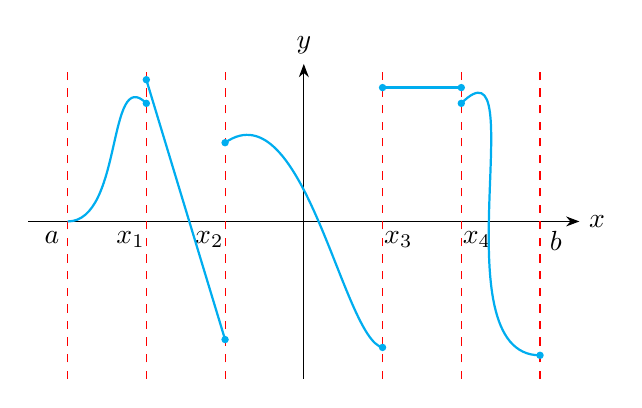
\begin{tikzpicture}[=>stealth]
\draw[-Stealth](-3.5,0)--(3.5,0)node[right]{$x$};
\draw[-Stealth](0,-2)--(0,2)node[above]{$y$};
\draw[red,dashed](-3,-2)--(-3,2)
(-2,-2)--(-2,2)
(-1,-2)--(-1,2)
(1,-2)--(1,2)
(2,-2)--(2,2)
(3,-2)--(3,2);
\draw(-3.2,0)node[below]{$a$}
(-2.2,0)node[below]{$x_1$}
(-1.2,0)node[below]{$x_2$}
(1.2,0)node[below]{$x_3$}
(2.2,0)node[below]{$x_4$}
(3.2,0)node[below]{$b$}
(1,1.7)node[shape=circle,fill=cyan,scale=0.01cm]{}
(2,1.7)node[shape=circle,fill=cyan,scale=0.01cm]{}
(-2,1.8)node[shape=circle,fill=cyan,scale=0.01cm]{}
(-1,-1.5)node[shape=circle,fill=cyan,scale=0.01cm]{}
(-1,1)node[shape=circle,fill=cyan,scale=0.01cm]{}
(1,-1.6)node[shape=circle,fill=cyan,scale=0.01cm]{}
(-2,1.5)node[shape=circle,fill=cyan,scale=0.01cm]{}
(2,1.5)node[shape=circle,fill=cyan,scale=0.01cm]{}
(3,-1.7)node[shape=circle,fill=cyan,scale=0.01cm]{};
\draw[thick,cyan](1,1.7)--(2,1.7);
\draw[thick,cyan](-2,1.8)--(-1,-1.5);
\draw[thick,cyan](-1,1)..controls(0,1.7)and(0.5,-1.5)..(1,-1.6);
\draw[thick,cyan,out=0](-3,0)to(-2,1.5);
\draw[thick,cyan,in=180](2,1.5)to(3,-1.7);
\end{tikzpicture}
\end{figure}

\vspace{1cm}

\begin{exa}
\begin{enumerate}
\item Prove that $f(x) = x$ is continuous at any point $x = x_0$.
\item Prove that $f(x) = 2x^3 + x$ is continuous at any point $x = x_0$.
\item For what values of $x$ is the function discontinuous $$ f(x) = \frac{x - |x|}{x}$$
\item $\displaystyle{ g(x) = 
\begin{cases}
\dfrac{x - |x|}{x}, & x < 0\\\\
2, & x = 0\\
\end{cases}}\hspace{0.3cm}$ is $g$ continuous for $x \leq 0$?\\\\
\end{enumerate}
\end{exa}

\begin{solution}
\subhead{Part 1}
We need to show that given any $\varepsilon > 0, \exists $ a $\delta > 0\ni \left|f(x) - f(x_0)\right| < \varepsilon $\\ whenever $0<\left|x - x_0\right|< \delta$.\\
Now given $f(x) = x$, then $\left|f(x) - f(x_0)\right| = \left|x - x_0\right| < \varepsilon = \delta $. So by choosing $\delta = \varepsilon $ we have the result, since $f(x_0) = x_0$.\\

\subhead{Part 2}
Since $g(x) = x$ is continuous at any point $x = x_0$, then by theorem 3, $h(x) = x\cdot x = x^2$ is continuous and $K(x) = x^2\cdot x = x^3$ is also continuous. Similarly, $M(x) = 2x^3$ is continuous.

$\therefore\hspace{0.3cm} f(x) = M(x) + g(x) = 2x^3 + x$ is continuous by theorem 3.

\subhead{Part 3}
For $x> 0$, $\hspace{0.2cm} f(x) = \dfrac{x - x}{x} =  0$ discontinuous.

For $x< 0,\hspace{0.2cm} f(x) = \dfrac{x - (-x)}{x} = 2$ continuous.

For $x = 0$, $\hspace{0.2cm} f(x)$ is undefined. Therefore, $f$ is discontinuous only at $x = 0$.

\subhead{Part 4}
\begin{enumerate}
       \item For $x< 0\hspace{0.3cm} g(x) = \dfrac{x - |x|}{x} = 2$ and is continuous for $x<0$.

       \item $g(0) = 2$

       \item $\displaystyle{\lim\limits_{x \rightarrow 0^-} g(x) = \lim\limits_{x \rightarrow 0^-} \dfrac{x - |x|}{x} = 2 = g(0)}$
\end{enumerate}
\end{solution}

\pagebreak
\subsection{Mean Value Theorems}
The mean value theorem (MVT) is used to prove important concepts in differential calculus.


\subsubsection{Rolle's Theorem}
Let $f$ be continuous on the close interval $[a,b]$ and differentiable on the open interval $(a,b)$. If $f(a) = f(b)$ then $\exists$ at least one number $c \in (a,b)$ at which $f'(c) = 0$.

% DIAGRAM 27

\begin{figure}[H]
\centering
\begin{tikzpicture}[=>stealth]
\draw[-Stealth](-2.5,-2)--(2.5,-2)node[right]{$x$};
\draw[-stealth](-0.7,-3.5)--(-0.7,1)node[above]{$y$};
\draw[smooth,domain=-1.8:1.8,thick, cyan, variable=\x]plot(\x,-\x*\x)node[black, right]{$y = f(x)$};
\draw[thick,red,dashed](0,0)--(0,-2);
\draw(1.4,-2.05)--(1.4,-1.95)
(-1.4,-2.05)--(-1.4,-1.95);
\draw(0,-2)node[below]{c}
(1.4,-2)node[below]{$b$}
(-1.4,-2)node[below]{$a$};
\end{tikzpicture}
\end{figure}

\begin{exa}


Let $f(x) = (x - 1)(x - 2)$. Then $f(1) = f(2) = 0 \hspace{0.2cm}\exists $ a point $c\in (1,2)\ni f'(c) = 0$.


\begin{note}
$f(x) = (x - 1) (x - 2) = x^2 - 3x + 2$
\end{note}


$f'(x)  = 2x - 3$


$f'(c)  = 2c - 3 = 0$

$$\implies\hspace{0.5cm} c = \frac{3}{2}\in (1,0)$$
\end{exa}


\subsubsection{Mean Value Theorem}
Let $f$ be a continuous on a closed interval $[a,b]$ and differentiable on the open interval $(a,b)$. Then $\exists$ at least one number $c\in (a,b)$ such that $$f'(c) = \frac{f(b) - f(a)}{b - a}$$

% DIAGRAM 28
\begin{figure}[H]
\centering
\begin{tikzpicture}[=>stealth]
\draw[-Stealth](-3,-2)--(7,-2)node[right]{$x$};
\draw[-Stealth](0.5,-2.5)--(0.5,2.5)node[above]{$y$};
\draw[smooth,thick,cyan,domain=-0.75:6.5,variable=\x,]plot(\x,{1.5*sin((\x)r)})node[above,black]{$y=f(x)$};
\draw(1.6,1.5)node[shape=circle,fill=cyan,scale=0.01cm,draw=cyan]{}
(-0.2,-0.3)node[shape=circle,fill=cyan,scale=0.01cm,draw=cyan]{}
(2.7,0.63)node[shape=circle,fill=cyan,scale=0.01cm,draw=cyan]{};
\draw[red](-0.18,-0.3)--(2.7,0.63);
\draw[dashed,red](-0.2,-2)--(-0.2,-0.28)
(2.7,-2)--(2.7,0.6)
(1.6,-2)--(1.6,1.4);
\draw(-0.2,-0.3)node[left]{$(a,f(a))$}
(2.7,0.63)node[right]{$(b,f(b))$}
(2.7,-2)node[below]{$b$}
(1.6,-2)node[below]{$c$}
(-0.2,-2)node[below]{$a$};
\end{tikzpicture}
\end{figure}

\vspace{0.5cm}

\begin{exa}


Let $f(x) = x^2\hspace{0.2cm} , \hspace{0.2cm} a = 2$ and $b = 5$. Then $$\frac{f(b) - f(a)}{b - a}  = \frac{f(5) - f(2)}{5 - 2} = 7$$ Since $f$ is continuous in the closed interval $[2,5]$, and differentiable in the open interval $(2,5)$ by the (MVT) $\exists$ at least one point $c \in (2,5)$ such that $$f'(c) = 7$$
Now, $f'(x) = 2x$


$\implies \hspace{0.5cm} f'(c) = 2c = 7 \implies c = \frac{7}{2}\in (2,5)$.

% DIAGRAM 29

\begin{figure}[H]
\centering
\begin{tikzpicture}[=>stealth]
\draw[-Stealth](0,-1)--(0,4)node[above]{$y$};
\draw[-Stealth](-3,0)--(3,0)node[right]{$x$};
\draw[smooth,thick, cyan, domain=-2.5:2.5, variable=\x]plot(\x,1/2*\x*\x)node[black,right]{$y = x^2$};
\draw[thick,red](1,0.5)--(2.3,2.645);
\draw[dashed,red](1,0)--(1,0.5)
(2.3,0)--(2.3,2.645)
(1.65,0)--(1.65,1.361);
\draw(1,0.5)node[left,scale=0.8]{(2,4)}
(2.3,2.645)node[left,scale=0.8]{(5,25)}
(1,0)node[below,scale=0.8]{2}
(1.65,0)node[below]{$\frac{7}{2}$}
(2.3,0)node[below,scale=0.8]{5};
\end{tikzpicture}
\end{figure}

The mean $-$ value theorem can be put in so many useful forms.


For example multiplying through by $(b - a)$ yields, $$f(b) = f(a) + (b - a) f'(c)\hspace{0.2cm} , \hspace{0.2cm} c \in (a,b)$$

A single replacement of $b$ by $x$ yields $$f(x) = f(a) + (x - a) f'(c)\hspace{0.2cm}, \hspace{0.2cm} c \in (a, x)$$
\end{exa}


\begin{exa}


Use the mean value theorem to approximate $\sqrt[6]{65}$.
\end{exa}


\begin{solution}


Let $f(x) = \sqrt[6]{x}\hspace{0.3cm}$ i.e $\hspace{0.3cm} f(x) = x^{1/6}$.


Then we take $a = 64$ and $b = 65$. Now, note that the this function is continuous on the closed interval $[64,65]$ and is differentiable in open interval $(64,65)$. 
$$f'(x) = \frac{1}{6}x^{-5/6}$$

Applying (MVT) we have
$$f(65) = f(64) + (65 - 64)f'(c)\hspace{0.2cm}, \hspace{0.2cm} c \in (64,65)$$ 

$$f(65) = f(64) + (65 - 64)\Big(\frac{1}{6}c^{-5/6}\Big)$$

We approximate $c = 64$.

\begin{align*}
\text{Thus}\hspace{0.5cm} \sqrt[6]{65} & = \sqrt[6]{64} + 1 \times \frac{1}{6}\Big( 64^{1/6}\Big)^{-5}\\
& = 2 + \frac{1}{6} \times 2^{-5}\\
& = 2 + \frac{1}{6}\times \frac{1}{32}\\
& = 2.00521\\
\end{align*}
\end{solution}

\begin{exa}


Use the mean value theorem to show that $\hspace{0.2cm} \sin x < x\hspace{0.2cm}$ for $x>0$.
\end{exa}


\begin{proof}


Recall that $\sin x \leq 1 \hspace{0.2cm} \forall x \in \mathbb{R}$. Thus, it is obvious that $\sin x <x$ when $x> 1.$


Now we consider the case where $0< x \leq 1$. Let us take $f(x) = \sin x $ with $a = 0$ and $b = 1$ and applying the formula $$f(x) = f(a) + (x - a) f'(c)\hspace{0.3cm},\hspace{0.3cm} c\in (0, x)\hspace{0.3cm} \cdots\cdots\cdots\hspace{0.3cm} (I)$$
$$f'(x) = \cos x \implies f'(c) = \cos c$$
Thus, using $(I)$ we have $$\sin x = \sin 0 + (x -0) \cos c = x\cos c \hspace{0.3cm} , \hspace{0.3cm} c \in (0,x)$$
$$\text{i.e}\hspace{0.3cm} \sin x = x \cos c$$
Since $0 < c < x \leq 1, \hspace{0.3cm} \cos c < 1$ thus, $x\cos c < x$. Therefore, $\sin x < x$. $$\implies \hspace{0.2cm} \sin x < x\hspace{0.3cm} \forall x > 0.$$
\end{proof}


\subsubsection{Generalized Mean Value Theorem}
If $f(x)$ and $g(x)$ are continuous on the closed interval $[a,b]$ and if $f'(x)$ and $g'(x)$ exist and $g'(x) = 0$ everywhere on the interval except possibly at the end points, then $\exists$ at least one point $c\in (a,b) \ni$ $$\frac{f(b) - f(a)}{g(b) - g(a)} = \frac{f'(c)}{g'(c)}\hspace{0.3cm} \cdots\cdots\cdots\hspace{0.3cm} (II)$$
Note that for the case $g(x) = x$, then the theorem becomes the MVT.


\subsubsection{Extended Mean Value Theorem}
If $f(x)$ and its $(n-1)$ derivatives are continuous on the closed interval $[a,b]$, and if $f^n(x)$ exists everywhere on the interval except possibly at the end points, then $\exists$ atleast on point $c\in (a,b) \ni$
$$f(b) = f(a) + \frac{f'(a)}{1!}(b - a) + \frac{f''(a)}{2!}(b - a)^2 + \cdots\cdots + \frac{f^{(n-1)(a)}}{(n-1)!}(b - a)^{n-1} + \frac{f^n(a)}{n!}(b - a)^n\hspace{0.3cm}\cdots\cdots\hspace{0.2cm} (III)$$

$(III)$ is called the Taylor's formula with the remainder $$R_n = \frac{f^n(a) (b - a)^n}{n!}$$ when $b$ is replaced with the variable $x$, $(III)$ becomes
$$f(x) = f(a) + \frac{f'(a)}{1!}(x - a) + \frac{f''(a)}{2!}(x - a)^2 + \cdots\cdots + \frac{f^{(n-1)(a)}}{(n-1)!}(x - a)^{n-1} + \frac{f^n(a)}{n!}(x - a)^n\hspace{0.3cm}\cdots\cdots\hspace{0.2cm} (IV)$$
for some $c \in (a,x)$.


$(IV)$ is called the Taylor's series with the remainder  $$R_n(x) = \frac{f^n(a) (x - a)^n}{n!}$$


When $(a)$ is replaced by 0 in $(IV)$ we have the Maclaurin's series with the remainder $$R_n(x) = \frac{f^n(0) (x )^n}{n!}$$

i.e
$$f(x) = f(0) + \frac{f'(0)}{1!}x  + \frac{f''(0)}{2!}x^2 + \cdots\cdots\cdots + \frac{f^{(n-1)(0)}}{(n-1)!}x^{n-1} + \frac{f^n(a)}{n!}x^n$$

Note that $\displaystyle{R_n(x) = \frac{f^n(0)}{n!}x^n}$ is a function of $x$.


\subsection{Series}

A series is what results from adding the terms of a sequence. The central
question is whether an infinite sum of this kind has a finite value at all, and
it is not settled by the terms merely shrinking: the terms of the harmonic
series tend to zero while its sum grows without bound.

The subsections below build the answer in order. Sequences come first, since a
series is defined as the limit of its sequence of partial sums. The convergence
tests follow --- each a different way of comparing an unfamiliar series with one
whose behaviour is known. Power series then reverse the question: instead of
asking whether a given series converges, they treat the sum as a function of $x$
and ask where it is defined, which leads to the representation of familiar
functions as infinite polynomials.


\subsection{Infinite Sequences}

\begin{defn}


An infinite sequence $\{a_n\}^{\infty}_{n=1} = a_1, a_2,\cdots\cdots\cdots\hspace{0.3cm}$ is a function on $n$ whose domain is the set of positive integers.
\end{defn}


\begin{defn}


A sequence is bounded if $\exists$ numbers, $p$ and $q$ $\ni p \leq a_n \leq q \hspace{0.2cm}\forall$ values of $n\in \mathbb{Z}^+$.
\end{defn}


\begin{exa}


The sequence $\{a_n\}^{\infty}_{n=1} = \dfrac{3}{2}, \dfrac{5}{4},\dfrac{7}{6}, \cdots\cdots\cdots, \dfrac{2n+ 1}{2n}$, is bounded since, $\hspace{0.2cm} \forall n \in \mathbb{Z}^+\hspace{0.4cm} 1 \leq a_n \leq 2$.
\end{exa}


\begin{defn}


A sequence $\{a_n\}^{\infty}_{n=1}$ is said to be increasing if $\hspace{0.4cm} a_1\leq a_2\leq a_3\cdots\cdots\cdots \leq a_n \leq \cdots\cdots$


A sequence is decreasing if $\hspace{0.4cm} a_1\geq a_2\geq a_3\cdots\cdots\cdots \geq a_n \geq \cdots\cdots$
\end{defn}


\begin{defn}


A sequence $\{a_n\}^{\infty}_{n=1}$ is said to converge to a finite number $a$ if $\hspace{0.4cm} \lim\limits_{n\rightarrow \infty} a_n = a$.


A sequence which converges is called a convergent sequence otherwise it is a divergent sequence.
\end{defn}


\subhead{Some Properties of Sequences}
\begin{enumerate}
\item Every bounded increasing sequence (or decreasing sequence) converges.
\item Every unbounded sequence diverges.
\item A convergent (divergent) sequence remains convergent (divergent) after any or all its terms altered.
\item Let $\lim\limits_{n \rightarrow \infty} a_n = a$ and $\lim\limits_{n \rightarrow \infty} b_n = b$
\begin{enumerate}
     \item $\lim\limits_{n \rightarrow \infty} K a_n = Ka$

     \item $\lim\limits_{n \rightarrow \infty}( a_n\pm b_n) = \lim\limits_{n \rightarrow \infty} a_n  \pm \lim\limits_{n \rightarrow \infty} b_n  = a \pm b$

     \item $\lim\limits_{n \rightarrow \infty} (a_n\cdot b_n) = \lim\limits_{n \rightarrow \infty} a_n \cdot \lim\limits_{n \rightarrow \infty} b_n = a\cdot$

     \item $\lim\limits_{n \rightarrow \infty} \dfrac{a_n}{b_n} = \dfrac{ \lim\limits_{n \rightarrow \infty} a_n}{\lim\limits_{n \rightarrow \infty} b_n} = \dfrac{a}{b}$ provided $b \neq 0$.
\end{enumerate}

\item If $\{a_n\}^{\infty}_{n=1}$ is a sequence of nonzero terms and if $\lim\limits_{n \rightarrow \infty} a_n = \infty$ then $\lim\limits_{n \rightarrow \infty}\dfrac{1}{a_n} = 0$

\item If $r>1$, then $\lim\limits_{n \rightarrow \infty} r^n = +\infty$

\item If $|r|<1$, then $\lim\limits_{n \rightarrow \infty} r^n = 0$
\end{enumerate}

\begin{exa}


Let a sequence be $\Big\{\Big(\dfrac{1}{2}\Big)^n\Big\}$. Then $\lim\limits_{n \rightarrow \infty} \Bigg(\dfrac{1}{2}\Bigg)^n = 0$.
\end{exa}


\subsection{Infinite Series}

\begin{defn}


Let $\{a_n\}^{\infty}_{n=1}$ be an infinite sequence. An infinite is given by $$\sum^{\infty}_{n=1}a_n = a_1 + a_2 + \cdots\cdots\cdots$$

The partial sums of the series are given $$S_1 = a_1\hspace{0.2cm} , \hspace{0.2cm} S_2 = a_1 + a_2\hspace{0.2cm} , \hspace{0.2cm} S_3 = a_1 + a_2 + a_3\hspace{0.3cm} \cdots\cdots\cdots\hspace{0.3cm} S_N = a_1 + a_2 + \cdots\cdots a_N = \sum^n_{n=1}$$

Now $\displaystyle{S_n = \sum^n_{k=1}a_k}$ is called the $n^{\text{th}}$ partial sum.
\end{defn}


\begin{defn}


If $\lim\limits_{n \rightarrow \infty} S_n = S$, a finite number then the series $\displaystyle{\sum^{\infty}_{n=1}a_n}\hspace{0.3cm}$ is said to converge to $s$ i.e $$\sum^{\infty}_{n=1}a_n = a_1 + a_2 + \cdots\cdots\cdots = S$$

If the $\lim\limits_{n \rightarrow \infty} S_n $ does not exist, then the series $\displaystyle{\sum^{\infty}_{n=1}a_n}$ is said to be divergent.
\end{defn}


\subhead{Properties of Series}
\begin{enumerate}
\item A convergent(divergent) series remains convergent(divergent) after any or all its terms are altered.

\item The sum of a convergent series is unique.

\item If the series $\sum a_n = S$ then $\sum K  a_n = KS$, $\hspace{0.2cm}K$ being a constant. If $\sum a_n$ diverges, so also $\sum Ka_n$ diverges, if $K\neq 0$.

\item If $\sum a_n$ converges, the $\displaystyle{\lim\limits_{n \rightarrow \infty} a_n = 0}$. The converse of this property is not true, for example for the series $\displaystyle{\sum^{\infty}_{n =1}\frac{1}{n}}$ $$S_1 = 1\hspace{0.2cm} , \hspace{0.2cm} S_2 = 1 + \frac{1}{2} = \frac{3}{2}\hspace{0.2cm},\hspace{0.2cm} S_3 = 1 + \frac{1}{2}+ \frac{1}{3} = \frac{11}{6}\hspace{0.2cm}\cdots\cdots\cdots\cdots$$ and $\{S_n\}$ is non-decreasing and is not bounded above. Therefore $\displaystyle{\sum^{\infty}_{n = 1}\frac{1}{n}}$ diverges though $\displaystyle{\lim\limits_{n \rightarrow \infty} \frac{1}{n} = 0}$

\item If $\lim\limits_{n \rightarrow \infty} a_n \neq 0$, then $\sum a_n$ diverges.

The converse is not true. For example $\displaystyle{\sum^{\infty}_{n=1}\frac{1}{n}}$ diverges but $\lim\limits_{n \rightarrow \infty} \dfrac{1}{n}=0$

\item A positive series $\sum a_n$ is convergent if the sequence of partial series $\{S_n\}$ is bounded.
\end{enumerate}

\subsection{Tests for Convergence of Series}

\subhead{The Integral test}
Let $f(x)$ be a function such that $f(n)$ is the general term of the series $\displaystyle{\sum a_n}$ of positive terms. If $f(x)>0$ and never increasing on the interval $x> \alpha,$ where $\alpha$ is some positive integer, then the series $\displaystyle{\sum a_n}$ converges or diverges according as 
$$\int^{\infty}_{\alpha}f(x)\hspace{0.1cm}dx = \lim_{n \rightarrow +\infty}\int^n_{\alpha}f(x)\hspace{0.1cm}dx$$ exists or does not exist.

\begin{exa}
\begin{enumerate}
       \item Examine the $\displaystyle{\sum^{\infty}_{n = 1}\frac{1}{n^2}}$ for convergent using the integral test.
       \item Examine the  $\displaystyle{\sum^{\infty}_{n = 1} \dfrac{1}{n}}$ for convergence using the integral test.
\end{enumerate}
\end{exa}

\begin{solution}
\subhead{Part 1}
       Here $f(n) = a_n = \dfrac{1}{n^2}$, so we take $f(x) = \dfrac{1}{x^2}$. On the interval $x>1$,$\hspace{0.2cm} f(x) >0$ and $f(x)$ is decreasing as $x$ increases. Thus we take $\alpha = 1$. Thus, 
       \begin{align*}
       \int_1^{+\infty}f(x)\hspace{0.1cm}dx & = \int_1^{+\infty}\frac{1}{x^2}dx = \lim_{n \rightarrow + \infty} \int_1^n \frac{1}{x^2}dx\\
       & = \lim_{n \rightarrow + \infty}\Bigg[\dfrac{-1}{x}\Bigg]^n_1\\\\
       & = \lim_{n \rightarrow + \infty}\Bigg[\dfrac{-1}{n} + 1\Bigg]\\\\
       & = 1,\hspace{0.3cm}\text{which exist}
       \end{align*}
       $\therefore\hspace{0.4cm}$ by the integral test, $\displaystyle{\sum a_n}$ converges.

\subhead{Part 2}
       $\displaystyle{f(n) = \frac{1}{n} \implies f(x) = \dfrac{1}{x}}$

       Similarly, on the integral $x>1$, $\hspace{0.1cm} f(x)>0$ and is decreasing as $n$ increases. Taking $\alpha = 1$, we have 
       \begin{align*}
        \int_1^{\infty}f(x)\hspace{0.1cm}dx & = \int_1^{\infty}\frac{1}{x}\hspace{0.1cm}dx = \lim_{n\rightarrow \infty}\int_1^n \dfrac{1}{x}\hspace{0.1cm}dx\\
        & = \lim_{n\rightarrow \infty}\Bigg[\ln |x|\Bigg]^n_1\\
        &= \lim_{n\rightarrow \infty}\Big[\ln n - \ln 1\Big]\\
        & = \lim_{n\rightarrow \infty}\Big[\ln n\Big] = +\infty\\
       \end{align*}
       $\implies\hspace{0.5cm}\displaystyle{ \int_1^{\infty}f(x)\hspace{0.1cm}dx}\hspace{0.4cm}$ does not exist.

       $\therefore\hspace{0.5cm}\displaystyle{\sum^{\infty}_{n=1}\dfrac{1}{n}\hspace{0.4cm}}$ diverges.

      This series $\displaystyle{\sum^{\infty}_{n=1}\dfrac{1}{n}\hspace{0.4cm}}$ is called the harmonic series.
\end{solution}

\subhead{The Comparison test}

A positive series $\displaystyle{\sum a_n}$ is convergent if each terms (perhaps, after a finite number) is less than or equal to the corresponding term of a known convergent positive series $\displaystyle{\sum a_n}$.

For comparison test the following series are useful as test series
\begin{enumerate}
     \item The geometric series $$a + ar + ar^2 + \cdots\cdots\cdots\cdots + ar^n + \cdots\cdots$$ for $a\neq 0$, converges for $0< r<1$ and diverges for $r>1$.

     \item The $P$ series $\hspace{0.3cm}\displaystyle{1 + \dfrac{1}{2^P} + \dfrac{1}{3^P} + \cdots\cdots\cdots + \dfrac{1}{n^P}+\cdots\cdots}$ which converges for $P>1$, and diverges for $P\leq 1$.

     \item Each new series tested.
\end{enumerate}

\begin{exa}
Examine the $\displaystyle{\sum^{\infty}_{n = 1}\dfrac{1}{n^2 + 1}}$ for convergence using the comparison test.
\end{exa}

\begin{solution}
The general term $\dfrac{1}{n^2 + 1} < \dfrac{1}{n^2}\hspace{0.2cm} \forall n$. The series $\displaystyle{\sum \dfrac{1}{n^2}}$ converges. By the comparison test the series $\displaystyle{\sum^{\infty}_{n = 1}\dfrac{1}{n^2 + 1}}$

\subhead{The Ratio Test}

A positive series $\displaystyle{\sum a_n}$ converges if $\displaystyle{ \lim\limits_{n\rightarrow + \infty} \frac{a_{n + 1}}{a_n}< 1}$, and diverges if  $\displaystyle{ \lim\limits_{n\rightarrow + \infty} \frac{a_{n + 1}}{a_n}> 1}$ or if  $\displaystyle{ \lim\limits_{n\rightarrow + \infty} \frac{a_{n + 1}}{a_n} = + \infty}$.

If  $\displaystyle{ \lim\limits_{n\rightarrow + \infty} \frac{a_{n + 1}}{a_n}=1}$ then the test gives no information on convergence or divergence of the series.
\end{solution}

\begin{exa}
Examine the series $\displaystyle{\sum_n^{\infty} \dfrac{n}{3^n}}$ for convergence using the ratio test.
\end{exa}

\begin{solution}

$\displaystyle{a_n = \dfrac{n}{3^n} \hspace{0.3cm} \implies\hspace{0.3cm} a_{n+1} = \dfrac{n + 1}{3^{n+ 1}}}$

$\displaystyle{ \frac{a_{n+1}}{a_n} = \frac{n+ 1}{3^{n + 1}} \times \frac{3^n}{n} = \frac{n+1}{3\times 3^n}\times \frac{3^n}{n}}$

$\displaystyle{\implies\hspace{0.5cm} \lim\limits_{n\rightarrow \infty} \frac{1}{3}\Bigg(1 + \frac{1}{n}\Bigg) = \frac{1}{3}< 1}$

By the ratio test, the series $\displaystyle{\sum_n^{\infty} \dfrac{n}{3^n}}$ converges.

$\star\hspace{0.5cm}$ A series having only negative terms can be treated the same way as a series of positive terms.
\end{solution}

\begin{defn}
A series whose terms are alternatively positive and negative as $$\sum (-1)^{n-1} \hspace{0.1cm} a_n = a_1 - a_2 + a_3 + ----\hspace{0.2cm} (-1)^{n-1}a_n+ \hspace{0.2cm}\cdots\cdots\cdots$$ is called an alternating series.

\pagebreak
\end{defn}
\subhead{Convergence for alternating series}

An alternating series $\displaystyle{\sum (-1)^{n-1} \hspace{0.1cm} a_n}$ converges if
\begin{enumerate}
    \item[$i$.] $a_n > a_{n + 1}$

    \item[$ii$.] $\lim\limits_{n \rightarrow \infty} a_n = 0$
\end{enumerate}

\begin{exa}
Show that the series $\displaystyle{\sum (-1)^{n-1}\hspace{0.1cm}\frac{1}{n}}$ converges.
\end{exa}

\begin{solution}
$\displaystyle{\sum (-1)^{n-1}\hspace{0.1cm}\frac{1}{n} = 1 - \frac{1}{2} + \frac{1}{3} - \frac{1}{4} + \cdots\cdots\cdots}$ is an alternating series.

\begin{enumerate}
\item[$i$.] $1 > \dfrac{1}{2} > \dfrac{1}{3}>\hspace{0.2cm}\cdots\cdots\cdots\implies a_n > a_{n + 1}$

\item[$ii$.] $\lim\limits_{n \rightarrow \infty} a_n  = \lim\limits_{n \rightarrow \infty} \dfrac{1}{n} = 0$
\end{enumerate}

By an alternating series test the series $\displaystyle{\sum (-1)^{n-1}\hspace{0.1cm}\frac{1}{n}}$ converges.
\end{solution}

\begin{defn}
A series $\displaystyle{\sum a_n}$ with mixed (positive and negative) terms is
called \emph{absolutely convergent} if the series of absolute values
$$\sum \left|a_n\right| = \left|a_1\right| + \left|a_2\right| + \left|a_3\right|
+ \cdots + \left|a_n\right| + \cdots$$
converges.
\end{defn}

\begin{defn}

If $\displaystyle{\sum a_n}$ converges while $\displaystyle{\sum \left|a_n\right|}$ diverges, then $\displaystyle{\sum a_n}$ is said to be conditionally convergent.\\\\

\subhead{Ratio Test for Absolutely Convergent series}

A series $\displaystyle{\sum a_n}$ with mixed terms is absolutely convergent if
$$\lim\limits_{n\rightarrow \infty}\left|\dfrac{a_{n+1}}{a_n}\right| < 1 ,$$
and is divergent if
$$\lim\limits_{n\rightarrow \infty}\left|\dfrac{a_{n+1}}{a_n}\right| > 1 .$$

If $\displaystyle{\lim\limits_{n\rightarrow \infty}\left|\dfrac{a_{n+1}}{a_n}\right| = 1}\hspace{0.2cm}$, test fails.\\\\
\end{defn}

\subsection{Power Series}

\begin{defn}


An infinite series of the form $$\sum^{\infty}_{n = 0} c_n x^n = c_1x + c_2x^2 + c_3x^3 + \cdots\cdots\cdots \hspace{0.5cm} (I)$$ where the $c_i$'s are constants, is called a power series in $x$. Similarly, an infinite series of the form 
$$\sum^{\infty}_{n = 0} c_n (x-a)^n =c_0 +  c_1(x-a) + c_2(x-a)^2 + c_3(x-a)^3 + \cdots\cdots\cdots \hspace{0.5cm} (II)$$ is called a power series in $(x -a)$.
\end{defn}


\subhead{Interval of Convergence of a Power series}


The totally of values of  $x$ for which a power series converges is called its interval of convergence. If there are values of $x$ for which a power series  $(I)$ or $(II)$ converges then it converges either for all values of $x$ or for all values of $x$ on some interval (closed, open or half open) having midpoint $x = 0$ for $(I)$ or $x=a$ for $(II)$.


\begin{exa}


Find the interval of convergence of the series $$x - \frac{1}{2}x^2 + \frac{1}{3}x^3 - \frac{1}{4}x^4 + \cdots\cdots\cdots + (-1)^{n-1} \hspace{0.1cm} \frac{1}{n}x^n + \cdots\cdots$$

$$\text{i.e}\hspace{0.5cm} \sum^{\infty}_{n = 1}\frac{1}{n}x^n $$
\end{exa}


\begin{solution}


We use the ration test of absolutely convergent series.

$$a_n= \dfrac{x^n}{n}\hspace{0.5cm}\implies\hspace{0.5cm} a_{n + 1} = \frac{x^{n+1}}{n + 1}$$

$$\left|\dfrac{a_{n+1}}{a_n}\right| = \left|\dfrac{x^{n+ 1}}{n+ 1}\cdot \dfrac{n}{x^n}\right| = \dfrac{n}{n + 1}\hspace{0.1cm}\left|x\right|$$

$$\lim_{n\rightarrow \infty} \dfrac{n}{n + 1}\hspace{0.1cm}\left|x\right| = \left|x\right|\lim_{n\rightarrow \infty} \dfrac{n}{n + 1} = \left|x\right|$$

$$-1 < x<1$$

We must test the end points. For $x = 1$, the series becomes $$1 - \dfrac{1}{2} + \dfrac{1}{3} - \dfrac{1}{4} + \cdots\cdots\cdots$$ The series converges as an alternating series.


For $x = -1$, the series $$-1 - \dfrac{1}{2} - \dfrac{1}{3} - \frac{1}{4}\cdots\cdots\cdots$$ which can be written as $\displaystyle{-\sum^{\infty}_{n=1} \frac{1}{n}}$ which is a harmonic series and diverges.


$\therefore\hspace{0.3cm}$ the interval of convergence of the given series is $-1< x\leq 1$.
\end{solution}


\begin{exa}


Find the interval of convergence of the series $$\dfrac{x - 2}{1} + \frac{(x - 2)^2}{2} + \dfrac{(x - 2)^3}{3} + \cdots\cdots\cdots + \frac{(x - 2)^n}{n} + \cdots\cdots\cdots$$
\end{exa}

\begin{solution}


Here $\displaystyle{a_n = \frac{(x-2)^n}{n}\hspace{0.5cm} \implies \hspace{0.5cm} a_{n+1} = \frac{(x -2^{n+1}}{n+1}}$


By the ratio test of absolutely convergent series, we have

$$\left|\dfrac{a_{n+1}}{a_n}\right| = \left|\dfrac{(x-2)^{n+1}}{n+1}\cdot \dfrac{n}{(x -2)}\right|= \dfrac{n}{n + 1}\hspace{0.1cm}\left|x - 2\right|$$\\

Thus $\displaystyle{\lim\limits_{n \rightarrow \infty}\left|\dfrac{a_{n+1}}{a_n}\right|= \left|x - 2\right|\hspace{0.1cm}\lim\limits_{n \rightarrow \infty}\dfrac{n}{n + 1}= \left|x - 2\right|}$\\\\

The series converges when $\displaystyle{\lim\limits_{n \rightarrow \infty}\left|\dfrac{a_{n+1}}{a_n}\right| < 1}\hspace{0.3cm}$ i.e

$$\lim\limits_{n \rightarrow \infty}\left|\dfrac{a_{n+1}}{a_n}\right| = \left|x - 2\right| <1$$

i.e The series converges for $1 < x < 3$.


Now, we need to test the end points.


For $x =1$, the series becomes $$-1 + \dfrac{1}{2} - \dfrac{1}{3} + \dfrac{1}{4} + \cdots\cdots + \dfrac{(-1)^n}{n} + \cdots\cdots = \sum^{\infty}_{n= 1} \dfrac{(-1)^n}{n}$$ which converges by alternating series test.


For $x = 3$, the series becomes $$1 + \dfrac{1}{2} + \dfrac{1}{3} + \dfrac{1}{4} +\cdots\cdots\cdots = \sum^{\infty}_{n=1} \frac{1}{n}$$ which diverges.


$\therefore$ the interval of convergence is $1\leq x < 3$.
\end{solution}


\subsection{Series Expansion of Functions}

General methods for expanding a function in power series in $x$ and in $(x - a)$ are the Maclaurin's series and Taylor's series respectively.


Note that the important requirements is that the function and its derivatives of all orders must exists at $x = 0$ and $x = 0$. This functions like $\dfrac{1}{x}\hspace{0.2cm}, \hspace{0.2cm} \ln x, $ and $\cot x$ cannot be expanded in power series of $x$.


\begin{enumerate}
\item \textbf{MaClaurin's Series}
Assuming that a given function can be represented by power series in $x$. That series is necessarily of the form of MaClaurin's series. 
$$f(x) = f(0) + \frac{f'(0)}{1!}x + \frac{f''(0)}{2!}x^2 + \cdots\cdots\cdots + \frac{f^{(n-1)(0)}}{(n-1)!}x^{n-1} + \cdots\cdots$$

\item \textbf{Taylor's Series}
Assuming that a given function can be represented by a a power series  in $(x -a)$, that series is necessarily of the form of Taylor's series.
$$f(x) = f(a) + \frac{f'(a)}{1!}(x-a) + \frac{f''(a)}{2!}(x-a)^2 + \cdots\cdots\cdots + \frac{f^{(n-1)(a)}}{(n-1)!}(x-a)^{n-1} + \cdots\cdots$$
\end{enumerate}

\begin{exa}


Obtain the MaClaurin's series of the function $f(x) = \sin x$ and determine the interval of convergence of the series.
\end{exa}


\begin{solution}
$$f(x) = f(0) + \frac{f'(0)}{1!}x + \frac{f''(0)}{2!}x^2 + \cdots\cdots\cdots + \frac{f^{(n-1)(0)}}{(n-1)!}x^{n-1} + \cdots\cdots$$

$f(x) = \sin x \implies f(0) = \sin (0) = 0$


$f'(x) = \cos x \implies f'(0) = \cos (0) = 1$


$f''(x) = -\sin x \implies f''(0) = -\sin (0) = 0$


$f'''(x) = -\cos x \implies f'''(0)= -1$


$\vdots$\\$\vdots$


Note that the values of the derivatives at $x = 0$ form cycles of $0, 1 , 0 , -1, \cdots\cdots\cdots$


Therefore,
$$\sin x = 0 + x + \frac{0}{2!}x^2 + \frac{-1}{3!}x^3 + \frac{0}{4!}x^4 + \frac{1}{5!}x^5+\cdots\cdots$$

$$\implies \sin x = x - \frac{1}{3!}x^3 + \frac{1}{5}x^5 - \frac{1}{7!} + \cdots\cdots\cdots + \frac{(-1)^{n-1}}{(2n -1)}x^{2n-1}$$

By ratio test
$$\lim\limits_{n \rightarrow \infty} \left|\dfrac{x^{2n + 1}}{(2n+1)!}\cdot \dfrac{(2n-1)!}{x^{2n-1}}\right|= x^2\lim\limits_{n\rightarrow \infty} \frac{1}{2n(2n+1)} = 0$$

$\implies\hspace{0.3cm}$ the series converges $\forall x$.
\end{solution}


\begin{exa}


Find the third Taylor polynomial for $f(x) = \sin x$ expanded about $x = \dfrac{\pi}{6}$.
\end{exa}


\begin{solution}
$$f(x) = f(a) + \frac{f'(a)}{1!}(x-a) + \frac{f''(a)}{2!}(x-a)^2 + \cdots\cdots\cdots + \frac{f^{(n-1)(a)}}{(n-1)!}(x-a)^{n-1} + \cdots\cdots$$

$f\Big(\dfrac{\pi}{6}\Big) = \sin \Big(\dfrac{\pi}{6}\Big) = \dfrac{1}{2}$


$f'\Big(\dfrac{\pi}{6}\Big) = \cos \Big(\dfrac{\pi}{6}\Big) = \dfrac{\sqrt{3}}{2}$


$f''\Big(\dfrac{\pi}{6}\Big) = -\sin \Big(\dfrac{\pi}{6}\Big) = \dfrac{-1}{2}$


$f'''\Big(\dfrac{\pi}{6}\Big) = -\cos \Big(\dfrac{\pi}{6}\Big) = \dfrac{-\sqrt{3}}{2}$


$$\sin (x) = \dfrac{1}{2}  +\dfrac{\dfrac{\sqrt{3}}{2}\Big(x - \dfrac{\pi}{6}\Big)}{1!} + \dfrac{\Big(\dfrac{-1}{2}\Big)\Big(x - \dfrac{\pi}{6}\Big)^2}{2!} + \frac{\Big(\dfrac{-\sqrt{3}}{2}\Big)\Big(x - \dfrac{\pi}{6}\Big)^3}{3!} + \cdots\cdots\cdots$$
\end{solution}


\begin{exa}


Use a power series to approximate $\ln(1.1)$
\end{exa}


\begin{solution}


Let $\hspace{0.4cm} f(x) = \ln (1 + x)$


$f(0) = \ln 1 = 0$


$f'(x) = \dfrac{1}{1 + x} \implies f'(0) = 1$


$f''(x) = \dfrac{-1}{(1 + x)^2} \implies f''(0) = -1$


$f'''(x) = \dfrac{2}{(1 + x)^2}\implies f'''(0) = 2$


$$f(x) = 0 + 1\cdot - \dfrac{1\cdot x^2}{2!} + \dfrac{2\cdot x^3}{3!} + \cdots\cdots\cdots$$

$$\implies \hspace{0.3cm} f(x) = x - \dfrac{x^2}{2} + \frac{x^3}{3} - \frac{x^4}{4}+ \cdots\cdots\cdots$$

but $\ln (1.1) = \ln  ( 1 + 0.1)$ so that $x = 0.1$ substituting in power series yields 
\begin{align*}
\ln (1.1) &  = 0.1 - \frac{(0.1)^2}{2} + \frac{(0.1)^3}{3} - \frac{(0.1)^4}{4}\\
&  = 0.090308\\\\
\end{align*}
\end{solution}

\subsection{Curvature}
Curvature is a measure of how sharp a curve bends. Consider the following:

% DIAGRAM 30

\begin{figure}[H]
\centering
\begin{tikzpicture}[=>stealth]
\draw[-Stealth](-2.5,-2)--(3.5,-2)node[right]{$x$};
\draw[-Stealth](-1.5,-2.5)--(-1.5,2)node[above]{$y$};
\draw[thick,cyan,smooth,domain=0:2,variable=\x]plot(\x,{sqrt(\x)});
\draw[thick,cyan,smooth,domain=0:2,variable=\x]plot(\x,{-sqrt(\x)});
\draw(0,0)node[shape=circle,fill=cyan,scale=0.01cm,draw=cyan]{}
(1,1)node[shape=circle,fill=cyan,scale=0.01cm,draw=cyan]{}
(1,1)node[scale=0.8,above]{$Q$}
(0,0)node[scale=0.8,left]{$P$};
\end{tikzpicture}
\end{figure}

The figure shows a smooth curve $C$. The curve bends more sharply at $P$ than at $Q$. Hence we say that the curvature is more at $P$ than it is at $Q$.


\subsection{Theorem (Curvature in Rectangular Coordinates)}
If $C$ is a curve or is a graph of a twice differentiable function given by $y = f(x)$. Then the sharpness (curvature) at the point $(x,y)$ is given by $$K  = \dfrac{\left|y''\right|
}{\Big[ 1 + (y')^2\Big]^{\dfrac{3}{2}}}$$

where $K$ is a Greek letter $``$ Kappa$''$.


\begin{exa}


Find the curvature of the parabola given by $y = x - \dfrac{1}{4}x^2$ at $x = 2$.
\end{exa}


\begin{solution}


$\displaystyle {K  = \dfrac{\left|y''\right|
}{\Big[ 1 + (y')^2\Big]^{\dfrac{3}{2}}}}$


$\displaystyle{y' = 1 - \frac{1}{2}x\hspace{0.3cm} , \hspace{0.2cm} y'(2) = 0}$


$\displaystyle{y'' = -\frac{1}{2}\implies y''(2) = \frac{-1}{2}}$

$$K  = \dfrac{\left|\dfrac{-1}{2}\right|
}{\Big[ 1 + 0^2\Big]^{\dfrac{3}{2}}}= \frac{1}{2}$$

Note that $K$ is  a non-negative constant.


The curvature of a curve $y = f(x)$ is given by 
$$K  = \dfrac{\left|\dfrac{d^2y}{dx^2}\right|
}{\Bigg[ 1 + \Big(\dfrac{dy}{dx}\Big)^2\Bigg]^{\dfrac{3}{2}}}$$

The reciprocal of the curvature is called the radius of curvature and is denoted by $\rho$. i.e $\rho = \dfrac{1}{K}$
$$\rho = \frac{\Bigg[ 1 + \Big(\dfrac{dy}{dx}\Big)^2\Bigg]^{\dfrac{3}{2}} }{\left|\dfrac{d^2y}{dx^2}\right|
}$$

% DIAGRAM 31

\begin{figure}[H]
\centering
\begin{tikzpicture}
%\draw[-Stealth](-2,0)--(2,0);
%\draw(0,-0.5)--(0,2);
\draw[thick,cyan,rotate=45](0,0)parabola(1.7,1.445)node[black,above]{$y=f(x)$};
\draw[thick,cyan,rotate=45](0,0)parabola(-2,2);
\draw[red,thick](-2,-2)--(2,2);
\draw(0,0)node[shape=circle,fill=cyan,draw=cyan,scale=0.01cm]{}
(-1.86,-0.3)node[above,scale=0.8]{$A$}
(-1,-0.35)node[above]{$s$}
(-1.8,-0.3)node[shape=circle,fill=cyan,draw=cyan,scale=0.01cm]{}
(2.6,1)node[left]{$(x,y)$}
(3.4,1)node[right]{$(\Psi,s)$};
\draw[-Stealth](-4,-1)--(2.5,-1)node[right]{$x$};
\draw[-Stealth](-3,-2.5)--(-3,2.5)node[above]{$y$};
\coordinate (a) at (0,-1);
\coordinate (b) at (-1,-1);
\coordinate (c) at (-0.5,-0.5);
\draw
pic[thick ,angle radius  = 0.6cm, draw=red,->,"$\Psi$"]{angle=a--b--c};
\draw[-Stealth](2.6,1)--(3.4,1);
\end{tikzpicture}
\end{figure}

The curvature in terms of intrinsic coordinates in given by $$K =\frac{d\Psi}{ds} = \frac{1}{\dfrac{ds}{d\Psi}} = \frac{1}{\rho}$$

$$\text{i.e}\hspace{0.3cm} \rho = \frac{ds}{d\Psi}$$
\end{solution}


\begin{exa}


Find the radius of curvature at the point where $\Psi = \dfrac{\pi}{4}$ on the curve with intrinsic equation, $s = 4(1 - \sin \Psi)$. Hence state the curvature of the curve at the point.
\end{exa}


\begin{solution}


For the curve $s = 4(1 - \sin \Psi)$


$\displaystyle{\frac{ds}{d\Psi} = - 4\cos \Psi}\hspace{0.3cm}$ at $\hspace{0.3cm}\Psi = \dfrac{\pi}{4}$

$$\rho = \left|-4\cos \dfrac{\pi}{4}\right| = 2\sqrt{2}$$

Hence, the curvature at $\Psi = \dfrac{\pi}{4}$ is $\displaystyle{K = \frac{1}{\rho} =\frac{1}{2\sqrt{2}}}$.
\end{solution}


\subsection{Curvature when a Curve is given in Parametric Form}
Let the curve be given in parametric form, say $x = x(t)$ and $y = y(t)$

$$\frac{dy}{dx} = \frac{dy}{dt}\cdot \frac{dt}{dx}$$

\begin{align*}
\frac{d^y}{dx^2}  = \frac{d}{dx}\Bigg(\dfrac{dy/dt}{dx/dt}\Bigg) & =\frac{\dfrac{dx}{dt}\Bigg[\dfrac{d}{d}\Bigg(\dfrac{dy}{dt}\Bigg)\Bigg]- \dfrac{dy}{dt}\Bigg[\dfrac{d}{dx}\Bigg(\dfrac{dx}{dt}\Bigg)\Bigg]
}{\Bigg[\dfrac{dx}{dt}\Bigg]^2}\\\\
& = \frac{\dfrac{dx}{dt}\Bigg[\dfrac{d^2y}{dt^2}\cdot\dfrac{dt}{dx}\Bigg]-\dfrac{dy}{dt}\Bigg[\dfrac{d^2x}{dt^2}\cdot\dfrac{dt}{dx}\Bigg]}{\Bigg[\dfrac{dx}{dt}\Bigg]^2}\\\\
& = \frac{\Bigg(\dfrac{dx}{dt}\cdot\dfrac{d^2y}{dt^2}- \dfrac{dy}{dt}\cdot\dfrac{d^2x}{dt}\Bigg)\hspace{0.1cm}\dfrac{dt}{dx}}{\Bigg[\dfrac{dx}{dt}\Bigg]^2}\\\\
& = \frac{\Bigg(\dfrac{dx}{dt}\cdot\dfrac{d^2y}{dt^2}- \dfrac{dy}{dt}\cdot\dfrac{d^2x}{dt}\Bigg)}{\Bigg[\dfrac{dx}{dt}\Bigg]^3}\\ 
\end{align*}

$$\text{i.e}\hspace{0.5cm} \frac{d^2y}{dx^2} = \frac{x'(t)y''(t) - y'(t)x''(t)}{\big[x'(t)\big]^3}$$

Replacing in the formula for $\rho$, we have
$$\rho = \frac{\Bigg[ 1 + \Bigg(\dfrac{y'(t)}{x'(t)}\Bigg)^2\Bigg]^{\dfrac{3}{2}}}{\dfrac{x'(t)y''(t) - y'(t)x''(t)}{\big[x'(t)\big]^3}}$$


Which reduces to
\hspace{0.3cm}$\displaystyle{\rho = \frac{\Big[\big[x'(t)\big]^2 + \big[y'(t)\big]^2\Big]^{\dfrac{3}{2}}}{x'(t)y''(t) - y'(t)x''(t)}}$


$$\text{thus}\hspace{0.5cm} K = \frac{x'(t)y''(t) - y'(t)x''(t)}{\Big[x'(t)^2 + y'(t)^2\Big]^{\dfrac{3}{2}}}$$


\begin{exa}


The point $P$ lies in the first quadrant at $t = \arctan \dfrac{1}{2}\hspace{0.2cm}, \hspace{0.2cm} $ on he ellipse with equation\\ $x(t) = 3\cos t\hspace{0.2cm} , \hspace{0.2cm} y(t) = 2\sin t\hspace{0.2cm} , \hspace{0.2cm} 0 \leq t \leq 2\pi$.


Find the radius of curvature at $P$.
\end{exa}


\begin{solution}
$$x(t) = 3\cos t \hspace{0.2cm} \implies \hspace{0.2cm} x'(t) = -3\sin t\hspace{0.2cm} \implies \hspace{0.2cm} x''(t) = -3\cos t$$

$$y(t) = 2\sin t \hspace{0.2cm} \implies \hspace{0.2cm} y'(t) = 2\cos t \hspace{0.2cm} \implies \hspace{0.2cm} y''(t) = -2\sin t$$

Now $\hspace{0.3cm} t = \arctan \dfrac{1}{2}\hspace{0.2cm} \implies \hspace{0.2cm} \tan t = \dfrac{1}{2}$.

% DIAGRAM 32

\begin{figure}[H]
\centering
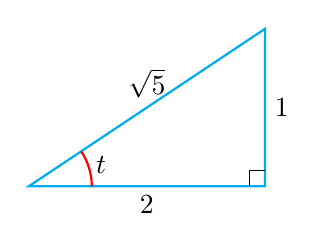
\begin{tikzpicture}[=>stealth]
\draw[thick,cyan](0,0)--(3,0)--(3,2)--cycle;
\draw(3,1)node[right]{1}
(1.5,0)node[below]{2}
(1.5,1)node[above]{$\sqrt{5}$};
\draw(2.8,0)--(2.8,0.2)--(3,0.2);
\coordinate (a) at (0.5,0);
\coordinate (b) at (0,0);
\coordinate (c) at (0.5,0.33);
\draw
pic[thick, draw = red, angle radius = 0.8cm, "$t$" , angle eccentricity = 1.2]{angle=a--b--c};
\end{tikzpicture}
\end{figure}

$\implies\hspace{0.5cm} \sin t = \dfrac{1}{\sqrt{5}}\hspace{0.4cm}$ and $\hspace{0.4cm} \cos t = \dfrac{2}{\sqrt{5}}$


Hence, at $\hspace{0.3cm} t = \arctan\dfrac{1}{2}$

$$x' = \frac{-3}{\sqrt{5}}\hspace{0.2cm} , \hspace{0.2cm} y' = \frac{4}{\sqrt{5}}\hspace{0.2cm} , \hspace{0.2cm} x'' = \frac{-6}{\sqrt{5}}\hspace{0.2cm} \text{and} \hspace{0.2cm} y'' = \frac{-2}{\sqrt{5}}$$

Therefore, the radius of curvature
\begin{align*}
\rho & = \frac{\Big[\big[x'(t)\big]^2 + \big[y'(t)\big]^2\Big]^{\dfrac{3}{2}}}{x'(t)y''(t) - y'(t)x''(t)}
 = \frac{\Big(\dfrac{9}{5} + \dfrac{16}{5}\Big)}{\Big(\dfrac{6}{5} + \dfrac{24}{5}\Big)}
 = \frac{5\sqrt{5}}{6}\\
\end{align*}

The curvature $\hspace{0.2cm} K = \dfrac{6}{5\sqrt{5}}$.
\end{solution}


\subsection{The Circle of Curvature}
The circle of curvature of a curve at a point $P$ on it is the circle of radius $P($ radius of curvature$)$ lying on the concave side of the circle and tangent to it.

% DIAGRAM 33

\begin{figure}[H]
\centering
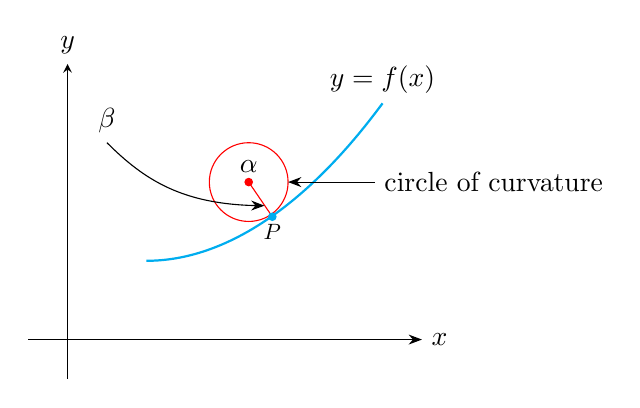
\begin{tikzpicture}[=>stealth]
\draw[-Stealth](-0.5,0)--(4.5,0)node[right]{$x$};
\draw[-stealth](0,-0.5)--(0,3.5)node[above]{$y$};
\draw[thick,cyan](1,1)parabola[bend at start](4,3)node[above,black]{$y = f(x)$};
\draw[red](2.3,2)circle[radius=0.5cm];
\draw[red](2.3,2)--(2.6,1.56);
\draw(2.6,1.56)node[scale=0.8,below]{$P$}
(2.3,2)node[shape=circle,fill=red,draw=red,scale=0.01cm]{}
(2.6,1.56)node[shape=circle,fill=cyan,draw=cyan,scale=0.01cm]{}
(2.3,2)node[above]{$\alpha$}
(3.9,2)node[right]{circle of curvature}
(0.5,2.5)node[above]{$\beta$};
\draw[-Stealth](3.9,2)--(2.8,2);
\draw[-Stealth](0.5,2.5)..controls(1,2)and(1.5,1.7)..(2.5,1.7);
\end{tikzpicture}
\end{figure}

The centre of curvature for a point $P(x,y)$ of a curve is the centre $C$ of the circle of curvature at $P$. The coordinates $(\alpha , \beta)$ of the centre of curvature are given by 
$$\alpha =  x - \frac{\dfrac{dy}{dx}\Big[1 +\Big(\dfrac{dy}{dx}\Big)^2\Big] }{\Big(\dfrac{d^2y}{dx^2}\Big)}\hspace{1cm}\text{and} \hspace{1cm} \beta = y+ \frac{1 + \Big(\dfrac{dy}{dx}\Big)^2}{\Big(\dfrac{d^2y}{dx^2}\Big)}$$


\begin{exa}


Find the equation of the circle of curvature of he curve $\hspace{0.3cm} 2xy + x + y = 4$ at the point $P(1,1)$.
\end{exa}


\begin{solution}
$$(x - \alpha)^2 + (y - \beta)^2 = \rho^2$$
Differentiating we have $\hspace{0.3cm}2y + 2xy' + 1 + y' = 0$


At $P(1,1)\hspace{0.2cm} , \hspace{0.4cm} y' = -1\hspace{0.2cm}$ and $\hspace{0.2cm} (1 + y')^2 = 2$


Differentiating again, we obtain $\hspace{0.4cm} 2y' + 2y' + 2xy'' + y'' =0$


$\implies\hspace{0.4cm} 4y' + (2x + 1)y'' = 0\hspace{0.2cm}$ At $(1,1)\hspace{0.4cm} y'' = \dfrac{4}{3}$


Thus $\hspace{0.3cm} K = \dfrac{2}{3\sqrt{2}} \hspace{0.3cm} \implies \hspace{0.3cm} \rho = \dfrac{3\sqrt{2}}{2}$


$$\text{And}\hspace{0.5cm} \alpha = x - \frac{y' (1 + y'^2)}{y''}= \frac{5}{2}$$

$$\beta = y + \frac{1 + y'^2}{y''} = \frac{5}{2}$$

$\implies\hspace{0.5cm} $ the centre of curvature is $\Big(\dfrac{5}{2},\dfrac{5}{2}\Big)$.


Therefore, the equation of the circle of curvature $$ \Big( x - \frac{5}{2}\Big)^2 + \Big(y - \frac{5}{2}\Big)^2 = \frac{9}{2}$$
\end{solution}


\subsection{Intrinsic Coordinates}

% DIAGRAM 34

\begin{figure}[H]
\centering
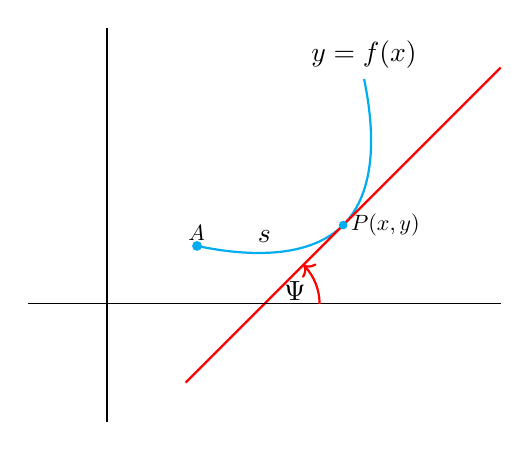
\begin{tikzpicture}
%\draw[-Stealth](-2,0)--(2,0);
%\draw(0,-0.5)--(0,2);
\draw[thick,cyan,rotate=45](0,0)parabola(1.5,1.125)node[black,above]{$y=f(x)$};
\draw[thick,cyan,rotate=45](0,0)parabola(-1.5,1.125)node[shape=circle,fill=cyan,draw=cyan,scale=0.01cm]{};
\draw[red,thick](-2,-2)--(2,2);
\draw(0,0)node[shape=circle,fill=cyan,draw=cyan,scale=0.01cm]{}
(0,0)node[right,scale=0.8]{$P(x,y)$}
(-1.86,-0.3)node[above,scale=0.8]{$A$}
(-1,-0.35)node[above]{$s$};
\draw(-4,-1)--(2,-1)
(-3,-2.5)--(-3,2.5);
\coordinate (a) at (0,-1);
\coordinate (b) at (-1,-1);
\coordinate (c) at (-0.5,-0.5);
\draw
pic[thick ,angle radius  = 0.7cm, draw=red,->,"$\Psi$"]{angle=a--b--c};
\end{tikzpicture}
\end{figure}

$s = $ Length of the curve from  $A$ to $P$


$\Psi = $ the angle which the tangent to the curve at $P$ makes with the positive $x -$ axis.


$s$ and $\Psi$ are called intrinsic coordinates of $P$ and the point is written $(s,\Psi)$.


From elementary calculus
$\hspace{0.3cm}\dfrac{dy}{dx} = \tan \Psi$. Thus

$$\frac{d^2y}{dx^2} = \frac{d(\tan \Psi)}{dx} = \sec^2\Psi \dfrac{d\Psi}{dx}$$

$$\frac{d\Psi}{dx}= \frac{\dfrac{d^2y}{dx^2}}{\sec^2\Psi}$$

$$\implies \hspace{0.5cm} \frac{dx}{d\Psi} = \frac{\sec^2 \Psi}{d^2y/dx^2}$$


But $\hspace{0.3cm}\displaystyle{\frac{dy}{dx} = \tan \Psi = \frac{\sin \Psi}{\cos \Psi}}\hspace{0.4cm}$
Also $\hspace{0.4cm}\displaystyle{\frac{dy}{dx} = \frac{dy/ds}{dx/ds} =\frac{\sin \Psi}{\cos \Psi}}$


$$\implies\hspace{0.4cm} \frac{dy}{ds} = \sin \Psi \hspace{0.5cm}\text{and}\hspace{0.5cm} \frac{dx}{ds} = \cos \Psi$$


\begin{exa}


Write the equation $y = \cosh x$ in intrinsic coordinates.

$$\dfrac{dy}{dx} = \sinh\hspace{0.4cm} , \hspace{0.4cm} \frac{ds}{dx} = \sqrt{1 + \Big(\dfrac{dy}{dx}\Big)^2}$$

So that $\hspace{0.3cm}\displaystyle{\frac{ds}{dx} = \sqrt{1 + \sinh^x}=\sqrt{\cosh^2x}=\cosh x}$

\begin{align*}
\frac{ds}{dx} =\cosh x \implies s & = \int \frac{ds}{dx}\hspace{0.1cm}dx \\
& = \int \cosh x\hspace{0.1cm}dx
\end{align*}

$$\implies\hspace{0.5cm} s(x) = \sinh x + c$$

Particularly, if $s = 0$ at $x = 0$, we get $c = 0$ so that $s(x) = \sinh x$

$$s = \sinh x \implies x = \sinh^{-1}s$$


But $\hspace{0.5cm} y = \cosh x = \sqrt{1 + \sinh^2x} = \sqrt{1 + s^2}$


$\therefore\hspace{0.4cm} y = \sqrt{1 + s^2}$


But $\hspace{0.5cm} \tan \Psi = \dfrac{dy}{dx} = \sinh x$


$\implies\hspace{0.5cm} \tan \Psi  = s$


$\implies\hspace{0.5cm} \Psi  = \tan^{-1}s$


Curvature in intrinsic coordinates $\hspace{0.4cm}\displaystyle{ K = \frac{d\Psi}{ds} = \frac{1}{1 + s^2}}$


In Cartesian coordinates $\hspace{0.4cm}\displaystyle{ K = \frac{1}{1 + \sinh^2x} = \frac{1}{\cosh^x}}$


Compare:
\begin{align*}
K & = \frac{y''}{\Big(1 + (y')^2\Big)^{\dfrac{3}{2}}} = \frac{\cosh x}{\Big(1 + \sinh^2x\Big)^{\dfrac{3}{2}}}\\\\
& = \frac{\cosh x}{\Big(\cosh^2x\Big)^{\dfrac{3}{2}}}\\
& = \frac{1}{\cosh^2x}
\end{align*}

\pagebreak
\end{exa}

\subsection{Practice Problems}

These are the tutorial questions for this section, worked in full.

\begin{problem}
Let $\lim\limits_{x\rightarrow c}f(x) = L$. Given $c$, $L$ and $\varepsilon>0$,
determine $\delta>0$ so that $\left|f(x)-L\right|<\varepsilon$ whenever
$0<\left|x-c\right|<\delta$.
\begin{enumerate}
\item[(a)] $f(x) = 2x-3$, $c=2$, $L=1$, $\varepsilon = 0.001$
\item[(b)] $f(x) = \dfrac{x^2-9}{x+3}$, $c=-3$, $L=-6$, $\varepsilon = 0.005$
\item[(c)] $f(x) = \dfrac{1}{x}$, $c=2$, $L=\dfrac12$, $\varepsilon = 0.002$
\item[(d)] $f(x) = \dfrac{4}{x+3}$, $c=1$, $L=1$, $\varepsilon = 0.001$
\end{enumerate}
\end{problem}
\begin{solution}
In each case the method is the same: express $\left|f(x)-L\right|$ in terms of
$\left|x-c\right|$ and make the result smaller than $\varepsilon$.

\subhead{(a)}
$$\left|2x-3-1\right| = \left|2x-4\right| = 2\left|x-2\right| < 0.001
\implies \left|x-2\right| < 0.0005 .$$
So $\delta = 0.0005$ works.

\subhead{(b)}
For $x\neq -3$, $\dfrac{x^2-9}{x+3} = x-3$, so
$$\left|(x-3)-(-6)\right| = \left|x+3\right| < 0.005 ,$$
and $\delta = 0.005$ works. The removable discontinuity at $x=-3$ is irrelevant,
since the definition never uses the value at $x=c$.

\subhead{(c)}
$$\left|\frac{1}{x} - \frac{1}{2}\right| = \frac{\left|2-x\right|}{2\left|x\right|}.$$
The factor $\dfrac{1}{\left|x\right|}$ must be controlled first. Restricting
$\left|x-2\right|<1$ gives $1<x<3$, hence $2\left|x\right|>2$ and
$$\left|\frac{1}{x}-\frac{1}{2}\right| < \frac{\left|x-2\right|}{2} .$$
Requiring this to be below $0.002$ gives $\left|x-2\right|<0.004$, so
$\delta = \min\{1, 0.004\} = 0.004$.

\subhead{(d)}
$$\left|\frac{4}{x+3} - 1\right| = \frac{\left|4 - (x+3)\right|}{\left|x+3\right|}
= \frac{\left|1-x\right|}{\left|x+3\right|}.$$
Restricting $\left|x-1\right|<1$ gives $0<x<2$, so $\left|x+3\right|>3$ and the
quotient is less than $\dfrac{\left|x-1\right|}{3}$. Requiring this below
$0.001$ gives $\left|x-1\right|<0.003$, so $\delta = \min\{1,0.003\} = 0.003$.
\end{solution}

\begin{problem}
Show $\lim\limits_{x\rightarrow c}f(x) = L$ directly from the definition, by
finding a $\delta>0$ for every $\varepsilon>0$.
\begin{enumerate}
\item[(a)] $f(x) = 3x-5$, $c=1$, $L=-2$
\item[(b)] $f(x) = \dfrac{x^2-4}{x-2}$, $c=2$, $L=4$
\item[(c)] $f(x) = \dfrac{1}{x+3}$, $c=-2$, $L=1$
\item[(d)] $f(x) = \dfrac{x-1}{x+1}$, $c=0$, $L=-1$
\end{enumerate}
\end{problem}
\begin{solution}
\subhead{(a)}
$\left|3x-5+2\right| = 3\left|x-1\right| < \varepsilon$ exactly when
$\left|x-1\right| < \dfrac{\varepsilon}{3}$, so take
$\delta = \dfrac{\varepsilon}{3}$.

\subhead{(b)}
For $x\neq 2$, $\dfrac{x^2-4}{x-2} = x+2$, so
$\left|(x+2)-4\right| = \left|x-2\right| < \varepsilon$ and
$\delta = \varepsilon$ works.

\subhead{(c)}
$$\left|\frac{1}{x+3} - 1\right| = \frac{\left|1-(x+3)\right|}{\left|x+3\right|}
= \frac{\left|x+2\right|}{\left|x+3\right|}.$$
Restricting $\left|x+2\right| < \dfrac12$ gives $\left|x+3\right| > \dfrac12$,
so the quotient is below $2\left|x+2\right|$. Take
$\delta = \min\Big\{\dfrac12, \dfrac{\varepsilon}{2}\Big\}$.

\subhead{(d)}
$$\left|\frac{x-1}{x+1} + 1\right| = \left|\frac{x-1+x+1}{x+1}\right|
= \frac{2\left|x\right|}{\left|x+1\right|}.$$
Restricting $\left|x\right| < \dfrac12$ gives $\left|x+1\right| > \dfrac12$, so
the quotient is below $4\left|x\right|$. Take
$\delta = \min\Big\{\dfrac12, \dfrac{\varepsilon}{4}\Big\}$.
\end{solution}

\begin{note}
Part (b) of the previous question is printed in some copies as
$f(x) = \dfrac{x^2-4}{x+2}$. That function tends to $0$ as $x\rightarrow 2$, not
to $4$; the denominator must be $x-2$ for the stated limit to hold.
\end{note}

\begin{problem}
Evaluate the limits.
$$(a)\hspace{0.2cm}\lim_{h\rightarrow 0}\frac{\sqrt{x+h}-\sqrt{x}}{h}\ (x>0)
\hspace{0.6cm}(b)\hspace{0.2cm}\lim_{x\rightarrow 2}\frac{x^3-8}{x-2}
\hspace{0.6cm}(c)\hspace{0.2cm}\lim_{x\rightarrow 2}\frac{4-x^2}{3-\sqrt{x^2+5}}
\hspace{0.6cm}(d)\hspace{0.2cm}\lim_{x\rightarrow 1^+}\frac{x}{1-x}$$
$$(e)\hspace{0.2cm}\lim_{x\rightarrow 2}\sqrt{\frac{2x+5}{3x-2}}
\hspace{0.6cm}(f)\hspace{0.2cm}\lim_{x\rightarrow\infty}\frac{2x^2+7x+5}{x^3+2x+1}
\hspace{0.6cm}(g)\hspace{0.2cm}\lim_{x\rightarrow-\infty}\frac{x^2+4}{x+2}
\hspace{0.6cm}(h)\hspace{0.2cm}\lim_{x\rightarrow 0^-}\frac{1+x}{x}$$
\end{problem}
\begin{solution}
\subhead{(a)}
Rationalise the numerator:
$$\frac{\sqrt{x+h}-\sqrt{x}}{h}\cdot\frac{\sqrt{x+h}+\sqrt{x}}{\sqrt{x+h}+\sqrt{x}}
= \frac{h}{h\big(\sqrt{x+h}+\sqrt{x}\big)}
= \frac{1}{\sqrt{x+h}+\sqrt{x}}\longrightarrow \frac{1}{2\sqrt{x}} .$$

\subhead{(b)}
Factor: $x^3-8 = (x-2)(x^2+2x+4)$, so the quotient is $x^2+2x+4\rightarrow 12$.

\subhead{(c)}
Both parts vanish at $x=2$. Rationalise the denominator:
$$\frac{4-x^2}{3-\sqrt{x^2+5}}\cdot\frac{3+\sqrt{x^2+5}}{3+\sqrt{x^2+5}}
= \frac{\big(4-x^2\big)\big(3+\sqrt{x^2+5}\big)}{9-\big(x^2+5\big)}
= \frac{\big(4-x^2\big)\big(3+\sqrt{x^2+5}\big)}{4-x^2}.$$
Cancelling gives $3+\sqrt{x^2+5}\rightarrow 3+3 = 6$.

\subhead{(d)}
As $x\rightarrow 1^+$ the numerator tends to $1$ while $1-x\rightarrow 0$
through \emph{negative} values, so the quotient tends to $-\infty$.

\subhead{(e)}
The function is continuous at $x=2$, so substitute:
$\sqrt{\dfrac{9}{4}} = \dfrac{3}{2}$.

\subhead{(f)}
Divide numerator and denominator by $x^3$:
$$\frac{\frac{2}{x} + \frac{7}{x^2} + \frac{5}{x^3}}{1 + \frac{2}{x^2} + \frac{1}{x^3}}
\longrightarrow \frac{0}{1} = 0 .$$
The denominator has the higher degree, so the limit is $0$.

\subhead{(g)}
Here the numerator has the higher degree. Dividing by $x$,
$$\frac{x + \frac{4}{x}}{1 + \frac{2}{x}} \longrightarrow -\infty
\quad\text{as } x\rightarrow -\infty .$$

\subhead{(h)}
As $x\rightarrow 0^-$ the numerator tends to $1$ and $x\rightarrow 0$ through
negative values, so the quotient tends to $-\infty$.
\end{solution}

\begin{problem}
For the given $f$, find
$\displaystyle{\lim_{h\rightarrow 0}\frac{f(x+h)-f(x)}{h}}$.
$$(a)\hspace{0.4cm} f(x) = x^2-3x \hspace{2cm} (b)\hspace{0.4cm} f(x) = \sqrt{5x+1}$$
\end{problem}
\begin{solution}
This is the derivative computed from first principles.

\subhead{(a)}
$$\frac{\big[(x+h)^2 - 3(x+h)\big] - \big[x^2-3x\big]}{h}
= \frac{2xh + h^2 - 3h}{h} = 2x + h - 3 \longrightarrow 2x-3 .$$

\subhead{(b)}
Rationalising the numerator,
$$\frac{\sqrt{5x+5h+1}-\sqrt{5x+1}}{h}
= \frac{5h}{h\big(\sqrt{5x+5h+1}+\sqrt{5x+1}\big)}
\longrightarrow \frac{5}{2\sqrt{5x+1}} .$$
\end{solution}

\begin{problem}
Evaluate the limits.
$$(a)\hspace{0.2cm}\lim_{x\rightarrow 2}\frac{x^2+x-6}{x^2-6}
\hspace{0.8cm}(b)\hspace{0.2cm}\lim_{x\rightarrow 0}\frac{x-\sin 2x}{x+\sin 2x}
\hspace{0.8cm}(c)\hspace{0.2cm}\lim_{x\rightarrow\frac{\pi}{4}}(1-\tan x)\sec 2x
\hspace{0.8cm}(d)\hspace{0.2cm}\lim_{x\rightarrow 1^+}x^{\frac{1}{x-1}}$$
$$(e)\hspace{0.3cm}\lim_{x\rightarrow 0^+}\big(x^2\ln x\big)
\hspace{1cm}(f)\hspace{0.3cm}\lim_{x\rightarrow 0}\big(\csc x - \cot x\big)
\hspace{1cm}(g)\hspace{0.3cm}\lim_{x\rightarrow\frac{\pi}{2}}(\tan x)^{\cos x}$$
\end{problem}
\begin{solution}
\subhead{(a)}
Not indeterminate: substituting gives $\dfrac{4+2-6}{4-6} = \dfrac{0}{-2} = 0$.
A zero numerator with a non-zero denominator is simply zero.

\subhead{(b)}
Of the form $\dfrac{0}{0}$. Dividing above and below by $x$,
$$\frac{1 - \frac{\sin 2x}{x}}{1 + \frac{\sin 2x}{x}}
\longrightarrow \frac{1-2}{1+2} = -\frac{1}{3},$$
using $\dfrac{\sin 2x}{x}\rightarrow 2$.

\subhead{(c)}
Of the form $0\cdot\infty$. Write it as a quotient:
$$\frac{1-\tan x}{\cos 2x} \qquad\Big(\tfrac00\Big),$$
and apply l'H\^{o}pital:
$$\frac{-\sec^2x}{-2\sin 2x} = \frac{\sec^2 x}{2\sin 2x}
\longrightarrow \frac{2}{2} = 1 .$$

\subhead{(d)}
Of the form $1^{\infty}$. Taking logarithms, with $y = x^{1/(x-1)}$,
$$\ln y = \frac{\ln x}{x-1} \qquad\Big(\tfrac00\Big)
\longrightarrow \frac{1/x}{1} = 1 ,$$
so $y\rightarrow e$.

\subhead{(e)}
Of the form $0\cdot(-\infty)$. Write $x^2\ln x = \dfrac{\ln x}{x^{-2}}$, of type
$\dfrac{-\infty}{\infty}$, and apply l'H\^{o}pital:
$$\frac{1/x}{-2x^{-3}} = -\frac{x^2}{2}\longrightarrow 0 .$$

\subhead{(f)}
Of the form $\infty-\infty$. Combine over a common denominator:
$$\csc x - \cot x = \frac{1-\cos x}{\sin x} \qquad\Big(\tfrac00\Big)
\longrightarrow \frac{\sin x}{\cos x} = \tan x \longrightarrow 0 .$$

\subhead{(g)}
Of the form $\infty^0$. With $y = (\tan x)^{\cos x}$,
$$\ln y = \cos x\ln\tan x = \frac{\ln\tan x}{\sec x}
\qquad\Big(\tfrac{\infty}{\infty}\Big).$$
Differentiating,
$$\frac{\sec^2x/\tan x}{\sec x\tan x}
= \frac{\sec x}{\tan^2 x} = \frac{\cos x}{\sin^2 x}\longrightarrow 0 ,$$
so $y\rightarrow e^0 = 1$.
\end{solution}

\begin{problem}
Sketch each function, find its discontinuities, say why continuity fails there,
and state which discontinuities are removable.
$$(a)\ f(x) = \frac{\left|x\right|}{x}\hspace{1cm}
(b)\ f(x) = \frac{x^2-3x-10}{x+2}\hspace{1cm}
(c)\ f(x) = \frac{x^4-1}{x^2-1}$$
$$(d)\ f(x) = \begin{cases} x+3 & x\geq 2\\ x^2+1 & x<2\end{cases}
\hspace{1cm}
(e)\ f(x) = \begin{cases} 4-x, & x\geq 3\\ x-2, & 0<x<3\\ x-1, & x\leq 0\end{cases}$$
\end{problem}
\begin{solution}
\subhead{(a)}
$f(x) = 1$ for $x>0$ and $-1$ for $x<0$, undefined at $x=0$. The one-sided
limits are $1$ and $-1$, so no limit exists at $0$: a \emph{jump}
discontinuity, and \textbf{not} removable.

\subhead{(b)}
$\dfrac{x^2-3x-10}{x+2} = \dfrac{(x-5)(x+2)}{x+2} = x-5$ for $x\neq -2$. The
limit at $-2$ is $-7$ but the function is undefined there: a \emph{removable}
discontinuity, repaired by setting $f(-2) = -7$.

\subhead{(c)}
$\dfrac{x^4-1}{x^2-1} = \dfrac{(x^2-1)(x^2+1)}{x^2-1} = x^2+1$ for
$x\neq\pm 1$. Both $x=1$ and $x=-1$ are \emph{removable}, repaired by setting
$f(\pm 1) = 2$.

\subhead{(d)}
The pieces meet at $x=2$. From the left $x^2+1\rightarrow 5$; from the right
$x+3\rightarrow 5$; and $f(2) = 5$. The limits agree with the value, so $f$ is
in fact \emph{continuous} at $2$ and has no discontinuity at all.

\subhead{(e)}
Two junctions. At $x=0$: from the left $x-1\rightarrow -1$, which is $f(0)$;
from the right $x-2\rightarrow -2$. The one-sided limits differ, so there is a
\emph{jump}, not removable. At $x=3$: from the left $x-2\rightarrow 1$; from the
right $4-x\rightarrow 1$, and $f(3) = 1$. Continuous there.
\end{solution}

\begin{problem}
Find the values $x_0$ prescribed by Rolle's theorem.
\begin{enumerate}
\item[(a)] $f(x) = x^3-12x$ on $0\leq x\leq 2\sqrt3$
\item[(b)] $f(x) = \sin x$ on $0\leq x\leq\pi$
\item[(c)] $f(x) = \cos x$ on $\dfrac{\pi}{2}\leq x\leq\dfrac{3\pi}{2}$
\end{enumerate}
\end{problem}
\begin{solution}
Rolle's theorem requires $f$ continuous on $[a,b]$, differentiable on $(a,b)$
and $f(a) = f(b)$; it then supplies $x_0\in(a,b)$ with $f'(x_0) = 0$.

\subhead{(a)}
$f(0) = 0$ and $f(2\sqrt3) = 24\sqrt3 - 24\sqrt3 = 0$, so the hypotheses hold.
$$f'(x) = 3x^2-12 = 0 \implies x = \pm 2 ,$$
and only $x_0 = 2$ lies in $\big(0, 2\sqrt3\big)$.

\subhead{(b)}
$\sin 0 = \sin\pi = 0$ and $f'(x) = \cos x = 0$ gives
$x_0 = \dfrac{\pi}{2}$, which lies in $(0,\pi)$.

\subhead{(c)}
$\cos\dfrac{\pi}{2} = \cos\dfrac{3\pi}{2} = 0$ and $f'(x) = -\sin x = 0$ gives
$x = 0$ or $\pi$; only $x_0 = \pi$ lies in the interval.
\end{solution}

\begin{problem}
Does Rolle's theorem apply to
$$(a)\hspace{0.3cm} f(x) = \frac{x^2-4x}{x-2}
\hspace{2cm}(b)\hspace{0.3cm} f(x) = \frac{x^2-4x}{x+2}\ ?$$
\end{problem}
\begin{solution}
Both vanish at $x=0$ and $x=4$, so $[0,4]$ is the natural interval to test.

\subhead{(a)}
No. The function is undefined at $x=2$, which lies inside $(0,4)$, so it is
neither continuous on $[0,4]$ nor differentiable on $(0,4)$. The hypotheses fail
and the conclusion need not hold.

\subhead{(b)}
Yes. The only singularity is at $x=-2$, outside $[0,4]$, so $f$ is continuous
and differentiable throughout and $f(0) = f(4) = 0$. Differentiating,
$$f'(x) = \frac{(2x-4)(x+2) - \big(x^2-4x\big)}{(x+2)^2}
= \frac{x^2+4x-8}{(x+2)^2},$$
which vanishes when $x^2+4x-8 = 0$, that is $x = -2\pm 2\sqrt3$. The root
$x_0 = -2+2\sqrt3 \approx 1.46$ lies in $(0,4)$, as Rolle guarantees.
\end{solution}

\begin{problem}
Find the value $x_0$ prescribed by the Mean Value theorem.
\begin{enumerate}
\item[(a)] $f(x) = 3x^2+4x-3$, $a=1$, $b=3$
\item[(b)] $f(x) = x^3$, $0\leq x\leq 6$
\item[(c)] $f(x) = \ln x$, $1\leq x\leq 2e$
\end{enumerate}
\end{problem}
\begin{solution}
The theorem gives $x_0\in(a,b)$ with
$f'(x_0) = \dfrac{f(b)-f(a)}{b-a}$.

\subhead{(a)}
$f(3) = 36$, $f(1) = 4$, so the slope is $\dfrac{36-4}{2} = 16$. Then
$f'(x) = 6x+4 = 16$ gives $x_0 = 2$.

\subhead{(b)}
The slope is $\dfrac{216-0}{6} = 36$, and $f'(x) = 3x^2 = 36$ gives
$x = \pm 2\sqrt3$; only $x_0 = 2\sqrt3 \approx 3.46$ lies in $(0,6)$.

\subhead{(c)}
The slope is $\dfrac{\ln 2e - \ln 1}{2e-1} = \dfrac{1+\ln 2}{2e-1}$, and
$f'(x) = \dfrac1x$ gives
$$x_0 = \frac{2e-1}{1+\ln 2} \approx 2.62 ,$$
which lies in $(1, 2e)$.
\end{solution}

\begin{problem}
Use the Mean Value theorem to approximate
$$(a)\ \sqrt{15}\hspace{1cm} (b)\ \sqrt[6]{65}\hspace{1cm}
(c)\ (3.001)^3\hspace{1cm} (d)\ \frac{1}{999}$$
\end{problem}
\begin{solution}
The theorem gives $f(b) - f(a) = f'(c)(b-a)$ for some $c$ between $a$ and $b$.
Choosing $a$ where $f$ is known exactly and $b$ the target, and approximating
$f'(c)$ by its value at the known endpoint, gives the estimates below.

\subhead{(a)}
Take $f(x) = \sqrt x$ on $[15,16]$. Then
$4 - \sqrt{15} = \dfrac{1}{2\sqrt c}$ with $15<c<16$, so
$$\sqrt{15} \approx 4 - \frac{1}{2\sqrt{16}} = 4 - \frac18 = 3.875 ,$$
against the true value $3.8730$.

\subhead{(b)}
Take $f(x) = x^{1/6}$ on $[64,65]$, so $f'(x) = \dfrac{1}{6}x^{-5/6}$ and
$$\sqrt[6]{65} \approx 2 + \frac{1}{6\cdot 32} = 2 + \frac{1}{192}
\approx 2.00521 ,$$
against $2.00517$.

\subhead{(c)}
Take $f(x) = x^3$ on $[3, 3.001]$, so $f'(x) = 3x^2$ and
$$(3.001)^3 \approx 27 + 3(9)(0.001) = 27.027 ,$$
against $27.027009$.

\subhead{(d)}
Take $f(x) = \dfrac1x$ on $[999,1000]$, so $f'(x) = -\dfrac{1}{x^2}$ and
$$\frac{1}{999} \approx \frac{1}{1000} + \frac{1}{1000^2} = 0.001001 ,$$
against $0.001001001\ldots$
\end{solution}

\begin{problem}
Use the Mean Value theorem to prove that
$\tan x > x$ for $0 < x < \dfrac{\pi}{2}$.
\end{problem}
\begin{solution}
Fix $x$ with $0<x<\dfrac{\pi}{2}$ and apply the theorem to $f(t) = \tan t$ on
$[0,x]$, where it is continuous and differentiable. There is $c\in(0,x)$ with
$$\frac{\tan x - \tan 0}{x - 0} = \sec^2 c ,
\qquad\text{that is}\qquad \tan x = x\sec^2 c .$$
Since $0<c<\dfrac{\pi}{2}$ we have $0<\cos c<1$, hence $\sec^2 c>1$, and as
$x>0$,
$$\tan x = x\sec^2c > x .$$
\end{solution}

\begin{problem}
Find $x_0$ as prescribed by the generalized Mean Value theorem for
$f(x) = 3x+2$ and $g(x) = x^2+1$ on $1\leq x\leq 4$.
\end{problem}
\begin{solution}
Cauchy's form states that
$$\frac{f(b)-f(a)}{g(b)-g(a)} = \frac{f'(x_0)}{g'(x_0)}$$
for some $x_0\in(a,b)$, provided $g'$ does not vanish there. Here
$$\frac{f(4)-f(1)}{g(4)-g(1)} = \frac{14-5}{17-2} = \frac{9}{15} = \frac{3}{5},$$
while $\dfrac{f'(x)}{g'(x)} = \dfrac{3}{2x}$. Setting these equal,
$$\frac{3}{2x_0} = \frac{3}{5} \implies x_0 = \frac{5}{2},$$
which lies in $(1,4)$. Note $g'(x) = 2x\neq 0$ throughout, as required.
\end{solution}


\begin{problem}
Examine each geometric series for convergence, and find the sum where it
converges.
$$(a)\ 1+\frac12+\frac14+\frac18+\cdots\hspace{1cm}
(b)\ 4-1+\frac14-\frac{1}{16}+\cdots\hspace{1cm}
(c)\ 1+\frac32+\frac94+\frac{27}{8}+\cdots$$
\end{problem}
\begin{solution}
A geometric series $\sum ar^{n-1}$ converges precisely when
$\left|r\right|<1$, to $\dfrac{a}{1-r}$.

\subhead{(a)}
$a = 1$, $r = \dfrac12$. Since $\left|r\right|<1$ it converges to
$\dfrac{1}{1-\frac12} = 2$.

\subhead{(b)}
$a = 4$, $r = -\dfrac14$. Since $\left|r\right|<1$ it converges to
$\dfrac{4}{1+\frac14} = \dfrac{4}{\frac54} = \dfrac{16}{5}$.

\subhead{(c)}
$a = 1$, $r = \dfrac32 > 1$, so the series diverges.
\end{solution}

\begin{problem}
Find the sum of each series.
$$(a)\ \sum_{n=1}^{\infty}3^{-n}\hspace{0.7cm}
(b)\ \sum_{n=1}^{\infty}\frac{1}{(2n-1)(2n+1)}\hspace{0.7cm}
(c)\ \sum_{n=1}^{\infty}\frac{1}{n(n+2)}\hspace{0.7cm}
(d)\ \sum_{n=1}^{\infty}\frac{1}{n(n+1)(n+2)}$$
\end{problem}
\begin{solution}
\subhead{(a)}
Geometric with $a = \dfrac13$, $r = \dfrac13$, so the sum is
$\dfrac{1/3}{1-1/3} = \dfrac12$.

\subhead{(b)}
Partial fractions give
$\dfrac{1}{(2n-1)(2n+1)} = \dfrac12\Big(\dfrac{1}{2n-1} - \dfrac{1}{2n+1}\Big)$,
so the partial sum telescopes:
$$S_N = \frac12\Big(1 - \frac{1}{2N+1}\Big)\longrightarrow \frac12 .$$

\subhead{(c)}
Here $\dfrac{1}{n(n+2)} = \dfrac12\Big(\dfrac1n - \dfrac{1}{n+2}\Big)$, and the
terms cancel in pairs two apart, leaving the first two:
$$S_N = \frac12\Big(1 + \frac12 - \frac{1}{N+1} - \frac{1}{N+2}\Big)
\longrightarrow \frac12\cdot\frac32 = \frac34 .$$

\subhead{(d)}
Here
$$\frac{1}{n(n+1)(n+2)}
= \frac{1}{2n} - \frac{1}{n+1} + \frac{1}{2(n+2)} ,$$
and telescoping leaves
$$S_N \longrightarrow \frac12 - \frac12 + \frac14 = \frac14 .$$
\end{solution}

\begin{problem}
Verify that the integral test applies, and use it to determine convergence.
$$(a)\ \sum\frac1n\hspace{1cm}(b)\ \sum\frac{50}{n(n+1)}\hspace{1cm}
(c)\ \sum\frac{n}{n^2+1}\hspace{1cm}(d)\ \sum\frac{1}{(2n+1)^2}$$
\end{problem}
\begin{solution}
In each case the associated function is positive, continuous and eventually
decreasing on $[1,\infty)$, so the test applies and the series converges exactly
when the integral does.

\subhead{(a)}
$\displaystyle{\int_1^{\infty}\frac{dx}{x} = \lim_{b\rightarrow\infty}\ln b
= \infty}$, so the harmonic series \emph{diverges}.

\subhead{(b)}
$\dfrac{50}{x(x+1)} = 50\Big(\dfrac1x - \dfrac{1}{x+1}\Big)$, so
$$\int_1^{\infty}\frac{50\,dx}{x(x+1)}
= 50\Big[\ln\frac{x}{x+1}\Big]_1^{\infty} = 50\big(0 - \ln\tfrac12\big)
= 50\ln 2 ,$$
finite, so the series \emph{converges}.

\subhead{(c)}
$$\int_1^{\infty}\frac{x\,dx}{x^2+1}
= \Big[\tfrac12\ln\big(x^2+1\big)\Big]_1^{\infty} = \infty ,$$
so the series \emph{diverges}. Note the terms tend to $0$, which by itself
proves nothing.

\subhead{(d)}
$$\int_1^{\infty}\frac{dx}{(2x+1)^2}
= \Big[-\frac{1}{2(2x+1)}\Big]_1^{\infty} = \frac16 ,$$
finite, so the series \emph{converges}.
\end{solution}

\begin{problem}
Determine convergence by comparison.
$$(a)\ \sum\frac{1}{n^3-1}\hspace{1cm}(b)\ \sum\frac{1}{\sqrt[3]{n}}
\hspace{1cm}(c)\ \sum\frac{1}{n^{n-1}}\hspace{1cm}(d)\ \sum\frac{n}{3n^2-4}$$
\end{problem}
\begin{solution}
\subhead{(a)}
For $n\geq 2$, $n^3 - 1 \geq \dfrac{n^3}{2}$, so
$\dfrac{1}{n^3-1}\leq\dfrac{2}{n^3}$. Since $\sum\dfrac{1}{n^3}$ is a
$p-$series with $p = 3 > 1$ it converges, so the given series
\emph{converges}.

\subhead{(b)}
$\dfrac{1}{\sqrt[3]{n}} = \dfrac{1}{n^{1/3}}$ is a $p-$series with
$p = \dfrac13 \leq 1$, so it \emph{diverges}.

\subhead{(c)}
For $n\geq 3$, $n^{n-1}\geq 2^{n-1}$, so
$\dfrac{1}{n^{n-1}}\leq\dfrac{1}{2^{n-1}}$, the terms of a convergent geometric
series. Hence it \emph{converges}.

\subhead{(d)}
For large $n$, $\dfrac{n}{3n^2-4}$ behaves like $\dfrac{1}{3n}$. Precisely, for
$n\geq 2$, $3n^2 - 4 \leq 3n^2$, so
$$\frac{n}{3n^2-4} \geq \frac{n}{3n^2} = \frac{1}{3n},$$
and $\sum\dfrac{1}{3n}$ diverges. Hence the series \emph{diverges}.
\end{solution}

\begin{problem}
Determine convergence by the ratio test.
$$(a)\ \sum\frac{(n+1)(n+2)}{n!}\hspace{1cm}(b)\ \sum\frac{5^n}{n!}
\hspace{1cm}(c)\ \sum\frac{n}{2^{2n}}\hspace{1cm}(d)\ \sum\frac{n^n}{n!}$$
\end{problem}
\begin{solution}
The test examines $L = \lim\left|\dfrac{a_{n+1}}{a_n}\right|$: convergence if
$L<1$, divergence if $L>1$, no conclusion if $L=1$.

\subhead{(a)}
$$\frac{a_{n+1}}{a_n} = \frac{(n+2)(n+3)}{(n+1)!}\cdot\frac{n!}{(n+1)(n+2)}
= \frac{n+3}{(n+1)^2}\longrightarrow 0 < 1 ,$$
so it \emph{converges}.

\subhead{(b)}
$$\frac{a_{n+1}}{a_n} = \frac{5^{n+1}}{(n+1)!}\cdot\frac{n!}{5^n}
= \frac{5}{n+1}\longrightarrow 0 < 1 ,$$
so it \emph{converges}.

\subhead{(c)}
$$\frac{a_{n+1}}{a_n} = \frac{n+1}{2^{2n+2}}\cdot\frac{2^{2n}}{n}
= \frac{1}{4}\cdot\frac{n+1}{n}\longrightarrow \frac14 < 1 ,$$
so it \emph{converges}.

\subhead{(d)}
$$\frac{a_{n+1}}{a_n} = \frac{(n+1)^{n+1}}{(n+1)!}\cdot\frac{n!}{n^n}
= \frac{(n+1)^n}{n^n} = \Big(1+\frac1n\Big)^n\longrightarrow e > 1 ,$$
so it \emph{diverges}.
\end{solution}

\begin{problem}
Show that the following alternating series converge.
$$(a)\ 1-\frac{1}{2^2}+\frac{1}{3^2}-\cdots\hspace{0.7cm}
(b)\ \frac12-\frac15+\frac{1}{10}-\frac{1}{17}+\cdots\hspace{0.7cm}
(c)\ \sum\frac{(-1)^{n-1}}{n!}\hspace{0.7cm}
(d)\ \sum\frac{(-1)^{n-1}}{2n-1}$$
\end{problem}
\begin{solution}
The alternating series test requires the absolute values to decrease
monotonically to $0$; both conditions are needed.

\subhead{(a)}
$a_n = \dfrac{1}{n^2}$ decreases and tends to $0$, so it converges. (It also
converges absolutely, being a $p-$series with $p=2$.)

\subhead{(b)}
The denominators are $n^2+1$, so $a_n = \dfrac{1}{n^2+1}$, which decreases to
$0$: it converges.

\subhead{(c)}
$a_n = \dfrac{1}{n!}$ decreases to $0$, so it converges. Its sum is
$1 - e^{-1}$.

\subhead{(d)}
$a_n = \dfrac{1}{2n-1}$ decreases to $0$, so it converges. This is Leibniz's
series, with sum $\dfrac{\pi}{4}$.
\end{solution}

\begin{problem}
Examine each series for conditional or absolute convergence.
$$(a)\ \sum\frac{(-1)^{n+1}}{(2n-1)^3}\hspace{0.8cm}
(b)\ \sum(-1)^{n-1}\frac{n}{n+1}\hspace{0.8cm}
(c)\ \sum\frac{(-1)^{n-1}}{(n+1)^2}\hspace{0.8cm}
(d)\ \sum\frac{(-1)^{n-1}}{3n-1}$$
\end{problem}
\begin{solution}
\subhead{(a)}
The absolute series $\sum\dfrac{1}{(2n-1)^3}$ converges by comparison with
$\sum\dfrac{1}{n^3}$, so the series is \emph{absolutely convergent}.

\subhead{(b)}
$\dfrac{n}{n+1}\rightarrow 1 \neq 0$, so the terms do not tend to zero and the
series \emph{diverges} outright. Neither form of convergence applies, and the
alternating series test never gets started.

\subhead{(c)}
The absolute series $\sum\dfrac{1}{(n+1)^2}$ converges, so this is
\emph{absolutely convergent}.

\subhead{(d)}
The absolute series $\sum\dfrac{1}{3n-1}$ behaves like $\sum\dfrac{1}{3n}$ and
diverges. But $\dfrac{1}{3n-1}$ decreases to $0$, so the alternating series
itself converges. Hence it is \emph{conditionally convergent}.
\end{solution}

\begin{problem}
Find the interval of convergence of each series.
$$(a)\ x + 2x^2 + 3x^3 + 4x^4 + \cdots\hspace{1cm}
(b)\ (x-2) + \frac{(x-2)^2}{4} + \frac{(x-2)^3}{9} + \cdots$$
\end{problem}
\begin{solution}
\subhead{(a)}
Here $a_n = nx^n$, so
$$\left|\frac{a_{n+1}}{a_n}\right| = \frac{n+1}{n}\left|x\right|
\longrightarrow \left|x\right| ,$$
giving convergence for $\left|x\right|<1$. At $x = \pm 1$ the terms are $\pm n$,
which do not tend to $0$, so both endpoints fail. The interval is
$(-1, 1)$.

\subhead{(b)}
Here $a_n = \dfrac{(x-2)^n}{n^2}$, so
$$\left|\frac{a_{n+1}}{a_n}\right| = \frac{n^2}{(n+1)^2}\left|x-2\right|
\longrightarrow \left|x-2\right| ,$$
giving convergence for $\left|x-2\right|<1$, that is $1<x<3$. At both endpoints
the absolute series is $\sum\dfrac{1}{n^2}$, which converges. The interval is
therefore the closed interval $[1,3]$.
\end{solution}

\begin{problem}
Obtain the expansion in the powers indicated, and give the interval of
convergence.
\begin{enumerate}
\item[(a)] $\sin x$; powers of $x$
\item[(b)] $\tan x$; powers of $x$
\item[(c)] $\ln(x+1)$; powers of $x$
\item[(d)] $e^{x/2}$; powers of $(x+2)$
\item[(e)] $\ln x$; powers of $(x-2)$
\end{enumerate}
\end{problem}
\begin{solution}
\subhead{(a)}
The derivatives of $\sin$ cycle through $\cos, -\sin, -\cos, \sin$, taking the
values $1,0,-1,0$ at the origin, so
$$\sin x = x - \frac{x^3}{3!} + \frac{x^5}{5!} - \cdots
= \sum_{k=0}^{\infty}\frac{(-1)^kx^{2k+1}}{(2k+1)!}.$$
Every derivative is bounded by $1$, so the remainder tends to $0$ for every $x$:
the interval is $-\infty<x<\infty$.

\subhead{(b)}
Dividing the series for $\sin x$ by that for $\cos x$,
$$\tan x = x + \frac{x^3}{3} + \frac{2x^5}{15} + \cdots$$
Here $\tan$ has poles at $\pm\dfrac{\pi}{2}$, so the radius of convergence is
the distance from $0$ to the nearest one: the interval is
$-\dfrac{\pi}{2}<x<\dfrac{\pi}{2}$.

\subhead{(c)}
Integrating the geometric series
$\dfrac{1}{1+x} = 1-x+x^2-\cdots$ term by term,
$$\ln(1+x) = x - \frac{x^2}{2} + \frac{x^3}{3} - \cdots
= \sum_{n=1}^{\infty}\frac{(-1)^{n-1}x^n}{n}.$$
The ratio test gives $\left|x\right|<1$. At $x=1$ the alternating harmonic
series converges; at $x=-1$ it becomes the negative harmonic series and
diverges. The interval is $-1<x\leq 1$.

\subhead{(d)}
Write the exponent in terms of $x+2$:
$$e^{x/2} = e^{\frac{(x+2)-2}{2}} = e^{-1}e^{\frac{x+2}{2}}
= e^{-1}\sum_{n=0}^{\infty}\frac{1}{n!}\Big(\frac{x+2}{2}\Big)^n .$$
The exponential series converges everywhere, so the interval is
$-\infty<x<\infty$.

\subhead{(e)}
Write $x = 2 + (x-2)$ and factor out the $2$:
$$\ln x = \ln 2 + \ln\Big(1+\frac{x-2}{2}\Big)
= \ln 2 + \sum_{n=1}^{\infty}\frac{(-1)^{n-1}(x-2)^n}{n\,2^n},$$
using part (c) with argument $\dfrac{x-2}{2}$. That series requires
$\left|\dfrac{x-2}{2}\right|<1$, that is $0<x<4$, and the right endpoint $x=4$
converges as before. The interval is $0<x\leq 4$, which is as expected since
$\ln x$ fails to exist at $x=0$.
\end{solution}

\begin{problem}
Obtain the Maclaurin expansions
$$(a)\ \cos^2x = 1 - \frac{2}{2!}x^2 + \frac{2^3}{4!}x^4 - \cdots
+ (-1)^n\frac{2^{2n-1}}{(2n)!}x^{2n} - \cdots\quad\text{for all }x$$
$$(b)\ \sec x = 1 + \frac12x^2 + \frac{5}{24}x^4 + \frac{61}{720}x^6 + \cdots
\quad\text{for } -\frac{\pi}{2}<x<\frac{\pi}{2}$$
\end{problem}
\begin{solution}
\subhead{(a)}
Rather than differentiate $\cos^2x$ repeatedly, use the double-angle identity:
$$\cos^2x = \frac{1+\cos 2x}{2}.$$
Substituting the cosine series with argument $2x$,
$$\cos 2x = \sum_{n=0}^{\infty}\frac{(-1)^n(2x)^{2n}}{(2n)!}
= 1 + \sum_{n=1}^{\infty}\frac{(-1)^n2^{2n}x^{2n}}{(2n)!},$$
so
$$\cos^2x = \frac12 + \frac12 + \sum_{n=1}^{\infty}
\frac{(-1)^n2^{2n-1}x^{2n}}{(2n)!}
= 1 + \sum_{n=1}^{\infty}\frac{(-1)^n2^{2n-1}x^{2n}}{(2n)!},$$
which is the stated expansion. Checking the first two terms:
$n=1$ gives $-\dfrac{2}{2!}x^2 = -x^2$ and $n=2$ gives
$\dfrac{2^3}{4!}x^4 = \dfrac{x^4}{3}$. Since the cosine series converges for
every argument, so does this, for all $x$.

\subhead{(b)}
There is no neat closed form, so compute the derivatives at $0$, or equivalently
invert the cosine series. Writing $\sec x = \dfrac{1}{\cos x}$ and using
$$\cos x = 1 - \frac{x^2}{2} + \frac{x^4}{24} - \frac{x^6}{720} + \cdots ,$$
long division gives
$$\sec x = 1 + \frac{x^2}{2} + \frac{5x^4}{24} + \frac{61x^6}{720} + \cdots$$
The interval is set by the nearest singularity: $\cos x$ vanishes first at
$\pm\dfrac{\pi}{2}$, so the expansion is valid on
$-\dfrac{\pi}{2}<x<\dfrac{\pi}{2}$.
\end{solution}

\begin{note}
The coefficient of $x^6$ in $\sec x$ is printed in some copies as
$\dfrac{61}{260}$. It is $\dfrac{61}{720}$; the numerator is right and the
denominator is a slip for $6! = 720$.
\end{note}

\begin{problem}
Obtain the Taylor expansions
$$(a)\ e^x = e^3\Big[1 + (x-3) + \frac{(x-3)^2}{2!}
+ \frac{(x-3)^3}{3!} + \cdots\Big]\quad\text{for all }x$$
$$(b)\ \cos x = \frac{1}{\sqrt2}\Big[1 - \Big(x-\frac{\pi}{4}\Big)
- \frac{\big(x-\frac{\pi}{4}\big)^2}{2!}
+ \frac{\big(x-\frac{\pi}{4}\big)^3}{3!} + \cdots\Big]\quad\text{for all }x$$
\end{problem}
\begin{solution}
\subhead{(a)}
Every derivative of $e^x$ is $e^x$, taking the value $e^3$ at $x=3$. So the
Taylor series about $3$ is
$$e^x = \sum_{n=0}^{\infty}\frac{e^3}{n!}(x-3)^n
= e^3\sum_{n=0}^{\infty}\frac{(x-3)^n}{n!},$$
which is the stated form. It may also be seen at once by writing
$e^x = e^3e^{x-3}$ and expanding the second factor.

Convergence is for all $x$: the derivatives are bounded on any bounded interval,
so the remainder tends to zero.

\subhead{(b)}
The derivatives of $\cos$ cycle as $-\sin, -\cos, \sin, \cos$. At
$x = \dfrac{\pi}{4}$ both $\sin$ and $\cos$ equal $\dfrac{1}{\sqrt2}$, so the
values run
$$\frac{1}{\sqrt2},\ -\frac{1}{\sqrt2},\ -\frac{1}{\sqrt2},
\ \frac{1}{\sqrt2},\ \frac{1}{\sqrt2},\ \dots$$
repeating with period $4$ in the pattern $+,-,-,+$. Hence
$$\cos x = \frac{1}{\sqrt2}\Big[1 - \Big(x-\frac{\pi}{4}\Big)
- \frac{\big(x-\frac{\pi}{4}\big)^2}{2!}
+ \frac{\big(x-\frac{\pi}{4}\big)^3}{3!} + \cdots\Big],$$
valid for all $x$ since every derivative is bounded by $1$.
\end{solution}

\begin{problem}
For the Maclaurin series of $e^x$, show that
$\left|R_n(x)\right| < \dfrac{\left|x\right|^n}{n!}$ when $x<0$, and
$R_n(x) < \dfrac{x^ne^x}{n!}$ when $x>0$.
\end{problem}
\begin{solution}
Taylor's theorem with the Lagrange form of the remainder gives, for some $\xi$
strictly between $0$ and $x$,
$$R_n(x) = \frac{f^{(n)}(\xi)}{n!}x^n = \frac{e^{\xi}}{n!}x^n ,$$
since every derivative of $e^x$ is $e^x$.

\subhead{The case $x<0$}
Here $x<\xi<0$, so $e^{\xi}<e^0 = 1$ because the exponential is increasing.
Therefore
$$\left|R_n(x)\right| = \frac{e^{\xi}\left|x\right|^n}{n!}
< \frac{\left|x\right|^n}{n!}.$$

\subhead{The case $x>0$}
Here $0<\xi<x$, so $e^{\xi}<e^{x}$, and since $x^n>0$,
$$R_n(x) = \frac{e^{\xi}x^n}{n!} < \frac{x^ne^{x}}{n!}.$$

In both cases the bound tends to $0$ as $n\rightarrow\infty$ for each fixed $x$,
because $\dfrac{\left|x\right|^n}{n!}\rightarrow 0$. That is precisely what
proves the series represents $e^x$ everywhere, rather than merely converging.
\end{solution}


\begin{problem}
Find the interval for which $\cos x$ is represented by its Maclaurin series.
\end{problem}
\begin{solution}
The Maclaurin series is
$$\cos x = 1 - \frac{x^2}{2!} + \frac{x^4}{4!} - \cdots
= \sum_{k=0}^{\infty}\frac{(-1)^kx^{2k}}{(2k)!} .$$
By the ratio test,
$$\left|\frac{a_{k+1}}{a_k}\right|
= \frac{x^2}{(2k+2)(2k+1)}\longrightarrow 0$$
for every $x$, so the series converges everywhere. It also \emph{represents}
$\cos x$ everywhere, because every derivative of $\cos$ is bounded by $1$ in
absolute value, so the remainder satisfies
$$\left|R_n(x)\right| \leq \frac{\left|x\right|^{n+1}}{(n+1)!}
\longrightarrow 0 \qquad\text{for each fixed }x .$$
The interval is therefore all of $\mathbb{R}$, that is $-\infty<x<\infty$.

The same argument applies to the Taylor series about any point $a$: the
derivative bound does not depend on where the expansion is centred, so it too
represents $\cos x$ on the whole real line.
\end{solution}

\begin{problem}
Given that arc length is measured from $\Big(0,\dfrac14\Big)$, find the
intrinsic equation of the curve $4y = \cosh 4x$.
\end{problem}
\begin{solution}
The intrinsic equation relates arc length $s$ to the tangent angle $\psi$, where
$\tan\psi = \dfrac{dy}{dx}$.

From $y = \dfrac{\cosh 4x}{4}$ we get $\dfrac{dy}{dx} = \sinh 4x$, so
$$\tan\psi = \sinh 4x .$$
For the arc length, using $1 + \sinh^2 = \cosh^2$,
$$s = \int_0^x\sqrt{1 + \sinh^2 4t}\,dt = \int_0^x\cosh 4t\,dt
= \frac{\sinh 4x}{4}.$$
Comparing the two displays,
$$s = \frac{\tan\psi}{4}, \qquad\text{that is}\qquad 4s = \tan\psi .$$
\end{solution}

\begin{problem}
Measuring arc length from the origin, find the intrinsic equation of
$y = \ln\sec x$.
\end{problem}
\begin{solution}
$$\frac{dy}{dx} = \frac{\sec x\tan x}{\sec x} = \tan x
\implies \tan\psi = \tan x \implies \psi = x .$$
The tangent angle is the abscissa itself. For the arc length,
$$s = \int_0^x\sqrt{1+\tan^2 t}\,dt = \int_0^x\sec t\,dt
= \Big[\ln\left|\sec t + \tan t\right|\Big]_0^x
= \ln\left|\sec x + \tan x\right| .$$
Substituting $\psi = x$,
$$s = \ln\left|\sec\psi + \tan\psi\right| .$$
\end{solution}

\begin{problem}
Measuring arc length from the origin, find the intrinsic equation of the curve
$x = 2t + 2\sin t$, $y = 2 - 2\cos t$.
\end{problem}
\begin{solution}
$$\frac{dx}{dt} = 2 + 2\cos t, \qquad \frac{dy}{dt} = 2\sin t ,$$
so, using the half-angle identities $1+\cos t = 2\cos^2\dfrac t2$ and
$\sin t = 2\sin\dfrac t2\cos\dfrac t2$,
$$\tan\psi = \frac{dy}{dx} = \frac{2\sin t}{2+2\cos t}
= \frac{2\sin\frac t2\cos\frac t2}{2\cos^2\frac t2} = \tan\frac{t}{2}
\implies \psi = \frac{t}{2}.$$
For the arc length,
$$\frac{ds}{dt} = \sqrt{(2+2\cos t)^2 + 4\sin^2 t}
= \sqrt{8 + 8\cos t} = 4\cos\frac{t}{2},$$
so
$$s = \int_0^t 4\cos\frac{u}{2}\,du = 8\sin\frac{t}{2} .$$
Since $\psi = \dfrac t2$, the intrinsic equation is
$$s = 8\sin\psi .$$
\end{solution}

\begin{problem}
Find the radius of curvature at $x = \dfrac78$ on $y = x^2 - x + 1$.
\end{problem}
\begin{solution}
$$\frac{dy}{dx} = 2x-1, \qquad \frac{d^2y}{dx^2} = 2 .$$
At $x = \dfrac78$, $\dfrac{dy}{dx} = \dfrac74 - 1 = \dfrac34$. Hence
$$K = \frac{\left|y''\right|}{\big(1+(y')^2\big)^{3/2}}
= \frac{2}{\Big(1+\frac{9}{16}\Big)^{3/2}}
= \frac{2}{\Big(\frac{25}{16}\Big)^{3/2}}
= \frac{2}{\frac{125}{64}} = \frac{128}{125},$$
and the radius of curvature is
$$\rho = \frac{1}{K} = \frac{125}{128}.$$
\end{solution}

\begin{problem}
Find the curvature at $t = \ln 2$ on the curve
$x = 2\cosh t - t$, $y = \cosh t + t$.
\end{problem}
\begin{solution}
For a parametrised curve,
$$K = \frac{\left|\dot x\ddot y - \dot y\ddot x\right|}
{\big(\dot x^2 + \dot y^2\big)^{3/2}} .$$
Here
$$\dot x = 2\sinh t - 1,\quad \ddot x = 2\cosh t,\qquad
\dot y = \sinh t + 1,\quad \ddot y = \cosh t .$$
At $t = \ln 2$, $\cosh t = \dfrac54$ and $\sinh t = \dfrac34$, so
$$\dot x = \frac12,\quad \dot y = \frac74,\quad
\ddot x = \frac52,\quad \ddot y = \frac54 .$$
Then
$$\dot x\ddot y - \dot y\ddot x = \frac12\cdot\frac54 - \frac74\cdot\frac52
= \frac58 - \frac{35}{8} = -\frac{30}{8} = -\frac{15}{4},$$
$$\dot x^2 + \dot y^2 = \frac14 + \frac{49}{16} = \frac{53}{16}.$$
Hence
$$K = \frac{\frac{15}{4}}{\Big(\frac{53}{16}\Big)^{3/2}}
= \frac{\frac{15}{4}\cdot 64}{53\sqrt{53}}
= \frac{240}{53\sqrt{53}} = \frac{240\sqrt{53}}{2809}\approx 0.622 .$$
\end{solution}

\begin{problem}
Find the point of maximum curvature of $y = \dfrac13x^3$, and the equation of
the circle of curvature of $y^2 = 12x$ at $(3,6)$.
\end{problem}
\begin{solution}
\subhead{Maximum curvature of $y = \frac13x^3$}
$y' = x^2$ and $y'' = 2x$, so
$$K(x) = \frac{2\left|x\right|}{\big(1+x^4\big)^{3/2}} .$$
Taking $x>0$ and differentiating,
$$K'(x) = \frac{2\big(1+x^4\big)^{3/2} - 2x\cdot\frac32\big(1+x^4\big)^{1/2}4x^3}
{\big(1+x^4\big)^3}
= \frac{2\big(1 - 5x^4\big)}{\big(1+x^4\big)^{5/2}} ,$$
which vanishes when $x^4 = \dfrac15$, that is
$$x = \frac{1}{\sqrt[4]{5}} = \frac{5^{3/4}}{5}\approx 0.669 .$$
The corresponding point is $\Big(5^{-1/4},\ \dfrac{5^{-3/4}}{3}\Big)$, and by
symmetry $x = -5^{-1/4}$ gives the other maximum. There
$K = \dfrac{5\sqrt[4]{5}\sqrt6}{18}\approx 1.017$.

\subhead{Circle of curvature of $y^2 = 12x$ at $(3,6)$}
Taking $y = \sqrt{12x}$, $y' = \dfrac{6}{\sqrt{12x}}$ and at $x=3$,
$y' = \dfrac{6}{6} = 1$; differentiating again, $y'' = -\dfrac16$ at that point.
Hence
$$\rho = \frac{\big(1+(y')^2\big)^{3/2}}{\left|y''\right|}
= \frac{2^{3/2}}{\frac16} = 12\sqrt2 .$$
The centre of curvature is
$$\Big(x - \frac{y'\big(1+(y')^2\big)}{y''},\ y + \frac{1+(y')^2}{y''}\Big)
= \Big(3 - \frac{1\cdot 2}{-\frac16},\ 6 + \frac{2}{-\frac16}\Big)
= (15, -6).$$
As a check, the distance from $(15,-6)$ to $(3,6)$ is
$\sqrt{12^2+12^2} = 12\sqrt2 = \rho$. The circle of curvature is therefore
$$(x-15)^2 + (y+6)^2 = 288 .$$
\end{solution}




\section{Integral Calculus of Functions of one Variable}

Integration reverses differentiation, and it also computes accumulated
quantities such as area, volume and length. That these are the same operation is
the content of the Fundamental Theorem of Calculus, and it is the reason the
subject holds together.

The first part of the section is technique. Unlike differentiation, integration
has no procedure guaranteed to succeed, so what exists instead is a collection
of methods --- substitution, parts, partial fractions, trigonometric and
hyperbolic substitution --- together with the judgement of which to try. That
judgement is built by working examples, and the examples here are chosen to make
the signals visible.

The second part applies the definite integral: areas between curves, volumes of
revolution, arc length and surface area. In each case the pattern is the same
and worth noticing in its own right --- approximate the quantity by a sum of
simple pieces, then pass to the limit --- because it is the pattern by which
integrals are set up in every later application.


\subsection{Indefinite Integrals}
If $F(x)$ is an antiderivative of $f(x)$, then $F(x) + c$ is also an antiderivative of $f(x)$ for every value of the constant $c$ for it $\dfrac{dF}{dx} = f$, then 
\begin{align*}
\dfrac{d}{dx}\big[F + c\big] & = \frac{d F}{dx} + \dfrac{d c}{dx}\\\\
& = f(x) + 0\\\\
& = f(x)
\end{align*}

The set of all antiderivatives of a function $f(x)$ is called the indefinite integral of $f$ with respect to $x$. The notation for the indefinite integral is $\displaystyle{\int f(x)dx}$. When a formula $F(x) + c$ gives all the antiderivatives of $f$, we indicate this by writing $$\int f(x) dx = F(x) + c$$

The symbol $\displaystyle{\int}\hspace{0.2cm}$ is an integral sign. The function $f$ is an integrand and $c$ is the constant of integration. The $dx$ tells us that the variable of integration is $x$.


\subsection{Integration Formulas}

\subsubsection{Integration by Substitution}
Let $f$ and $g$ be functions of $x$, then an integral of the form $\hspace{0.2cm}\displaystyle{\int f\big[g(x)\big]\hspace{0.1cm}g'(x)\hspace{0.1cm}dx \hspace{0.1cm}}$ is easily evaluated by letting $u = g(x)$, so that $du = g'(x)dx$. Thus we get $$\int f\big[g(x)\big]\hspace{0.1cm}g'(x)\hspace{0.1cm}dx = \int f(u)\hspace{0.1cm}du$$
as long $f$ and $g'(x)$ are continuous


\begin{exa}
\begin{enumerate}
\item Find $\hspace{0.2cm} \displaystyle{\int 3x^2\big(x^3 + 5\big)^9\hspace{0.1cm}dx}$
\item Find $\hspace{0.3cm} \displaystyle{ \int \sin^6x\hspace{0.1cm}\cos x \hspace{0.1cm}dx}$
\item $\hspace{0.3cm} \displaystyle{\int \dfrac{x}{\sqrt{1 - x^2}}\hspace{0.1cm}dx}$
\item Find $\hspace{0.2cm} \displaystyle{\int \dfrac{x}{\sqrt{1 - x^4}}\hspace{0.1cm}dx}$
\end{enumerate}
\end{exa}

\begin{solution}
\subhead{Part 1}
Let $m = x^3 + 5\hspace{0.5cm} \implies \hspace{0.5cm} dm  = 3x^2 dx$

$$\int m^9\hspace{0.1cm}dm = \dfrac{m^{10}}{10} + c\hspace{1cm} \text{but}\hspace{0.3cm} m = x^3 + 5$$

$$\therefore \hspace{0.5cm} \int 3x^2\big(x^3 + 5\big)^9dx = \dfrac{\big(x^3 + 5\big)^{10}}{10} + c$$

\subhead{Part 2}
Let $\hspace{0.3cm} t = \sin x \hspace{0.5cm} \implies\hspace{0.5cm} dt = \cos x\hspace{0.1cm}dx$

\begin{align*}
\implies\hspace{0.5cm}\int \sin^6x\hspace{0.1cm}\cos x \hspace{0.1cm}dx & = \int t^2 \hspace{0.1cm}dt = \frac{t^7}{7} + c\\\\
& = \dfrac{1}{7}\sin^7x + c\\\\
\end{align*}

\subhead{Part 4}
Let $\hspace{0.2cm}  u = 1 - x^4\hspace{0.5cm} \implies \hspace{0.5cm} du = -4x^3\hspace{0.1cm} dx$
Can't work since the $x-$terms can not be completely eliminated. So we try $\hspace{0.2cm}  u = x^2$

$\implies\hspace{0.5cm} du = 2xdx \hspace{0.5cm} \implies \hspace{0.5cm} \dfrac{du}{2} = xdx$

\begin{align*}
\int \dfrac{x}{\sqrt{1 - x^4}}\hspace{0.1cm}dx & = \dfrac{1}{2}\int \dfrac{du}{\sqrt{1 - u^2}}\\\\
& = \dfrac{1}{2}\sin^{-1} x^2 + c\\\\
\end{align*}
\end{solution}

\subsubsection{Integration by Parts}
Suppose $f$ and $g$ are differentiable functions of $x$. Then by the rule of derivatives of products we have $$\big(f\cdot g\big)' = f\cdot g' + f'\cdot g$$
Integrating both sides with respect to $x$, we have 
\begin{align*}
\int \dfrac{d}{dx}\big(f(x)\big) g(x) dx & = \int \big[ f(x)\hspace{0.1cm} g'(x) + f'(x)\hspace{0.1cm}g(x)\big]dx\\\\
f(x)\hspace{0.1cm}g(x) & = \int f(x)\hspace{0.1cm}g'(x)\hspace{0.1cm}dx + \int f'(x)\hspace{0.1cm} g(x)\hspace{0.1cm} dx\\\\
\implies \hspace{0.5cm} \int f(x)\cdot g'(x) dx & = f(x)\cdot g(x) - \int f'(x) \cdot g(x) dx
\end{align*}

This is the integration by parts formula.


This formula is easily remembered when we make the following substitution. We take\\ $\hspace{0.2cm} u = f(x)\hspace{0.2cm}$ and $\hspace{0.2cm} dv = g'(x)dx$. Then $\hspace{0.2cm} du = f'(x)dx\hspace{0.2cm}$ and $\hspace{0.2cm} v = \displaystyle{\int g'(x)dx}$


Substituting in the formula yields
$$\int u\hspace{0.1cm}dv = u\hspace{0.1cm}v - \int v\hspace{0.1cm}du$$


\begin{exa}
Evaluate the integrals
\begin{enumerate}
\item $\displaystyle{\int x^2e^{2x}\hspace{0.1cm}dx}$
\item $\displaystyle{\int x^5 \ln x\hspace{0.1cm} dx}$
\end{enumerate}
\end{exa}

\begin{solution}
\subhead{Part 1}
Let $\hspace{0.2cm} u = x^2\hspace{0.2cm}$ and $\hspace{0.2cm} dv = e^{2x}.\hspace{0.2cm}$ Then $\hspace{0.2cm} du = 2x \hspace{0.1cm}dx\hspace{0.2cm}$ and $\hspace{0.2cm} v = \dfrac{e^{2x}}{2}.\hspace{0.2cm}$ Thus 

\begin{align*}
\int x^2e^{2x}\hspace{0.1cm}dx & = \int u dv = uv - \int v du\\\\
& = \frac{1}{2}e^{2x}x^2 - \dfrac{1}{2}\int 2 e^{2x}x\hspace{0.1cm}dx\\\\
& = \dfrac{1}{2}x^2e^{2x} - \int x e^{2x}\hspace{0.1cm}dx
\end{align*}

To evaluate $\hspace{0.2cm}\displaystyle{\int x e^{2x}\hspace{0.1cm}dx\hspace{0.2cm}}$ we use integration by parts again.
Let $\hspace{0.2cm} u = x\hspace{0.2cm}$ and $\hspace{0.2cm} dv = e^{2x}\hspace{0.1cm}dx.\hspace{0.3cm}$ Then $\hspace{0.2cm} du = dx\hspace{0.2cm}$ and $\hspace{0.2cm} v = \dfrac{1}{2}e^{2x}$

\begin{align*}
\int x e^{2x}\hspace{0.1cm}dx & = \dfrac{1}{2}xe^{2x} - \dfrac{1}{2}\int e^{2x}\hspace{0.1cm}dx\\\\
& = \dfrac{1}{2}x e^{2x} - \dfrac{1}{4}e^{2x} + c_1\\
\end{align*}

\begin{align*}
\implies\hspace{0.5cm} I & = \dfrac{1}{2}x^2 e^{2x} - \Big[ \dfrac{1}{2}x e^{2x} - \dfrac{1}{4}e^{2x} + c_1\Big]\\\\
& = \dfrac{1}{2}e^{2x}\Big[x^2 - x + \dfrac{1}{2}\Big] + c\\
\end{align*}

\begin{note}
If $\hspace{0.2cm} u = e^{2x}\hspace{0.2cm}$ and $\hspace{0.2cm} dv = x^2\hspace{0.1cm}dx$, then $\hspace{0.2cm}du = \dfrac{1}{2}e^{2x}\hspace{0.2cm}$ and $\hspace{0.2cm} v = \dfrac{1}{3}x^3$
\end{note}

$$\implies\hspace{0.5cm} \int x^2 e^{2x} \hspace{0.1cm}dx = \dfrac{1}{3}x^3e^{2x} - \frac{1}{6}\int x^3e^{2x}\hspace{0.1cm}dx$$

This integral will not terminate because of wrong choice of $u$ and $dv$

\subhead{Part 2}
Let $\hspace{0.2cm} u = \ln x\hspace{0.3cm}\implies du = \dfrac{1}{x}dx\hspace{0.3cm}$ and $\hspace{0.3cm} dv = x^5\hspace{0.1cm}dx\hspace{0.3cm}\implies\hspace{0.3cm} v = \dfrac{1}{6}x^6.\hspace{0.3cm}$ Thus

\begin{align*}
\int x^5 \ln x\hspace{0.1cm} dx & = \dfrac{1}{6}x^6\ln x - \frac{1}{6}\int x^6\cdot \frac{1}{x}\hspace{0.1cm}dx\\\\
& = \frac{1}{6}x^6\ln x - \frac{1}{6}\int x^5\hspace{0.1cm}dx\\\\
& = \dfrac{1}{6}x^6\ln x - \frac{1}{36}x^6 + c\\\\
& = \frac{1}{6}x^6\Big[ \ln x - \dfrac{1}{6}\Big] + c\\\\
\end{align*}
\end{solution}

To determine which part of the integral is $u$ and the other is $dv$ in the application of the integration by parts formula, then following two rules may be used:
\begin{enumerate}
\item The part selected as $dv$ must be readily integrable.

\item $\displaystyle{\int v du}\hspace{0.3cm}$ must not be more complex than $\displaystyle{\int u dv}$.
\end{enumerate}

However, the following lists of common integrals with suggestions for the choice of $u$ and $dv$
\begin{enumerate}
\item For integrals of the form $\hspace{0.3cm}\displaystyle{\int x^n e^{kx}\hspace{0.1cm}dx\hspace{0.3cm}, \hspace{0.3cm} \int x^n \sin kx \hspace{0.1cm}dx}\hspace{0.3cm}$ or $\hspace{0.3cm} \displaystyle{x^n\cos kx \hspace{0.1cm}dx}$

Let $\hspace{0.2cm} u = x^n\hspace{0.2cm}$ and $\hspace{0.2cm}\displaystyle{ dv = e^{kx}\hspace{0.1cm}dx}\hspace{0.2cm}$ or $\hspace{0.2cm} \sin kx\hspace{0.1cm}dx\hspace{0.1cm}$ or $\hspace{0.1cm} \cos kx\hspace{0.2cm}dx$

\item  For the integrals of the form $\hspace{0.3cm}\displaystyle{\int x^n\ln x\hspace{0.1cm}dx\hspace{0.3cm} , \hspace{0.3cm} \int x^n\sin^{-1}kx\hspace{0.1cm}dx\hspace{0.3cm}}$ or $\hspace{0.3cm}\displaystyle{\int x^n \cos^{-1}kx\hspace{0.1cm}dx}\hspace{0.3cm}$ or $\hspace{0.3cm}\displaystyle{\int x^n \tan^{-1}kx\hspace{0.1cm}dx}$

Let $\hspace{0.2cm} u = \ln x \hspace{0.3cm} , \hspace{0.3cm} \sin^{-1}kx\hspace{0.3cm}$ or $\hspace{0.3cm} \cos^{-1}kx\hspace{0.3cm}$ or $\hspace{0.3cm} \tan^{-1}kx\hspace{0.3cm}$ and $\hspace{0.3cm} dv = x^n\hspace{0.1cm}dx$

\item For integrals of the form $\hspace{0.2cm} \displaystyle{\int e^{ax}\sin bx\hspace{0.1cm}dx}\hspace{0.4cm} $ or $\hspace{0.4cm}\displaystyle{\int e^{ax}\cos bx\hspace{0.1cm}dx}$

Let $\hspace{0.2cm} u = \sin bx\hspace{0.3cm}$ or $\hspace{0.3cm} \cos bx\hspace{0.3cm}$ and $\hspace{0.3cm} dv = \displaystyle{e^{ax}\hspace{0.1cm}dx}$
\end{enumerate}

\begin{exa}


Find the integral $\hspace{0.2cm}\displaystyle{I  = \int e^x\cos x \hspace{0.1cm}dx}$
\end{exa}


\begin{solution}


Let $\hspace{0.2cm} u = \cos x\hspace{0.2cm} $ and $\hspace{0.2cm} dv  = \displaystyle{e^x\hspace{0.1cm}}.\hspace{0.2cm}$ Then $\hspace{0.2cm} du = -\sin x\hspace{0.1cm}dx\hspace{0.2cm}$ and $dv = \displaystyle{e^x}\hspace{0.2cm}$ Thus

$$I = \int e^x\cos x\hspace{0.1cm}dx = e^x\cos x + \int e^x \sin x \hspace{0.1cm}dx$$

To evaluate $\hspace{0.2cm}\displaystyle{\int e^x \sin x \hspace{0.1cm}dx},\hspace{0.2cm}$ we let $\hspace{0.2cm} u = \sin x \hspace{0.2cm}$ and $\hspace{0.2cm} dv = e^x \hspace{0.1cm}dx.\hspace{0.3cm}$ Then $\hspace{0.2cm} du = \cos x\hspace{0.2cm}$ and $\hspace{0.2cm} v = e^x$

\begin{align*}
\implies \hspace{0.5cm} \int e^x \sin x \hspace{0.1cm}dx & = e^x \sin x - \int e^x\cos x \hspace{0.1cm}dx\\\\
& = e^x\sin x - I
\end{align*}

\begin{align*}
\text{Thus}\hspace{0.5cm} I & = e^x\cos x  + \Big[e^x\sin x - I\Big]\\\\
\implies \hspace{0.5cm} 2I & = e^x\cos x + e^x\sin x\\
\end{align*}

$$\therefore\hspace{0.5cm} I = \int e^x\cos x\hspace{0.1cm}dx = \frac{1}{2}e^x\Big[\cos x + \sin x \Big] + c$$
\end{solution}


\subsubsection{Reduction Formula}
When using integration by parts you may find that it is necessary  to apply the formula repeatedly. The labour involved in successive application of integration by parts may be reduce by use of the reduction formula.


For example, suppose $\hspace{0.2cm} \displaystyle{I_n = \int x^ne^{ax}\hspace{0.2cm}dx}$. Here $\hspace{0.2cm} u = x^n\hspace{0.2cm}$ and $\hspace{0.2cm} dv = \displaystyle{e^{ax}\hspace{0.2cm}dx}$


$\implies\hspace{0.5cm} \displaystyle{du  = n x^{n - 1}\hspace{0.1cm}dx}\hspace{0.5cm}$ and $\hspace{0.5cm}\displaystyle{v = \dfrac{1}{a}e^{ax}}$


$$\implies \hspace{0.5cm} I_n = \frac{1}{a}x^ne^{ax} - \dfrac{n}{a}\underbrace{\int x^{n-1}e^{ax}\hspace{0.1cm} dx}_{I_{n-1}}$$

$$\implies \hspace{0.5cm} I_n = \frac{1}{a}x^ne^{ax} - \dfrac{n}{a}I_{n-1}\hspace{0.5cm} n\geq 1$$


This is the reduction formula of the integral $\hspace{0.3cm}\displaystyle{I_n = \int x^n e^{ax}\hspace{0.1cm}dx}$


\begin{exa}


Evaluate the integral $\hspace{0.1cm} \displaystyle{\int x^3 e^{2x}\hspace{0.1cm}dx}$
\end{exa}


\begin{solution}


Let $\hspace{0.2cm} u = x^3\hspace{0.3cm}$ and $\hspace{0.3cm} dv = \displaystyle{e^{2x}\hspace{0.1cm}dx}$. Then $\hspace{0.2cm} du = 3x^2dx\hspace{0.3cm}$ and $\hspace{0.3cm} v  = \displaystyle{\frac{1}{2}e^{2x}}\hspace{0.2cm}$ Thus

$$I_3 = \int x^3 e^{2x}\hspace{0.1cm}dx = \dfrac{1}{2}x^3e^{2x} - \dfrac{3}{2}\int x^2e^{2x}dx$$

\begin{align*}
\implies \hspace{0.5cm} I_3 & = \dfrac{1}{2}x^3e^{2x} - \dfrac{3}{2}I_2\\\\
I_2 & = \dfrac{1}{2}x^2e^{2x} - \dfrac{2}{2}I_1\\\\
I_1 & = \dfrac{1}{2}xe^{2x} - \dfrac{1}{2}I_0\\\\
I_0 & = \int e^{2x}dx = \dfrac{1}{2}e^{2x}
\end{align*}
Using back substitution, we have 

\begin{align*}
I_1 & = \dfrac{1}{2}xe^{2x} - \dfrac{1}{2}\cdot \dfrac{1}{2}e^{2x}\\\\
I_2 & = \dfrac{1}{2}x^2e^{2x} - \Bigg(\dfrac{1}{2}xe^{2x} - \dfrac{1}{4}e^{2x}\Bigg) =  \dfrac{1}{2}x^2e^{2x} - \dfrac{1}{2}xe^{2x} + \dfrac{1}{4}e^{2x}\\\\
\therefore \hspace{0.5cm} I_3 & = \dfrac{1}{2}x^3e^{2x} - \dfrac{3}{2}\Bigg[\dfrac{1}{2}x^2e^{2x} - \dfrac{1}{2}xe^{2x} + \dfrac{1}{4}e^{2x}\Bigg]\\
\end{align*}

$$\therefore\hspace{0.5cm} I_3 = \dfrac{1}{2}e^{2x} \Bigg[ x^3 - \dfrac{3}{2}x^2 + \dfrac{3}{2}x - \dfrac{3}{4}\Bigg] + c$$
\end{solution}


\subsubsection{The Method of Undetermined Coefficient}

\begin{exa}


Find the integral $\hspace{0.3cm} I_4 = \displaystyle{\int x^4e^{2x}dx}$
\end{exa}


\begin{solution}


Let $\hspace{0.3cm} I_4 = \displaystyle{e^{2x}\hspace{0.1cm}P(x)}$, where
$$P(x) = a_0 + a_1x + a_2x^2 + a_3x^3 + a_4x^4$$
Thus, $\hspace{0.3cm}\displaystyle{I_4 = e^{2x}\Big[a_0 + a_1x + a_2x^2 + a_3x^3 + a_4x^4 \Big]}\hspace{0.2cm}$ where $a_0,a_1, a_2, a_3$ and $a_4$ are the coefficients

\begin{align*}
\dfrac{d I_4}{dx} & = 2e^{2x}\Big[a_0 + a_1x + a_2x^2 + a_3x^3 + a_4x^4\Big] + e^{2x}\Big[a_1 + 2a_2x + 3a_3x^2 + 4a_4x^3\Big]\\\\
& = e^{2x}\Big[(2a_0+a_1) + (2a_1 + 2a_2) x + (2a_2 + 3a_3)x^2 + (2a_3 + 4a_4)x^3 + 2a_4x^4\Big] = x^4e^{2x}\\
\end{align*}

$$\implies\hspace{0.3cm} 2a_0 + a_1 = 0\hspace{0.2cm}, \hspace{0.2cm} 2a_1 + 2a_2 = 0\hspace{0.2cm}, \hspace{0.2cm} 2a_2 + 3a_3 = 0\hspace{0.2cm} , \hspace{0.2cm} 2a_3 + 4a_4=0\hspace{0.3cm} \text{and}\hspace{0.3cm} 2a_4 = 1 \implies a_4 = \dfrac{1}{2}$$

$$\implies\hspace{0.3cm} a_3 = -1\hspace{0.3cm}, \hspace{0.3cm} a_2 = \dfrac{3}{2}\hspace{0.3cm} , \hspace{0.3cm} a_1 = \dfrac{-3}{2} \hspace{0.3cm}\text{and}\hspace{0.3cm} a_0 = \dfrac{3}{4}$$


$$\therefore\hspace{0.5cm} I_4 = e^{2x}\Big[\dfrac{3}{4} - \dfrac{3}{2}x + \dfrac{3}{2}x^2 - x^3 + \dfrac{1}{2}x^4\Big] + c$$
\end{solution}


\subsection{Trigonometric Integrals}
The following identities may be useful in evaluating some trigonometric integrals

\begin{enumerate}
\item $\sin^2x + \cos^2x = 1$

\item $1 + \tan^2x = \sec^2x$

\item $1 + \cot^2x = \csc^2x$

\item $\sin^2x = \dfrac{1}{2}\big(1 - \cos 2x\big)$

\item $\cos^2x = \dfrac{1}{2}\big(1 + \cos 2x\big)$

\item $\sin x \cos x = \dfrac{1}{2}\sin 2x$

\item $\sin x \cos y = \dfrac{1}{2}\Big[\sin\big(x - y\big) + \sin\big(x + y\big)\Big]$

\item $\sin x \sin y = \dfrac{1}{2}\Big[\cos\big(x - y\big) - \cos\big(x + y\big)\Big]$

\item $\cos x \cos y = \dfrac{1}{2}\Big[\cos \big(x - y\big) + \cos \big(x + y\big)\Big]$
\end{enumerate}

Below are two substitution rules which are useful in finding some trigonometric integrals
\subhead{Integrals of the form $\int \sin^m x\cos^n x\,dx$}
\begin{enumerate}
      \item[] If $m$ is odd substitute $\hspace{0.2cm} u = \cos x\hspace{0.2cm}$.
      \item[] If $n$ is odd substitute $\hspace{0.2cm} u = \sin x$.
\end{enumerate}

\begin{exa}
Find the integral $\hspace{0.3cm} \displaystyle{\int \sin^3x\cos^{3/4}x\hspace{0.2cm}dx}$
\end{exa}

\begin{solution}
Let $\hspace{0.2cm} u = \cos x \hspace{0.2cm}$ so that $\hspace{0.2cm}  du = -\sin x dx$

\begin{align*}
\int \sin^3x\cos^{3/4}x\hspace{0.2cm}dx & = \int \sin^2x\cos^{3/4}x\sin x dx\\\\
& = \int \big(u^2 - 1\big)\hspace{0.2cm} u^{3/4}\hspace{0.2cm} du = \int \big(u^{11/4} - u^{3/4}\big)du\\\\
& = \frac{4}{15}u^{15/4} - \dfrac{4}{7}u^{7/4}  + c\\\\
& = \frac{4}{15}\cos^{15/4} x - \dfrac{4}{7}\cos^{7/4}x + c
\end{align*}

$$\therefore\hspace{0.5cm}\int \sin^3x\cos^{3/4}x\hspace{0.2cm}dx = \frac{4}{15}\cos^{15/4} x - \dfrac{4}{7}\cos^{7/4}x + c$$

If both $m$ and $n$ are even integers the integral can be evaluated by first altering the powers using the identities:
\begin{enumerate}
      \item[] $\sin^2\theta  = \dfrac{1}{2}\big(1 - \cos 2\theta\big)$

      \item[] $\cos^2\theta = \dfrac{1}{2}\big(1 + \cos 2\theta\big)$
\end{enumerate}
\end{solution}

\begin{exa}
Find the integral $\hspace{0.3cm} \displaystyle{\int\sin^2x\cos^4x\hspace{0.2cm}dx}$
\end{exa}

\begin{solution}
$$\sin^2\theta  = \dfrac{1}{2}\big(1 - \cos 2\theta\big)$$

\begin{align*}
\cos^4x & = \big(\cos^2x\big)^2 = \Big[\dfrac{1}{2}\big(1 + \cos 2x\big)\Big]^2\\
& = \dfrac{1}{4}\Big[1 + 2\cos 2x + \cos^22x\Big] = \dfrac{1}{4}\Big[1 + 2\cos 2x + \dfrac{1}{2}\big(1 + \cos 4x\big)\Big]\\\\
& = \dfrac{1}{4}\Big[1 + 2\cos 2x + \dfrac{1}{2} + \dfrac{1}{2}\cos 4x\Big]\\\\
& = \dfrac{1}{4}\Big[\dfrac{3}{2} + 2\cos 2x + \dfrac{1}{2}\cos 4x\Big]\\
\end{align*}

\begin{align*}
\sin^2x\cos^4x & = \dfrac{1}{2}\Big[1 - \cos 2x\Big]\cdot \dfrac{1}{4}\Big[\dfrac{3}{2} + 2\cos 2x + \dfrac{1}{2}\cos 4x\Big]\\\\
& = \dfrac{1}{8}\Big[\dfrac{1}{2}- \dfrac{1}{2}\cos 4x - \dfrac{1}{2}\cos 6x\Big]
\end{align*}

\begin{align*}
\therefore\hspace{0.5cm} \int \sin^2x\cos^4x\hspace{0.2cm}dx & = \dfrac{1}{16}\int \big(1 - \cos 4x - \cos 6x\big)\hspace{0.2cm}dx\\\\
& = \dfrac{1}{16}\Big[x - \dfrac{1}{4}\sin 4x - \dfrac{1}{6}\sin 6x\Big] + c\\
\end{align*}

\subhead{Integrals of the form $\int \tan^m x\sec^n x\,dx$}
\begin{enumerate}
     \item[] If $n$ is even substitute $\hspace{0.2cm} u = \tan x$
     \item[] If $m$ is odd substitute $\hspace{0.2cm}  u = \sec x$
\end{enumerate}
\end{solution}

\begin{exa}
Find the integral $\hspace{0.3cm}\displaystyle{\int \tan^6x\sec^4x\hspace{0.2cm} dx}$
\end{exa}

\begin{solution}
Let $\hspace{0.2cm} u = \tan x\hspace{0.3cm}$ then $\hspace{0.3cm} du  = \sec^2xdx\hspace{0.3cm}$ Thus 

\begin{align*}
\int \tan^6x\sec^4x\hspace{0.2cm} dx & = \int \tan^6x\underbrace{\sec^2x}_{1 + \tan^2x}\sec^2x\hspace{0.1cm}dx\\\\
& = \int u^6\big(1 + u^2\big)du = \int\big(u^6 + u^8\big)du\\\\
& = \dfrac{1}{7}u^7 + \dfrac{1}{9}u^9 + c\\\\
& = \dfrac{1}{7}\tan^7x + \dfrac{1}{9}\tan^9x + c\\
\end{align*}

$$\int \tan^6x\sec^4x\hspace{0.2cm} dx = \dfrac{1}{7}\tan^7x + \dfrac{1}{9}\tan^9x + c$$
\end{solution}

\subsubsection{Method of Trigonometric Substitution}
Some integrals may be simplified with the following trigonometric substitution

\begin{enumerate}
\item If and integrand contains $\hspace{0.2cm} \sqrt{a^2 - x^2}\hspace{0.2cm}$, substitute $\hspace{0.2cm}  x = a\sin \theta$

\item If the integrand contains $\hspace{0.2cm} \sqrt{a^2 + x^2}\hspace{0.2cm}$, the substitution is $\hspace{0.2cm} x = a\tan \theta$.

\item If the integrand contains $\hspace{0.2cm} \sqrt{x^2 - a^2}\hspace{0.2cm}$, the substitution is $\hspace{0.2cm} x = a\sec \theta$.
\end{enumerate}

\begin{exa}


Find the integral $\hspace{0.2cm} \displaystyle{\int \dfrac{dx}{\sqrt{a^2 + x^2}}}$
\end{exa}


\begin{solution}


Let $\hspace{0.2cm}  x = a\tan \theta \hspace{0.2cm}$ so that $\hspace{0.2cm} dx = a\sec^2\theta \hspace{0.2cm}d\theta\hspace{0.3cm}$ Thus 

% DIAGRAM S

\begin{figure}[H]
\centering
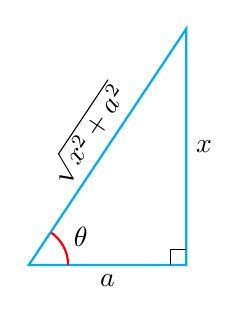
\begin{tikzpicture}[=>stealth]
\draw[thick,cyan](0,0)--(2,0)--(2,3)--cycle;
\draw(1,0)node[below]{$a$}
(2,1.5)node[right]{$x$};
\draw(1.8,0)--(1.8,0.2)--(2,0.2);
\coordinate (a) at (0.5,0);
\coordinate (b) at (0,0);
\coordinate (c) at (0.5,0.75);
\draw
pic[thick,draw=red, angle radius = 0.5cm, "$\theta$", angle eccentricity = 1.5]{angle=a--b--c};
\draw[cyan](0,0)--node[above,black,sloped]{$\sqrt{x^2 + a^2}$}(2,3);
\end{tikzpicture}
\end{figure}

\begin{align*}
\int \dfrac{dx}{\sqrt{a^2 + x^2}} & = \int \dfrac{a\sec^2\theta\hspace{0.2cm}d\theta}{\sqrt{a^2 + a^2\tan^2\theta}}\\\\
& = \int \dfrac{a\sec^2\theta \hspace{0.2cm} d\theta}{\sqrt{a^2\big(1 + \tan^2\theta\big)}} = \int \dfrac{\sec^2\theta}{\sec \theta}d\theta\\\\
& = \int \sec\theta \hspace{0.2cm}d\theta\\\\
& = \int \dfrac{\sec \theta \big(\tan \theta + \sec \theta\big)\hspace{0.2cm}d\theta}{\tan \theta + \sec\theta} = \int \dfrac{\tan \theta \sec \theta + \sec^2\theta}{\tan \theta + \sec \theta}\hspace{0.2cm}d\theta\\\\
& = \ln \left|\tan \theta + \sec \theta\right| + c\\\\
& = \ln \left|\dfrac{x}{a} + \dfrac{\sqrt{x^2 + a^2}}{a}\right| + c\\
\end{align*}

$$\text{Note:}\hspace{0.5cm} \int \sec \theta \hspace{0.2cm}d\theta = \ln\left|\tan \theta + \sec \theta\right| + c$$\\\\
\end{solution}

\begin{exa}


Find the integral $\displaystyle{\int \dfrac{dx}{x^2\sqrt{9 - x^2}}}$
\end{exa}


\begin{solution}


Let $\hspace{0.2cm} x = 3\sin \theta\hspace{0.2cm}$. Then $\hspace{0.2cm} dx = 3\cos\theta \hspace{0.2cm}d\theta\hspace{0.2cm}$. Thus

% DIAGRAM 35

\begin{figure}[H]
\centering
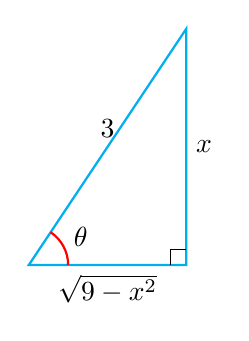
\begin{tikzpicture}[=>stealth]
\draw[thick,cyan](0,0)--(2,0)--(2,3)--cycle;
\draw(1,0)node[below]{$\sqrt{9-x^2}$}
(2,1.5)node[right]{$x$}
(1,1.5)node[above]{3};
\draw(1.8,0)--(1.8,0.2)--(2,0.2);
\coordinate (a) at (0.5,0);
\coordinate (b) at (0,0);
\coordinate (c) at (0.5,0.75);
\draw
pic[thick,draw=red, angle radius = 0.5cm, "$\theta$", angle eccentricity = 1.5]{angle=a--b--c};
\end{tikzpicture}
\end{figure}

\begin{align*}
\int \dfrac{dx}{x^2\sqrt{9 - x^2}} & = \int \dfrac{3\cos\theta \hspace{0.2cm}d\theta}{\big(3\sin\theta\big)^2\sqrt{9 - 9\sin^2\theta}} = \int \dfrac{\cos \theta}{3\sin^2\theta\cdot 3 \sqrt{1 - \sin^2\theta}}\hspace{0.2cm}d\theta\\\\
& = \dfrac{1}{9}\int \dfrac{1}{\sin^2\theta}\hspace{0.2cm}d\theta\\\\
& = \dfrac{1}{9}\int \csc^2\theta\hspace{0.2cm}d\theta\\\\
& = \dfrac{-1}{9}\cot \theta + c\\\\
& = \dfrac{-1}{9}\dfrac{\sqrt{9 - x^2}}{x} + c\\\\
\end{align*}
\end{solution}

\begin{exa}


Find the integral $\hspace{0.2cm}\displaystyle{ \int \dfrac{\sqrt{x^2 - 4}}{x}\hspace{0.2cm}dx}$
\end{exa}


\begin{solution}


Let $\hspace{0.2cm} x = 2\sec\theta \hspace{0.2cm}$ so that $\hspace{0.2cm} dx = 2\tan\theta\sec\theta\hspace{0.2cm}d\theta$

% DIAGRAM 36

\begin{figure}[H]
\centering
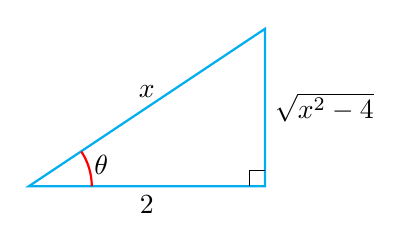
\begin{tikzpicture}[=>stealth]
\draw[thick,cyan](0,0)--(3,0)--(3,2)--cycle;
\draw(3,1)node[right]{$\sqrt{x^2 - 4}$}
(1.5,0)node[below]{2}
(1.5,1)node[above]{$x$};
\draw(2.8,0)--(2.8,0.2)--(3,0.2);
\coordinate (a) at (0.5,0);
\coordinate (b) at (0,0);
\coordinate (c) at (0.5,0.33);
\draw
pic[thick, draw = red, angle radius = 0.8cm, "$\theta$" , angle eccentricity = 1.2]{angle=a--b--c};
\end{tikzpicture}
\end{figure}

\begin{align*}
 \int \dfrac{\sqrt{x^2 - 4}}{x}\hspace{0.2cm}dx & = \int \dfrac{\sqrt{4\sec^2\theta - 4}}{2\sec \theta}\cdot 2\tan\theta \sec\theta \hspace{0.2cm} d\theta\\\\
 & = 2 \int \tan^2\theta\hspace{0.2cm} d\theta = 2\int \big(\sec^2\theta - 1\big)d\theta\\\\
 & = 2\Bigg[\int \sec^2\theta d\theta - \int d\theta \Bigg]\\\\
 & = 2\tan \theta - 2\theta + c\\\\
 & = \dfrac{2\sqrt{x^2 - 4}}{2} - 2 \sec^{-1}\Big(\dfrac{x}{2}\Big) + c=\sqrt{x^2 - 4} - 2\sec^{-1}\Big(\dfrac{x}{2}\Big) + c
\end{align*}
\end{solution}

\subsection{The Hyperbolic Substitution}
In general the following will give a guide

\begin{enumerate}
\item If the integrand involves the expression $a^2 + x^2$, substitute $x = a\sinh\theta$

\item If the integrand involves the expression $a^2 - x^2$, substitute $x = a\tanh \theta$

\item If the integrand involves the expression $x^2 - a^2$, substitute $x = a\cosh \theta$
\end{enumerate}

For the types of substitutions the most important identities to use are 
\begin{enumerate}
\item $\cosh^2\theta - \sinh^2\theta = 1$

\item $2\sinh \theta \cosh \theta = \sinh 2 \theta$

\item $\cosh^2\theta = \dfrac{1}{2}\big(1 + \cosh 2 \theta\big)$

\item $\sinh^2\theta = \dfrac{1}{2}\big( \cosh 2 \theta - 1\big)$
\end{enumerate}

\begin{exa}


Find $\displaystyle{\int \sqrt{x^2 + 1}\hspace{0.1cm}dx}$
\end{exa}


\begin{solution}


Let $\hspace{0.2cm} x = \sinh \theta\hspace{0.2cm}$. Then $\hspace{0.2cm} dx = \cosh \theta \hspace{0.1cm}d\theta$. Thus 

\begin{align*}
\int \sqrt{x^2 + 1}\hspace{0.2cm}dx & = \int \sqrt{\sinh^2 \theta + 1}\cdot \cosh\theta \hspace{0.2cm} d\theta\\\\
& = \int \sqrt{\cosh^2\theta}\cdot \cosh \theta \hspace{0.2cm}d\theta\\\\
& = \int \cosh^2 \theta \hspace{0.2cm}d\theta\\\\
& = \dfrac{1}{2}\int \big(1 + \cosh 2 \theta \big) \hspace{0.2cm}d\theta\\\\
& = \dfrac{1}{2}\Big[ \theta + \dfrac{1}{2} \sinh 2\theta \Big] + c\\\\
& = \dfrac{1}{2}\Big[\sinh^{-1}x + x\sqrt{1 + x^2}\Big] + c\\\\
\end{align*}
\end{solution}

\begin{exa}


Find $\hspace{0.3cm} \displaystyle{\int \dfrac{1}{x\sqrt{1 - x^2}}\hspace{0.2cm}dx}$
\end{exa}


\begin{solution}


Let $\hspace{0.2cm} x = \sec h\theta\hspace{0.2cm}$. Then $\hspace{0.2cm} dx = -\sec h\theta \tanh\theta \hspace{0.2cm}d\theta$


Now, $\hspace{0.2cm} 1 - x^2 = 1 - \sec h^2\theta = \tanh^2\theta$

\begin{align*}
\implies \hspace{0.5cm} \int \dfrac{1}{x\sqrt{1 - x^2}}\hspace{0.2cm}dx & = - \int \dfrac{\sec h\theta \tanh\theta\hspace{0.2cm}d\theta}{\sec h\theta \tanh\theta}\\\\
& = -\int d\theta\\\\
& = -\theta + c\\
& = -\sec h^{-1} x + c\\\\\\
\end{align*}
\end{solution}

\subsection{Integration by Partial Fractions}

\begin{exa}


Evaluate $\hspace{0.4cm} \displaystyle{I = \int \dfrac{x^4 - x^2 - 1}{x^2 (x - 1)}\hspace{0.1cm} dx}$


\begin{align*}
I & = \int \Bigg( x + \frac{2}{x} + \frac{1}{x^2} - \frac{2}{x - 1}\Bigg)\hspace{0.1cm} dx\\\\
& = \int  x\hspace{0.1cm}dx  + \int \frac{2}{x}\hspace{0.1cm}dx  + \int \frac{1}{x^2}\hspace{0.1cm}dx - \int \frac{2}{x - 1}\hspace{0.1cm}dx\\\\
& = \int  x\hspace{0.1cm}dx  + 2\int \frac{1}{x}\hspace{0.1cm}dx  + \int \frac{1}{x^2}\hspace{0.1cm}dx -2 \int \frac{1}{x - 1}\hspace{0.1cm}dx\\\\
& = \dfrac{1}{2}x^2 + 2\ln |x| - \dfrac{1}{x} - 2\ln |x - 1| + c\\\\
\end{align*}

\pagebreak
\end{exa}

\subsection{Radicals of Polynomial Expression}
Integrands involving fractional powers of polynomial expression of the form $\hspace{0.2cm} \sqrt[n]{P(x)}\hspace{0.2cm}$, make the substitution $\hspace{0.2cm} P(x) = t^n\hspace{0.2cm}$. The substitution will eliminate the radical sign since $$\hspace{0.2cm} \sqrt[n]{P(x)} = \sqrt[n]{t^n} = t$$


\begin{exa}


Find $\hspace{0.3cm}\displaystyle{ I = \int \dfrac{dx}{\sqrt{x} - \sqrt[3]{x}}\hspace{0.3cm} , \hspace{0.3cm} x>0}$
\end{exa}


\begin{solution}


Here we need to make the substitution $x = t^n$ where both $\dfrac{n}{2}$ and $\dfrac{n}{3}$ are integers.


Thus, the substitution is $\hspace{0.2cm} x = t^6\hspace{0.2cm}$ so that $\hspace{0.2cm} dx = 6t^5dt$

\begin{align*}
\implies\hspace{0.5cm} I & = \int \dfrac{6t^5}{\sqrt{t^6}- \sqrt[3]{t^6}}dt
 = 6\int \dfrac{t^5}{t^3 - t^2}dt\\\\
& = 6\int \dfrac{t^3}{t - 1}dt\\\\
& = 6\int \Big[t^2 + t + 1 + \dfrac{1}{t - 1}\Big]dt\\\\\
& = 6\Bigg[\dfrac{1}{3}t^3 + \dfrac{1}{2}t^2 + t + \ln |t - 1|\Bigg] + c\\\\
& = 6\Bigg[\frac{1}{3}x^{1/2} + \dfrac{1}{2}x^{1/3} + x^{1/6} + \ln \left|x^{1/6} - 1\right|\Bigg] + c\\\\
\end{align*}
\end{solution}

\begin{exa}


Find $\hspace{0.3cm} \displaystyle{\int \dfrac{dx}{(x- 2)\sqrt{x + 1}}}$
\end{exa}


\begin{solution}


Let $\hspace{0.2cm} x + 1 = t^2\hspace{0.2cm}$, then $\hspace{0.2cm} x = t^2 - 1$


$\therefore\hspace{0.4cm} x - 2 = t^2 - 3\hspace{0.5cm} \implies \hspace{0.5cm} dx = 2tdt$

\begin{align*}
I & = \int \dfrac{2t\hspace{0.1cm}dt}{\big(t^2 - 3\big) t}\\\\
& = 2\int \dfrac{1}{\big(t - \sqrt{3}\big)\hspace{0.1cm} \big(t + \sqrt{3}\big)}\hspace{0.1cm}dt\\\\
& = \dfrac{2}{2\sqrt{3}}\int \Bigg(\dfrac{1}{t - \sqrt{3}} - \dfrac{1}{t + \sqrt{3}}\Bigg)\hspace{0.1cm}dt\\\\
& = \frac{1}{\sqrt{3}}\Big[\ln |t - \sqrt{3}| - \ln |t + \sqrt{3}|\Big] + c\\\\
& = \dfrac{1}{\sqrt{3}}\ln\left|\dfrac{t - \sqrt{3}}{t + \sqrt{3}}\right| + c\\\\
& = \dfrac{1}{\sqrt{3}} \ln\left|\dfrac{\sqrt{x + 1} - \sqrt{3}}{\sqrt{x + 1} + \sqrt{3}}\right| + c\\\\
\end{align*}
\end{solution}

\begin{exa}


Find $\hspace{0.3cm} \displaystyle{\int \dfrac{dx}{x^2 - 6x + 13}}$
\end{exa}


\begin{solution}


We complete the square of $\hspace{0.3cm} x^2 - 6x + 13 = x^2 - 6x + 9 - 9 + 13 = \big(x - 3\big)^2 + 4$

\begin{align*}
\text{Thus}\hspace{0.5cm} I & = \int \dfrac{1}{\big(x - 3\big)^2  + 4}\hspace{0.1cm}dx\\\\
& = \dfrac{1}{2}\tan^{-1}\dfrac{x - 3}{2} + c\\\\
\end{align*}
\end{solution}

\subsection{Rational Functions of Trigonometric Functions}
The integration of any rational function of the trigonometric functions $\sin x$ and $\cos x$ can be transformed into integration of rational functions of $z$.


Let $\hspace{0.2cm} z = \tan \dfrac{x}{2}\hspace{0.2cm}$ then $\hspace{0.2cm} dz = \dfrac{1}{2}\sec^2 \Big(\dfrac{x}{2}\Big)dx$

$$\implies\hspace{0.4cm} dz = \dfrac{1}{2}\Bigg( \tan^2\Big(\dfrac{x}{2}\Big) + 1 \Bigg) dx$$


$$\implies \hspace{0.4cm}  dz = \dfrac{z^2 + 1}{2}\hspace{0.1cm} dx \hspace{0.5cm} \text{or}\hspace{0.5cm} dx = \dfrac{2}{z^2 + 1}dz$$


$\sin x$ and $\cos x$ can also be transformed as rational functions of $z$ as follows:
\begin{align*}
\cos x & = 2 \cos^2\Big(\dfrac{x}{2}\Big) - 1 = \dfrac{2}{\sec^2\Big(\dfrac{x}{2}\Big)} - 1\\
& = \dfrac{2}{1 + \tan^2\Big(\dfrac{x}{2}\Big)} - 1 \\
& = \dfrac{2}{1 + z^2} - 1\\\\
& = \dfrac{1 - z^2}{1 + z^2}\\
\end{align*}

$$\text{i.e}\hspace{0.5cm} \cos x = \dfrac{1 - z^2}{1 + z^2}\hspace{1cm} \sin x = \dfrac{2z}{1 + z^2}$$


\begin{exa}


Find $\displaystyle{\int \dfrac{dx}{2 + \cos x}}$
\end{exa}


\begin{solution}


Let $\hspace{0.2cm} z = \tan \dfrac{x}{2}\hspace{0.2cm}$, then $\hspace{0.2cm} dx = \dfrac{2}{1 + z^2}dz\hspace{0.2cm}$ and $\hspace{0.2cm} \cos x = \dfrac{1 - z^2}{1 + z^2}\hspace{0.2cm}$, thus
\begin{align*}
\int \dfrac{dx}{2 + \cos x}dx & = \int \frac{\dfrac{2}{1 + z^2}dz}{2 + \Bigg(\dfrac{1 - z^2}{1 + z^2}\Bigg)}\\
& = 2 \int \dfrac{1}{z^2 + 3}dz\\\\
& = \dfrac{2}{\sqrt{3}}\tan^{-1}\dfrac{z}{\sqrt{3}} + c\\\\
& = \dfrac{2}{\sqrt{3}}\tan^{-1}\Bigg(\dfrac{\tan (x/2)}{\sqrt{3}}\Bigg) + c\\\\
\end{align*}
\end{solution}

\subsection{The Definite Integrals}
Let $[a,b]$ be an interval on which a given function is continuous. Let $x_0, x_1 , \cdots\cdots\cdots , x_n$ be points on the interval such that $a = x_0 < x_1< x_2<\cdots\cdots\cdots < x_n = b$ and let\\ $\Delta X_k = X_k - X_{k -1}$. Then the definite integral of $f(x)$ with respect to $X$  from $X  = a$ to $X = b$ is given by $$\int^b_a f(x) dx = \lim\limits_{n \rightarrow \infty} \sum^n_{k = 1} f\big(X_k\big) \hspace{0.1cm} \Delta X_k$$


\subsection{The Fundamental Theorem of Calculus}
If $f(x)$ is continuous on the interval $[a,b]$ and if $F(x)$ is any indefinite integral of $f(x)$ then $$\int^b_a f(x) dx = F(b) - F(a)$$


\begin{note}


If $a = b$, then $\displaystyle{\int^b_a f(x) dx = 0}$.
\end{note}


\begin{exa}
Evaluate the definite integrals
\begin{enumerate}
\item $\displaystyle{\int^2_{-1}\dfrac{1}{x - 9}dx}$
\item $\displaystyle{\int_0^{\frac{2\pi}{3}} \dfrac{d \theta}{5 + 4\cos \theta}}$
\end{enumerate}
\end{exa}

\begin{solution}
\subhead{Part 1}
\begin{align*}
\int^2_{-1}\dfrac{1}{x - 9}dx &  = \ln \left|x - 9\right|\Bigg|^2_{-1}\\
& = \ln\left|2 - 9\right| - \ln \left|-1 - 9\right| = \ln 7 - \ln 10\\
& = \ln \dfrac{7}{10}\hspace{0.4cm} \text{or}\hspace{0.4cm} \ln (0.7)\\
\end{align*}

\subhead{Part 2}
Let $\hspace{0.2cm} z = \tan \dfrac{\theta}{2}\hspace{0.2cm}$ then $d \theta = \dfrac{2}{1 + z^2}dz\hspace{0.2cm}$ and $\hspace{0.2cm} \cos \theta = \dfrac{1 - z^2}{1 + z^2}\hspace{0.2cm}$ Thus

\begin{align*}
\int_0^{\dfrac{2\pi}{3}} \dfrac{d \theta}{5 + 4\cos \theta} & = \int^{\sqrt{3}}_0 \frac{\dfrac{2}{1 + z^2}}{5 + 4\Bigg(\dfrac{1 - z^2}{1 + z^2}\Bigg)}\\\\
& = 2\int^{\sqrt{3}}_0 \dfrac{1}{z^2 + 9}dz
 = \dfrac{2}{3}\tan^{-1}\dfrac{z}{3}\Bigg|^{\sqrt{3}}_0\\\\
& = \dfrac{2}{3}\tan^{\dfrac{\sqrt{3}}{3}} - \dfrac{2}{3}\tan^{-1}\dfrac{0}{3}\\\\
& = \dfrac{2}{3}\Bigg(\dfrac{\pi}{6}\Bigg) - \dfrac{2}{3}(0)\\
& = \dfrac{\pi}{9}\\\\
\end{align*}
\end{solution}

\subhead{Properties of Definite Integrals}


If $f(x)$ and $g(x)$ are continuous functions on the interval of integration $[a,b]$, then
\begin{enumerate}
\item $\displaystyle{\int^b_a  K\hspace{0.1cm} f(x) dx = K\int^b_a f(x) dx}$, $\hspace{0.2cm} K = $ constant.

\item $\displaystyle{\int^b_a \Big[ f(x)\pm g(x)\Big] dx = \int^b_a f(x) dx \pm \int^b_a g(x) dx}$

\item For $\hspace{0.2cm} a < c < b$, $\hspace{0.3cm}\displaystyle{\int^b_a f(x) dx  = \int^c_a f(x) dx   +   \int^b_c f(x) dx}$

\item $\displaystyle{\int^b_a f(x) dx = - \int^a_b f(x) dx}$

\item $\displaystyle{\int^b_a f(x) dx = (b- a) f(x_0)}\hspace{0.2cm}$
for at least one value $x = x_0$ between $a$ and $b$. This is the mean value theorem for integration.
\end{enumerate}

\subsection{Applications of Definite Integrals}

\subsubsection{Area Under the Curve}
\begin{enumerate}
\item If $f(x)$ is continuous and non-negative on the interval $[a,b]$, then the are of the region $R$ between the curve and $x-$axis is given by $$A = \int^b_a f(x) dx$$

% DIAGRAM 37

\begin{figure}[H]
\centering
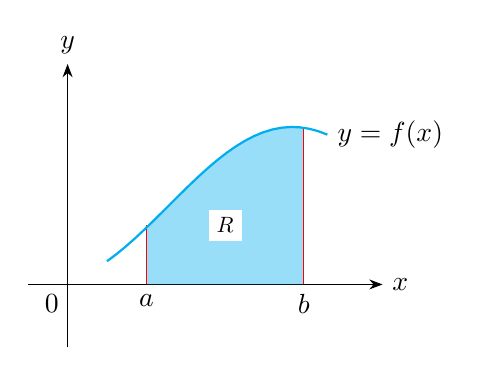
\begin{tikzpicture}[=>stealth]
\draw[-Stealth](4.5,0)--(9,0)node[right]{$x$};
\draw[-Stealth](5,-0.8)--(5,2.8)node[above]{$y$};
\path[fill=cyan,opacity=0.4,smooth,domain=6:8,variable=\x]plot(\x,{1+sin((\x)r)})--(8,2)--(8,0)--(6,0)--(6,0.7)--cycle;
\draw[red](6,0)--(6,0.75)
(8,0)--(8,2);
\draw[thick,cyan,domain=5.5:8.3,variable=\x]plot(\x,{1 + sin((\x)r)})node[right,black]{$y=f(x)$};
\draw(6,0)node[below]{$a$}
(8,0)node[below]{$b$}
(4.8,0)node[below]{$0$}
(7,0.75)node[]{$R$};
\draw(7,0.75)node[shape=rectangle,draw=white,fill=white,scale=0.8]{$R$};
\end{tikzpicture}
\end{figure}

\item If $f(x)$ is continuous and negative on the interval $[a,b]$, then the area between the curve and the $x-$axis is given by $$A = - \int^b_a f(x) dx = \int^a_b f(x) dx$$

% DIAGRAM 38

\begin{figure}[H]
\centering
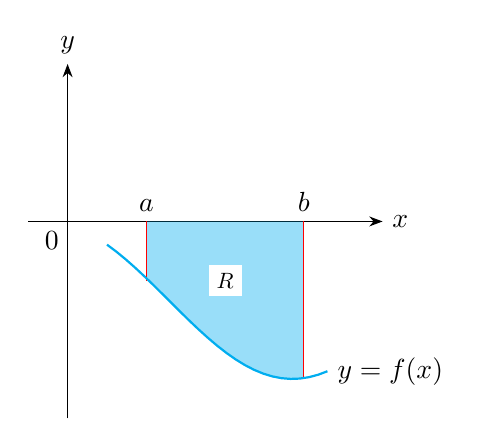
\begin{tikzpicture}[=>stealth]
\draw[-Stealth](4.5,0)--(9,0)node[right]{$x$};
\draw[-Stealth](5,-2.5)--(5,2)node[above]{$y$};
\path[fill=cyan,opacity=0.4,smooth,domain=6:8,variable=\x]plot(\x,{-1-sin((\x)r)})--(8,-2)--(8,0)--(6,0)--(6,-0.7)--cycle;
\draw[red](6,0)--(6,-0.75)
(8,0)--(8,-2);
\draw[thick,cyan,domain=5.5:8.3,variable=\x]plot(\x,{-1 - sin((\x)r)})node[right,black]{$y=f(x)$};
\draw(6,0)node[above]{$a$}
(8,0)node[above]{$b$}
(4.8,0)node[below]{$0$};
\draw(7,-0.75)node[shape=rectangle,draw=white,fill=white,scale=0.8]{$R$};
\end{tikzpicture}
\end{figure}

\end{enumerate}

\subsubsection{Area Between Two Curves}
If $f(x)$ and $g(x)$ are continuous on the interval $[a,b]$ such that $0 \leq g(x) \leq f(x)$ for  $a\leq x \leq b$, then the area $A$ of the region $R$ between the curves $y = f(x)$ and $y = g(x)$ from $x = a$ to $x = b$ is given by 
$$A = \int^b_a f(x) dx - \int^b_a g(x) dx$$

$$\text{i.e}\hspace{0.4cm} A = \int^b_a \Big[f(x) - g(x)\Big] dx$$

% DIAGRAM 39

\begin{figure}[H]
\centering
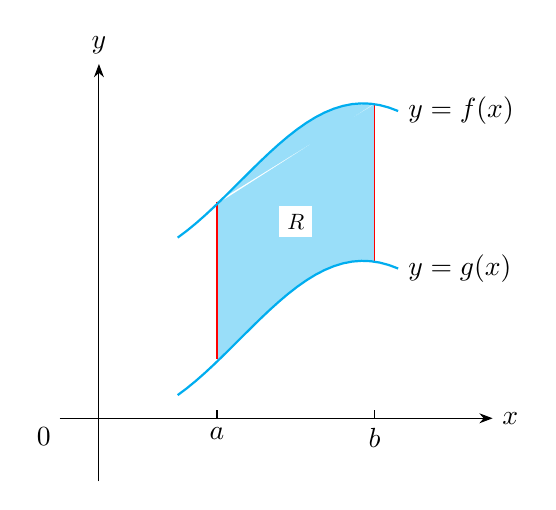
\begin{tikzpicture}[=>stealth]
\draw[-Stealth](4,0)--(9.5,0)node[right]{$x$};
\draw[-Stealth](4.5,-0.8)--(4.5,4.5)node[above]{$y$};
\path[fill=cyan,opacity=0.4,smooth,domain=6:8,variable=\x]plot(\x,{1+sin((\x)r)})--(8,2)--(8,4)--plot(\x,{3 + sin((\x)r)})--(6,2.75)--(6,0.75)--cycle;
\draw[red](6,2.75)--(6,0.75)
(8,4)--(8,2);
\draw[thick,cyan,domain=5.5:8.3,variable=\x]plot(\x,{1 + sin((\x)r)})node[right,black]{$y=g(x)$};
\draw(6,0)node[below]{$a$}
(8,0)node[below]{$b$}
(3.8,0)node[below]{$0$};
\draw(7,2.5)node[shape=rectangle,draw=white,fill=white,scale=0.8]{$R$};
\draw(8,0)--(8,0.1)
(6,0)--(6,0.1);
%%
\draw[thick,cyan,domain=5.5:8.3,variable=\x]plot(\x,{3 + sin((\x)r)})node[right,black]{$y=f(x)$};
\end{tikzpicture}
\end{figure}

\begin{exa}


Find the area of the region bounded by the curves $\hspace{0.2cm} y = x\hspace{0.2cm}$ and $\hspace{0.2cm} y = \dfrac{x^5}{16}$
\end{exa}


\begin{solution}


% DIAGRAM 40

\begin{figure}[H]
\centering
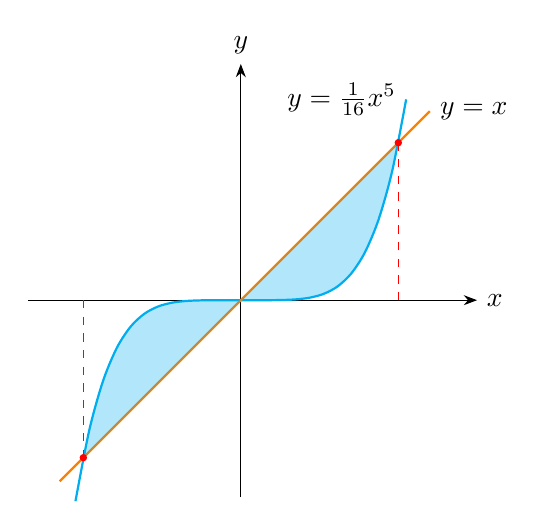
\begin{tikzpicture}[=>stealth]
\draw[-Stealth](-2.7,0)--(3,0)node[right]{$x$};
\draw[-Stealth](0,-2.5)--(0,3)node[above]{$y$};
\draw[smooth,thick,cyan,domain=-2.1:2.1,variable=\x]plot(\x,1/16*\x*\x*\x*\x*\x)node[left,black]{$y=\frac{1}{16}x^5$};
\draw[thick,orange](-2.3,-2.3)--(2.4,2.4)node[black,right]{$y=x$};
\path[fill=cyan, opacity=0.3,domain=0:2,variable=\x]plot(\x,1/16*\x*\x*\x*\x*\x)--(2,2)--(0,0)--cycle;
\path[fill=cyan, opacity=0.3,domain=-2:0,variable=\x]plot(\x,1/16*\x*\x*\x*\x*\x)--(0,0)--(-2,-2)--cycle;
\draw(2,2)node[shape=circle,fill=red,scale=0.01cm]{}
(-2,-2)node[shape=circle,fill=red,scale=0.01cm]{};
\draw[dashed,red](-2,0)--(-2,-2)
(2,0)--(2,2);
\end{tikzpicture}
\end{figure}

$x = \dfrac{x^5}{16}\hspace{0.5cm}\implies \hspace{0.5cm} x - \dfrac{x^5}{16} = 0\hspace{1cm} \implies \hspace{1cm} x\Big(1 - \dfrac{x^4}{16}\Big) = 0$


$\implies \hspace{0.4cm} x = 0  \hspace{0.2cm}$ or $\hspace{0.2cm} 1 - \dfrac{x^4}{16} = 0 \hspace{0.5cm} \implies \hspace{0.5cm} \Big(1 - \dfrac{x^2}{4}\Big)\Big( 1 + \dfrac{x^2}{4}\Big) = 0\hspace{0.3cm}$ but $1 + \dfrac{x^2}{4} \neq 0$


$\implies\hspace{0.5cm} \Big(1 - \dfrac{x}{2}\Big)\Big(1+ \dfrac{x}{2}\Big) = 0$


$\implies\hspace{0.5cm} x = -2,2$

\begin{align*}
A & = \int^0_{-2} \Bigg(\dfrac{x^5}{16} - x\Bigg) dx + \int^2_0 \Bigg( x - \dfrac{x^5}{16}\Bigg) dx\\\\
& = \Bigg(\dfrac{x^6}{96} - \dfrac{x^2}{2}\Bigg|^0_{-2} + \Bigg(\dfrac{x^2}{2} - \dfrac{x^6}{96}\Bigg|^2_0\\\\
& = -\dfrac{64}{96} + \dfrac{4}{2} + \dfrac{4}{2} - \dfrac{64}{96}\\
& = \dfrac{8}{3}\hspace{0.2cm}\text{Squared Units}\\\\
\end{align*}

\pagebreak
\end{solution}
\subsubsection{Volume of the Solid of Revolution}
When the region below the curve $y = f(x)$  between $x = a$ and $x = b$ is rotated about the $x-$axis the solid generated is called the solid of revolution and its value is called the volume of revolution.

% DIAGRAM 41

\begin{align*}
V & \approx \sum^n_{i= 1} \pi \Big[f\big(X_j\big)\Big]^2\Delta X\\\\
\implies \hspace{1cm} V &= \lim\limits_{\Delta X \rightarrow 0} \sum^{\infty}_{i = 1} \pi \Big[f(x)\Big]^2 \Delta X
= \pi \int^b_a \Big[f(x)\Big]^2 dx
\end{align*}

Therefore, the  volume of the solid of revolution is given by $$V = \pi \int^b_a \Big[f(x)\Big]^2\hspace{0.1cm} dx$$ 
when the region between the curve and the $y-$axis from $y = c$ to $y=d$ is rotated about the $y-$axis, the volume of revolution is given by $$V = \pi \int^d_c x^2\hspace{0.1cm} dy\hspace{0.4cm},\hspace{0.2cm} x = g(y)$$

% DIAGRAM 42

\begin{figure}[H]
\centering
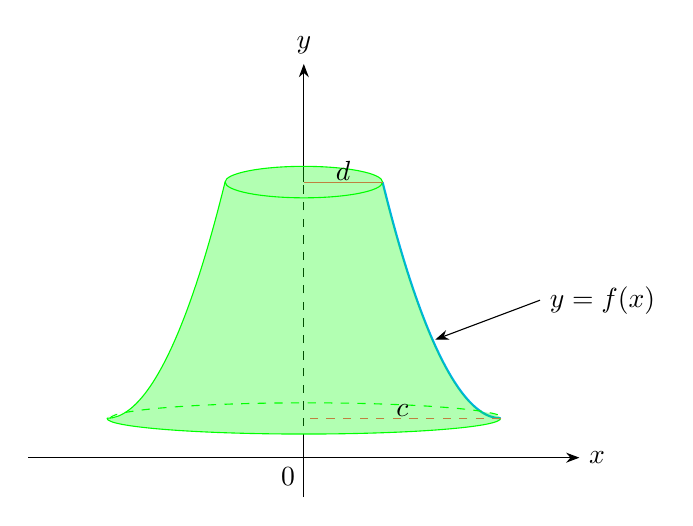
\begin{tikzpicture}[=>stealth]
\draw[-Stealth](-3.5,0)--(3.5,0)node[right]{$x$};
\draw[-Stealth](0,3.5)--(0,5)node[above]{$y$};
\draw[dashed](0,0.4)--(0,3.5);
\draw(0,-0.5)--(0,0.3);
\draw[thick,cyan](2.5,0.5)parabola(1,3.5);
\draw[green](-2.5,0.5)parabola(-1,3.5);
\draw[green](0,3.5)ellipse[x radius = 1cm, y radius = 0.2cm];
%\draw[dashed](0,0.5)circle(2.5cm and 0.2cm);
\draw[green](-2.5,0.5)arc(180:360:2.5cm and 0.2cm);
\draw[dashed,green](-2.46,0.5)arc(179:0:2.5cm and 0.2cm);
\path[fill=green,opacity=0.3](0,0.5)circle(2.5cm and 0.2cm)--(2.5,0.5)parabola(1,3.5)--(0,3.5)ellipse[x radius =1cm, y radius=0.2cm]--(-1,3.5)parabola[bend at end](-2.5,0.5)--(-2.5,0.5)arc(180:90:2.5cm and 0.2cm);
\draw[brown](1,3.5)--(0,3.5);
\draw[dashed,brown](2.5,0.5)--(0,0.5);
\draw(0.5,3.4)node[above]{$d$}
(1.25,0.4)node[above]{$c$}
(-0.2,0)node[below]{0}
(3,2)node[right]{$y=f(x)$};
\draw[-Stealth](3,2)--(1.67,1.5);
\end{tikzpicture}
\end{figure}

\begin{exa}


Find the volume of revolution generated by rotating the region bounded by the hyperbola $x^2 - y^2 = 1$, the lines $y = -2$ and $y = 2$ about the $y-$axis.
\end{exa}


\begin{solution}
\begin{align*}
V & = \int^d_c x^2\hspace{0.1cm}dy = \pi \int^2{-2} \Big(1 + y^2)dy\\
& = \pi \Bigg( y  + \dfrac{y^3}{3}\Bigg|^2_{-2}\\
% & = \pi \Bigg( 2 + \dfrac{8}{3} + 2 + \dfrac{8}{3}\Bigg)\\
& = \dfrac{28}{3}\pi\hspace{0.2cm}\text{cubic units}\\\\
\end{align*}
\end{solution}

\subhead{Washer Method}


This method is useful when the axis of rotation is not part of the boundary of the plane area.\\ If the axis of rotation is the $x-$axis, the upper boundary of the plane area is given by $y = f(x)$, and the region runs from $x = a$ to $x = b$, then Volume $V$ of the solid of revolution is given by $$V = \pi \int^b_a \Big\{ \Big[f(x)\Big]^2 - \Big[g(x)\Big]^2\Big\} dx$$

Similarly, if the axis of rotation is the $y-$axis, and the plane area is bounded the right by $x = f(y)$, to the left by $x = g(y)$ above by $y = c$ and below by $y = d$, the volume $V$ of the solid of revolution is given by 
$$V = \pi \int^d_c \Big\{ \Big[f(y)\Big]^2 - \Big[g(y)\Big]^2\Big\} dy$$

% DIAGRAM 43

\begin{figure}[H]
\centering
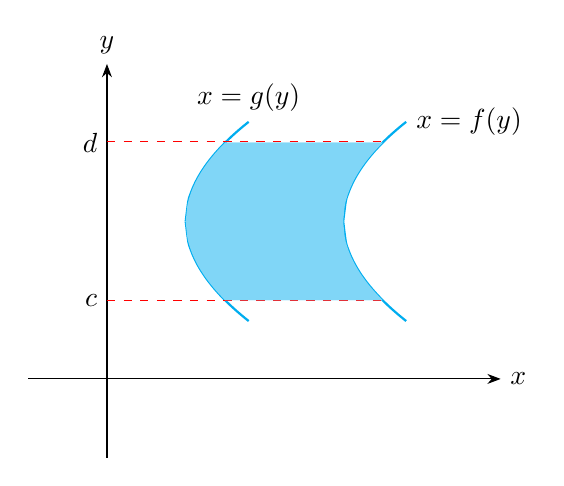
\begin{tikzpicture}[=>stealth]
\draw[-Stealth](-1,0)--(5,0)node[right]{$x$};
\draw[-Stealth](0,-1)--(0,4)node[above]{$y$};
\draw[thick,cyan,smooth,domain=1:1.8,variable=\x]plot(\x,{2+sqrt(2*(\x-1))})node[above,black]{$x=g(y)$};
\draw[thick,cyan,smooth,domain=1:1.8,variable=\x]plot(\x,{2-sqrt(2*(\x-1))});
%%%
\draw[thick,cyan,smooth,domain=3:3.8,variable=\x]plot(\x,{2+sqrt(2*(\x-3))})node[right,black]{$x=f(y)$};
\draw[thick,cyan,smooth,domain=3:3.8,variable=\x]plot(\x,{2-sqrt(2*(\x-3))});
\draw[dashed,red](0,1)--(3.5,1)
(0,3.02)--(3.5,3.02);
\draw(0,1)node[left]{$c$}
(0,3)node[left]{$d$};
\path[fill=cyan!50,domain=1:1.5,variable=\x]plot(\x,{2+sqrt(2*(\x-1))})--(1.5,3)--(3.5,3)--(1.5,1)--(1,2)--cycle;
\path[fill=cyan!50,smooth,domain=1:1.5,variable=\x]plot(\x,{2-sqrt(2*(\x-1))})--(1.5,1)--(3.5,1)--(1.5,3)--(1,2)--cycle;
\path[fill=cyan!50,smooth,domain=3:3.5,variable=\x]plot(\x,{2+sqrt(2*(\x-3))})--(3.5,3)--(1.5,3)--(1.5,1)--(3,2)--cycle;
\path[fill=cyan!50,smooth,domain=3:3.5,variable=\x]plot(\x,{2-sqrt(2*(\x-3))})--(3.5,1)--(1.5,1)--(1.5,3)--(3,2)--cycle;
\end{tikzpicture}
\end{figure}

\subhead{Shell Method}


If the axis of rotation is the $y-$axis and the plane are in the first quadrant is bounded below by  the $x-$axis above by $y = f(x)$, to the left by $x = a$ and the right by $x = b$ then volume $V$ of the solid of revolution is given by 
$$V = 2\pi \int^b_a xy\hspace{0.1cm}  dx = 2\pi \int^b_a xf(x) \hspace{0.1cm} dx$$

% DIAGRAM 44

\begin{figure}[H]
\centering
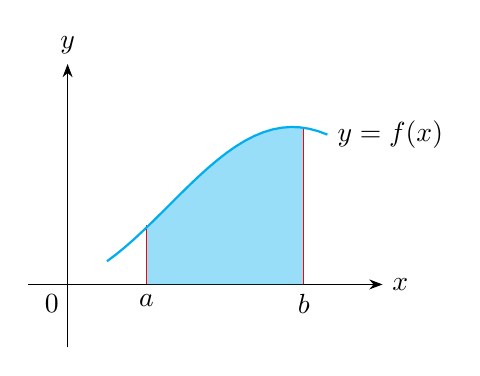
\begin{tikzpicture}[=>stealth]
\draw[-Stealth](4.5,0)--(9,0)node[right]{$x$};
\draw[-Stealth](5,-0.8)--(5,2.8)node[above]{$y$};
\path[fill=cyan,opacity=0.4,smooth,domain=6:8,variable=\x]plot(\x,{1+sin((\x)r)})--(8,2)--(8,0)--(6,0)--(6,0.7)--cycle;
\draw[red](6,0)--(6,0.75)
(8,0)--(8,2);
\draw[thick,cyan,domain=5.5:8.3,variable=\x]plot(\x,{1 + sin((\x)r)})node[right,black]{$y=f(x)$};
\draw(6,0)node[below]{$a$}
(8,0)node[below]{$b$}
(4.8,0)node[below]{$0$};
\end{tikzpicture}
\end{figure}

Similarly, if the axis of rotation is the $x-$axis and the plane area in the first quadrant is bounded to the left by the $y-$axis, to the right by $x = f(y)$ below by $y = c$ and above by $y = d$ then  the Volume $V$ of the solid of revolution is given by 
$$V = 2\pi \int^d_c xy\hspace{0.1cm}  dy = 2\pi \int^d_c yf(y) \hspace{0.1cm} dy$$

% DIAGRAM 45

\begin{figure}[H]
\centering
\begin{tikzpicture}[=>stealth]
\draw[-Stealth](-1,0)--(5,0)node[right]{$x$};
\draw[-Stealth](0,-1)--(0,4)node[above]{$y$};
\draw[thick,cyan,smooth,domain=2:2.8,variable=\x]plot(\x,{2+sqrt(2*(\x-2))})node[right,black]{$x=f(y)$};
\draw[thick,cyan,smooth,domain=2:2.8,variable=\x]plot(\x,{2-sqrt(2*(\x-2))});
\draw[dashed,red](0,1)--(2.5,1)
(0,3.02)--(2.5,3.02);
\draw(0,1)node[left]{$c$}
(0,3)node[left]{$d$}
(2.5,1)node[shape=circle,fill=cyan,draw=cyan,scale=0.01cm]{}
(2.5,3.02)node[shape=circle,fill=cyan,draw=cyan,scale=0.01cm]{};
\end{tikzpicture}
\end{figure}

\subsection{The Length of a Plane Curve}
Suppose the curve over the closed interval $[a,b]$ is given by $y = f(x)$. Let\\ $a = x_0 < x_1 < \cdots\cdots\cdots < x_n = b$ be a partition of the interval $[a,b]$. Let $P_j$ be the point on the curve whose coordinates are $(x_j , f(x_j))$ and let $S_n$ be the polygonal path obtained by joining the points $P_j, \hspace{0.2cm} j = 0, 1, 2,\cdots\cdots\cdots, n$ by straight line segments on the curve.

% DIAGRAM 46

\begin{figure}[H]
\centering
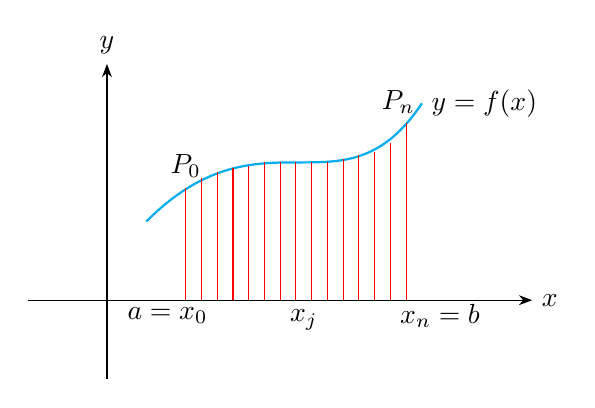
\begin{tikzpicture}[=>stealth]
\draw[-Stealth](-1,0)--(5.4,0)node[right]{$x$};
\draw[-Stealth](0,-1)--(0,3)node[above]{$y$};
\draw[thick,cyan](0.5,1)..controls(2,2.5)and (3,1)..(4,2.5);
\draw[red](1,0)--(1,1.43);
\draw[red](3.8,0)--(3.8,2.25);
\draw[red](2.6,0)--(2.6,1.75)
(2.4,0)--(2.4,1.75)
(2.2,0)--(2.2,1.75)
(2,0)--(2,1.75)
(1.8,0)--(1.8,1.7)
(1.6,0)--(1.6,1.68)
(1.4,0)--(1.4,1.63)
(1.2,0)--(1.2,1.55)
(2.8,0)--(2.8,1.75)
(3,0)--(3,1.79)
(3.2,0)--(3.2,1.84)
(3.4,0)--(3.4,1.88)
(3.6,0)--(3.6,2);
\draw(1.4,-0.2)node[left]{$a=x_0$}
(1,1.43)node[above]{$P_0$}
(3.6,-0.2)node[right]{$x_n=b$}
(3.7,2.25)node[above]{$P_n$}
(4,2.5)node[right]{$y=f(x)$}
(2.5,0)node[below]{$x_j$};
\end{tikzpicture}
\end{figure}

If we let $\max \Delta x_j \longrightarrow 0$, the polygonal path $S_n$ is almost a smooth curve. Thus, the length $S$ of a smooth curve $y = f(x)$ from $x = a$ to $x = b$ is approximately 
$$S \approx \lim\limits_{\max \Delta x_j\rightarrow 0} \sum^n_{j=1} \sqrt{\big(x_j - x_{j-1}\big)^2 + \big(f(x_j)- f(x_{j-1})\big)^2}$$

If $f(x)$ is continuous in $(a,b)$, then by the mean value theorem there exist $x^*_j \in \big(x_{j-1}, x_j\big) \ni f(x_j) - f(x_{j-1}) = f'(x_j)\big(x_j - x_{j-1}\big)$

$$ S = \int^b_a \sqrt{1 + \Big[f'(x)\Big]^2}\hspace{0.2cm}dx$$
Which is the arc length formula.


\begin{exa}


Find the length of the arc defined by $y = x^2$ from $x = 0$ to $x = 0.5$


\pagebreak
\end{exa}
\begin{solution}


% DIAGRAM 47

\begin{figure}[H]
\begin{tikzpicture}[=>stealth]
\draw[-Stealth](-3,0)--(3,0)node[right]{$x$};
\draw[-Stealth](0,-0.5)--(0,3)node[above]{$y$};
\draw[thick,cyan, smooth, domain=-2.1:2.1,variable=\x]plot(\x,1/2*\x*\x)node[right,black]{$y = f(x)$};
\draw[thick,red, dashed](1.5,0)--(1.5,1.125);
\draw(1.5,0)node[below,scale=0.8]{0.5};
\end{tikzpicture}
\end{figure}

$\displaystyle{\dfrac{dy}{dx} = 2x \hspace{0.5cm} \implies \hspace{0.5cm} \sqrt{1 + \Bigg(\dfrac{dy}{dx}\Bigg)^2 } = \sqrt{1 + 4x^2}}\hspace{0.4cm}$ Thus


$$S =  \int^{0.5}_0 \sqrt{1 + 4x^2}\hspace{0.1cm} dx = 2\int^{0.5}_0 \sqrt{\dfrac{1}{4} + x^2}\hspace{0.2cm} dx$$

Let $\hspace{0.2cm} x = \dfrac{1}{2}\tan \theta\hspace{0.2cm}$ so that $\hspace{0.2cm} dx = \dfrac{1}{2}\sec^2\theta d \theta$

\begin{align*}
\implies\hspace{0.5cm} S & = 2\int \sqrt{\dfrac{1}{4} + \dfrac{1}{4}\tan^2\theta}\cdot \dfrac{1}{2}\sec^2\theta \hspace{0.1cm}d\theta\\\\
& = \dfrac{1}{2}\int_0^{\dfrac{\pi}{4}}\sqrt{1 + \tan^2\theta}\cdot \sec^2\theta\hspace{0.1cm}d\theta\\\\
& = \dfrac{1}{2}\int_0^{\dfrac{\pi}{4}} \sec^3\theta \hspace{0.1cm}d\theta\\
\end{align*}

$$\int \sec^3\theta \hspace{0.1cm}d\theta = \dfrac{1}{2}\Big[\sec \theta \tan \theta + \ln |\sec \theta + \tan \theta | \Big]$$

\begin{align*}
\implies\hspace{0.5cm} S & = \dfrac{1}{2}\Bigg[\dfrac{1}{2}\Big[\sec \theta \tan \theta + \ln |\sec \theta + \tan \theta |\Big] \Bigg]^{\dfrac{\pi}{4}}_0\\
& = \dfrac{1}{4}\Big[\sqrt{2} + \ln \Big|1 + \sqrt{2}\Big|\Big]\\
\end{align*}

It can also be shown that the length of an arc whose equation is given in parametric form $x = f(t)$ and $y = g(t)$ for $t_1 \leq t \leq t_2$ is given by $$S = \int^{t_2}_{t_1} \sqrt{\Big[f'(t)\Big]^2 + \Big[g'(t)\Big]^2}\hspace{0.2cm} dt$$
\end{solution}


\begin{exa}


Find the length of the arc defined parametricaly by $x = \ln \sqrt{1 + t^2}\hspace{0.2cm}, \hspace{0.3cm} y = \tan^{-1}t\hspace{0.2cm}$ from $t = 0$ to $t = 1$
\end{exa}


\begin{solution}
$$f'(t) = \dfrac{dx}{dt} = \dfrac{1}{\sqrt{1 + t^2}}\cdot \Big(1 + t^2\Big)^{-1/2}\cdot t= \frac{t}{1 + t^2}$$


$$g'(t) = \dfrac{dy}{dt} = \frac{1}{1 + t^2}$$


$$\implies\hspace{0.5cm} \Big[f'(t)\Big]^2 + \Big[g'(t)\Big]^2 = \Bigg(\dfrac{t}{1 + t^2}\Bigg)+ \Bigg(\dfrac{t}{1 + t^2}\Bigg)  = \frac{t^2 + 1}{\Big(1 + t^2\Big)^2} = \dfrac{1}{1 + t^2}$$


$$\sqrt{\Big[f'(t)\Big]^2 + \Big[g'(t)\Big]^2} = \sqrt{\dfrac{1}{1 + t^2}} = \dfrac{1}{\sqrt{1 + t^2}}$$


$$\implies \hspace{0.5cm} S = \int^1_0 \dfrac{1}{\sqrt{1 + t^2}}dt$$

Let $\hspace{0.2cm} t = \tan \theta\hspace{0.2cm}$ so that $\hspace{0.2cm} dt = \sec^2\theta d\theta$

\begin{align*}
\implies\hspace{0.5cm} S & = \int^{\dfrac{\pi}{4}}_0 \dfrac{1}{\sqrt{1 + \tan^2\theta}}\cdot \sec^2\theta \hspace{0.1cm}d\theta\\
& =  \int^{\dfrac{\pi}{4}}_0\sec \theta \hspace{0.2cm}d\theta\\
& = \ln \left|\sec \theta + \tan \theta\right|\Bigg]_0^{\dfrac{\pi}{4}}\\
& = \ln\left|\sqrt{2} + 1\right|\\\\
\end{align*}
\end{solution}

\subsection{Area of Surface of Revolution}

% DIAGRAM 49

When an arc of a curve is revolved about an axis it generates a surface called the surface of revolution.


If an arc of the curve $y = f(x)$ from $x = a$ to $x = b$, is revolved about the $x-$axis, its area of surface of revolution is given by $$S_{AREA} = 2\pi \int^b_a y \hspace{0.1cm} \sqrt{1 + \Bigg(\dfrac{dy}{dx}\Bigg)^2}\hspace{0.1cm} dx$$
provided $y = f(x)$ and $f'(x)$ are continuous and $f(x)$ does not need to change sign on  the interval.


\begin{exa}


Find the area of the surface of revolution generated by revolving one loop of $8y^2 = x^2(1 - x^2)$ about the $x-$axis.

% DIAGRAM 49

\begin{figure}[H]
\centering
\begin{tikzpicture}[=>stealth]
\draw[-Stealth](-3,0)--(3,0)node[right]{$x$};
\draw[-Stealth](0,-2)--(0,2)node[above]{$y$};
\draw[smooth,domain=-2:2,thick,cyan,variable=\x]plot(\x,{1/2*sqrt(1/8*(\x*\x*(4-\x*\x)*(4-\x*\x)))});
\draw[smooth,domain=-2:2,thick,cyan,variable=\x]plot(\x,{-1/2*sqrt(1/8*(\x*\x*(4-\x*\x)*(4-\x*\x)))});
\draw[-Stealth](1.8,1.2)..controls(1.7,1.2)and(1.2,0.7)..(1.2,0.6);
\draw(1.8,1.2)node[right]{$8y^2=x^2(1-x^2)$};
\end{tikzpicture}
\end{figure}
\end{exa}

\begin{solution}


We find the $x-$axis intercepts $\hspace{0.2cm} x^2 (1 - x)^2 = 0$


$\implies\hspace{0.5cm} x = -1,\hspace{0.3cm} 0, \hspace{0.3cm}  1$


$y  = \dfrac{x \sqrt{1 - x^2}}{2\sqrt{2}}$

\begin{align*}
\implies\hspace{0.5cm} \dfrac{dy}{dx} & = \dfrac{1}{2\sqrt{2}}\Bigg(\frac{1}{2} x (1 - x^2)^{\dfrac{-1}{2}}(-2x) + (1 - x^2)^{\dfrac{1}{2}}\Bigg)\\\\
& = \frac{1 - 2x^2}{2\sqrt{2}\big(1 - x^2\big)^{\dfrac{1}{2}}}\\
\end{align*}

\begin{align*}
\implies \hspace{0.5cm} 1 + \Bigg(\dfrac{dy}{dx}\Bigg)^2  & = 1 + \dfrac{\Big(1 - 2x^2\Big)^2}{8\Big(1 - x^2\Big)} = \frac{4x^4 - 12x^2 + 9}{8\Big( 1 - x^2\Big)}\\\\
& = \frac{\Big(2x^2 - 3\Big)^2}{8\Big(1 - x^2\Big)}\\
\end{align*}

\begin{align*}
\implies \hspace{0.5cm} \sqrt{ 1 + \Bigg(\dfrac{dy}{dx}\Bigg)^2} & = \sqrt{\dfrac{\Big(2x^2 - 3\Big)^2}{8\Big(1 - x^2\Big)}}\\\\
& = \dfrac{-2x^2 + 3}{2\sqrt{2}\sqrt{1 - x^2}}\\
\end{align*}

\begin{align*}
\text{Thus}\hspace{0.5cm} S_{AREA} & = 2\pi \int_0^1 \dfrac{x \sqrt{1 - x^2}}{2\sqrt{2}} \cdot \dfrac{-2x^2 + 3}{2\sqrt{2}\sqrt{1 - x^2}}\hspace{0.2cm}dx\\\\
& = \dfrac{\pi}{4}\int^1_0 \Big(2x^3 + 3x\Big)dx = \dfrac{\pi}{4}\Bigg[-\dfrac{x^4}{2} + \dfrac{3}{2}x^2\Bigg|^1_0\\\\
& = \dfrac{\pi}{4}\Bigg[-\dfrac{1}{2} + \dfrac{3}{2}\Bigg]\\\\
& = \dfrac{\pi}{4}\hspace{0.2cm}\text{units squared}\\
\end{align*}

\begin{align*}
S_{AREA} & = 2\pi \int^d_c x\hspace{0.1cm} \sqrt{1 + \Bigg(\dfrac{dx}{dy}\Bigg)^2}\hspace{0.2cm}dy\hspace{1cm},\hspace{0.3cm} c\leq y \leq d\\
\text{or}&\\
& = 2\pi \int^b_a x\hspace{0.1cm} \sqrt{1 + \Bigg(\dfrac{dy}{dx}\Bigg)^2}\hspace{0.2cm}dx\hspace{1cm},\hspace{0.3cm} a\leq x \leq b\\\\
\end{align*}
\end{solution}

\begin{exa}


Find the area of the surface generated by revolving the arc $y = \dfrac{1}{2}x^2\hspace{0.2cm}$ from $x = 0$ to $x = 3$.

% DIAGRAM 50

\begin{figure}[H]
\centering
\begin{tikzpicture}[=>stealth]
\draw[-Stealth](-3,0)--(3,0)node[right]{$x$};
\draw[-Stealth](0,-0.5)--(0,3)node[above]{$y$};
\draw[thick,cyan, smooth, domain=-2.3:2.3,variable=\x]plot(\x,1/2*\x*\x);
\draw[red](0,0.5)--(1,0.5)--(1,0)
(0,2)--(2,2)--(2,0);
\draw(2,0)node[scale=0.9,below]{$b$}
(0,2)node[scale=0.9,left]{$d$}
(1,0)node[below,scale=0.9]{$a$}
(0,0.5)node[left,scale=0.9]{$c$};
\end{tikzpicture}
\end{figure}
\end{exa}

\begin{solution}


$\displaystyle{S_{AREA} =  2\pi \int^b_a x\hspace{0.1cm} \sqrt{1 + \Bigg(\dfrac{dy}{dx}\Bigg)^2}\hspace{0.2cm}dx}$


$\displaystyle{\dfrac{dy}{dx}  = x \hspace{0.5cm} \implies \hspace{0.5cm} 1 + \Bigg(\dfrac{dy}{dx}\Bigg)^2 = 1 + x^2 }$


$\displaystyle{\implies \hspace{0.5cm} \sqrt{1 + \Bigg(\dfrac{dy}{dx}\Bigg)^2} = \sqrt{ 1 + x^2}}$


Thus $\displaystyle{S_{AREA} = 2\pi \int^3_0 x\sqrt{1 + x^2}\hspace{0.2cm}dx}$


Let $u = 1 + x^2 \hspace{0.5cm} \implies \hspace{0.5cm} du = 2x dx\hspace{0.2cm}$ or $\hspace{0.2cm} xdx = \dfrac{1}{2}u$

\begin{align*}
\therefore\hspace{0.5cm} S_{AREA} & = 2\pi \int^{10}_1u^{1/2}\hspace{0.1cm} \dfrac{1}{2}du\\
& = \pi \int^{10}_1 u^{1/2}du = \pi \Bigg[ \dfrac{2}{3}u^{3/2}\Bigg|^{10}_1\\\\
& = \dfrac{2}{3}\pi \Big[10^{3/2} - 1 \Big]\hspace{0.2cm} \text{sq units}\\
\end{align*}

\pagebreak
\end{solution}

\subsection{Practice Problems}

These are the tutorial questions for this section, worked in full.

\begin{problem}
Find the indefinite integrals.
$$(a)\ \int\frac{dx}{5-2x}\hspace{0.7cm}
(b)\ \int xe^{3x^2}dx\hspace{0.7cm}
(c)\ \int\frac{x^2}{\sqrt{4x^3-5}}dx\hspace{0.7cm}
(d)\ \int\frac{2x+1}{4x^2+4x+3}dx$$
$$(e)\ \int\frac{\ln\left|x\right|}{x}dx\hspace{0.7cm}
(f)\ \int x\sqrt{2x^2+1}\,dx\hspace{0.7cm}
(g)\ \int\frac{\cos x}{1+\sin x}dx\hspace{0.7cm}
(h)\ \int\frac{\sin^{-1}x}{\sqrt{1-x^2}}dx$$
\end{problem}
\begin{solution}
Every one is a substitution, and in each case the substitution is the inner
function whose derivative already stands in the numerator, up to a constant.

\subhead{(a)} $u = 5-2x$, $du = -2\,dx$:
$-\dfrac12\displaystyle\int\frac{du}{u} = -\frac12\ln\left|5-2x\right| + c$.

\subhead{(b)} $u = 3x^2$, $du = 6x\,dx$:
$\dfrac16\displaystyle\int e^u du = \frac{e^{3x^2}}{6} + c$.

\subhead{(c)} $u = 4x^3-5$, $du = 12x^2dx$:
$\dfrac{1}{12}\displaystyle\int u^{-1/2}du = \frac{\sqrt{4x^3-5}}{6} + c$.

\subhead{(d)} The derivative of the denominator is $8x+4 = 4(2x+1)$, so with
$u = 4x^2+4x+3$,
$\dfrac14\displaystyle\int\frac{du}{u} = \frac14\ln\big(4x^2+4x+3\big) + c$.
No absolute value is needed: the quadratic has discriminant $16-48<0$ and is
always positive.

\subhead{(e)} $u = \ln\left|x\right|$, $du = \dfrac{dx}{x}$:
$\displaystyle\int u\,du = \frac{\big(\ln\left|x\right|\big)^2}{2} + c$.

\subhead{(f)} $u = 2x^2+1$, $du = 4x\,dx$:
$\dfrac14\displaystyle\int\sqrt u\,du = \frac{\big(2x^2+1\big)^{3/2}}{6} + c$.

\subhead{(g)} $u = 1+\sin x$, $du = \cos x\,dx$:
$\displaystyle\int\frac{du}{u} = \ln\left|1+\sin x\right| + c$.

\subhead{(h)} $u = \sin^{-1}x$, $du = \dfrac{dx}{\sqrt{1-x^2}}$:
$\displaystyle\int u\,du = \frac{\big(\sin^{-1}x\big)^2}{2} + c$.
\end{solution}

\begin{problem}
Evaluate by parts.
$$(a)\ \int x^2\sin x\,dx\hspace{0.6cm}(b)\ \int\cos^{-1}x\,dx
\hspace{0.6cm}(c)\ \int e^x\sin x\,dx\hspace{0.6cm}(d)\ \int t^2e^{-t}dt$$
$$(e)\ \int x\big(\ln x\big)^2dx\hspace{1cm}(f)\ \int x^2\tan^{-1}x\,dx
\hspace{1cm}(g)\ \int\ln\big(1+u^2\big)du$$
\end{problem}
\begin{solution}
\subhead{(a)} Two applications, differentiating the polynomial each time:
$$\int x^2\sin x\,dx = -x^2\cos x + 2\int x\cos x\,dx
= -x^2\cos x + 2x\sin x + 2\cos x + c .$$

\subhead{(b)} Take $u = \cos^{-1}x$, $dv = dx$:
$$x\cos^{-1}x + \int\frac{x}{\sqrt{1-x^2}}dx = x\cos^{-1}x - \sqrt{1-x^2} + c .$$

\subhead{(c)} Applying parts twice returns the original integral. Writing
$I = \int e^x\sin x\,dx$,
$$I = e^x\sin x - \int e^x\cos x\,dx
= e^x\sin x - \Big[e^x\cos x + \int e^x\sin x\,dx\Big]
= e^x\big(\sin x - \cos x\big) - I ,$$
so $2I = e^x(\sin x - \cos x)$ and
$I = \dfrac{e^x\big(\sin x-\cos x\big)}{2} + c$.

\subhead{(d)}
$\displaystyle\int t^2e^{-t}dt = -\big(t^2+2t+2\big)e^{-t} + c$, again by two
applications.

\subhead{(e)} With $u = (\ln x)^2$, $dv = x\,dx$:
$$\frac{x^2}{2}\big(\ln x\big)^2 - \int x\ln x\,dx
= \frac{x^2}{2}\big(\ln x\big)^2 - \frac{x^2}{2}\ln x + \frac{x^2}{4} + c
= \frac{x^2}{4}\Big[2\big(\ln x\big)^2 - 2\ln x + 1\Big] + c .$$

\subhead{(f)} With $u = \tan^{-1}x$, $dv = x^2dx$:
$$\frac{x^3}{3}\tan^{-1}x - \frac13\int\frac{x^3}{1+x^2}dx
= \frac{x^3}{3}\tan^{-1}x - \frac{x^2}{6} + \frac16\ln\big(1+x^2\big) + c ,$$
using $\dfrac{x^3}{1+x^2} = x - \dfrac{x}{1+x^2}$.

\subhead{(g)} With the logarithm as $u$ and $dv = du$:
$$u\ln\big(1+u^2\big) - \int\frac{2u^2}{1+u^2}du
= u\ln\big(1+u^2\big) - 2u + 2\tan^{-1}u + c .$$
\end{solution}

\begin{problem}
Verify the reduction formulae, and evaluate each for $n=2$, $m=3$.
$$(a)\ \int\cos^nx\,dx = \frac1n\cos^{n-1}x\sin x + \frac{n-1}{n}\int\cos^{n-2}x\,dx$$
$$(b)\ \int x^ne^xdx = x^ne^x - n\int x^{n-1}e^xdx$$
$$(c)\ \int x^m\big(\ln x\big)^ndx = \frac{x^{m+1}}{m+1}\big(\ln x\big)^n
- \frac{n}{m+1}\int x^m\big(\ln x\big)^{n-1}dx$$
\end{problem}
\begin{solution}
\subhead{(a)}
Write $\cos^nx = \cos^{n-1}x\cdot\cos x$ and integrate by parts with
$u = \cos^{n-1}x$, $dv = \cos x\,dx$:
$$\int\cos^nx\,dx = \cos^{n-1}x\sin x + (n-1)\int\cos^{n-2}x\sin^2x\,dx .$$
Replacing $\sin^2x = 1-\cos^2x$,
$$= \cos^{n-1}x\sin x + (n-1)\int\cos^{n-2}x\,dx - (n-1)\int\cos^nx\,dx .$$
Collecting the original integral on the left gives $n\int\cos^nx\,dx$ equal to
the stated right-hand side, and dividing by $n$ finishes it.

\subhead{(b)}
Immediate from parts with $u = x^n$, $dv = e^xdx$.

\subhead{(c)}
Parts with $u = (\ln x)^n$, $dv = x^mdx$ gives
$$\frac{x^{m+1}}{m+1}\big(\ln x\big)^n
- \frac{n}{m+1}\int x^{m+1}\big(\ln x\big)^{n-1}\frac{dx}{x},$$
and $\dfrac{x^{m+1}}{x} = x^m$, which is the formula. Note the last exponent is
$n-1$, not $n-2$ as printed in some copies.

\subhead{The case $n=2$, $m=3$}
From (a): $\displaystyle\int\cos^2x\,dx = \frac{\cos x\sin x}{2} + \frac{x}{2} + c$.

From (b): $\displaystyle\int x^2e^xdx = x^2e^x - 2\int xe^xdx
= \big(x^2-2x+2\big)e^x + c$.

From (c) with $m=3$, $n=2$:
$$\int x^3\big(\ln x\big)^2dx = \frac{x^4}{4}\big(\ln x\big)^2
- \frac12\int x^3\ln x\,dx
= \frac{x^4}{4}\big(\ln x\big)^2 - \frac{x^4}{8}\ln x + \frac{x^4}{32} + c .$$
\end{solution}

\begin{problem}
Given $I_n = \displaystyle\int\big(\ln x\big)^ndx$, show that
$I_n = x\big(\ln x\big)^n - nI_{n-1}$ for $n\geq 1$, and hence evaluate
$\displaystyle\int_1^2\big(\ln x\big)^3dx$.
\end{problem}
\begin{solution}
\subhead{The reduction}
Parts with $u = (\ln x)^n$ and $dv = dx$ gives
$$I_n = x\big(\ln x\big)^n - \int x\cdot n\big(\ln x\big)^{n-1}\frac{dx}{x}
= x\big(\ln x\big)^n - n\int\big(\ln x\big)^{n-1}dx
= x\big(\ln x\big)^n - nI_{n-1} .$$

\subhead{The definite integral}
Starting from $I_0 = x$ and applying the reduction,
$$I_1 = x\ln x - x,\qquad
I_2 = x\big(\ln x\big)^2 - 2\big(x\ln x - x\big),$$
$$I_3 = x\big(\ln x\big)^3 - 3\Big[x\big(\ln x\big)^2 - 2x\ln x + 2x\Big].$$
Evaluating between $1$ and $2$, and writing $L = \ln 2$, the value at $x=1$ is
$-3(0-0+2) = -6$ and at $x=2$ it is $2L^3 - 3\big(2L^2 - 4L + 4\big)$. Hence
$$\int_1^2\big(\ln x\big)^3dx = 2L^3 - 6L^2 + 12L - 6 \approx 0.1345 ,$$
where $L = \ln 2$.
\end{solution}

\begin{problem}
Use $x = \sin^2t$ and a reduction formula to evaluate
$\displaystyle\int_0^1x(1-x)^{3/2}dx$.
\end{problem}
\begin{solution}
With $x = \sin^2 t$ we have $dx = 2\sin t\cos t\,dt$ and
$1-x = \cos^2t$, so $(1-x)^{3/2} = \cos^3t$. The limits $x=0,1$ become
$t = 0, \dfrac{\pi}{2}$, and
$$\int_0^1x(1-x)^{3/2}dx
= \int_0^{\pi/2}\sin^2t\cdot\cos^3t\cdot 2\sin t\cos t\,dt
= 2\int_0^{\pi/2}\sin^3t\cos^4t\,dt .$$
The power of $\sin$ is odd, so substitute $w = \cos t$:
$$2\int_0^{\pi/2}\big(1-\cos^2t\big)\cos^4t\sin t\,dt
= 2\int_0^1\big(1-w^2\big)w^4dw
= 2\Big[\frac{w^5}{5} - \frac{w^7}{7}\Big]_0^1
= 2\Big(\frac15-\frac17\Big) = \frac{4}{35}.$$
\end{solution}

\begin{problem}
Find the unknown coefficients.
$$(a)\ \int x^4e^{3x}dx = e^{3x}\big(a_0x^4 + a_1x^3 + a_2x^2 + a_3x + a_4\big)$$
$$(b)\ \int x^2\ln^3x\,dx = x^3\big(a_0\ln^3x + a_1\ln^2x + a_2\ln x + a_3\big)$$
\end{problem}
\begin{solution}
\subhead{(a)}
Differentiate the assumed form and match. Repeated use of the reduction
$\int x^ne^{3x}dx = \dfrac{x^ne^{3x}}{3} - \dfrac{n}{3}\int x^{n-1}e^{3x}dx$
gives
$$a_0 = \frac13,\quad a_1 = -\frac49,\quad a_2 = \frac49,
\quad a_3 = -\frac{8}{27},\quad a_4 = \frac{8}{81}.$$

\subhead{(b)}
Using the reduction of the previous question with $m=2$,
$$a_0 = \frac13,\quad a_1 = -\frac13,\quad a_2 = \frac29,
\quad a_3 = -\frac{2}{27}.$$
Both may be checked by differentiating the stated right-hand side and confirming
the original integrand reappears.
\end{solution}

\begin{problem}
Find the indefinite integrals.
$$(a)\ \int\sin^2\theta\,d\theta\hspace{0.6cm}(b)\ \int\sin^2x\cos^4x\,dx
\hspace{0.6cm}(c)\ \int\frac{dx}{\sin^26x}$$
$$(d)\ \int\sin^23x\sin^25x\,dx\hspace{1.2cm}(e)\ \int\tan^5x\cos x\,dx$$
\end{problem}
\begin{solution}
\subhead{(a)}
$\sin^2\theta = \dfrac{1-\cos 2\theta}{2}$, so the integral is
$\dfrac{\theta}{2} - \dfrac{\sin 2\theta}{4} + c$.

\subhead{(b)}
Both powers are even, so use double angles. Since
$\sin x\cos x = \dfrac{\sin 2x}{2}$,
$$\sin^2x\cos^4x = \big(\sin x\cos x\big)^2\cos^2x
= \frac{\sin^22x}{4}\cdot\frac{1+\cos 2x}{2}
= \frac{\big(1-\cos 4x\big)\big(1+\cos 2x\big)}{16}.$$
Expanding and using
$\cos 4x\cos 2x = \dfrac{\cos 6x + \cos 2x}{2}$,
$$= \frac{1}{16}\Big[1 + \frac{\cos 2x}{2} - \cos 4x - \frac{\cos 6x}{2}\Big],$$
so the integral is
$$\frac{x}{16} + \frac{\sin 2x}{64} - \frac{\sin 4x}{64}
- \frac{\sin 6x}{192} + c .$$

\subhead{(c)}
$\dfrac{1}{\sin^26x} = \csc^26x$, whose integral is
$-\dfrac{\cot 6x}{6} + c$.

\subhead{(d)}
$$\sin^23x\sin^25x = \frac{1-\cos 6x}{2}\cdot\frac{1-\cos 10x}{2}
= \frac{1 - \cos 6x - \cos 10x + \cos 6x\cos 10x}{4},$$
and $\cos 6x\cos 10x = \dfrac{\cos 16x + \cos 4x}{2}$, so the integral is
$$\frac{x}{4} - \frac{\sin 6x}{24} - \frac{\sin 10x}{40}
+ \frac{\sin 16x}{128} + \frac{\sin 4x}{32} + c .$$

\subhead{(e)}
$\tan^5x\cos x = \dfrac{\sin^5x}{\cos^4x}$. The power of $\sin$ is odd, so with
$w = \cos x$,
$$-\int\frac{\big(1-w^2\big)^2}{w^4}dw
= -\int\Big(w^{-4} - 2w^{-2} + 1\Big)dw
= \frac{1}{3w^3} - \frac{2}{w} - w + c ,$$
that is
$\dfrac{1}{3\cos^3x} - \dfrac{2}{\cos x} - \cos x + c$.
\end{solution}

\begin{problem}
Integrate.
$$(a)\ \int\frac{dx}{\big(4-x^2\big)^{3/2}}\hspace{0.6cm}
(b)\ \int\frac{\sqrt{25-x^2}}{x}dx\hspace{0.6cm}
(c)\ \int\sqrt{x^2+4}\,dx$$
$$(d)\ \int\sqrt{x^2-4}\,dx\hspace{0.6cm}
(e)\ \int\frac{dx}{\sqrt{x^2-4x+13}}\hspace{0.6cm}
(f)\ \int\frac{dx}{\big(4x-x^2\big)^{3/2}}$$
\end{problem}
\begin{solution}
\subhead{(a)} Put $x = 2\sin\theta$, so $\sqrt{4-x^2} = 2\cos\theta$ and
$dx = 2\cos\theta\,d\theta$:
$$\int\frac{2\cos\theta\,d\theta}{8\cos^3\theta}
= \frac14\int\sec^2\theta\,d\theta = \frac{\tan\theta}{4}
= \frac{x}{4\sqrt{4-x^2}} + c .$$

\subhead{(b)} Put $x = 5\sin\theta$:
$$\int\frac{5\cos\theta}{5\sin\theta}5\cos\theta\,d\theta
= 5\int\frac{1-\sin^2\theta}{\sin\theta}d\theta
= 5\int\big(\csc\theta - \sin\theta\big)d\theta ,$$
giving $\sqrt{25-x^2} - 5\ln\left|\dfrac{5+\sqrt{25-x^2}}{x}\right| + c$.

\subhead{(c)} Put $x = 2\tan\theta$:
$$\int\sqrt{x^2+4}\,dx = \frac{x\sqrt{x^2+4}}{2}
+ 2\ln\left|x+\sqrt{x^2+4}\right| + c .$$

\subhead{(d)} Put $x = 2\sec\theta$:
$$\int\sqrt{x^2-4}\,dx = \frac{x\sqrt{x^2-4}}{2}
- 2\ln\left|x+\sqrt{x^2-4}\right| + c .$$

\subhead{(e)} Complete the square first:
$x^2-4x+13 = (x-2)^2+9$, so
$$\int\frac{dx}{\sqrt{(x-2)^2+9}}
= \ln\left|x-2+\sqrt{x^2-4x+13}\right| + c .$$

\subhead{(f)} Again complete the square:
$4x-x^2 = 4-(x-2)^2$. With $u = x-2$ this is part (a), giving
$$\frac{x-2}{4\sqrt{4x-x^2}} + c .$$
\end{solution}


\begin{problem}
Evaluate by partial fractions.
$$(a)\ \int\frac{dx}{x^2-9}\hspace{1cm}
(b)\ \int\frac{x^2-3x-1}{x^3+x^2-2x}dx\hspace{1cm}
(c)\ \int\frac{x\,dx}{x^2-3x-4}\hspace{1cm}
(d)\ \int\frac{x^2+3x-4}{x^2-2x-8}dx$$
\end{problem}
\begin{solution}
\subhead{(a)}
$\dfrac{1}{x^2-9} = \dfrac{1}{6}\Big(\dfrac{1}{x-3} - \dfrac{1}{x+3}\Big)$, so
the integral is
$\dfrac16\ln\left|\dfrac{x-3}{x+3}\right| + c$.

\subhead{(b)}
The denominator factors as $x(x-1)(x+2)$, and
$$\frac{x^2-3x-1}{x(x-1)(x+2)}
= \frac{1}{2x} - \frac{1}{x-1} + \frac{3}{2(x+2)},$$
so the integral is
$$\frac12\ln\left|x\right| - \ln\left|x-1\right|
+ \frac32\ln\left|x+2\right| + c .$$

\subhead{(c)}
The denominator is $(x-4)(x+1)$, and
$\dfrac{x}{(x-4)(x+1)} = \dfrac{4}{5(x-4)} + \dfrac{1}{5(x+1)}$, giving
$$\frac45\ln\left|x-4\right| + \frac15\ln\left|x+1\right| + c .$$

\subhead{(d)}
The degrees are equal, so divide first:
$$\frac{x^2+3x-4}{x^2-2x-8} = 1 + \frac{5x+4}{(x-4)(x+2)}
= 1 + \frac{4}{x-4} + \frac{1}{x+2},$$
and the integral is
$x + 4\ln\left|x-4\right| + \ln\left|x+2\right| + c$.
\end{solution}

\begin{problem}
Evaluate.
$$(a)\ \int\frac{\sqrt x}{1+x}dx\hspace{0.5cm}
(b)\ \int\frac{dx}{3+\sqrt{x+2}}\hspace{0.5cm}
(c)\ \int\frac{dx}{x\sqrt{x^2+x-1}}\hspace{0.5cm}
(d)\ \int\frac{\sqrt{4x-x^2}}{x^3}dx$$
\end{problem}
\begin{solution}
\subhead{(a)} Put $x = w^2$, $dx = 2w\,dw$:
$$\int\frac{w}{1+w^2}2w\,dw = 2\int\frac{w^2}{1+w^2}dw
= 2\int\Big(1 - \frac{1}{1+w^2}\Big)dw = 2w - 2\tan^{-1}w ,$$
that is $2\sqrt x - 2\tan^{-1}\sqrt x + c$.

\subhead{(b)} Put $w = \sqrt{x+2}$, so $x = w^2-2$ and $dx = 2w\,dw$:
$$\int\frac{2w}{3+w}dw = 2\int\Big(1 - \frac{3}{3+w}\Big)dw
= 2w - 6\ln\left|3+w\right| ,$$
that is $2\sqrt{x+2} - 6\ln\big(3+\sqrt{x+2}\big) + c$.

\subhead{(c)} Substitute $w = \dfrac1x$, so $x = \dfrac1w$ and
$dx = -\dfrac{dw}{w^2}$. Then
$$x\sqrt{x^2+x-1} = \frac1w\sqrt{\frac{1}{w^2} + \frac1w - 1}
= \frac{1}{w^2}\sqrt{1 + w - w^2}\quad (w>0),$$
so the integral becomes
$$-\int\frac{dw}{\sqrt{1+w-w^2}}
= -\int\frac{dw}{\sqrt{\frac54 - \big(w-\frac12\big)^2}}
= -\sin^{-1}\!\left(\frac{2w-1}{\sqrt5}\right) + c ,$$
that is
$-\sin^{-1}\!\left(\dfrac{2-x}{x\sqrt5}\right) + c$.

\subhead{(d)} Put $x = 4\sin^2\theta$, so
$\sqrt{4x-x^2} = 4\sin\theta\cos\theta$ and
$dx = 8\sin\theta\cos\theta\,d\theta$:
$$\int\frac{4\sin\theta\cos\theta}{64\sin^6\theta}8\sin\theta\cos\theta\,d\theta
= \frac12\int\frac{\cos^2\theta}{\sin^4\theta}d\theta
= \frac12\int\cot^2\theta\csc^2\theta\,d\theta
= -\frac{\cot^3\theta}{6}.$$
Since $\sin^2\theta = \dfrac{x}{4}$ gives
$\cot\theta = \sqrt{\dfrac{4-x}{x}}$, the answer is
$$-\frac16\left(\frac{4-x}{x}\right)^{3/2} + c .$$
\end{solution}

\begin{problem}
Evaluate.
$$(a)\ \int\frac{dx}{1+\sin x-\cos x}\hspace{0.5cm}
(b)\ \int\frac{dx}{3-2\cos x}\hspace{0.5cm}
(c)\ \int\sec x\,dx\hspace{0.5cm}
(d)\ \int\frac{dx}{5+4\sin x}$$
\end{problem}
\begin{solution}
Parts (a), (b) and (d) are rational in $\sin x$ and $\cos x$, so use the
Weierstrass substitution $t = \tan\dfrac x2$, under which
$$\sin x = \frac{2t}{1+t^2},\qquad \cos x = \frac{1-t^2}{1+t^2},
\qquad dx = \frac{2\,dt}{1+t^2}.$$

\subhead{(a)} The denominator becomes
$$1 + \frac{2t}{1+t^2} - \frac{1-t^2}{1+t^2} = \frac{2t^2+2t}{1+t^2},$$
so the integral is
$$\int\frac{1+t^2}{2t(t+1)}\cdot\frac{2\,dt}{1+t^2}
= \int\frac{dt}{t(t+1)} = \ln\left|\frac{t}{t+1}\right| + c
= \ln\left|\frac{\tan\frac x2}{1+\tan\frac x2}\right| + c .$$

\subhead{(b)} The denominator becomes
$\dfrac{3+3t^2-2+2t^2}{1+t^2} = \dfrac{1+5t^2}{1+t^2}$, so
$$\int\frac{2\,dt}{1+5t^2} = \frac{2}{\sqrt5}\tan^{-1}\big(\sqrt5\,t\big) + c
= \frac{2}{\sqrt5}\tan^{-1}\!\Big(\sqrt5\tan\frac x2\Big) + c .$$

\subhead{(c)} The standard trick is faster: multiply above and below by
$\sec x + \tan x$, whose derivative is the resulting numerator:
$$\int\frac{\sec x\big(\sec x+\tan x\big)}{\sec x+\tan x}dx
= \ln\left|\sec x + \tan x\right| + c .$$

\subhead{(d)} The denominator becomes
$\dfrac{5+5t^2+8t}{1+t^2}$, so
$$\int\frac{2\,dt}{5t^2+8t+5}
= \int\frac{2\,dt}{5\Big[\big(t+\frac45\big)^2 + \frac{9}{25}\Big]}
= \frac{2}{3}\tan^{-1}\!\left(\frac{5t+4}{3}\right) + c ,$$
that is
$\dfrac23\tan^{-1}\!\left(\dfrac{5\tan\frac x2 + 4}{3}\right) + c$.
\end{solution}

\begin{problem}
Evaluate the definite integrals.
$$(a)\ \int_{-1}^{1}\big(2x^2-x^3\big)dx\hspace{0.7cm}
(b)\ \int_{-2}^{2}e^{-x/2}dx\hspace{0.7cm}
(c)\ \int_{-5}^{-3}\sqrt{x^2-4}\,dx\hspace{0.7cm}
(d)\ \int_0^{2\pi/3}\frac{d\theta}{5+\cos\theta}$$
\end{problem}
\begin{solution}
\subhead{(a)} $x^3$ is odd, so its integral over the symmetric interval is $0$;
$2x^2$ is even, so
$$\int_{-1}^{1}2x^2dx = 2\int_0^12x^2dx = \frac43 .$$
Noticing the symmetry avoids the work.

\subhead{(b)}
$\Big[-2e^{-x/2}\Big]_{-2}^{2} = -2e^{-1} + 2e = 2\Big(e - \dfrac1e\Big)
\approx 4.70$.

\subhead{(c)} The integrand is even, so this equals
$\displaystyle\int_3^5\sqrt{x^2-4}\,dx$. Using the antiderivative found above,
$$\Big[\frac{x\sqrt{x^2-4}}{2} - 2\ln\left|x+\sqrt{x^2-4}\right|\Big]_3^5
= \frac{5\sqrt{21}-3\sqrt5}{2} - 2\ln\frac{5+\sqrt{21}}{3+\sqrt5}
\approx 6.894 .$$

\subhead{(d)} With $t = \tan\dfrac{\theta}{2}$, the denominator becomes
$\dfrac{5+5t^2+1-t^2}{1+t^2} = \dfrac{6+4t^2}{1+t^2}$, and $\theta$ running
from $0$ to $\dfrac{2\pi}{3}$ sends $t$ from $0$ to $\sqrt3$. So
$$\int_0^{\sqrt3}\frac{2\,dt}{6+4t^2}
= \frac12\int_0^{\sqrt3}\frac{dt}{\frac32+t^2}
= \frac{1}{\sqrt6}\tan^{-1}\!\frac{t\sqrt2}{\sqrt3}\Big|_0^{\sqrt3}
= \frac{\tan^{-1}\sqrt2}{\sqrt6}\approx 0.393 .$$
\end{solution}

\begin{problem}
Find the area bounded by
$$(a)\ y = 9-x^2,\ y = x+3\hspace{1.5cm}
(b)\ y = x^2-4,\ y = 8-2x^2 .$$
\end{problem}
\begin{solution}
\subhead{(a)} The curves meet where $9-x^2 = x+3$, that is
$x^2+x-6 = 0$, so $x = -3$ and $x = 2$. On that interval the parabola lies
above the line, so
$$A = \int_{-3}^{2}\Big[\big(9-x^2\big) - \big(x+3\big)\Big]dx
= \int_{-3}^{2}\big(6 - x - x^2\big)dx
= \Big[6x - \frac{x^2}{2} - \frac{x^3}{3}\Big]_{-3}^{2} = \frac{125}{6}.$$

\subhead{(b)} They meet where $x^2-4 = 8-2x^2$, that is $3x^2 = 12$ and
$x = \pm 2$. The second curve is the upper one, so
$$A = \int_{-2}^{2}\Big[\big(8-2x^2\big)-\big(x^2-4\big)\Big]dx
= \int_{-2}^{2}\big(12-3x^2\big)dx = 32 .$$
\end{solution}

\begin{problem}
Find the volume generated by revolving each region about the given line.
\begin{enumerate}
\item[(a)] Within $x^2-y^2 = 16$, $y = 0$, $x = 8$; about the $x-$axis.
\item[(b)] Within $y = 4x^2$, $x = 0$, $y = 16$; about the $y-$axis.
\item[(c)] The same region; about $y = 16$.
\item[(d)] Within $y^3 = x^4\big(1-x^2\big)$; about the $x-$axis.
\end{enumerate}
\end{problem}
\begin{solution}
\subhead{(a)} Discs of radius $y$, with $y^2 = x^2-16$, from the vertex $x=4$ to
$x=8$:
$$V = \pi\int_4^8\big(x^2-16\big)dx
= \pi\Big[\frac{x^3}{3}-16x\Big]_4^8 = \frac{256\pi}{3}.$$

\subhead{(b)} Discs perpendicular to the $y-$axis of radius $x$, with
$x^2 = \dfrac y4$:
$$V = \pi\int_0^{16}\frac{y}{4}dy = \pi\Big[\frac{y^2}{8}\Big]_0^{16} = 32\pi .$$

\subhead{(c)} Now the axis is $y = 16$, so the radius of a disc at abscissa $x$
is $16 - 4x^2$, and $x$ runs from $0$ to $2$:
$$V = \pi\int_0^2\big(16-4x^2\big)^2dx
= \pi\int_0^2\big(256 - 128x^2 + 16x^4\big)dx = \frac{4096\pi}{15}.$$

\subhead{(d)} Here $y^2 = \Big[x^4\big(1-x^2\big)\Big]^{2/3}$ and the loop runs
from $x=0$ to $x=1$, so
$$V = \pi\int_0^1x^{8/3}\big(1-x^2\big)^{2/3}dx .$$
Substituting $u = x^2$ turns this into a Beta integral,
$$V = \frac{\pi}{2}\int_0^1u^{5/6}\big(1-u\big)^{2/3}du
= \frac{\pi}{2}B\Big(\frac{11}{6},\frac53\Big)\approx 0.401 .$$
Unlike the others this does not reduce to elementary functions; the Beta
function is the honest answer.
\end{solution}

\begin{problem}
Find the arc length.
\begin{enumerate}
\item[(a)] $y^3 = 8x^2$ from $x=1$ to $x=8$
\item[(b)] $6xy = x^4+3$ from $x=1$ to $x=2$
\item[(c)] $y = \ln x$ from $x=1$ to $x=2\sqrt2$
\item[(d)] $x = e^t\cos t$, $y = e^t\sin t$ from $t=0$ to $t=4$
\end{enumerate}
\end{problem}
\begin{solution}
\subhead{(a)} $y = 2x^{2/3}$, so $y' = \dfrac{4}{3}x^{-1/3}$ and
$$1 + (y')^2 = \frac{9x^{2/3}+16}{9x^{2/3}} .$$
With $u = 9x^{2/3}+16$, $du = 6x^{-1/3}dx$, the integral becomes
$\dfrac{1}{18}\displaystyle\int\sqrt u\,du = \dfrac{u^{3/2}}{27}$, so
$$L = \frac{1}{27}\Big[\big(9x^{2/3}+16\big)^{3/2}\Big]_1^8
= \frac{52^{3/2}-125}{27} = \frac{104\sqrt{13}-125}{27}\approx 9.258 .$$

\subhead{(b)} $y = \dfrac{x^3}{6} + \dfrac{1}{2x}$, so
$y' = \dfrac{x^2}{2} - \dfrac{1}{2x^2}$ and
$$1 + (y')^2 = \Big(\frac{x^2}{2} + \frac{1}{2x^2}\Big)^2 ,$$
a perfect square, which is what makes these curves usable. Hence
$$L = \int_1^2\Big(\frac{x^2}{2}+\frac{1}{2x^2}\Big)dx
= \Big[\frac{x^3}{6} - \frac{1}{2x}\Big]_1^2 = \frac{17}{12}.$$

\subhead{(c)} $y' = \dfrac1x$, so
$$L = \int_1^{2\sqrt2}\frac{\sqrt{x^2+1}}{x}dx
= \Big[\sqrt{x^2+1} - \ln\frac{1+\sqrt{x^2+1}}{x}\Big]_1^{2\sqrt2}
= 3 - \sqrt2 + \ln\frac{1+\sqrt2}{\sqrt2}\approx 2.121 .$$

\subhead{(d)} $\dot x = e^t(\cos t - \sin t)$ and
$\dot y = e^t(\sin t + \cos t)$, so
$$\dot x^2 + \dot y^2 = e^{2t}\Big[(\cos t-\sin t)^2 + (\sin t+\cos t)^2\Big]
= 2e^{2t},$$
and
$$L = \int_0^4\sqrt2\,e^t\,dt = \sqrt2\big(e^4-1\big)\approx 75.8 .$$
\end{solution}

\begin{problem}
Find the area of the surface generated by revolving each arc about the given
axis.
\begin{enumerate}
\item[(a)] $y = \dfrac13x^3$, $0\leq x\leq 3$; about the $x-$axis
\item[(b)] the same arc; about the $y-$axis
\item[(c)] $y = \dfrac{x^3}{6} + \dfrac{1}{2x}$, $1\leq x\leq 2$; about the
$y-$axis
\item[(d)] $y = \ln x$, $1\leq x\leq 7$; about the $y-$axis
\end{enumerate}
\end{problem}
\begin{solution}
About the $x-$axis the radius is $y$; about the $y-$axis it is $x$.

\subhead{(a)} With $y' = x^2$,
$$S = 2\pi\int_0^3\frac{x^3}{3}\sqrt{1+x^4}\,dx .$$
Putting $u = 1+x^4$, $du = 4x^3dx$, this is
$\dfrac{\pi}{6}\displaystyle\int_1^{82}\sqrt u\,du$, giving
$$S = \frac{\pi}{9}\Big(82\sqrt{82}-1\Big)\approx 259.2 .$$

\subhead{(b)}
$$S = 2\pi\int_0^3x\sqrt{1+x^4}\,dx .$$
With $w = x^2$ this becomes $\pi\displaystyle\int_0^9\sqrt{1+w^2}\,dw$, so
$$S = \frac{\pi}{2}\Big(9\sqrt{82} + \sinh^{-1}9\Big)\approx 132.6 .$$

\subhead{(c)} The square root is again perfect, as in the arc length above:
$$S = 2\pi\int_1^2x\Big(\frac{x^2}{2}+\frac{1}{2x^2}\Big)dx
= 2\pi\int_1^2\Big(\frac{x^3}{2}+\frac{1}{2x}\Big)dx
= \pi\Big(\frac{15}{4} + \ln 2\Big)\approx 13.96 .$$

\subhead{(d)} With $y' = \dfrac1x$,
$$S = 2\pi\int_1^7x\sqrt{1+\frac{1}{x^2}}\,dx
= 2\pi\int_1^7\sqrt{x^2+1}\,dx
= \pi\Big(34\sqrt2 + \sinh^{-1}7 - \ln\big(1+\sqrt2\big)\Big)\approx 156.6 .$$
\end{solution}




\section{Vector Analysis}

A vector carries magnitude and direction together, which makes it the natural
language for geometry in three dimensions and for the physical quantities ---
force, velocity, acceleration --- that have both.

The section builds the algebra first. Two products are defined, and the
distinction between them is the central idea: the scalar (dot) product returns a
number and measures how far two vectors point the same way, while the vector
(cross) product returns a vector perpendicular to both and measures how far they
fail to be parallel. Between them they answer the questions of angle, projection,
area and volume, and they give clean descriptions of lines and planes in space.

The section then puts vectors in motion. A vector function traces a curve as its
parameter varies, and differentiating it yields velocity and acceleration.
Analysing that motion produces the unit tangent, normal and binormal vectors,
the curvature of a space curve, and the resolution of acceleration into
tangential and normal components --- the last of which explains why a body
moving at constant speed around a bend is nevertheless accelerating.


\subsection{Three Dimensional Coordinate System}
The Cartesian coordinates of a point $P(x,y,z)$ in space may be read from the coordinate axes by passing through $P$ perpendicular to each axis. The three coordinate planes $x = 0, \hspace{0.3cm} y = 0 $ and $z = 0$ divide the spaces into eight cells called octants. The octant in which all three coordinates are positive is called the first octant but there is no conversional numbering of the remaining seven octants. The figure below shows the first octant.

% DIAGRAM 51

\begin{figure}[H]
\centering
\begin{tikzpicture}[=>stealth]
\draw[dashed](0,0,0)--(0,0,2)
(0,0,0)--(0,2,0)
(0,0,0)--(2,0,0);
\draw[-Stealth](0,0,2)--(0,0,3);
\draw[-Stealth](0,2,0)--(0,3,0)node[above]{$z$};
\draw[-Stealth](2,0,0)--(3.5,0,0)node[right]{$y$};
\draw(0,0,3.5)node[]{$x$}
(0,2,2)node[left,scale=0.7]{$S(x,0,z)$}
(0,0,2)node[left,scale=0.7]{$(x,0,0)$}
(2,0,2)node[below,scale=0.7]{$Q(x,y,0)$}
(0,0,0)node[left,scale=0.7]{0}
(2,2,2)node[right,scale=0.7]{$P(x,y,z)$}
(2,2,0)node[right,scale=0.7]{$R(0,y,z)$}
(2,0.3,0)node[right,scale=0.7]{$(0,y,0)$}
(1,0,3.3) node[scale=0.7]{$x$ = constant}
(1.5,2.5,0)node[above,scale=0.7]{$z$ = constant};
\draw(1.7,0,1)--(2.3,0,1.3) node[right,scale=0.7]{$y=$ constant};
\draw(1,0,1.7)--(1,0,3)
(1,2,0.3)--(1.5,2.5,0);
\shade[right color=teal!50,opacity=0.2](0,2,2)--(2,2,2)--(2,2,0)--(0,2,0)--cycle;
\shade[right color=teal!60,opacity=0.3](0,0,2)--(2,0,2)--(2,0,0)--(0,0,0)--cycle;
\path[fill=teal!40,opacity=0.3](0,0,2)--(0,2,2)--(0,2,0)--(0,0,0)--cycle;
\path[fill=teal!40,opacity=0.3](0,0,0)--(2,0,0)--(2,2,0)--(0,2,0)--cycle;
\draw[brown](0,0,2)--(2,0,2)--(2,2,2);
\draw(2,2,2)node[shape=circle,fill=brown,scale=0.01cm]{};
\end{tikzpicture}
\end{figure}

The point $Q(x,y,0)$ is the projection of $P(x,y,z)$ on the $xy - $ plane. Similarly, $R(0,y,z)$ and $S(x,0,z)$ as projections of $P$ on the $yz - $ and $xz - $ planes respectively. The Cartesian product $\mathbb{R}\times \mathbb{R}\times \mathbb{R} = \{(x,y,z): x,y,z \in \mathbb{R}\}$ is the set of all ordered triples of real numbers and is denoted by $\mathbb{R}^3$. This is called the three dimensional co ordinate system. In this system an equation in $x,y,z$ represents a surface in $\mathbb{R}^3$.


\begin{exa}
\begin{enumerate}
\item What surfaces in $\mathbb{R}^3$ are represented by the following equations?
\begin{enumerate}
      \item $ z = 3$
      \item $ y = 5$
\end{enumerate}
\item Describe and sketch the surface in $\mathbb{R}^3$ represented by the equation $y = x$.
\end{enumerate}
\end{exa}

\begin{solution}
\subhead{Part 1}
\begin{enumerate}
       \item The equation $z = 3$ represents the set of $\{(x,y,z): z = 3\}$ which is the set of all points in $\mathbb{R}^3$ whose $z- $coordinates is 3. This is the horizontal plane that is parallel to the $xy - $ plane and three units above it.
       \item The equation $y = 5$ represents the set of all points in $\mathbb{R}^3$ whose $y - $ co ordinate is 5. This is the vertical plane parallel the $xz - $ plane and five units to the right of it.
\end{enumerate}

In general, if $K$ is a constant, then $x = K$ represents a plane parallel to the $yz - $ plane, $y = K$ is a plane parallel to the $xz - $ plane, $z = K$ is a plane parallel to the $xy - $ plane.

\subhead{Part 2}
The equation represents the set of all points in $\mathbb{R}^3$ whose $x - $ and $y - $ coordinates are equal, that is $\{(x,y,z): x \in \mathbb{R}, z\in \mathbb{R}\}$. This is a vertical plane that intersects the $xy - $ plane in line $y = x , z  = 0$.
\end{solution}

\begin{thm}


The distance between the origin and the point $P(x_0,y_0,z_0)$ is given by: $$d = \sqrt{x_0^2 + y_0^2 + z_0^2}$$
\end{thm}

\begin{proof}


% DIAGRAM 52

\begin{figure}[H]
\centering
\begin{tikzpicture}[=>stealth]
\draw[-Stealth](-0.5,0,0)--(2.5,0,0)node[right]{$y$};
\draw[-Stealth](0,-0.5,0)--(0,2.5,0)node[above]{$z$};
\draw[-Stealth](0,0,-1)--(0,0,3);
\draw(0,0,3.5)node[]{$x$}
(2,2,2)node[shape=circle,fill=red,scale=0.01cm]{}
(2,2,2)node[right,scale=0.7]{$P(x_0,y_0,z_0)$}
(2,1,2)node[right,scale=0.7]{$z_0$}
(2,0,1)node[right,scale=0.7]{$x_0$}
(1,0,2.5)node[scale=0.7]{$y_0$}
(1,0,1)node[left,scale=0.7]{$a$};
\draw[thick,cyan](0,0,0)--node[black,sloped,above]{$d$}(2,2,2);
\draw[dashed,red](0,0,0)--(2,0,2)
(2,0,2)--(2,2,2);
\draw[brown](0,0,2)--(2,0,2)--(2,0,0);
\draw(1.8,0,1.8)--(1.8,0.2,1.8)--(2,0.2,2);
\end{tikzpicture}
\end{figure}

From the diagram $d^2 = z_0^2 + a^2$ but $a^2 = x_0^2 + y_0^2$
\begin{align*}
\therefore\hspace{0.5cm} d^2 & = x_0^2 + y_0^2 + z_0^2\\
\implies \hspace{0.5cm} d & = \sqrt{x_0^2 + y_0^2 + z_0^2}\\
\end{align*}

Similarly, the distance between two points $P_1(x_1,y_1,z_1)$ and $P_2(x_2,y_2,z_2)$ is given by $$d = \sqrt{(x_2 - x_1)^2 +  (y_2 - y_1)^2 + (z_2 - z_1)^2             }$$

\pagebreak
\end{proof}
\subsection{Vectors}
Vectors in space are the three $-$ dimensional analog of vectors in the plane and are subject to the same rules of addition, subtraction and scalar multiplication that govern vectors in the plane. The vectors from the origin to the points $(1,0,0) , (0,1,0)$ and $(0,0,1)$ are the basic unit vectors. We denote them by $\textbf{i}, \textbf{j}$ and $\textbf{k}$, respectively. We write the vectors from the origin $O$ to the point $P(x,y,z)$ as $\overline{v} = \overrightarrow{OP} = x\textbf{i} + y\textbf{j} + z\textbf{k}$. If $P_1(x_1,y_1,z_1)$ and $P_2(x_2,y_2,z_2)$ are two points then the vectors from $P_1$ to $P_2$  is the vector $$\overrightarrow{P_1P_2} = (x_2 - x_1)\textbf{i} +  (y_2 - y_1)\textbf{j} +  (z_2 - z_1)\textbf{k}$$


The length (magnitude) of any vector $A = a\textbf{i} +  b\textbf{j} +  c\textbf{k}$ is given by $$\left|A\right| = \sqrt{a^2 + b^2 + c^2}$$\\

\subsection{Direction of a Vector}
For any non-zero vector $A$, we obtain a unit vector called the direction of $A$ by dividing $A$ by its own length, i.e $$\text{Direction of }\hspace{0.3cm} A = \frac{A}{
\left|A\right|
}$$


\subhead{Direction Cosines}


% Diagram
Let $\alpha$ be the angle between the vector $\overrightarrow{OP}$ and the positive $x -$ axis, $\beta$ the angle between the $y - $ axis and $\overrightarrow{OP}$ and $\gamma$ be the angle between the $z - $ axis and $\overrightarrow{OP}$. The angles $\alpha, \beta, \gamma$ are called the direction angle of the vector $\overrightarrow{OP}$.

$$\cos \alpha = \frac{x_0}{\sqrt{x_0^2 + y_0^2 + z_0^2}}$$

$$\cos \beta = \frac{y_0}{\sqrt{x_0^2 + y_0^2 + z_0^2}}$$

$$\cos \gamma = \frac{z_0}{\sqrt{x_0^2 + y_0^2 + z_0^2}}$$

The numbers $\cos \alpha, \cos \beta$ and $\cos \gamma$ are called the direction cosines of $\overrightarrow{OP}$.


\begin{exe}


Show that $cos^2 \alpha + \cos^2 \beta + \cos^2 \gamma = 1$.
\end{exe}


\subsection{The Scalar or Dot Product of Two Vectors}
The dot or scalar product of two non zero vectors \textbf{A} and \textbf{B} is the number $\textbf{A}\cdot\textbf{B} = \left|\textbf{A}\right|\left|\textbf{B}\right|\hspace{0.1cm}\cos \theta\hspace{0.2cm},$\\$ \hspace{0.2cm} 0 \leq \theta \leq \pi,$ where $\theta$ is the angle between $\textbf{A}$ and $\textbf{B}$. If either $\textbf{A}$ or $\textbf{B}$ is 0, we define $\textbf{A}\cdot \textbf{B}  = 0$.\\\\

\subhead{Work and the Dot Product}


Let \textbf{F} be a force which moves an object from a point $P$ to $Q$, then the work done by \textbf{F} in moving the object is defined by $$W = \left|\overrightarrow{PQ}\right|\left|\textbf{F}\right| \cos \theta$$

Note that $W = \overrightarrow{PQ}\cdot \textbf{F}$


\begin{exa}
\begin{enumerate}
\item If the vectors $\overline{a}$ and $\overline{b}$ have length 4 and 6 angle between them is $\dfrac{\pi}{3}$, find $\overline{a}\cdot\overline{b}.$
\item A crate is hauled 8$m$ up a ramp under a constant force of $200 N$ applied on an angle of $25^o$ to the ramp. Find the work done.
\end{enumerate}
\end{exa}

\begin{solution}
\begin{align*}
\overline{a}\cdot \overline{b} & = \left|\overline{a}\right|\left|b\right|\cos \theta\\
& = 4\cdot 6\cdot \cos \dfrac{\pi}{3}\\
& = 12
\end{align*}

\begin{align*}
W & = \left|\textbf{F}\right|\left|\textbf{D}\right|\cos \theta\\
& = 200 \times 8 \times \cos 25^o\\
& = 1450 N\cdot M = 1450 J\\
\end{align*}
\end{solution}

\subhead{The Dot Product in Component form}


The dot product of $\overline{a} = \langle a_1, a_2, a_3\rangle$ and $\overline{b} = \langle b_1, b_2, b_3\rangle$ is $$\overline{a}\cdot \overline{b} = a_1b_1 + a_2b_2 + a_3b_3$$

\begin{exa}
\begin{enumerate}
\item Show that $2\textbf{i} + 2\textbf{j} -\textbf{k}$ is perpendicular to $ 5\textbf{i} - 4\textbf{j} + 2\textbf{k}$.
\item Find the angle between the vectors $\overline{a} = \langle 2,2,-1\rangle$ and $\overline{b} = \langle 5, -3,2\rangle$.
\item A force is given by a vector $\textbf{F} = 3\textbf{i} + 4\textbf{j} + 5\textbf{k}$ and moves a particle from the point $P(2,1,0)$ to $Q(4,6,2)$. Find the work done.
\end{enumerate}
\end{exa}

\begin{solution}
\subhead{Part 1}
Two vectors are perpendicular if their dot product is 0 $$(2\textbf{i} + 2\textbf{j} -\textbf{k})\cdot ( 5\textbf{i} - 4\textbf{j} + 2\textbf{k}) = 10 - 8 - 2 = 0$$ 
$\therefore$ the two vectors are perpendicular.

\subhead{Part 2}
$\displaystyle{\overline{a}\cdot \overline{b} = \left|\overline{a}\right|\left|\overline{b}\right|\cos \theta \implies \cos \theta = \frac{\overline{a}\cdot\overline{b}}{
\left|\overline{a}\right|\left|\overline{b}\right|
}}$

$\displaystyle{\overline{a}\cdot\overline{b} = 2(5) - 2(3) -1(2) = 2}$

$\displaystyle{\left|\overline{a}\right| = \sqrt{9} = 3\hspace{1cm} , \hspace{1cm} \left|\overline{b}\right|= \sqrt{38}}$

\begin{align*}
\cos \theta & = \frac{2}{3\sqrt{38}}\implies \theta = \cos^{-1} \Big(\frac{2}{3\sqrt{38}}\Big) \approx 84^o\\\\
\end{align*}

\subhead{Part 3}
\begin{align*}
W & = \textbf{F}\cdot (\overrightarrow{PQ})\\
 & = (\textbf{F} = 3\textbf{i} + 4\textbf{j} + 5\textbf{k})\cdot ( 2\textbf{i} + 5\textbf{j} + 2\textbf{k})\\\\
 & = 36\\
\end{align*}
\end{solution}

\subhead{Properties of Dot Product}


If $\overline{a}, \overline{b}$ and $\overline{c}$ are vectors and $\alpha$ is a scalar, then 
\begin{enumerate}
\item $\overline{a}\cdot\overline{a} = \left|\overline{a}\right|^2$
\item $\overline{a}\cdot\overline{b} = \overline{b}\cdot\overline{a}$
\item $\overline{a}\cdot(\overline{b}+ \overline{c}) = \overline{a}\cdot \overline{b} + \overline{a}\cdot\overline{c}$
\item $(\alpha \overline{a})\cdot \overline{b} = \alpha (\overline{a}\cdot\overline{b}) = \overline{a}\cdot (\alpha \overline{b})$
\item $\overline{0}\cdot \overline{a} = \overline{a}\cdot \overline{0} = 0$
\end{enumerate}

\begin{proof}


\pagebreak
\end{proof}
\subsection{Projections}
The figure below show representations $\overrightarrow{PQ}$ and $\overrightarrow{PR}$ of two vectors $\overline{a}$ and $\overline{b}$ with the same initial point $P$.

% DIAGRAM 53

\begin{figure}[H]
\centering
\begin{tikzpicture}[=>stealth]
\draw[red](0,0.05)--(2.9,0.05)--(2.9,0.09)--(3,0)--(2.9,-0.09)--(2.9,-0.05)--(0,-0.05)--cycle;
\draw[red,dashed](3,0)--(3,2);
\draw[thick,cyan,-Stealth](0,0)--(3,2);
\draw[thick,cyan,-Stealth](0,0)--(4.5,0);
\draw(0,0)node[below,scale=0.7]{$P$}
(3,2)node[above,scale=0.7]{$R$}
(3,0)node[below,scale=0.7]{$S$}
(4.5,0)node[below,scale=0.7]{$Q$}
(1.5,-0.6)node[below,]{proj$_{\overline{a}}\hspace{0.08cm}\overline{b}$};
\draw(3.2,0)--(3.2,0.2)--(3,0.2);
\draw[-Stealth](1.5,-0.6)--(1,-0.05);
\end{tikzpicture}
\end{figure}

\hspace{1cm}

\begin{figure}[H]
\centering
\begin{tikzpicture}[=>stealth]
\draw[red](0,0.05)--(-1.9,0.05)--(-1.9,0.09)--(-2,0)--(-1.9,-0.09)--(-1.9,-0.05)--(0,-0.05)--cycle;
\draw[thick,cyan,-Stealth](0,0)--(2.5,0);
\draw[thick,cyan,-Stealth](0,0)--(-2,2);
\draw(-2.5,0)--(0,0)
(-2.2,0)--(-2.2,0.2)--(-2,0.2);
\draw[red,dashed](-2,0)--(-2,2);
\draw(-2,2)node[left,scale=0.7]{$R$}
(-2,0)node[below,scale=0.7]{$S$}
(0,0)node[below,scale=0.7]{$P$}
(2.5,0)node[below,scale=0.7]{$Q$}
(1.25,0)node[above,scale=0.9]{$\overline{a}$}
(-1,1)node[above,scale=0.9]{$\overline{b}$}
(-1,-0.6)node[below,scale=0.9]{Proj$_{\overline{a}}\hspace{0.1cm}\overline{b}$};
\draw[-Stealth](-1,-0.6)--(-1,-0.05);
\end{tikzpicture}
\end{figure}

If $S$ is the foot of the perpendicular from $R$ to the line containing $\overrightarrow{PQ}$ then the vector with representations $\overrightarrow{PS}$ is called the vector projection of $\overline{b}$ onto $\overline{a}$ and denoted by $Proj_{\overline{a}}\overline{b}$. It is given by $$Proj_{\overline{a}}\overline{b} = \frac{\overline{a}\cdot \overline{b}}\,{\left|\overline{a}\right|^2} \overline{a}
$$

The scalar projection of $\overline{b}$ onto $\overline{a}$ (also called the component of $\overline{b}$ onto $\overline{a}$) is given by $$Comp_{\overline{a}}\hspace{0.1cm}\overline{b} = \frac{\overline{a} \cdot \overline{b}}{\left|\overline{a}\right|
}$$


\subsection{Lines in Three Dimensional Space}
Let $P(x_1,y_1,z_1)$ and $Q(x_2,y_2,z_2)$ be two points on a straight line $L$ as shown below.

% DIAGRAM 54

\begin{figure}[H]
\centering
\begin{tikzpicture}[=>stealth]
\draw[-Stealth](0,0,0)--(3,0,0)node[right]{$y$};
\draw[-Stealth](0,0,0)--(0,3,0)node[above]{$z$};
\draw[-Stealth](0,0,0)--(0,0,4);
\draw(0,0,4.5)node[]{$x$}
(0,0,0)node[left]{0}
(-1,2,1)node[shape=circle,fill=red,scale=0.01cm]{}
(1,2,-1)node[shape=circle,fill=red,scale=0.01cm]{}
(2,2,-2)node[shape=circle,fill=red,scale=0.01cm]{}
(2,2,-2)node[right,scale=0.8]{$Q(x_2,y_2,z_2)$}
(0.8,2,-1)node[above,scale=0.8]{$P(x_1,y_1,z_1)$}
(-1,2,1)node[above,scale=0.8]{$R(x,y,z)$}
(-2,2,2.5)node[]{$L$};
\draw[-Stealth,thick,cyan](0,0,0)--(1,1.99,-1);
\draw[-Stealth,thick,cyan](0,0,0)--(-1,1.99,1);
\draw[thick,red](-2,2,2)--(2,2,-2);
\end{tikzpicture}
\end{figure}

The vector $\overrightarrow{PQ}$ is parallel to the line $L$. Let $R(x,y,z)$ be an arbitrary point on the line $L$. Then the vector $\overrightarrow{RP}$ is parallel to vector $\overrightarrow{PQ}$. Hence $$ \overrightarrow{PR} = t \overrightarrow{PQ}\hspace{0.5cm} \cdots\cdots\cdots\hspace{0.5cm} (I)$$
for some real number $t$. From the diagram above $\overrightarrow{OR} = \overrightarrow{OP} + \overrightarrow{PR}$ thus, $$\overrightarrow{OR} = \overrightarrow{OP} + t \overrightarrow{PQ}\hspace{0.5cm} \cdots\cdots\cdots\hspace{0.5cm} (II)$$
$(II)$ is the vector equation of a straight line which passes through the points $P$ and $Q$.


Usually, the vector equations of a straight line is written as
$$\underline{r} = \underline{P} + t \underline{P}a\hspace{0.5cm} \cdots\cdots\cdots \hspace{0.5cm} (III)$$

Now, $\overrightarrow{PQ} = (x_2 -x_1)\textbf{i} + (y_2 -y_1)\textbf{j} + (z_2 -z_1)\textbf{k}$, $\hspace{0.5cm} \overrightarrow{OR} = x \hat{i} + y\hat{j} + z\hat{k}\hspace{0.5cm}$ and $\hspace{0.5cm}\overrightarrow{OP} = x_1\hat{i} + y_1\hat{j} + z_1\hat{k}$. Thus, the vector equation of a straight line can be written as 
$$x\hat{i} + y\hat{j} + z \hat{k} = x_1 \hat{i} + y_1\hat{j} + z_1\hat{k} + t[(x_2 -x_1)\hat{i}  +   (y_2 -y_1)\hat{j}    + (z_2 -z_1)\hat{k}] \hspace{0.5cm} \cdots\cdots\cdots\hspace{0.5cm} (IV)$$ 

from $(IV)$ we have 
\[\overline{\underline{V}}
\begin{cases}
x & = x_1 + t(x_2 - x_1)\\
y & = y_1 + t(y_2 - y_1)\\
z & = z_1 + t(z_2 -z_1)\\
\end{cases}
\] 
These are the parametric equations of the straight line which passes through $P$ and $Q$. From the parametric equations making $t$ the subject of the formula, we have
$$t = \frac{x - x_1}{x_2 - x_1} =  \frac{y - y_1}{y_2 - y_1} =  \frac{z - z_1}{z_2 - z_1}$$
which is symmetric equation of straight line which passes through the points $P$ and $Q$.


The symmetric equation a straight line is usually written as 
$$\frac{x - x_1}{a} = \frac{y - y_1}{b} = \frac{z - z_1}{c}$$
where $a = x_2 -x_1\hspace{0.5cm}, \hspace{0.5cm} b = y_2 - y_1 \hspace{0.5cm} $ and $\hspace{0.5cm} c = z_2 - z_1$


\begin{note}
the vector $a\hat{i} + b\hat{j} + c\hat{k}$ is parallel to the straight line passing through the points $P$ and $Q$.
\end{note}


\begin{exa}


Find the vector equation, parametric equations and symmetric equations of a straight line which passes through the point $P(2,3,-1)$ and $Q(3,0,4)$.
\end{exa}


\begin{solution}


The vector equation of a straight line is given by 
\begin{align*}
\overrightarrow{OR} & = \overrightarrow{OP} + t \overrightarrow{PQ}\\
\underline{r} & = \underline{P} + t \overline{PQ}
\end{align*}

$\underline{r} = x\hat{i} + y\hat{j} + z\hat{k} \hspace{0.5cm}, \hspace{0.5cm} \underline{P} = 2\hat{i} + 3\hat{j} - \hat{k}\hspace{0.5cm}$ and $\hspace{0.5cm} \overrightarrow{PQ} = (3 - 2)\hat{i} + (0-3)\hat{j} + (4-(-1))\hat{k} = \hat{i} - 3\hat{j} + 5\hat{k}$


$\therefore$ the vector equation of a straight line is   $x\hat{i} + y\hat{j} + z\hat{k} = 2\hat{i} + 3\hat{j} - \hat{k} + t (\hat{i} - 3\hat{j} + 5\hat{k})$ or $\underline{r}=  2\hat{i} + 3\hat{j} - \hat{k} + t (\hat{i} - 3\hat{j} + 5\hat{k})$


The parametric equations  are\hspace{0.3cm}
$\displaystyle{
\begin{cases}
x & = 2 + t\\
y & = 3 - 3t\\
z & = -1 + 5t\\
\end{cases}}$\\\\

The symmetric equation is  \hspace{0.2cm}$\displaystyle{\frac{x-2}{1} = \frac{y - 3}{-3} = \frac{z + 1}{5}}$
\end{solution}


\begin{note}
\end{note}


The vector $\hat{\textbf{i}} - 3 \hat{\textbf{j}} + 5\hat{\textbf{k}}$ is parallel to the straight line.


Now, if $L$ is a straight line which passes through the point $(x,y,z)$ and is parallel to the vector $\underline{V} = a \hat{\textbf{i}} + b\hat{\textbf{j}} + c\hat{\textbf{k}},$ then the symmetric equation of the line is as follows:
\begin{enumerate}
\item $\displaystyle{\frac{x- x_1}{a} = \frac{y - y_1}{b} = \frac{z - z_1}{c}}$, if $a, b, c$ are all non zero.
\item $x =x_1$, $\dfrac{y - y_1}{b} = \dfrac{z - z_1}{c}$ if $a = 0$ and $b$ and $c$ are both nonzero then the line is parallel to the $yz$ plane $y = y_1,$ $\dfrac{x - x_1}{a} = \dfrac{z - z_1}{c}$.
If either $b$ or $c$ is equal to zero but $a\neq 0$ similar results hold.
\item $x =x_1, y = y_1 , z = z_1 + ct$, if $a$ and $b$ are zero and $c\neq 0$. The line is parallel to the\\ $z-$ axis. If $a$ and $c$ are zero or $b$ and $c$ are zero, the similar results hold
$$x = x_1\hspace{0.3cm} , \hspace{0.3cm} y = y_1 +bt\hspace{0.3cm} ,\hspace{0.3cm} z =z_1$$
$$x = x_1 + at\hspace{0.3cm} , \hspace{0.3cm} y = y_1\hspace{0.3cm} , \hspace{0.3cm} z = z_1$$
\end{enumerate}

\subsection{The Vector Product of Two Vectors}

\begin{defn}


Let $\underline{a}$ and $\underline{b}$ be two non parallel vectors in the same plane and let $\underline{c}$ be a third vector not in the plane of $\underline{a}$ and $\underline{b}$. Then , the three vectors $\underline{a}, \underline{b}$ and $\underline{c}$ are said to form a right handed set. If they are mutually perpendicular.

% DIAGRAM 55

\begin{figure}[H]
\centering
\begin{tikzpicture}[=>stealth]
\draw[-Stealth,thick,cyan](0,0,0)--(2,0,0);
\draw[-Stealth,thick,cyan](0,0,0)--(0,2,0);
\draw[-Stealth,thick,cyan](0,0,0)--(0,0,2);
\draw(1,0,0)node[above]{$\underline{a}$}
(0,1,0)node[left]{$\underline{c}$}
(0,0,1)node[below]{$\underline{b}$};
\end{tikzpicture}
\end{figure}

Note that by definition, the unit vectors $\textbf{i}, \textbf{j}$ and $\textbf{k}$ form a right handed set.

%DIAGRAM 56

\begin{figure}[H]
\centering
\begin{tikzpicture}
\draw[-Stealth](0,0,0)--(3,0,0)node[right]{$y$};
\draw[-Stealth](0,0,0)--(0,3,0)node[above]{$z$};
\draw[-Stealth](0,0,0)--(0,0,3);
\draw(0,0,3.5)node[]{$x$};
\draw[-Stealth,thick,teal](0,0,0)--(2,0,0)node[above,black,scale=0.7]{$\textbf{j}$};
\draw[-Stealth,thick,teal](0,0,0)--(0,2,0)node[right,black,scale=0.7]{$\textbf{k}$};
\draw[-Stealth,thick,teal](0,0,0)--(0,0,2)node[above,black,scale=0.7]{$\textbf{i}$};
\end{tikzpicture}
\end{figure}
\end{defn}

\begin{defn}


The vector product of two vectors $\underline{a}$ and $\underline{b}$ is defined as $\underline{a} \times \underline{b} = \left|a\right|\left|b\right|\sin \theta\hspace{0.1cm} \hat{\textbf{n}}$, where $\theta$ is the angle between $\underline{a}$  and $\underline{b}$ and $\hat{\textbf{n}}$ is a unit vector in the direction of $\underline{a} \times \underline{b}$. The vectors $\underline{a}$, $\underline{b}$ and $\underline{a} \times \underline{b}$ form a right handed set.\\
\end{defn}

\begin{note}
\begin{enumerate}
\item The vector (cross) product $\underline{a} \times \underline{b}$ is perpendicular to both $\underline{a}$ and $\underline{b}$.
\item $\underline{b}\times \underline{a} = -(\underline{a} \times \underline{b})$.
\end{enumerate}
\end{note}

\begin{thm}


Let $\underline{a}$ and  $\underline{b}$ be nonzero vectors. Then $\underline{a}$ and  $\underline{b}$ are parallel if and only if $\underline{a} \times \underline{b} =0$.


Using the definition of vector product we have following 
$$ \textbf{i}\times \textbf{i}= 0 \hspace{0.2cm}, \hspace{0.2cm} \textbf{i}\times \textbf{j} = \textbf{k} \hspace{0.2cm} ,\hspace{0.2cm} \textbf{i} \times \textbf{k} = - \textbf{j}\hspace{0.2cm} ,$$
$$\textbf{j} \times \textbf{i} = -\textbf{k}\hspace{0.2cm} , \hspace{0.2cm} \textbf{j} \times \textbf{j} = 0 \hspace{0.2cm} , \hspace{0.2cm}  \textbf{j} \times \textbf{k} = \textbf{i}\hspace{0.2cm}, $$
$$\textbf{k} \times \textbf{i} = \textbf{j}\hspace{0.2cm}, \hspace{0.2cm} \textbf{k} \times \textbf{j} = -\textbf{i} \hspace{0.2cm} , \hspace{0.2cm} \textbf{k} \times \textbf{k} = 0$$

The vector product of the unit vectors $\textbf{i}, \textbf{j}$ and $\textbf{k}$ form the following array.

% DIAGRAM 57

\begin{figure}[H]
\centering
\begin{tikzpicture}[=>stealth]
\draw[thick,cyan,-Stealth](0.9,0.41)arc[start angle =24.49, end angle = 90, radius=1]node[left,scale=0.7,black]{$\textbf{j}$};
\draw[thick,cyan,-Stealth](-0.3,0.95)arc[start angle = 106.699, end angle=180, radius = 1]node[below,scale=0.7,black]{$\textbf{k}$};
\draw[thick,cyan,-Stealth](-0.9,-0.41)arc[start angle=204.49, end angle=360, radius = 1]node[above, scale=0.7,black]{$\textbf{i}$};
\end{tikzpicture}
\end{figure}

The array is used to place signs in the cross product of the unit vectors $\textbf{i}$, $\textbf{j}$ and $\textbf{k}$. If in performing a cross product of two of the unit vectors, we proceed counterclockwise, then the resultant will be a third vector with a plus sign. If the direction is clockwise then the resultant will have a minus sign.
\end{thm}


\begin{thm}


For any scalar $\alpha$ and any pair of vectors $\underline{a}$ and $\underline{b}$ $$\alpha (\underline{a} \times \underline{b}) = (\alpha \underline{a}) \times \underline{b} =\underline{a} \times (\alpha \underline{b})$$

Note that taking $\alpha = -1$ gives $$-\big(\underline{a}\times \underline{b}\big) = \big(-\underline{a}\big)\times \underline{b}=\underline{a}\times \big(-\underline{b}\big).$$
\end{thm}


\begin{proof}


If $\alpha = 0$, all the products are zero. If $\alpha > 0$, $ \theta $ is an angle between $\underline{a}$ and $\underline{b}$ and $\widehat{\textbf{n}}$ is a vector in the direction of $\underline{a} \times \underline{b}$, then
\begin{align*}
\alpha (\underline{a} \times \underline{b}) & = \alpha \Big( \left|a\right|\left|b\right| \sin \theta \hspace{0.1cm}\widehat{\textbf{n}}\Big)\\
& =\Big(\alpha  \left|a\right|\left|b\right|\Big) \sin \theta \hspace{0.1cm}\widehat{\textbf{n}}\\
& = \left|\alpha a\right|\left|b\right| \sin \theta \hspace{0.1cm}\widehat{\textbf{n}}=(\alpha \underline{a} ) \times \underline{b}\\
& = \left|a\right|\left|\alpha b\right| \sin \theta \hspace{0.1cm}\widehat{\textbf{n}}= \underline{a}\times (\alpha \underline{b})
\end{align*}

If $\alpha < 0$, then $\alpha (\underline{a} \times \underline{b})$ is a vector that is parallel to $\underline{a} \times \underline{b}$ but in the opposite direction. On the hand, $\alpha \underline{a}$ is parallel to $\underline{a}$ but also points in the opposite direction. Thus $(\alpha \underline{a}) \times \underline{b}$ points in the opposite direction $(\underline{a} \times \underline{b})$.


In addition the length or the vectors $\alpha (\underline{a} \times \underline{b})$ and $(\alpha \underline{a}) \times \underline{b}$ are equal. Therefore the vectors $\alpha(\underline{a} \times \underline{b})$ and $(\alpha \underline{a})\times \underline{b}$ are equal. A similar argument shows that $\alpha(\underline{a}\times \underline{b}) = \underline{a} \times (\alpha \underline{b})$.
\end{proof}


\subhead{The Associative Law}


If $\alpha$ and $\beta$ are any two scalars, $\underline{a}$ and $\underline{b}$ vectors\,, then \hspace{0.2cm}$(\alpha \underline{a}) \times (\beta \underline{b}) = (\alpha \beta ) \underline{a} \times \underline{b}$


\subhead{The Distributive Law}


For any three vectors $\underline{a}, \underline{b}$ and $\underline{c}$\,, then\hspace{0.2cm} $\underline{a}\times (\underline{b} + \underline{c}) = (\underline{a}\times \underline{b}) + (\underline{a}\times \underline{c}$


\subhead{The Companion Law}


For any three vectors $\underline{a}, \underline{b}$ and $\underline{c}$\,, then\hspace{0.2cm}
$(\underline{b} + \underline{c})\times \underline{a} = (\underline{b} \times \underline{a}) + (\underline{c} \times \underline{a})$


\begin{thm}


If $\underline{a} = a_1 \textbf{i} + a_2 \textbf{j} + a_3\textbf{k}$ and  $\underline{b} = b_1 \textbf{i} + b_2 \textbf{j} + b_3\textbf{k}$
$$\underline{a} \times \underline{b} =
\begin{vmatrix}
\textbf{i} & \textbf{j} & \textbf{k}\\
a_1 & a_2 & a_3\\
b_1 & b_2 & b_3\\
\end{vmatrix}$$
\end{thm}

\begin{proof}
Expand the product using the distributive law, taking the scalar coefficients
outside by the scalar law stated above. This gives nine terms, one for each
pair of basis vectors:
\begin{align*}
\underline{a}\times\underline{b}
&= \big(a_1\textbf{i} + a_2\textbf{j} + a_3\textbf{k}\big)\times
   \big(b_1\textbf{i} + b_2\textbf{j} + b_3\textbf{k}\big)\\
&= a_1b_1(\textbf{i}\times\textbf{i}) + a_1b_2(\textbf{i}\times\textbf{j})
 + a_1b_3(\textbf{i}\times\textbf{k})\\
&\quad + a_2b_1(\textbf{j}\times\textbf{i}) + a_2b_2(\textbf{j}\times\textbf{j})
 + a_2b_3(\textbf{j}\times\textbf{k})\\
&\quad + a_3b_1(\textbf{k}\times\textbf{i}) + a_3b_2(\textbf{k}\times\textbf{j})
 + a_3b_3(\textbf{k}\times\textbf{k})
\end{align*}

Now evaluate the nine basis products from the definition of the cross product.
For the three like pairs the angle between the vectors is $0$, so
$\sin\theta = 0$ and
$$\textbf{i}\times\textbf{i} = \textbf{j}\times\textbf{j}
= \textbf{k}\times\textbf{k} = \underline{0}.$$
For the unlike pairs the vectors are perpendicular unit vectors, so the
magnitude is $1\cdot 1\cdot\sin 90^\circ = 1$, and the right-hand rule fixes the
direction:
$$\textbf{i}\times\textbf{j} = \textbf{k},\qquad
\textbf{j}\times\textbf{k} = \textbf{i},\qquad
\textbf{k}\times\textbf{i} = \textbf{j},$$
$$\textbf{j}\times\textbf{i} = -\textbf{k},\qquad
\textbf{k}\times\textbf{j} = -\textbf{i},\qquad
\textbf{i}\times\textbf{k} = -\textbf{j}.$$

Substituting these, the three like terms vanish and the remaining six become
\begin{align*}
\underline{a}\times\underline{b}
&= a_1b_2\textbf{k} - a_1b_3\textbf{j} - a_2b_1\textbf{k}
 + a_2b_3\textbf{i} + a_3b_1\textbf{j} - a_3b_2\textbf{i}\\
&= \big(a_2b_3 - a_3b_2\big)\textbf{i}
 - \big(a_1b_3 - a_3b_1\big)\textbf{j}
 + \big(a_1b_2 - a_2b_1\big)\textbf{k}
\end{align*}

Finally, expanding the determinant in the statement along its first row gives
$$\begin{vmatrix}
\textbf{i} & \textbf{j} & \textbf{k}\\
a_1 & a_2 & a_3\\
b_1 & b_2 & b_3\\
\end{vmatrix}
= \textbf{i}\begin{vmatrix} a_2 & a_3\\ b_2 & b_3\end{vmatrix}
- \textbf{j}\begin{vmatrix} a_1 & a_3\\ b_1 & b_3\end{vmatrix}
+ \textbf{k}\begin{vmatrix} a_1 & a_2\\ b_1 & b_2\end{vmatrix}$$
$$= \big(a_2b_3 - a_3b_2\big)\textbf{i}
 - \big(a_1b_3 - a_3b_1\big)\textbf{j}
 + \big(a_1b_2 - a_2b_1\big)\textbf{k},$$
which is the same expression. Hence the two agree.
\end{proof}

\begin{exa}
\begin{enumerate}
\item Given that $\underline{a} = 2 \textbf{i} - \textbf{j} + \textbf{k}\hspace{0.2cm},\hspace{0.2cm} \underline{b} = \textbf{i} + 2\textbf{j} - 3\textbf{k},\hspace{0.2cm}$ evaluate $\underline{a} \times \underline{b}$ and hence find $\sin \theta$.
\item Find symmetric equations of the line which passes through $(-1,1,2)$ whose direction vector is orthogonal to the direction vectors of the lines $\displaystyle{\frac{x - 2}{1} = \frac{y + 1}{2} = \frac{z - 1}{3}}$ and $\displaystyle{\frac{x - 1}{5} = \frac{y - 2}{2} = \frac{z + 1}{-3}}$
\item Find the distance of the point $P(1,2,6)$ from the line which passes through $A(3,-2,3)$ and $B(2,1,4)$.
\end{enumerate}
\end{exa}

\begin{solution}
\subhead{Part 1}
\begin{align*}
\underline{a} \times \underline{b} & = 
\begin{vmatrix}
\textbf{i} & \textbf{j} & \textbf{k}\\
2 & -1 & 1\\
1 & 2 & -3\\
\end{vmatrix}
 = \begin{vmatrix}
-1 & 1\\
2 & -3\\
\end{vmatrix}\textbf{i} - \begin{vmatrix}
2 & 1\\
1 & -3\\
\end{vmatrix}\textbf{j} + \begin{vmatrix}
2 & -1\\
1 & 2\\
\end{vmatrix}\textbf{k}\\
& = \textbf{i} + 7\textbf{j} + 5\textbf{k}
\end{align*}

$\displaystyle{ \underline{a} \times \underline{b} = \left|\underline{a}\right|\left|\underline{b}\right| \sin \theta \hspace{0.1cm} \left|\widehat{\textbf{n}}\right|}$

$$\left|\underline{a}\times \underline{b}\right| = \left||\underline{a}||\underline{b}|\sin \theta |\widehat{\textbf{n}}|\right|\hspace{0.1cm}, \hspace{0.2cm}\text{but}\hspace{0.2cm} |\widehat{\textbf{n}}| = 1$$

So that $\left|\underline{a}\times \underline{b}\right|= \left|\underline{a}\right|\left|b\right|\sin \theta$

$$\sin \theta = \frac{\left|\underline{a} \times \underline{b}\right|
}{\left|\underline{a}\right|\left|\underline{b}\right|
}$$

$$\left|\underline{a}\times \underline{b}\right|=\sqrt{75} = 5\sqrt{3}\hspace{0.5cm},\hspace{0.5cm}
 \left|\underline{a}\right|=\sqrt{6}\hspace{0.5cm},\hspace{0.5cm} \left|\underline{b}\right|=\sqrt{14}$$

$$\therefore\hspace{1cm} \sin \theta = \frac{5\sqrt{3}}{\sqrt{6}\sqrt{14}}= \frac{5}{2\sqrt{7}}$$

\subhead{Part 2}
Note that the direction vectors of the given lines are $\underline{a}  = \textbf{i} + 2\textbf{j} + 3\textbf{k}$ and $\underline{b} = 5\textbf{i} + 2\textbf{j} - 3\textbf{k}$. The  vector orthogonal to $\underline{a}$ and $\underline{b}$ 

$$\underline{a} \times \underline{b} = \begin{vmatrix}
\textbf{i} & \textbf{j} & \textbf{k}\\
1 & 2 & 3\\
5 & 2 & -3\
\end{vmatrix}= -12 \textbf{i} + 18\textbf{j} - 8\textbf{k}$$
Thus, the direction vector of the line is $ -12 \textbf{i} + 18\textbf{j} - 8\textbf{k}$. So symmetric  equations are 
$$\frac{x + 1}{-12} = \frac{y - 1}{18} = \frac{z - 2}{-8}$$

\subhead{Part 3}
% DIAGRAM 58

\begin{figure}[H]
\begin{tikzpicture}[=>stealth]
\draw[thick,cyan,-Stealth](0,0)--(2,3);
\draw[thick,cyan,-Stealth](0,0)--(3.4,0);
\draw[dashed,thick,red](2,0)--(2,3);
\draw(2.2,0)--(2.2,0.2)--(2,0.2);
\coordinate (a) at (0.5,0);
\coordinate (b) at (0,0);
\coordinate (c) at (0.5,0.75);
\draw
pic[thick, draw=red, angle radius = 0.5cm, angle eccentricity = 1.5,"$\theta$"]{angle=a--b--c};
\draw(2,1.5)node[right]{$d$}
(0,0)node[shape=circle, scale=0.01cm, fill=cyan]{}
(2,3)node[shape=circle,scale=0.01cm, fill=cyan]{}
(3.4,0)node[shape=circle, scale=0.01cm, fill=cyan]{};
\draw(0,0)node[left ,scale=0.8]{$A$(3,-2,3)}
(3.4,0)node[right,scale=0.8]{$B$(2,1,4)}
(2,3)node[above,scale=0.8]{$P$(1,2,6)}
(7,3)node[right]{
$\displaystyle{\sin \theta = \frac{d}{\left|\overrightarrow{AP}\right|
}}$}
(7,1.5)node[right]{$\displaystyle{
\overrightarrow{AP}\times \overrightarrow{AB} = \left|\overrightarrow{AP}\right|\left|\overrightarrow{AB}\right|\sin \theta}$}
(7,0)node[right]{$\displaystyle{\implies\hspace{1cm} \sin \theta = \frac{\left|\overrightarrow{AP}\times \overrightarrow{AB}\right|
}{\left|\overrightarrow{AP}\right|\left|\overrightarrow{AB}\right|
}}$};
\end{tikzpicture}
\end{figure}

\begin{align*}
d & = \left|\overrightarrow{AP}\right|\sin \theta = \left|\overrightarrow{AP}\right|\cdot
\frac{\left|\overrightarrow{AP}\times \overrightarrow{AB}\right|
}{\left|\overrightarrow{AP}\right|\left|\overrightarrow{AB}\right|
}\\
d & = 
\frac{\left|\overrightarrow{AP}\times \overrightarrow{AB}\right|
}{\left|\overrightarrow{AB}\right|
} = \frac{\sqrt{30}}{\sqrt{11}}\\
\end{align*}
\end{solution}

A geometrical interpretation of the length of the cross product can be seen by looking at the figure below.

% DIAGRAM 59

\begin{figure}[H]
\centering
\begin{tikzpicture}[=>stealth]
\path[fill=olive!30](0,0,2)--(2,0,2)--(2.5,1,0)--(0.5,1,0)--cycle;
\draw[thick,cyan,-Stealth](0,0,2)--(0.5,1,0);
\draw[thick,cyan,-Stealth](0,0,2)--(2,0,2);
\draw(0,0.3,0)node[above]{$\underline{b}$}
(1.5,0,2)node[below]{$\underline{a}$};
\draw[red, dashed](0.5,1,0)--node[right,black]{$h$}(1,0,2);
\coordinate (a) at (0.5,0,2);
\coordinate (b) at (0,0,2);
\coordinate (c) at (0.5,0.7,2);
\draw
pic[draw, angle radius =0.5cm, angle eccentricity = 1.5,"$\theta$"]{angle = a--b--c};
\end{tikzpicture}
\end{figure}

$$\sin \theta = \frac{h}{
\left|b\right|
}\implies h = \left|b\right| \sin \theta$$

$$A = \left|\underline{b}\right|\sin \theta \left|\underline{a}\right|=\left|\underline{a} \times \underline{b}\right|$$

If $\underline{a}$ and $\underline{b}$ are represented by directed line segments with the same initial point, then they determine a parallelogram with base $\left|\overline{a}\right|$, altitude $\left|\underline{b}\right|\sin \theta$ and area is $$A = \left|\underline{a}\right|\left|\underline{b}\right|\sin \theta = \left|\underline{a} \times \underline{b}\right|$$

\begin{exa}


Find the area of the triangle with vertices $P(1,4,6) , Q(-2, 5, -1)$ and $R(1,-1,1)$.
\end{exa}


\begin{solution}


$\overrightarrow{PQ} = -3\textbf{i} + \textbf{j} - 7\textbf{k}\hspace{0.2cm}, \hspace{0.2cm} \overrightarrow{PR} = -5\textbf{j} - 5\textbf{k}$

% \DIAGRAM 60

\begin{figure}[H]
\centering
\begin{tikzpicture}[=>stealth]
\path[fill=olive!30](0,0,2)--(2,0,2)--(2.5,1,0)--(0.5,1,0)--cycle;
\draw[thick,cyan,-Stealth](0,0,2)--(0.5,1,0);
\draw[thick,cyan,-Stealth](0,0,2)--(2,0,2);
\draw(0.5,1,0)node[left,scale=0.7]{$Q$}
(0,0,2)node[below,scale=0.7]{$P$}
(2,0,2)node[right,scale=0.7]{$R$}
(4,0.5,1)node[right]  {$A = \dfrac{1}{2}\left|\overrightarrow{PQ}\times \overrightarrow{PR}\right|$} ;
\draw[red](0.5,1,0)--(2,0,2);
\coordinate (a) at (0.5,0,2);
\coordinate (b) at (0,0,2);
\coordinate (c) at (0.5,0.7,2);
\draw
pic[draw, angle radius =0.5cm, angle eccentricity = 1.5,"$\theta$"]{angle = a--b--c};
\end{tikzpicture}
\end{figure}

$$\overrightarrow{PQ}\times \overrightarrow{PR} = \begin{vmatrix}
\textbf{i} & \textbf{j} & \textbf{k}\\
-3 & 1 & -7\\
0 & -5 & -5\\
\end{vmatrix} = -40\textbf{i} -15\textbf{j} + 15\textbf{k}$$

Area of triangle $PQR= \dfrac{1}{2}\left|-40\textbf{i} -15\textbf{j} + 15\textbf{k}\right| = \dfrac{5}{2}\sqrt{82}$\\\\\\\
\end{solution}

\subsection{Triple Products}
The product $\underline{a}\cdot(\underline{b}\times \underline{c})$ is called the scalar triple product of the vectors $\underline{a}, \underline{b}$ and $\underline{c}$. Its geometric significance can be seen by considering the parallel piped determined by the vectors $\underline{a}, \underline{b}$ and $\underline{c}$.


% DIAGRAM 61

\begin{figure}[H]
\centering
\begin{tikzpicture}[=>stealth]
\draw[-Stealth,thick,cyan](0,0,0)--(2,0,0);
\draw[-Stealth,thick,cyan](0,0,0)--(0,0,-4);
\draw[-Stealth,thick,cyan](0,0,0)--(1,2,0);
\draw[-Stealth,thick](0,0,0)--(0,3,0);
\path[fill=gray, opacity=0.2](1,2,0)--(3,2,0)--(3,2,-4)--(1,2,-4)--cycle;
\path[fill=gray,opacity=0.3](0,0,0)--(2,0,0)--(2,0,-4)--(0,0,-4)--cycle;
\path[fill=gray,opacity=0.2](0,0,-4)--(1,2,-4)--(3,2,-4)--(2,0,-4)--cycle;
\shade[top color=gray,opacity=0.5](2,0,0)--(3,2,0)--(3,2,-4)--(2,0,-4)--cycle;
\path[fill=gray,opacity=0.2](0,0,0)--(1,2,0)--(1,2,-4)--(0,0,-4)--cycle;
\shade[top color =gray,opacity=0.2](0,0,0)--(2,0,0)--(3,2,0)--(1,2,0)--cycle;
\path[fill=olive,opacity=0.3](-2,0,1.5)--(3.5,0,1.5)--(4,0,-4)--(2,0,-4)--(2,0,0)--(0,0,0)--(-0.79,0,-4)--(-1,0,-4)--cycle;
\draw(1.5,0,0)node[scale=0.8,below]{$\underline{b}$}
(0,0,-2.5)node[scale=0.8,right]{$\underline{c}$}
(0.8,1.6,0)node[left,scale=0.8]{$\underline{a}$}
(0,2.5,0)node[right,scale=0.8]{$\underline{a}\times\underline{b}$}
(0,1,0.4)node[scale=0.8]{$h$};
\draw[red,dashed](0,2)--(1,2);
\draw(0,2.2)--(0.2,2.2)--(0.2,2)
(0,0,0.2)--(0,0,0.6)
(0,2,0.2)--(0,2,0.6);
\coordinate (a) at (0.5,1);
\coordinate (b) at (0,0);
\coordinate (c) at (0,1);
\draw
pic[draw=black,angle radius = 0.8cm,->, "$\theta$", angle eccentricity = 1.3]{angle=a--b--c};
\draw[->](0,0.8,0.4)--(0,0,0.4);
\draw[->](0,1.2,0.4)--(0,2,0.4);
\end{tikzpicture}
\end{figure}

\begin{align*}
h & = \left|\left|\underline{a}\right|\cos \theta\right|\hspace{0.2cm}\text{Area of base}\hspace{0.2cm} = \left|\underline{b}\times \underline{c}\right|\\\\
V & = \left|\underline{a}\right|\left|\cos \theta\right|\left|\underline{b}\times \underline{c}\right|\\
& = \left|\left|\underline{a}\right|\left|\underline{b}\times \underline{c}\right|\cos \theta\right|\\
& = \left|\underline{a} \cdot (\underline{b}\times \underline{c})\right|
\end{align*}

Suppose $\underline{a}, \underline{b}$ and $\underline{c}$ are given in component form.
\begin{align*}
\underline{a} & = a_1\textbf{i} + a_2\textbf{j} + a_3\textbf{k}\\
\underline{b} & = b_1\textbf{i} + b_2\textbf{j} + b_3\textbf{k}\\
\underline{c} & = c_1\textbf{i} + c_2\textbf{j} + c_3\textbf{k}
\end{align*}
$$\text{then}\hspace{1cm}\underline{a}\cdot (\underline{b} \times \underline{c}) = \begin{vmatrix}
a_1 & a_2 & a_3\\
b_1 & b_2 & b_3\\
c_1 & c_2 & c_3
\end{vmatrix}$$

\begin{proof}
Write $\underline{b}\times\underline{c}$ in component form first. By the theorem
on the vector product,
$$\underline{b}\times\underline{c}
= \big(b_2c_3 - b_3c_2\big)\textbf{i}
- \big(b_1c_3 - b_3c_1\big)\textbf{j}
+ \big(b_1c_2 - b_2c_1\big)\textbf{k}.$$

Now take the dot product with $\underline{a}$. Since the dot product of vectors
in component form multiplies corresponding components and adds,
\begin{align*}
\underline{a}\cdot\big(\underline{b}\times\underline{c}\big)
&= a_1\big(b_2c_3 - b_3c_2\big)
 - a_2\big(b_1c_3 - b_3c_1\big)
 + a_3\big(b_1c_2 - b_2c_1\big)\\
&= a_1\begin{vmatrix} b_2 & b_3\\ c_2 & c_3\end{vmatrix}
 - a_2\begin{vmatrix} b_1 & b_3\\ c_1 & c_3\end{vmatrix}
 + a_3\begin{vmatrix} b_1 & b_2\\ c_1 & c_2\end{vmatrix}
\end{align*}

The right-hand side is precisely the cofactor expansion along the first row of
$$\begin{vmatrix}
a_1 & a_2 & a_3\\
b_1 & b_2 & b_3\\
c_1 & c_2 & c_3
\end{vmatrix},$$
which proves the claim.
\end{proof}

\begin{remark}
Two consequences are worth recording, and both follow from properties of
determinants rather than from any new geometry.

Interchanging two rows of a determinant changes its sign, so interchanging any
two of the three vectors reverses the sign of the triple product; a cyclic
permutation interchanges two rows twice and therefore leaves it unchanged:
$$\underline{a}\cdot\big(\underline{b}\times\underline{c}\big)
= \underline{b}\cdot\big(\underline{c}\times\underline{a}\big)
= \underline{c}\cdot\big(\underline{a}\times\underline{b}\big).$$

A determinant with two equal rows is zero, so the triple product vanishes
whenever two of the vectors are equal --- and, more usefully, it vanishes exactly
when the three vectors are coplanar, since a parallelepiped with zero volume is
a flat one. That is the test used in the example below.
\end{remark}


\begin{exa}


Use the scalar triple product to show that the vectors $\underline{a} = \langle 1 , 4, -7\rangle$ , $\underline{b} = \langle 2, -1, 4\rangle$ and $\underline{c} = \langle 0,-9,18\rangle$ are coplaner. i.e they lie on the same plane.
\end{exa}


\begin{solution}


If they lie on the same plane then the volume of the parallolopiped they determine.\\ i.e $\underline{a} \cdot (\underline{b}\times \underline{c}) = 0$

\begin{align*}
\underline{a} \cdot (\underline{b}\times \underline{c}) & = \begin{vmatrix}
1 & 4 & -7\\
2 & -1 & 4\\
0 & -9 & 18\\
\end{vmatrix} = 18 - 144 -7(-8)\\
& = 0
\end{align*}
$\therefore\hspace{0.6cm} \underline{a}, \underline{b}$ and $\underline{c}$ are coplaner.
\end{solution}


\begin{exa}
\begin{enumerate}
\item Find a vector equation and parametric equations for the line that passes through the point $(5,1,3)$ and is parallel to the vector $\textbf{i} + 4\textbf{j} - 2\textbf{k}$.
\item Find two other points on the line
\end{enumerate}
\end{exa}

\begin{solution}
\begin{enumerate}
\item 
\begin{align*}
\overline{r} & = \underline{P} + t\overrightarrow{PQ}\\
& = \langle 5,1,3\rangle + t\langle \textbf{i} + 4\textbf{j} - 2\textbf{k}\rangle\\
\implies\hspace{0.5cm} \overline{r} & = (5 + t)\textbf{i} + (1 + 4t)\textbf{j} + (3 - 2t)\textbf{k}
\end{align*}

Parametric equations
\begin{align*}
x = 5 + t\hspace{0.2cm} , \hspace{0.2cm}& y = 1 + 4t\hspace{0.2cm},\hspace{0.2cm} z = 3-2t\\
x = x_0 + at\hspace{0.2cm} ,\hspace{0.2cm} & y = y_0 + bt\hspace{0.2cm},\hspace{0.2cm} z = z_0 + ct
\end{align*}
$P(x_0,y_0,z_0)$ lies on the line $L$ parallel the vector $\overline{V} = a\textbf{i} + b\textbf{j} + c\textbf{k}$ $\hspace{0.6cm} \overline{r} = \overline{r}_0 + t \overline{V}$, where $\overline{r}_0 = \overrightarrow{OP}$.

\item $x = 5 + t\hspace{0.2cm} , \hspace{0.2cm} y = 1 + 4t\hspace{0.2cm} , \hspace{0.2cm} z = 3 - 2t$

$t = 1 \implies x = 6\hspace{0.2cm} , \hspace{0.2cm} y = 5 \hspace{0.2cm} , \hspace{0.2cm} z = 1 \implies (6,5,1)$ also lies on the line

$t = -1 \implies x = 4\hspace{0.2cm} , \hspace{0.2cm} y = -3\hspace{0.2cm} , \hspace{0.2cm} z = 5 \implies (4,-3, 5)$
\end{enumerate}
\end{solution}

\begin{exa}
\begin{enumerate}
\item \begin{enumerate}
      \item Find parametric equations and symmetric equations of the line that passes through the points $A(2,4,-3)$ and $B(3,-1,1)$.
      \item At what point does this line intersect the $xy -$ plane?
\end{enumerate}
\item Show that the lines $L_1$ and $L_2$ with parametric equations 
$$L_1 : \hspace{0.2cm} x = 1 + t\hspace{0.2cm} , \hspace{0.2cm} y = -2 + 3t \hspace{0.2cm} , \hspace{0.2cm} z = 4 -t$$
$$L_2 : \hspace{0.2cm} x = 2s \hspace{0.2cm} , \hspace{0.2cm} y = 3 + s \hspace{0.2cm} , \hspace{0.2cm} z = -3 + 4s$$ are skew.
\end{enumerate}
\end{exa}

\begin{solution}
\subhead{Part 1}
\begin{enumerate}
\item \hspace{0.2cm}$\overline{V} = \overrightarrow{AB} = \textbf{i} - 5\textbf{j} + 4\textbf{k}$

$x = x_0 + at\hspace{0.2cm} , \hspace{0.2cm} y = y_0 + bt\hspace{0.2cm} , \hspace{0.2cm} z = z_0 + ct$

$x = 2 + t \hspace{0.2cm} , \hspace{0.2cm} y = 4 - 5t \hspace{0.2cm} , \hspace{0.2cm} z = -3 + 4t$

$\displaystyle{\frac{x - 2}{1} = \frac{y - 4}{-5} = \frac{z + 3}{4}}$

\item In $xy - $ plane $z = 0$, so\hspace{0.3cm}
$\displaystyle{x - 2 = \frac{y - 4}{-5} = \frac{3}{4}}$

$$x - 2 = \frac{3}{4}\hspace{0.2cm} \&\hspace{0.2cm} \frac{y - 4}{-5} = \frac{3}{4}$$

$$ x = \frac{11}{4} \hspace{0.3cm} , \hspace{0.3cm} y = \frac{1}{4}$$

$P\Big(\dfrac{11}{4}\hspace{0.2cm}, \hspace{0.2cm} \dfrac{1}{4}\hspace{0.2cm} , \hspace{0.2cm} 0\Big)$ intersection.
\end{enumerate}

\begin{note}
Lines in space that do not intersect are not parallel and called skew lines, such lines can not lie in the same plane.
\end{note}

\subhead{Part 2}
$L_1$ has $\overrightarrow{V}_1 = \textbf{i} + 3\textbf{j} - \textbf{k}$,
$L_2$ has $\overrightarrow{V}_2 = 2\textbf{i} + \textbf{j} + 4\textbf{k}$

Clearly the two vectors are not parallel since there is not scalar say $\alpha$, such that $\overline{V}_1 = \alpha \overline{V}_2$. Therefore $L_1$ and $L_2$ are not parallel.

If $L_1$ and $L_2$ intersect, then there are values of $s$ and $t$ such that
$(I)\hspace{0.3cm} \cdots\cdots\hspace{0.4cm} 1 + t = 2s$,
$(II)\hspace{0.3cm} \cdots\cdots\hspace{0.4cm} -2 + 3t = 3 + 2,$
$(III) \hspace{0.3cm} \cdots\cdots \hspace{0.3cm} 4 -t = -3 + 4s$

$(I) \implies \hspace{0.3cm} t = 2s - 1 \hspace{0.3cm}$ substituting in $(II)$

$$ - 2 + 3(2s - 1) = 3 + s$$
$$\implies\hspace{0.4cm} 6s - s = 3 + 2 + 3$$
$$\implies \hspace{0.4cm} 5s = 8 \implies s = \frac{8}{5}$$

and $t = 2\Big(\dfrac{8}{5}\Big) - 1 = \dfrac{16}{5} - 1 = \dfrac{11}{5}$

Checking if $(III)$ is satisfied
$$4 - \frac{11}{5} = -3 + 4\Big(\dfrac{8}{5}\Big)$$
$$\frac{9}{5}\neq - 3 + \frac{32}{5}$$ 

Since $(III)$ is not satisfied by the two values of $s$ and $t$, then $L_1$ and $L_2$ do not intersect. Therefore $L_1$ and $L_2$ are skew lines.
\end{solution}

\subsection{Planes}
A plane in space is determined by a point $P_0(x_0,y_0,z_0)$ in the plane and a vector $\widehat{\textbf{n}}$ that is orthogonal to the plane. This orthogonal vector $\widehat{\textbf{n}}$ is called a normal vector. Let $P(x,y,z)$ be an arbitrary point in the plane, and let $\overline{r}_0$ and $\overline{r}$ be position vectors of $P_0$ and $P$. i.e $\overline{r}_0 = \overrightarrow{OP}$ and $\overline{r} = \overrightarrow{OP}$. Then the vector $\overline{r} - \overline{r}_0$ is represented by $\overrightarrow{P_0P}$. The normal vector $\hat{\textbf{n}}$ is orthogonal to every vector in the given plane. In particular $\widehat{\textbf{n}}$ is orthogonal to $\overline{r} - \overline{r}_0$ and so we get $\widehat{\textbf{n}}\cdot (\overline{r} - \overline{r}_0) = 0$ or  $\widehat{\textbf{n}}\cdot \overline{r} = \widehat{\textbf{n}} \cdot \overline{r}_0$ which is called the vector equation of the plane.


If we write $\widehat{\textbf{n}} = a\textbf{i} + b \textbf{j} + c\textbf{k}\hspace{0.2cm}, \hspace{0.2cm} \overline{r} = x\textbf{i} + y \textbf{j} + z\textbf{k} \hspace{0.2cm} , \hspace{0.2cm}\overline{r}_0  = x_0\textbf{i} + y_0 \textbf{j} + z_0\textbf{k}$. Then we get $$\langle a , b, c \rangle \cdot \langle x - x_0 , y - y_0 , z - z_0\rangle = 0$$ $$a(x - x_0) + b(y - y_0) + c(z - z_0)  = 0$$
which is the scalar of the plane passing through $(x_0,y_0,z_0)$ and having normal vector $\langle a, b, c\rangle$ $$ax + by + cz = ax_0 - by_0 -cz_0=0$$

$$\text{or}\hspace{0.3cm} ax + by + cz + d = 0$$
which is the general equation of  a plane with  normal vector \hspace{0.2cm}$\widehat{\textbf{n}} = a\textbf{i} + b\textbf{j} + c\textbf{k}$.


\begin{exa}
\begin{enumerate}
\item Find an equation of the plane through a point $(2,4,-1)$ with normal vector $\hat{\textbf{n}} = \langle 2,3,4\rangle$.
\item
\begin{enumerate}
       \item Find the angle between the planes $x + y + z = 1$ and $ x - 2y + 3z = 1$.
       \item Find the symmetric equation for the line of intersection $L$ of these two planes.
\end{enumerate}

\pagebreak
\item Find a formula for the distance $D$ from a point $P_1(x_1,y_1,z_1)$ to the plane, $$ax + by + cz = 0$$
\end{enumerate}
\end{exa}

\begin{solution}
\subhead{Part 1}
\begin{align*}
\text{Equation}:\hspace{0.5cm} a(x - x_0) + b(y - y_0) + c( z - z_0) & = 0\\
2(x - 2) + 3(y - 4) + 4(z + 1) & = 0\\
2x - 4 + 3y -12 + 4z + 4 & = 0\\
2x + 3y + 4z & = 0
\end{align*}

Two planes are parallel if their normal vectors are parallel. e.g the planes $x + 2y - 3z = 4$ and $2x + 4y -6z = 3$ are parallel since $\widehat{\textbf{n}_1} = \langle 1,2,3\rangle$ and $\widehat{\textbf{n}_2} = \langle 2, 4, -6\rangle$ and $\widehat{\textbf{n}_2} = 2\widehat{\textbf{n}_1}$ or $\widehat{\textbf{n}_1} =\dfrac{1}{2} \widehat{\textbf{n}_2}$.

It two planes are not parallel then they intersect in a straight line and the angle between the planes is defined as the acute angle between their normal vectors.

% DIAGRAM 62

\begin{figure}[H]
\centering
\begin{tikzpicture}[=>stealth]
\path[fill=blue,opacity=0.3](0,0,0)--(3,0,0)--(3,1,-1)--(0,1,-1)--cycle;
\path[fill=green,opacity=0.3](3,0,0)--(4,0,-2)--(2.45,0,-2)--cycle;
\draw(1.5,0.2,-1)--(1.7,0.2,-1)--(1.7,0,-1);
\draw[dashed,brown](0,0,0)--(1,0,-2)--(2.45,0,-2);
\draw[thick,red,-Stealth](1.5,0,-1)--(1.5,1.5,-1);
\draw[thick,red,-Stealth](1.5,0,-1)--(0.8,1.5,-1);
\draw(1.5,1.5,-1)node[right,scale=0.8]{$\widehat{\textbf{n}}_1$}
(0.8,1.5,-1)node[left,scale=0.8]{$\widehat{\textbf{n}}_2$};
\coordinate (b) at (3,0,0);
\coordinate (a) at (3.25,0,-0.5);
\coordinate (c) at (3.25,1.4,-0.5);
\draw
pic[draw=black,->, angle radius =0.5cm,"$\theta$",angle eccentricity =1.4]{angle=a--b--c};
\end{tikzpicture}
\end{figure}

\subhead{Part 2}
\begin{enumerate}
\item From equations $\hat{\textbf{n}_1} = \langle 1,1,1\rangle$ and $\hat{\textbf{n}_2} = \langle 1, -2, 3\rangle$
$$ \cos \theta = \frac{\hat{\textbf{n}_1}\cdot \hat{\textbf{n}_2}}{
\left|\textbf{n}_1\right|\left|\textbf{n}_2\right|
} = \frac{1 - 2 + 3}{\sqrt{3}\cdot\sqrt{14}} = \frac{2}{\sqrt{42}}$$
$$\implies \hspace{0.5cm} \theta = \cos^{-1}\Bigg( \frac{2}{\sqrt{42}}\Bigg)$$

\item First, we find a point on $L$ when $z = 0$ then $x + y = 1$ and $x - 2y = 1$\\ $\implies x = 1\hspace{0.2cm}, \hspace{0.2cm} y  = 0$. So $P(1,0,0)$ lies on $L$.
Now since $L$ lies on both planes, it is perpendicular to both $\hat{\textbf{n}_1}$ and $\hat{\textbf{n}_2}$. Thus a vector $\overline{V}$ parallel to $L$ is given by \hspace{0.2cm}$\overline{V} = \hat{\textbf{n}_1}\times \hat{\textbf{n}_2} = 5\textbf{i} - 2\textbf{j} -3\textbf{k}$

Symmetric equations of $L$,\hspace{0.3cm}
$\displaystyle{\frac{x - 1}{5} = \frac{y}{-2} = \frac{z}{-3}}$ 
\end{enumerate}

\subhead{Part 3}
% DIAGRAM 63

\begin{figure}[H]
\centering
\begin{tikzpicture}[=>stealth]
\path[fill=olive,opacity=0.5](-1,0,1)--(3.5,0,1)--(4.5,0,-3)--(0,0,-3)--cycle;
\draw[thick,cyan,-Stealth](1.5,0,-0.5)--(3,2,-1.5);
\draw(1.5,0,-0.5)node[shape=circle,scale=0.01cm,fill=red]{}
(3,2,-1.5)node[shape=circle,scale=0.01cm,fill=red]{}
(1.5,0,-0.5)node[left,scale=0.8]{$P_0(x_0,y_0,z_0)$}
(3,2,-1.5)node[right,scale=0.8]{$P_1(x_1,y_1,z_1)$};
\draw[red,dashed,thick,-Stealth](3,0,-1.5)--(3,2.7,-1.5)node[left,black,scale=0.8]{$\widehat{\textbf{n}}=\langle a,b,c\rangle$};
\draw(2.8,0,-1.5)--(2.8,0.2,-1.5)--(3,0.2,-1.5);
\end{tikzpicture}
\end{figure}

Let $P_0(x_0,y_0,z_0)$ be any point in the given plane and let $\underline{b}$ be the vector corresponding to $\overline{P_0P_1}$. Then $$\underline{b} =\langle x_1 - x_0 , y_1 - y_0 , z_1 - z_0 \rangle$$
From the figure, we see that the distance $D$ from $P_1$ to the plane is equal to the absolute value of the scalar projection of $\underline{b}$ onto $\widehat{\textbf{n}} = \langle a, b, c\rangle$. i.e 

\begin{align*}
D & = \left|\text{Comp} _{\widehat{\textbf{n}}}\hspace{0.1cm} \underline{b}\right| = \frac{
\left|\widehat{\textbf{n}}\cdot \underline{b}\right|
}{\left|\widehat{\textbf{n}}\right|
}\\
& = \frac{
\left|a(x_1-x_0) + b (y_1 -y_0) + c(z_1 -z_0)\right|
}{\sqrt{a^2 + b^2 + c^2}}\\
& = \frac{\left|ax_1 + by_1 + cz_1 - (ax_0 + by_0 + cz_0)\right|
}{ \sqrt{a^2 + b^2 + c^2}}
\end{align*}

But $P(x_0,y_0,z_0)$ lies on plane
$\implies\hspace{0.5cm} ax_0 + by_0 + cz_0 = 0$
$$ax_0 + by_0 + cz_0 = -d$$

$$\implies \hspace{0.5cm} D = \frac{\left|ax_1 + by_1 + cz_1 + d\right|
}{ \sqrt{a^2 + b^2 + c^2}}$$
\end{solution}

\subsection{Vector Functions and their Derivatives}
We can study a particles motion in space by directing a vector from the origin to the particle as illustrated in the diagram.

%  DIAGRAM 64 

\begin{figure}[H]
\centering
\begin{tikzpicture}[=>stealth]
\draw[-Stealth](0,0,0)--(3,0,0)node[right]{$y$};
\draw[-Stealth](0,0,0)--(0,3,0)node[above]{$z$};
\draw[-Stealth](0,0,0)--(0,0,3);
\draw(0,0,3.5)node[]{$x$}
(0,0,0)node[left,scale=0.8]{$O$}
(1.2,0.99)node[shape=circle,fill=cyan,draw=cyan,thick,scale=0.01cm]{}
(1.16,0.75)node[right,scale=0.8]{$P(f(t),\, g(t),\, h(t))$};
\draw[thick,cyan](3,4,3)..controls(5,1.5,3)and(-1,1.5,3)..(4,4,3);
\draw[-Stealth,red,thick](0,0,0)--node[sloped,black,above]{$\overrightarrow{r}$}(1.16,0.96);
\end{tikzpicture}
\end{figure}

The particles movement during a time interval is thought of as the particles (coordinates which are functions of $t$)
$$x = f(t) \hspace{0.2cm} , \hspace{0.2cm} y = g(t) \hspace{0.2cm} , \hspace{0.2cm} z = h(t)$$
The points $(f(t), g(t), h(t))$ form a curve in space called the particle's path. $$\overrightarrow{r}(t) = \overrightarrow{OP} = f(t) \textbf{i} + g(t) \textbf{j} + h(t) \textbf{k}$$ gives the particle's position at time $t$ and is a vector function of the real variable $t$.


\begin{exa}


Describe the curve defined by the vector function \hspace{0.2cm}$\overrightarrow{r}(t) = (2 + t)\textbf{i} + (3 - 4t)\textbf{j} + ( -1 -2t)\textbf{k}$
\end{exa}


\begin{solution}


Note $x = f(t) = 2 + t \hspace{0.2cm} , \hspace{0.2cm} y = g(t) = 3 - 4t \hspace{0.2cm} , \hspace{0.2cm} z = h(t) = -1 -2t$ which are the parametric equations of a line passing through $(2,3,-1)$ and parallel to the vector $\overrightarrow{V} = \textbf{i} - 4\textbf{j} - 2\textbf{k}$.
\end{solution}


\begin{exa}


Give a sketch of the curve described by \hspace{0.2cm}$\overline{r}(t) = \cos (t) \textbf{i} + \sin (t) \textbf{j} + t\textbf{k}$
\end{exa}


\begin{solution}


Note that $x^2 + y^2 = \cos^2 t + \sin^2 t = 1$. The curve lies on a circular cylinder $x^2 + y^2 = 1$.

% DIAGRAM 65

\begin{figure}[H]
\centering
\begin{tikzpicture}[=>stealth]
\draw[dashed](0,0)--(1.3,0)
(0,0)--(0,1.97)
(0,0,0)--(0,0,1);
\draw[-Stealth](1.3,0)--(3,0)node[right]{$y$};
\draw[-Stealth](0,1.97)--(0,3.5)node[above]{$z$};
\draw[-Stealth](0,0,1.2)--(0,0,3.2);
\draw[dashed](1.3,0)arc(0:180:1.3cm and 0.5cm);
\draw(-1.3,0)arc(180:360:1.3cm and 0.5cm);
\draw(0,0,1.2)node[shape=circle,fill=cyan,draw=cyan,thick,scale=0.01cm]{}
(0,0,3.5)node[]{$x$}
(1.2,0.45)node[shape=circle,fill=cyan,draw=cyan,thick,scale=0.01cm]{}
(0.5,1.33)node[shape=circle,fill=cyan,draw=cyan,thick,scale=0.01cm]{}
(0.5,1.39)node[right,scale=0.8]{$t=\pi$}
(1.2,0.45)node[right]{$t=\frac{\pi}{2}$}
(0,0,1.5)node[left,scale=0.8]{(1,0,0)}
(0.2,0,1.8)node[right,scale=0.8]{$t=0$}
(0,0)node[left,scale=0.8]{0}
(-0.5,1.27)node[shape=circle,fill=cyan,draw=cyan,thick,scale=0.01cm]{}
(-0.5,1.25)node[below,scale=0.8]{$t=2\pi$}
(0,1.7)node[shape=circle,fill=red,draw=red,thick,scale=0.01cm]{}
(0,1.7)node[right,scale=0.8]{$2\pi$};
\draw[cyan,dashed](-0.5,1.27)--(0,1.7);
\draw[domain=0:470,smooth,variable=\t,thick,cyan]plot({1.2*sin(\t)},1.2*\t/250,{1.2*cos(\t)});
%\draw(0,0)circle(1cm and 0.8cm);
%\draw(-0.5,0)--(-0.5,1.27);
%\draw(1.3,0)--(1.3,2.4)
%(-1.3,0)--(-1.3,2.4);
%\draw(1.3,2.4)arc(0:360:1.3cm and 0.5cm);
%\shade[top color=brown,opacity=0.6](1.3,2.4)arc(0:360:1.3cm and 0.5cm)--(-1.3,2.4)--(-1.3,1.98)--(-1.3,1.98)arc(180:0:1.3cm and 0.5cm)--(1.3,1.98)--(1.3,2.4)--cycle;
\path[fill=brown,opacity=0.4](-1.3,2.4)arc(180:360:1.3cm and 0.5cm)--(1.3,2.4)--(1.3,0)--(1.3,0)arc(360:180:1.3cm and 0.5cm)--(-1.3,0)--(-1.3,2.4)--cycle;
\path[fill=brown,opacity=0.3](1.3,2.4)arc(0:360:1.3cm and 0.5cm);
\draw(4,1.75)node[right]{This type of a curve is called a helix};
\end{tikzpicture}
\end{figure}
\end{solution}

\subsection{Derivatives and Integrals of Vector Functions}
Let $\overline{r}$ be a vector function. Then the derivatives denoted by $\overline{r}'(t)$ of a vector function $\overline{r}(t)$ is defined as $$\frac{d\overrightarrow{r}}{dt} = \overline{r}'(t) = \lim\limits_{h \rightarrow 0} \hspace{0.1cm}\frac{\overrightarrow{r}(t + h) - \overrightarrow{r}(t)}{h}$$ If the limit exists.


Consider the diagram

% DIAGRAM 66

\begin{figure}[H]
\centering
\begin{tikzpicture}[=>stealth]
\draw[-Stealth](0,0,0)--(3,0,0)node[right]{$y$};
\draw[-Stealth](0,0,0)--(0,3,0)node[above]{$z$};
\draw[-Stealth](0,0,0)--(0,0,3);
\draw(0,0,3.5)node[]{$x$}
(2,3,4)node[shape=circle,fill=cyan,draw=cyan,scale=0.01cm]{}
(3,2,0)node[shape=circle,fill=cyan,draw=cyan,scale=0.01cm]{}
(2,3,4)node[above,scale=0.8]{$P$}
(3,2,0)node[above,scale=0.8]{$Q$};
\draw[thick,-Stealth,brown](2.03,3,4)--(2.97,2,0);
\draw[thick,-Stealth,teal](0,0,0)--node[below,sloped,scale=0.7,black]{$\overrightarrow{r}(t)$}(1.97,2.97,4);
\draw[thick,-Stealth,teal](0,0,0)--node[below,sloped,scale=0.8,black]{$\overrightarrow{r}(t + h)$}(2.97,1.97,0);
\draw(2.5,2.5,2)--(2.5,2.7,0)node[above]{$\overrightarrow{r}(t + h)-\overrightarrow{r}(t)$};
\draw[thick,cyan](-1,0.3,0)..controls(2,3,0) and (3,2,0)..(3.8,1.6,0);
\end{tikzpicture}
\end{figure}

$\displaystyle{\overrightarrow{r}'(t) = \lim \limits_{h \rightarrow 0}\hspace{0.1cm} \frac{\overrightarrow{r}(t + h) - \overrightarrow{r}(t)}{h}}$ is called the tangent vector at $P$. The tangent line to $c$ at $P$ is defined to be the line through $P$ parallel to the tangent vector $\overrightarrow{r}'(t)$.


The unit tangent vector $\displaystyle{\overrightarrow{T}(t) = \frac{\overrightarrow{r}(t)}{\left|\overline{r}(t)\right|
}}$


\begin{thm}


Let $\overline{r}(t) = f(t)\textbf{i} + g(t)\textbf{j} + h(t)\textbf{k}$ where $f, g$ and $h$ are differentiable functions of $t$.$$\overline{r}'(t) = \big\langle f'(t) , g'(t) , h'(t)\big\rangle = f'(t)\textbf{i} + g'(t)\textbf{j} + h'(t)\textbf{k}$$
\end{thm}


\begin{exa}
\begin{enumerate}
\item Find the derivative of $\overline{r}(t) = (1 + t^3)\textbf{i} +\displaystyle{ te^{-t}\textbf{j}} + \sin 2t \textbf{k}$
\item Find the unit tangent vector at the point where $t = 0$.
\end{enumerate}
\end{exa}

\begin{solution}
\begin{enumerate}
\item $\displaystyle{\overline{r}'(t) = 3t^2\textbf{i} + (1-t)e^{-t}\textbf{j} + 2\cos 2t \textbf{k}}$
\item At the point $t = 0$ we get the coordinate $(1,0,0)$
$$\displaystyle{\overrightarrow{T}(0) = \frac{\overline{r}(0)}{\left|\overline{r}(0)\right|
}}$$ 
Now $\overline{r}'(0) = \textbf{j} + 2\textbf{k}\hspace{0.3cm}, \hspace{0.3cm} \left|\overline{r}(0)\right| = \sqrt{1^2 + 2^2} = \sqrt{5}$

$$\overrightarrow{T}(0) = \frac{1}{\sqrt{5}}\textbf{j} + \frac{2}{\sqrt{5}}\textbf{k}$$
\end{enumerate}
\end{solution}

\begin{exa}


For the curve $\overline{r}(t) = \sqrt{t}\textbf{i} + (2 - t)\textbf{j}$. Find $\overline{r}'(t)$ and sketch the position vector $\overrightarrow{r}'(1)$ and the tangent vector $\overrightarrow{r}'(1)$.
\end{exa}


\begin{solution}
$$\overline{r}(t) = \frac{1}{2\sqrt{t}}\textbf{i} - \textbf{j}\hspace{0.2cm} , \hspace{0.2cm} \overrightarrow{r}'(1) = \frac{1}{2}\textbf{i} - \textbf{j}$$
$$x = \sqrt{t} \hspace{0.2cm} , \hspace{0.2cm} y = 2 -t \hspace{0.2cm} , \hspace{0.2cm} y = 2 - x^2$$

% DIAGRAM 67

\begin{figure}[H]
\centering
\begin{tikzpicture}[>=stealth]
\draw[-Stealth](-0.5,0)--(4,0)node[right]{$x$};
\draw[-Stealth](0,-0.5)--(0,3.5)node[above]{$y$};
\draw[thick,cyan,-Stealth](0,0)--node[above,black,sloped]{$\overrightarrow{r}(1)$}(2,2);
\draw(2,2)node[shape=circle,fill=cyan,scale=0.01cm]{}
(2,0)node[below]{2}
(0,2)node[left]{2}
(3,0)node[below]{$\sqrt{2}$}
(0,3)node[left]{2};
\draw[thick,red,-Stealth](2,2)--node[above,sloped,black]{$\overrightarrow{r}'(1)$}(3,0);
\draw[dashed,teal](0,2)--(2,2)--(2,0);
\end{tikzpicture}
\end{figure}

The magnitude of the tangent vector $\dfrac{d\overline{r}}{dt}$ is given by $$\left|\dfrac{d\overline{r}}{dt}\right|  = \sqrt{\Bigg(\dfrac{dx}{dt}\Bigg)^2 + \Bigg(\dfrac{dy}{dt}\Bigg)^2 + \Bigg(\dfrac{dz}{dt}\Bigg)^2}$$
from the formula
$$S(t) = \int^t_{t_0}  \sqrt{\Bigg(\dfrac{dx}{dt}\Bigg)^2 + \Bigg(\dfrac{dy}{dt}\Bigg)^2 + \Bigg(\dfrac{dz}{dt}\Bigg)^2}$$

We obtain $\dfrac{d S}{d t} = \left|\dfrac{d \overline{r}}{d t}\right|$.\\\\\\
\end{solution}

\subsection{Arc Length}
Suppose a curve has the vector equation
$$\overline{r}(t) = \big\langle f(t), g(t), h(t)\big\rangle,\qquad a\leq t\leq b,$$
or equivalently the parametric equations $x = f(t)$, $y = g(t)$, $z = h(t)$,
where $f'$, $g'$ and $h'$ are continuous. If the curve is traversed exactly once
as $t$ increases from $a$ to $b$, then the length $L$ of the curve from $a$ to
$b$ is given by
$$L = \int^b_a\sqrt{\big(f'(t)\big)^2 + \big(g'(t)\big)^2 + \big(h'(t)\big)^2}\,dt
\qquad\text{or}\qquad L = \int^b_a\left|\overline{r}\,'(t)\right|dt .$$

\begin{exa}


The space curve $x = a\cos t\hspace{0.2cm}, \hspace{0.2cm} y = a\sin t \hspace{0.2cm}, \hspace{0.2cm} z = t$ lies on the cylinder $x^2 + y^2 = a^2$. Find the length of one turn of the curve of where $t \in [0, 2\pi]$. $$\overline{r}(t) = a\cos t \textbf{i} + a\sin t \textbf{j} + t\textbf{k}$$
$$\overline{r}'(t) = -a\sin t \textbf{i} + a\cos t \textbf{j} + \textbf{k}$$

\begin{align*}
\left|\overline{r}'(t)\right| & = \sqrt{a^2\sin^2t  + a^2\cos^2t + 1}\\
& = \sqrt{a^2 + 1}
\end{align*}

$$L = \int^{2\pi}_0 \sqrt{a^2 + 1}\hspace{0.1cm}dt = 2\pi \sqrt{a^2 + 1}$$


The arclength function $S$ of a curve $C$ with vector function $\overline{r}(t)  = f(t)\textbf{i} + g(t) \textbf{j} + h(t)\textbf{k}\hspace{0.1cm}, \hspace{0.1cm} a\leq t \leq b$ where $\overline{r}'(t)$ is continuous at $C$ is transversed exactly once at $t$ increases from $a$ to $b$ is given by $$S(t) = \int^b_a\hspace{0.1cm}\left|\overline{r}'(t)\right|\hspace{0.1cm}dt = \int^b_a \sqrt{(x')^2 + (y')^2 +(z')^2}\hspace{0.1cm}dt$$

Hence, $S(t)$ is the length of the part of $C$ between $\overline{r}(a)$ and $\overline{r}(b)$. From the formula above, we obtain $$\frac{dS}{dt} = \sqrt{\Bigg(\dfrac{dx}{dt}\Bigg)^2 + \Bigg(\dfrac{dy}{dt}\Bigg)^2 + \Bigg(\dfrac{dz}{dt}\Bigg)^2}\hspace{0.1cm}dt = \left|\overline{r}'(t)\right|$$\\\\
\end{exa}

\subsection{Curvature}
A curvature $C$  defined by $\overline{r}(t)$ is smooth if $\overline{r}(t)$ is continuous and $\overline{r}'(t) \neq 0$ on an interval $I$. If $C$ is a smooth curve defined by the vector function $\overline{r}(t)$, then the unit tangent vector $T'(t)$ is given by $$ T(t) = \frac{\overline{r}(t)}{\left|\overline{r}'(t)\right|
}$$ and indicates the direction of the curve.


\begin{defn}


The curvature of $C$ at a given point is a measure of how quickly the curve changes direction at that point. i.e it is the magnitude of the rate of change of the unit tangent vector with respect to arc length. It is given by $$K = \left|\dfrac{d T}{d S}\right|$$ where $T$ is the unit tangent vector and is the arclength function. $$\frac{d T}{d t} = \frac{d T}{d S}\cdot\frac{d S}{dt}$$

$$\frac{dT}{dS} = \frac{\dfrac{dT}{dt}}{\dfrac{dS}{dt}}$$ but $\dfrac{dS}{d t} = \left|\overline{r}(t)\right|$ so that $K(t) = \left|\dfrac{T'(t)}{r'(t)}\right|$.\\\\
\end{defn}

\begin{thm}


The curvature of the curve given by the vector $\overline{r}(t)$ is $$K(t) = \frac{\left|\overline{r}'(t)\times \overline{r}''(t)\right|
}{\left|\overline{r}'(t)\right|^3
}$$
\end{thm}


\begin{exa}


Find the curvature of the curve $\overline{r}(t) = \big\langle t, t^2 , t^3\big\rangle$ at a  general point and at $(0,0,0)$.
\end{exa}


\begin{solution}
$$\overline{r}'(t) =\big\langle 1, 2t, 3t^2\big\rangle\hspace{0.2cm} , \hspace{0.2cm} \overline{r}''(t) = \big\langle 0, 2, 6t\big\rangle$$

$$\overline{r}'(t) \times \overline{r}''(t) = \begin{vmatrix}
\textbf{i} & \textbf{j} & \textbf{k}\\
1 & 2t & 3t^2\\
0 & 2 & 6t\\
\end{vmatrix}= 6t^2\textbf{i} - 6t\textbf{j} + 2\textbf{k}$$

$$\left|\overline{r}'(t) \times \overline{r}''(t)\right|=\sqrt{36t^4 + 36t^2 + 4}$$

$$\left|\overline{r}'(t)\right|= \sqrt{1 + 4t^2 + 9t^4}$$

$$\implies\hspace{0.5cm} K(t) = \frac{2\sqrt{9t^4 + 9t^2 + 1}}{\Big(9t^4 + 4t^2 + 1\Big)^3}$$

At $(0,0,0)\hspace{0.2cm},\hspace{0.2cm} x = 0 \hspace{0.2cm},\hspace{0.2cm} y = 0 \hspace{0.2cm},\hspace{0.2cm} z = 0$ from $\overline{r}(t)$ $$x =t \hspace{0.2cm},\hspace{0.2cm} y = t^2 \hspace{0.2cm},\hspace{0.2cm} z = t^3\implies \hspace{0.2cm} t = 0\hspace{0.2cm}\text{at}\hspace{0.2cm} (0,0,0)$$
Curvature at $(0,0,0)$ is $K(0) = 2$.


For the special case in the plane where $y = f(x)$ we choose $x$ as the parameter and write $r(x) = x\textbf{i} + f(x)\textbf{j}$. Then $\overline{r}'(x) = \textbf{i} + f'(x)\textbf{j}$ and $\overline{r}''(x) = f''(x)\textbf{j}$, $\hspace{0.2cm} \left|\overline{r}'(x)\times \overline{r}''(x)\right|= f''(x)$
and $\left|\overline{r}'(x)\right| = \sqrt{1 + (f'(x))^2}$

$$K(x) = \frac{\left|f''(x)\right|
}{\Big[ 1 + f'(x)\Big]^{\dfrac{3}{2}}}\hspace{1cm}
K(t) = \frac{
\left|\overline{r}'\times \overline{r}''\right|
}{\left|\overline{r}'\right|^3
}$$
\end{solution}


\begin{exa}


Find the curvature of the parabola $y = x^2$ at the point $(0,0), (1,1)$ and $(2,4)$.
\end{exa}


\begin{solution}
$$K(x) = \frac{\left|y''\right|
}{\Big[1 + (y')^2\Big]^{3/2}} = \frac{2}{\Big[1 + 4x\Big]^{3/2}}$$

$$K(0) = 2 \hspace{0.2cm},\hspace{0.2cm} K(1) = \frac{2}{5^{3/2}} \hspace{0.2cm},\hspace{0.2cm} K(2) = \frac{2}{(17)^{3/2}}$$
\end{solution}


\subsection{The Normal and Binormal Vectors}

\begin{defn}


The principal unit normal vector $\textbf{N}(t)$ is defined by $$\textbf{N}(t) = \frac{\textbf{T}'(t)}{\left|\textbf{T} '(t)\right|
}$$

$\textbf{T}(t)  $ is a unit tangent vector at a point where $K(t) = 0$. The vector $\textbf{B}(t) = \textbf{T}(t) \times \textbf{N}(t)$ is called the Binormal vector. It is perpendicular to both $\textbf{T}$ and $\textbf{N}$ and is a unit vector.
\end{defn}


\begin{exa}


Find the unit normal and binormal vectors for the circular helix $$\overline{r}(t) = \cos t \textbf{i} + \sin t \textbf{j} + t\textbf{k}$$
\end{exa}


\begin{solution}
$$\overline{r}'(t) = -\sin t \textbf{i} + \cos t \textbf{j} + \textbf{k}\hspace{0.3cm} , \hspace{0.3cm} \left|\overline{r}'(t)\right| = \sqrt{2}$$

$$\textbf{T}(t) = \frac{\overline{r}'(t)}{\left|\overline{r}'(t)\right|
}=\frac{1}{\sqrt{2}}\Big(-\sin t \textbf{i} + \cos t \textbf{j} + \textbf{k}\Big)$$

$$\textbf{T}'(t) = \frac{1}{\sqrt{2}}\Big(-\cos t \textbf{i} - \sin t \textbf{j}\Big)\hspace{0.3cm}, \hspace{0.3cm} \left|\textbf{T}'(t)\right|= \frac{1}{\sqrt{2}}$$

$$\implies\hspace{0.5cm} \textbf{N}(t) = \frac{1/\sqrt{2}(-\cos t \textbf{i} - \sin t \textbf{j})}{1/\sqrt{2}}$$

$$\textbf{B}(t) = \textbf{T}(t) \times \textbf{N}(t) = \frac{1}{\sqrt{2}}\big\langle \sin t, - \cos t , 1\big\rangle$$

The plane determined by the normal and binormal vectors $\textbf{N}$ and $\textbf{B}$ at a point $P$ on a curve $C$ is called the normal plane of $C$ at $P$. It consists of all lines that are orthogonal to the tangent vector the vectors $\textbf{T}$ and $\textbf{N}$ is called the osculating plane of $C$ at $P$. It has normal vector $\textbf{B} = \textbf{T} \times \textbf{N}$.
\end{solution}


\begin{exa}


Find the equations of the normal and osculating planes of $\overline{r}(t) = \cos t\textbf{i} + \sin t \textbf{j} + \textbf{k}$ at $P\Big(0,1,\dfrac{\pi}{2}\Big)$.


The normal plane at $P$ has normal vector $\overline{r}'\Big(\dfrac{\pi}{2}\Big) = -\sin \dfrac{\pi}{2}\textbf{i} + \cos \dfrac{\pi}{2}\textbf{j} + \textbf{k} = -\textbf{i} + \textbf{k}$.

$$\therefore\hspace{0.5cm}\text{equation}:\hspace{0.3cm} -1(x - 0) + 0 ( y - 1) + 1\Big(z - \dfrac{\pi}{2}\Big) = 0$$

$$z = x + \frac{\pi}{2}$$

The osculating plane has normal vector
$$\textbf{B}(t) = \textbf{T}\times \textbf{N} = \frac{1}{\sqrt{2}}\big\langle \sin t , -\cos t ,1 \big\rangle$$

$$\textbf{B}\Big(\dfrac{\pi}{2}\Big) = \Big\langle \dfrac{1}{\sqrt{2}}, 0 , \dfrac{1}{\sqrt{2}}\Big\rangle$$

A simpler normal vector is $\big\langle 1, 0, 1\big\rangle$ so equation is $$1(x - 0) + 0 (y -1) + 1\Big(z - \dfrac{\pi}{2}\Big) = 0$$
$$z= x + \dfrac{\pi}{2}$$
\end{exa}


\begin{defn}


The torsion sometimes called the $``$ second curvature $''$ is the rate of change of the curves osculating plane. A curve with curvature $K(t) \neq 0$ if and only if its torsion $\tau = 0$ . $I(t)$ is found from the equation $\textbf{B}'s = -I(\textbf{N}S) \implies \tau = -\textbf{N}\cdot \textbf{B}'S$. The torsion $\tau$ is compute using the formula.

$$\tau = \frac{\big(\overline{r}'(t) \times \overline{r}''(t)\big)\cdot \overline{r}'''(t)}{\left|\overline{r}'(t)\times \overline{r}''(t)\right|^2
}$$
\end{defn}

\begin{exa}


Find the torsion $\tau$ for the curve with the equation $\hspace{0.2cm} \overline{r}(t) = \big\langle t^2 , -(3t + 1), t^3\big\rangle$ at the point $(1,-4,1)$.
\end{exa}


\begin{solution}
$$\tau = \frac{\big(\overline{r}'(t) \times \overline{r}''(t)\big)\cdot \overline{r}'''(t)}{\left|\overline{r}'(t)\times \overline{r}''(t)\right|^2
}$$

$\overline{r}' = \big\langle 2t, -3, 3t^2\big\rangle$


$\overline{r}'' = \big\langle 2, 0, 6t\big\rangle$


$\overline{r}''' = \big\langle 0, 0, 6\big\rangle$

$$\overline{r}' \times \overline{r}'' = -18\textbf{i} - 6\textbf{j} + 6\textbf{k} = 6\big(-3\textbf{i} - \textbf{j} + \textbf{k}\big)$$

$$\implies\hspace{1cm} \left|\overline{r}' \times \overline{r}''\right|  = \Big(6\sqrt{11}\Big)^2 = 36(11)$$

$$\Big(\overline{r}' \times \overline{r}''\Big)\cdot \overline{r}''' = 6\big(-3\textbf{i} - \textbf{j} + \textbf{k}\big)\cdot 6\textbf{k} = 36$$

$$\tau = \frac{36}{36(11)} = \frac{1}{11}$$


\pagebreak
The three planes determined by $\textbf{T}, \textbf{N}$ and $\textbf{B}$ are shown below:

% DIAGRAM 68

\begin{figure}[H]
\centering
\begin{tikzpicture}[=>stealth]
\draw[-Stealth,thick,green](0,0,0)--node[above,sloped,black,scale=0.9]{$\textbf{N}$}(2.5,0,0);
\draw[-Stealth,thick,cyan](0,0,0)--node[right,black,scale=0.9]{$\textbf{B}$}(0,2.5,0);
\draw[-Stealth,thick,red](0,0,0)--node[above,black,scale=0.9]{$\textbf{T}$}(0,0,2.5);
\draw[color=cyan,thick](2.5,0,0)--(2.5,2.5,0)--(0,2.5,0)--(0,2.5,2.5)--(0,0,2.5)--(2.5,0,2.5)--cycle;
\path[fill=brown,opacity=0.3](0,0,0)--(0,2.5,0)--(0,2.5,2.5)--(0,0,2.5)--cycle;
\path[fill=olive,opacity=0.3](0,0,0)--(2.5,0,0)--(2.5,0,2.5)--(0,0,2.5)--cycle;
\path[fill=orange,opacity=0.2](0,0,0)--(0,2.5,0)--(2.5,2.5,0)--(2.5,0,0)--cycle;
\draw(2.7,0)--(3.4,0)
(0,2.7)--(0,3.4)
(0,0,2.7)--(0,0,3.5)
(0,3.2)node[right,scale=0.9]{Binormal}
(3,0.08)--(3.3,0.5)node[right,scale=0.9]{Principal normal}
(0.08,0,3.3)--(0.5,0,3.6)node[right,scale=0.9]{Unit tangent}
(1.2,2.1)--(2,2.8)node[right,scale=0.9]{\textbf{Normal plane}}
(0,2.1,1.25)--(-0.5,2.7,1.25)node[left,scale=0.9]{\textbf{Rectifying plane}}
(2.1,0,1.25)--(3,0,2)node[right,scale=0.9]{\textbf{Osculating plane}};
\draw(0,0)node[shape=circle,fill=white,draw,scale=0.02cm]{}
(-0.17,0)node[left, above,scale=0.8]{$P$};
\draw[color=cyan](-0.09,-0.09,0.04)parabola(2.5,2.5,2)
(2.5,2.5,2)arc(0:360:0.1cm and 0.05cm)
(0.1,0,0.04)parabola(2.25,2.45,1.8);
\path[fill=white,opacity=0.3](2.5,2.5,2)arc(0:360:0.1cm and 0.05cm)--(2.5,2.5,2)parabola[bend at end](-0.09,-0.09,0.04)--(-0.09,-0.09,0.04)parabola(2.25,2.45,1.8);
\end{tikzpicture}
\end{figure}

The curvature $\left|\dfrac{d T}{dS}\right|$ can be thought of as the rate at which the normal plane turns as $P$ moves along the curve. Similarly the torsion $\tau = \left|\dfrac{d\textbf{B}}{dS}\right|$, is the rate at which the osculating plane lifts as $P$ moves along the curve.\\

Another formula for finding torsion is \hspace{0.3cm}$\displaystyle{\tau = \frac{\begin{vmatrix}
x' & y' & z'\\
x'' & y'' & z''\\
x''' & y''' & z'''\\
\end{vmatrix}
}{\left|\overline{r}' \times \overline{r}''\right|^2
}}$
\end{solution}


\begin{exa}


Find the torsion of the helix $\hspace{0.2cm} \overline{r}(t) = \cos t \textbf{i} + \sin t \textbf{j} + \textbf{k}$.
\end{exa}


\begin{solution}


$\overline{r}'(t) = -\sin t \textbf{i} + \cos t \textbf{j} + \textbf{k}$


$\overline{r}''(t) = -\cos t \textbf{i} - \sin t \textbf{j}$


$\overline{r}'''(t) = \sin t \textbf{i} - \cos t \textbf{j}$

$$\overline{r}' \times \overline{r}'' = \begin{vmatrix}
\textbf{i} & \textbf{j} & \textbf{k}\\
-\sin t & \cos t & 1 \\
-\cos t & -\sin t & 0\\
\end{vmatrix} = \sin t\textbf{i} -\cos t\textbf{k} + \textbf{k}$$

$$\implies \hspace{0.5cm} \left|\overline{r}' \times \overline{r}''\right| = \sqrt{2}$$

\begin{align*}
\tau & = \frac{\begin{vmatrix}
-\sin t & \cos t & 1\\
-\cos t & -\sin t & 0\\
\sin t & -\cos t & 0 \\
\end{vmatrix}
}{\big(\sqrt{2}\big)^2}
 =\frac{1}{2}\big( \sin t (\sin t) + \cos t (\cos t)\big) \neq 0\\\\
& = \frac{1}{2}\big(\sin^2t + \cos^2t\big) = \frac{1}{2}
\end{align*}

$$\therefore\hspace{0.6cm} \tau = \frac{1}{2}$$
\end{solution}


\subsection{Motion in Space: Velocity and Acceleration}
Given that $S(t)$ is the arc$-$length function. We see that $\dfrac{dS}{dt}$ is the speed of the particle $P$ as it moves along the curve.\


\begin{defn}


If $\overline{r}(t) = x(t)\textbf{i} + y(t) \textbf{j} + z(t)\textbf{k}\hspace{0.2cm}$ is the position vector of a body traveling on a smooth curve in space, then $$\overline{V} = \frac{d\overline{r}}{dt}= \frac{dx}{dt}\textbf{i} + \frac{dy}{dt}\textbf{j} + \frac{dz}{dt}\textbf{k}$$ is the velocity vector (or simply the velocity) of the particle $P$ at time $t$. Clearly, the length of the velocity vector $\left|\overline{V}\right| = \left|\overline{r}\right|$ gives the speed of a body at time $t$.\\
\end{defn}

\begin{defn}


If the position vector of a body at time $t$ on a smooth space curve is $\overline{r}(t) = x(t)\textbf{i} + y(t) \textbf{j} + z(t)\textbf{k}\hspace{0.2cm}$ where $x, y$ and $z$ have second derivatives with respect to $t$, then the acceleration vector of (or simply the acceleration) of $P$ at time $t$ is given by $$\overline{a} = \frac{d\overline{V}}{dt} = \frac{d^2 x}{dt^2}\textbf{i} + \frac{d^2 y}{dt^2}\textbf{j} + \frac{d^2 z}{dt^2}\textbf{k}$$

Note that
$$K(t) = \frac{\left|\overline{V} \times \overline{a}\right|
}{\left|\overline{V}\right|^3
}$$


$$\tau(t) = \frac{\begin{vmatrix}
x' & y' & z'\\
x'' & y'' & z''\\
x'''  & y''' & z'''\\
\end{vmatrix}
}{\left|\overline{V} \times \overline{a}\right|^2
}$$
\end{defn}


\begin{exa}
\begin{enumerate}
\item Find the velocity, acceleration and speed of a particle with position vector $\overline{r}(t) = \big\langle t^2, e^t, te^t\big\rangle$.
\item A moving particle starts at an initial position $\overline{r}(t) = \big\langle 1, 0, 1\big\rangle$ with initial velocity\\ $\overline{V}(0) = \textbf{i} - \textbf{j} + \textbf{k}$. Its acceleration vector is $\overline{a}(t) = 4t\textbf{i} + 6t\textbf{j} + \textbf{k}$. Find its velocity and position at time $t$.
\end{enumerate}
\end{exa}

\begin{solution}
\subhead{Part 1}
$$\overline{V} = \overline{r}'(t) = \big\langle 2t, e^t, e^t + te^t\big\rangle$$

$$\overline{a} = \overline{V}'(t) = \big\langle 2, e^t, e^t+e^t+te^t\big\rangle = \big\langle 2, e^t, 2e^t+te^t\big\rangle$$

$$\text{Speed} = \left|\overline{V}\right| = \sqrt{4t^2 + e^{2t} + e^{2t} + 2te^{2t} + t^2e^{2t}} = \sqrt{4t^2 + e^{2t}\big(2 + 2t + t^2\big)}$$\\

\subhead{Part 2}
Since $\overline{a}(t) = \overline{V}'(t) \implies \overline{V}(t) = \displaystyle{\int \overline{a}(t)\hspace{0.2cm}dt}$

\begin{align*}
\overline{V}(t) & = \int \Big( 4t\textbf{i} + 6t\textbf{j} + \textbf{k}\Big)\hspace{0.1cm}dt\\
& = 2t^2\textbf{i} + 3t^2\textbf{j} + t\textbf{k} + \overline{c}\\\\
\implies \hspace{0.5cm} \overline{V}(0)  = \overline{c} & = \textbf{i} - \textbf{j} + \textbf{k}
\end{align*}

$$\implies \hspace{0.5cm} \overline{V}(t) = 2t^2\textbf{i} + 3t^2\textbf{j} + t\textbf{k} + \big(\textbf{i} - \textbf{j} + \textbf{k}\big) = \big(2t^2 + 1\big)\textbf{i} + \big(3t^2-1\big)\textbf{j} + \big(t +1\big)\textbf{k}$$

\begin{align*}
\overline{r}(t) & = \int \overline{V}(t)\hspace{0.1cm}dt\\
& = \int \Big[\big(2t^2 + 1\big)\textbf{i} + \big(3t^2-1\big)\textbf{j} + \big(t +1\big)\textbf{k}\Big]\hspace{0.1cm}dt\\
& = \Big(\frac{2}{3}t^3 + t\Big)\textbf{i} + \big(t^3-t\big)\textbf{j} + \Big(\dfrac{t^2}{2} + t\Big)\textbf{k} + \overline{c}_1
\end{align*}

$$\overline{r}(0) = \overline{c}_1 = \textbf{i}$$

$$\implies\hspace{1cm} \overline{r}(t) = \Big(\frac{2}{3}t^3 + t - i\Big)\textbf{i} + \big(t^3-t\big)\textbf{j} + \Big(\dfrac{t^2}{2} + t\Big)\textbf{k}$$
\end{solution}

\subsection{Tangential and Normal Components of Acceleration}
The acceleration vector $\underline{a}$ can be resolved  into its tangential and normal components as $$\underline{a} = \underline{a}_{\textbf{T}}\textbf{T} + \underline{a}_{\textbf{N}}\textbf{N}\hspace{0.1cm} , \hspace{0.2cm}\text{where}$$
$$\underline{a}_{\textbf{T}} = \dfrac{d^2}{dt^2} = \frac{d}{dt}\left|\overline{V}\right|\hspace{0.2cm}\text{and}$$
$$\underline{a}_{\textbf{N}} = K\hspace{0.1cm}\Bigg[\dfrac{ds}{dt}\Bigg]^2 = K\left|\overline{V}\right|^2$$
which are respectively, the tangential and normal components of acceleration. To calculate $\underline{a}_{\textbf{N}}$, we use
$$\underline{a}_{\textbf{N}} = \sqrt{\left|a\right|^2- \underline{a}_{\textbf{T}}^2
}$$


\begin{exa}


The position of a particle is $$\overline{r}(t) = \big(\cos t + t\sin t\big)\textbf{i} + \big(\sin t - t\cos t\big)\textbf{j}$$
without finding $\textbf{N}$ and $\textbf{T}$, write $\underline{a}$ in the form $\underline{a} + \underline{a}_{\textbf{T}}\textbf{T} + \underline{a}_{\textbf{N}}\textbf{N}$.

$$\overline{V} = \big(t\cos t \big)\textbf{i} + \big( t\sin t \big)\textbf{j}$$

$$\underline{a} = \big(\cos t - t\sin t\big)\textbf{i} + \big(\sin t + t\cos t \big) \textbf{j}$$

$$\underline{a}_{\textbf{T}} = \dfrac{d}{dt}\left|\overline{V}\right| = \frac{d}{dt}\sqrt{t^2} = 1$$

\begin{align*}
\left|\underline{a}\right|^ 2 & = \big(\cos t - t \sin t\big)^2 + \big( \sin t + t\cos t\big)^2\\
& = \cos^2 t - 2t\cos t \sin t + t^2\sin ^2 t + \sin ^2 t + 2t\sin t \cos t + t^2 \cos^2 t\\
& = \big(\cos^2t + \sin^2t\big) + t^2\big(\sin^2t+\cos^2 t\big)\\
& = 1 + t^2
\end{align*}

\begin{align*}
\underline{a}_{\textbf{N}} & = \sqrt{\left|a\right|^2- \underline{a}_{\textbf{T}}^2
}\\
& = \sqrt{1 + t^2 - 1}\\
& = t
\end{align*}

$$\therefore\hspace{0.5cm} \underline{a} = \underline{a}_{\textbf{T}}\textbf{T} + \underline{a}_{\textbf{N}}\textbf{N} =\textbf{T} + t\textbf{N}$$


\pagebreak
\end{exa}

\subsection{Practice Problems}

These are the tutorial questions for this section, worked in full.

\begin{problem}
Find the distance between the point $P(x,y,z)$ and (a) the $x-$axis,
(b) the $y-$axis, (c) the $z-$axis, (d) the $xy-$plane.
\end{problem}
\begin{solution}
The distance to an axis is measured perpendicular to it, so the coordinate along
that axis plays no part; the distance to a plane is the size of the one
coordinate perpendicular to it.

$$\text{(a) } \sqrt{y^2+z^2},\qquad \text{(b) } \sqrt{x^2+z^2},\qquad
\text{(c) } \sqrt{x^2+y^2},\qquad \text{(d) } \left|z\right| .$$
In (a), for instance, the nearest point of the $x-$axis is $(x,0,0)$, and the
distance to it is $\sqrt{(x-x)^2+y^2+z^2}$.
\end{solution}

\begin{problem}
The distance from $P(x,y,z)$ to the origin is $d_1$ and to $A(0,0,3)$ is $d_2$.
Write an equation for the coordinates of $P$ if
(a) $d_1 = 2d_2$, (b) $d_1+d_2 = 6$, (c) $\left|d_1-d_2\right| = 2$.
\end{problem}
\begin{solution}
Throughout, $d_1 = \sqrt{x^2+y^2+z^2}$ and
$d_2 = \sqrt{x^2+y^2+(z-3)^2}$.

\subhead{(a)}
Squaring $d_1^2 = 4d_2^2$,
$$x^2+y^2+z^2 = 4\Big[x^2+y^2+(z-3)^2\Big] ,$$
$$0 = 3x^2+3y^2+3z^2 - 24z + 36
\implies x^2+y^2+z^2-8z+12 = 0 .$$
Completing the square in $z$,
$$x^2+y^2+(z-4)^2 = 4 ,$$
a \emph{sphere} of centre $(0,0,4)$ and radius $2$.

\subhead{(b)}
$d_1+d_2 = 6$ says the sum of the distances to two fixed points is constant,
which is the defining property of an ellipse; in space it is the surface
obtained by revolving that ellipse about the line joining the points. The foci
are $(0,0,0)$ and $(0,0,3)$, so the centre is $\Big(0,0,\dfrac32\Big)$, the
semi-major axis is $a = 3$ and $c = \dfrac32$, giving
$b^2 = 9 - \dfrac94 = \dfrac{27}{4}$. Hence
$$\frac{x^2+y^2}{\frac{27}{4}} + \frac{\big(z-\frac32\big)^2}{9} = 1 ,$$
a \emph{prolate spheroid}.

\subhead{(c)}
$\left|d_1-d_2\right| = 2$ is the defining property of a hyperbola, revolved
about the same axis. With the same foci, $a = 1$ and $c = \dfrac32$, so
$b^2 = \dfrac94 - 1 = \dfrac54$ and
$$\frac{\big(z-\frac32\big)^2}{1} - \frac{x^2+y^2}{\frac54} = 1 ,$$
a \emph{hyperboloid of two sheets}.
\end{solution}

\begin{problem}
Find the angle between the diagonal of a cube and one of its edges.
\end{problem}
\begin{solution}
Place the cube with a vertex at the origin and edges along the axes, of side
$1$. A diagonal is $\underline{d} = \langle 1,1,1\rangle$ and an edge from the
same vertex is $\underline{e} = \langle 1,0,0\rangle$. Then
$$\cos\theta = \frac{\underline{d}\cdot\underline{e}}
{\left|\underline{d}\right|\left|\underline{e}\right|}
= \frac{1}{\sqrt3\cdot 1} = \frac{1}{\sqrt3},$$
so $\theta = \cos^{-1}\dfrac{1}{\sqrt3}\approx 54.7^{\circ}$. The side length
cancels, so the answer holds for every cube.
\end{solution}

\begin{problem}
For what values of $b$ are $\langle -6, b, 2\rangle$ and
$\langle b, b^2, b\rangle$ orthogonal?
\end{problem}
\begin{solution}
Orthogonality means the dot product vanishes:
$$-6b + b^3 + 2b = 0 \implies b^3 - 4b = 0 \implies b\big(b-2\big)\big(b+2\big) = 0 ,$$
so $b = 0$, $b = 2$ or $b = -2$. Note $b=0$ makes the second vector the zero
vector, which is orthogonal to everything; whether to admit it depends on
whether the zero vector is allowed.
\end{solution}

\begin{problem}
Show that $\textbf{N} = a\textbf{i} + b\textbf{j}$ is perpendicular to the line
$ax+by = c$.
\end{problem}
\begin{solution}
Take any two points $P_1(x_1,y_1)$ and $P_2(x_2,y_2)$ on the line, so that
$$ax_1+by_1 = c \qquad\text{and}\qquad ax_2+by_2 = c .$$
Subtracting,
$$a\big(x_2-x_1\big) + b\big(y_2-y_1\big) = 0 .$$
The left-hand side is exactly
$\textbf{N}\cdot\overrightarrow{P_1P_2}$, where
$\overrightarrow{P_1P_2} = \langle x_2-x_1,\ y_2-y_1\rangle$ lies along the
line. So $\textbf{N}$ is orthogonal to every vector along the line, which is
what perpendicularity to the line means.
\end{solution}

\begin{problem}
If $\underline{a} = \langle 3,0,-1\rangle$, find a vector $\underline{b}$ with
$\text{comp}_{\underline{a}}\underline{b} = 2$.
\end{problem}
\begin{solution}
The scalar projection is
$\text{comp}_{\underline{a}}\underline{b}
= \dfrac{\underline{a}\cdot\underline{b}}{\left|\underline{a}\right|}$, and
$\left|\underline{a}\right| = \sqrt{9+0+1} = \sqrt{10}$. The requirement is
therefore
$$\underline{a}\cdot\underline{b} = 2\sqrt{10}, \qquad\text{that is}\qquad
3b_1 - b_3 = 2\sqrt{10}.$$
This is one equation in three unknowns, so there are infinitely many answers.
Taking $b_2 = b_3 = 0$ gives
$$\underline{b} = \Big\langle \frac{2\sqrt{10}}{3},\ 0,\ 0\Big\rangle .$$
Geometrically, every admissible $\underline{b}$ lies on a plane perpendicular to
$\underline{a}$ at distance $2$ from the origin along $\underline{a}$.
\end{solution}

\begin{problem}
Find the vector projection of
$\textbf{b} = \textbf{i}+3\textbf{j}+4\textbf{k}$ onto
$\textbf{a} = 10\textbf{i}+11\textbf{j}-2\textbf{k}$.
\end{problem}
\begin{solution}
$$\textbf{a}\cdot\textbf{b} = 10 + 33 - 8 = 35,\qquad
\left|\textbf{a}\right|^2 = 100+121+4 = 225 .$$
Hence
$$\text{proj}_{\textbf{a}}\textbf{b}
= \frac{\textbf{a}\cdot\textbf{b}}{\left|\textbf{a}\right|^2}\textbf{a}
= \frac{35}{225}\langle 10,11,-2\rangle
= \frac{7}{45}\langle 10,11,-2\rangle
= \Big\langle \frac{14}{9},\ \frac{77}{45},\ -\frac{14}{45}\Big\rangle .$$
\end{solution}

\begin{problem}
Find the scalar projection of $\textbf{a} = 2\textbf{i}+2\textbf{j}+\textbf{k}$
onto $\textbf{b} = 2\textbf{i}+10\textbf{j}-11\textbf{k}$.
\end{problem}
\begin{solution}
$$\textbf{a}\cdot\textbf{b} = 4 + 20 - 11 = 13,\qquad
\left|\textbf{b}\right| = \sqrt{4+100+121} = \sqrt{225} = 15 ,$$
so
$$\text{comp}_{\textbf{b}}\textbf{a}
= \frac{\textbf{a}\cdot\textbf{b}}{\left|\textbf{b}\right|} = \frac{13}{15}.$$
\end{solution}

\begin{problem}
Use a scalar projection to show that the distance from $P_1(x_1,y_1)$ to the
line $ax+by+c = 0$ is
$\dfrac{\left|ax_1+by_1+c\right|}{\sqrt{a^2+b^2}}$.
\end{problem}
\begin{solution}
Let $P_0(x_0,y_0)$ be any point on the line, so $ax_0+by_0+c = 0$. By the
question above, $\textbf{N} = \langle a,b\rangle$ is perpendicular to the line,
so the distance from $P_1$ to the line is the length of the projection of
$\overrightarrow{P_0P_1}$ onto $\textbf{N}$:
$$d = \left|\text{comp}_{\textbf{N}}\overrightarrow{P_0P_1}\right|
= \frac{\left|\textbf{N}\cdot\overrightarrow{P_0P_1}\right|}{\left|\textbf{N}\right|}
= \frac{\left|a\big(x_1-x_0\big) + b\big(y_1-y_0\big)\right|}{\sqrt{a^2+b^2}} .$$
Expanding the numerator and using $ax_0+by_0 = -c$,
$$a x_1 + b y_1 - \big(ax_0+by_0\big) = ax_1+by_1+c ,$$
which gives the stated formula. Note it does not depend on which point $P_0$ was
chosen, as it must not.
\end{solution}

\begin{problem}
Find the direction cosines and direction angles of
(a) $\langle 2,1,2\rangle$, (b) $\dfrac12\textbf{i}+\textbf{j}+\textbf{k}$,
(c) $c\big(\textbf{i}+\textbf{j}+\textbf{k}\big)$.
\end{problem}
\begin{solution}
The direction cosines are the components of the unit vector, and the direction
angles are their inverse cosines.

\subhead{(a)}
$\left|\underline{v}\right| = \sqrt{4+1+4} = 3$, so
$$\cos\alpha = \frac23,\quad \cos\beta = \frac13,\quad \cos\gamma = \frac23,$$
giving $\alpha\approx 48.2^{\circ}$, $\beta\approx 70.5^{\circ}$,
$\gamma\approx 48.2^{\circ}$.

\subhead{(b)}
$\left|\underline{v}\right| = \sqrt{\frac14+1+1} = \frac32$, so
$$\cos\alpha = \frac13,\quad \cos\beta = \frac23,\quad \cos\gamma = \frac23,$$
giving $\alpha\approx 70.5^{\circ}$ and
$\beta = \gamma\approx 48.2^{\circ}$.

\subhead{(c)}
$\left|\underline{v}\right| = \left|c\right|\sqrt3$, so each direction cosine is
$\dfrac{c}{\left|c\right|\sqrt3}$. For $c>0$ all three angles are
$\cos^{-1}\dfrac{1}{\sqrt3}\approx 54.7^{\circ}$; for $c<0$ they are
$\approx 125.3^{\circ}$. The magnitude of $c$ is irrelevant --- only its sign
matters, since direction cosines describe direction alone.

In every case $\cos^2\alpha+\cos^2\beta+\cos^2\gamma = 1$, which is worth using
as a check.
\end{solution}

\begin{problem}
A vector has direction angles $\alpha = \dfrac{\pi}{4}$ and
$\beta = \dfrac{\pi}{3}$. Find the third direction angle.
\end{problem}
\begin{solution}
Using $\cos^2\alpha + \cos^2\beta + \cos^2\gamma = 1$,
$$\cos^2\gamma = 1 - \Big(\frac{1}{\sqrt2}\Big)^2 - \Big(\frac12\Big)^2
= 1 - \frac12 - \frac14 = \frac14 ,$$
so $\cos\gamma = \pm\dfrac12$ and
$$\gamma = \frac{\pi}{3} = 60^{\circ}\qquad\text{or}\qquad
\gamma = \frac{2\pi}{3} = 120^{\circ}.$$
Both are genuine: the two vectors are reflections of one another in the
$xy-$plane.
\end{solution}

\begin{problem}
Find the distance between $P(0,0,1)$ and the plane containing
$A(-1,-2,-3)$ and $B(-2,1,0)$.
\end{problem}
\begin{solution}
Two points do not determine a plane, so the question as printed is incomplete.
The two natural readings are worked below.

\subhead{Reading 1: the distance from $P$ to the line $AB$}
$$\overrightarrow{AB} = \langle -1,3,3\rangle,\qquad
\overrightarrow{AP} = \langle 1,2,4\rangle ,$$
$$\overrightarrow{AB}\times\overrightarrow{AP} = \langle 6,7,-5\rangle ,$$
so
$$d = \frac{\left|\overrightarrow{AB}\times\overrightarrow{AP}\right|}
{\left|\overrightarrow{AB}\right|}
= \frac{\sqrt{36+49+25}}{\sqrt{1+9+9}} = \frac{\sqrt{110}}{\sqrt{19}}
= \frac{\sqrt{2090}}{19}\approx 2.41 .$$

\subhead{Reading 2: the plane through the origin, $A$ and $B$}
A normal is
$\underline{n} = \overrightarrow{OA}\times\overrightarrow{OB}
= \langle 3,6,-5\rangle$, and the plane passes through the origin, so it is
$3x+6y-5z = 0$. Then
$$d = \frac{\left|3(0)+6(0)-5(1)\right|}{\sqrt{9+36+25}}
= \frac{5}{\sqrt{70}} = \frac{\sqrt{70}}{14}\approx 0.598 .$$
\end{solution}

\begin{problem}
Find the distance between the line $L_1$ through $A(1,2,1)$, $B(2,7,3)$ and the
line $L_2$ through $C(2,3,5)$, $D(0,6,6)$.
\end{problem}
\begin{solution}
Direction vectors are
$$\underline{u} = \overrightarrow{AB} = \langle 1,5,2\rangle,\qquad
\underline{v} = \overrightarrow{CD} = \langle -2,3,1\rangle .$$
These are not parallel, so a common perpendicular exists, with direction
$$\underline{n} = \underline{u}\times\underline{v} = \langle -1,-5,13\rangle,
\qquad \left|\underline{n}\right| = \sqrt{1+25+169} = \sqrt{195}.$$
The distance is the length of the projection of $\overrightarrow{AC}$ onto
$\underline{n}$. With $\overrightarrow{AC} = \langle 1,1,4\rangle$,
$$\underline{n}\cdot\overrightarrow{AC} = -1 - 5 + 52 = 46 ,$$
so
$$d = \frac{46}{\sqrt{195}} = \frac{46\sqrt{195}}{195}\approx 3.29 .$$
Since $d\neq 0$ the lines do not meet, so they are skew.
\end{solution}

\begin{problem}
Find the area of the parallelogram with vertices $P(1,2,3)$, $Q(1,3,6)$,
$R(3,8,6)$, $S(3,7,3)$.
\end{problem}
\begin{solution}
Take the two edges from $P$:
$$\overrightarrow{PQ} = \langle 0,1,3\rangle,\qquad
\overrightarrow{PS} = \langle 2,5,0\rangle .$$
As a check that $PQRS$ really is a parallelogram,
$\overrightarrow{PQ} + \overrightarrow{PS} = \langle 2,6,3\rangle
= \overrightarrow{PR}$, so $R$ is the opposite vertex, as required. Then
$$\overrightarrow{PQ}\times\overrightarrow{PS}
= \begin{vmatrix}\textbf{i}&\textbf{j}&\textbf{k}\\0&1&3\\2&5&0\end{vmatrix}
= \langle -15, 6, -2\rangle ,$$
and the area is
$$\left|\langle -15,6,-2\rangle\right| = \sqrt{225+36+4} = \sqrt{265}
\approx 16.28 .$$
\end{solution}

\begin{problem}
Find the volume of the parallelepiped with adjacent edges
$\overrightarrow{PQ}$, $\overrightarrow{PR}$, $\overrightarrow{PS}$, where
$P(0,1,2)$, $Q(2,4,5)$, $R(-1,0,1)$, $S(6,-1,4)$.
\end{problem}
\begin{solution}
$$\overrightarrow{PQ} = \langle 2,3,3\rangle,\quad
\overrightarrow{PR} = \langle -1,-1,-1\rangle,\quad
\overrightarrow{PS} = \langle 6,-2,2\rangle .$$
The volume is the absolute value of the scalar triple product:
$$V = \left|\begin{vmatrix}2&3&3\\-1&-1&-1\\6&-2&2\end{vmatrix}\right| .$$
Expanding along the first row,
$$2\big[(-1)(2)-(-1)(-2)\big] - 3\big[(-1)(2)-(-1)(6)\big]
+ 3\big[(-1)(-2)-(-1)(6)\big]$$
$$= 2(-4) - 3(4) + 3(8) = -8 - 12 + 24 = 4 ,$$
so $V = 4$.
\end{solution}

\begin{problem}
Use the scalar triple product to determine whether $P(1,0,1)$, $Q(2,4,6)$,
$R(3,-1,2)$, $S(6,2,8)$ are coplanar.
\end{problem}
\begin{solution}
$$\overrightarrow{PQ} = \langle 1,4,5\rangle,\quad
\overrightarrow{PR} = \langle 2,-1,1\rangle,\quad
\overrightarrow{PS} = \langle 5,2,7\rangle .$$
$$\overrightarrow{PQ}\cdot\big(\overrightarrow{PR}\times\overrightarrow{PS}\big)
= \begin{vmatrix}1&4&5\\2&-1&1\\5&2&7\end{vmatrix}
= 1(-7-2) - 4(14-5) + 5(4+5) = -9 - 36 + 45 = 0 .$$
The triple product is zero, so the parallelepiped they span has zero volume:
the four points \emph{are} coplanar.
\end{solution}


\begin{problem}
Find a vector equation, parametric equations and symmetric equations for the
line through
\begin{enumerate}
\item[(a)] the origin, parallel to $x=2t$, $y=1-t$, $z=4+3t$;
\item[(b)] the points $(-1,0,5)$ and $(4,-3,3)$;
\item[(c)] $(0,2,-1)$, parallel to $x=1+2t$, $y=3t$, $z=5-7t$; and find where it
meets the coordinate planes;
\item[(d)] $(5,1,3)$, parallel to $\langle 1,4,-2\rangle$; and find two further
points on it.
\end{enumerate}
\end{problem}
\begin{solution}
\subhead{(a)}
The direction is $\langle 2,-1,3\rangle$ and the point is the origin, so
$$\overline{r} = t\langle 2,-1,3\rangle,\qquad
x = 2t,\ y = -t,\ z = 3t,\qquad
\frac{x}{2} = \frac{y}{-1} = \frac{z}{3}.$$

\subhead{(b)}
The direction is $\langle 4-(-1),\ -3-0,\ 3-5\rangle = \langle 5,-3,-2\rangle$,
so
$$\overline{r} = \langle -1,0,5\rangle + t\langle 5,-3,-2\rangle,\qquad
\frac{x+1}{5} = \frac{y}{-3} = \frac{z-5}{-2}.$$

\subhead{(c)}
The direction is $\langle 2,3,-7\rangle$, so
$$x = 2t,\qquad y = 2+3t,\qquad z = -1-7t .$$
It meets the $xy-$plane where $z=0$, that is $t = -\dfrac17$, at
$\Big(-\dfrac27,\ \dfrac{11}{7},\ 0\Big)$; the $xz-$plane where $y=0$, that is
$t = -\dfrac23$, at $\Big(-\dfrac43,\ 0,\ \dfrac{11}{3}\Big)$; and the
$yz-$plane where $x=0$, that is $t=0$, at $(0,2,-1)$.

\subhead{(d)}
$$x = 5+t,\qquad y = 1+4t,\qquad z = 3-2t ,$$
so $t=1$ gives $(6,5,1)$ and $t=-1$ gives $(4,-3,5)$. The symmetric form is
$$\frac{x-5}{1} = \frac{y-1}{4} = \frac{z-3}{-2}.$$
\end{solution}

\begin{problem}
Determine whether $L_1$ and $L_2$ are parallel or intersecting, and find the
point of intersection where they meet.
$$(a)\ L_1:\ \frac{x-4}{2} = \frac{y+5}{4} = \frac{z-1}{-3},\qquad
L_2:\ \frac{x-2}{1} = \frac{y+1}{3} = \frac{z}{2}$$
$$(b)\ L_1:\ x=-6t,\ y=1+9t,\ z=-3t,\qquad
L_2:\ x=1+2s,\ y=4-3s,\ z=s$$
\end{problem}
\begin{solution}
\subhead{(a)}
The directions are $\langle 2,4,-3\rangle$ and $\langle 1,3,2\rangle$. Neither
is a multiple of the other, so the lines are \emph{not parallel}. Setting the
parametric forms equal,
$$4+2t = 2+s,\qquad -5+4t = -1+3s,\qquad 1-3t = 2s .$$
The first two give $s = 2t+2$ and $4t-3s = 4$, hence
$4t - 6t - 6 = 4$ and $t = -5$, $s = -8$. Substituting into the third,
$1-3(-5) = 16$ but $2(-8) = -16$, so it fails. The system is inconsistent: the
lines neither meet nor are parallel, so they are \emph{skew}.

\subhead{(b)}
The directions are $\langle -6,9,-3\rangle$ and $\langle 2,-3,1\rangle$, and
$$\langle -6,9,-3\rangle = -3\langle 2,-3,1\rangle ,$$
so the lines \emph{are parallel}. They are not the same line: $t=0$ gives
$(0,1,0)$ on $L_1$, and putting $0 = 1+2s$ gives $s = -\dfrac12$, for which
$y = 4+\dfrac32 = \dfrac{11}{2}\neq 1$. So they are distinct parallel lines and
do not intersect.
\end{solution}

\begin{problem}
Show that $L_1: x=1+t,\ y=-2+3t,\ z=4-t$ and
$L_2: x=2s,\ y=3+s,\ z=-3+4s$ are skew, and find the distance between them.
\end{problem}
\begin{solution}
\subhead{They are skew}
The directions $\underline{u} = \langle 1,3,-1\rangle$ and
$\underline{v} = \langle 2,1,4\rangle$ are not proportional, so the lines are
not parallel. Equating the parametric forms,
$$1+t = 2s,\qquad -2+3t = 3+s,\qquad 4-t = -3+4s .$$
From the first, $t = 2s-1$; substituting into the second gives
$6s-5 = 3+s$, so $s = \dfrac85$ and $t = \dfrac{11}{5}$. The third then requires
$4 - \dfrac{11}{5} = \dfrac95$ on the left and $-3 + \dfrac{32}{5} = \dfrac{17}{5}$
on the right, which differ. So the lines do not intersect, and being neither
parallel nor intersecting they are \emph{skew}.

\subhead{The distance}
$$\underline{n} = \underline{u}\times\underline{v} = \langle 13,-6,-5\rangle,
\qquad \left|\underline{n}\right| = \sqrt{169+36+25} = \sqrt{230}.$$
Taking $A(1,-2,4)$ on $L_1$ and $C(0,3,-3)$ on $L_2$,
$\overrightarrow{AC} = \langle -1,5,-7\rangle$ and
$$\underline{n}\cdot\overrightarrow{AC} = -13 - 30 + 35 = -8 ,$$
so
$$d = \frac{\left|-8\right|}{\sqrt{230}} = \frac{8}{\sqrt{230}}
= \frac{4\sqrt{230}}{115}\approx 0.528 .$$
\end{solution}

\begin{problem}
Find an equation of the plane
\begin{enumerate}
\item[(a)] through $(0,1,1)$, $(1,0,1)$, $(1,1,0)$;
\item[(b)] through the line of intersection of $x-z=1$ and $y+2z=3$, and
perpendicular to $x+y-2z=1$.
\end{enumerate}
\end{problem}
\begin{solution}
\subhead{(a)}
With $A(0,1,1)$, $B(1,0,1)$, $C(1,1,0)$,
$$\overrightarrow{AB} = \langle 1,-1,0\rangle,\qquad
\overrightarrow{AC} = \langle 1,0,-1\rangle,$$
$$\underline{n} = \overrightarrow{AB}\times\overrightarrow{AC}
= \langle 1,1,1\rangle .$$
The plane through $A$ with this normal is $x+y+z = 2$.

\subhead{(b)}
A point on the line of intersection: setting $z=0$ gives $x=1$, $y=3$, so
$(1,3,0)$ lies on it. Its direction is
$$\langle 1,0,-1\rangle\times\langle 0,1,2\rangle = \langle 1,-2,1\rangle .$$
The required plane contains this direction and is perpendicular to
$x+y-2z=1$, so it also contains that plane's normal $\langle 1,1,-2\rangle$.
Hence its own normal is
$$\underline{n} = \langle 1,-2,1\rangle\times\langle 1,1,-2\rangle
= \langle 3,3,3\rangle ,$$
which may be divided by $3$ to give $\langle 1,1,1\rangle$. Through $(1,3,0)$
the plane is
$$x+y+z = 4 .$$
\end{solution}

\begin{problem}
Show that the distance between the parallel planes $ax+by+cz+d_1 = 0$ and
$ax+by+cz+d_2 = 0$ is
$\dfrac{\left|d_1-d_2\right|}{\sqrt{a^2+b^2+c^2}}$. Hence find the distance
between $10x+2y-2z=5$ and $5x+y-z=1$.
\end{problem}
\begin{solution}
\subhead{The formula}
Take any point $P_0(x_0,y_0,z_0)$ on the first plane, so
$ax_0+by_0+cz_0 = -d_1$. The distance from a point to the second plane is
$$\frac{\left|ax_0+by_0+cz_0+d_2\right|}{\sqrt{a^2+b^2+c^2}}
= \frac{\left|-d_1+d_2\right|}{\sqrt{a^2+b^2+c^2}}
= \frac{\left|d_1-d_2\right|}{\sqrt{a^2+b^2+c^2}} ,$$
independent of which point was chosen, which is what makes the planes parallel.

\subhead{The example}
The normals must be made identical before the formula applies. Multiplying the
second equation by $2$ gives $10x+2y-2z = 2$, so in the form above
$d_1 = -5$ and $d_2 = -2$ with $\langle a,b,c\rangle = \langle 10,2,-2\rangle$.
Hence
$$d = \frac{\left|-5+2\right|}{\sqrt{100+4+4}} = \frac{3}{\sqrt{108}}
= \frac{3}{6\sqrt3} = \frac{\sqrt3}{6}\approx 0.289 .$$
Failing to rescale first is the usual error here, and would give an answer
twice too large.
\end{solution}

\begin{problem}
Find the angle between the planes $x+y+z=1$ and $x-y+z=1$.
\end{problem}
\begin{solution}
The angle between planes is the angle between their normals,
$\underline{n}_1 = \langle 1,1,1\rangle$ and
$\underline{n}_2 = \langle 1,-1,1\rangle$:
$$\cos\theta = \frac{1-1+1}{\sqrt3\cdot\sqrt3} = \frac13 ,$$
so $\theta = \cos^{-1}\dfrac13\approx 70.5^{\circ}$.
\end{solution}

\begin{problem}
For the planes $3x-2y+z=1$ and $2x+y-3z=3$, find parametric equations for their
line of intersection and the angle between them.
\end{problem}
\begin{solution}
\subhead{The line}
The line lies in both planes, so its direction is perpendicular to both normals:
$$\underline{d} = \langle 3,-2,1\rangle\times\langle 2,1,-3\rangle
= \langle 5,11,7\rangle .$$
For a point on it, set $z=0$ and solve $3x-2y=1$, $2x+y=3$, giving
$x = 1$, $y = 1$. Hence
$$x = 1+5t,\qquad y = 1+11t,\qquad z = 7t .$$

\subhead{The angle}
$$\cos\theta = \frac{\left|6-2-3\right|}{\sqrt{14}\sqrt{14}} = \frac{1}{14},$$
so $\theta = \cos^{-1}\dfrac{1}{14}\approx 85.9^{\circ}$.
\end{solution}

\begin{problem}
Find a vector equation for the line segment from $P(1,3,-2)$ to $Q(2,-1,3)$.
\end{problem}
\begin{solution}
For a \emph{segment} the parameter must be restricted. Writing
$$\overline{r}(t) = (1-t)\overrightarrow{OP} + t\,\overrightarrow{OQ},
\qquad 0\leq t\leq 1 ,$$
gives $\overline{r}(0) = P$ and $\overline{r}(1) = Q$. In components,
$$\overline{r}(t) = \langle 1+t,\ 3-4t,\ -2+5t\rangle,\qquad 0\leq t\leq 1 .$$
\end{solution}

\begin{problem}
Find a vector function representing the curve of intersection of the cylinder
$x^2+y^2=1$ and the plane $y+z=2$.
\end{problem}
\begin{solution}
The cylinder is parametrised by $x = \cos t$, $y = \sin t$, which satisfies
$x^2+y^2=1$ automatically. The plane then fixes $z$:
$$z = 2 - y = 2 - \sin t .$$
Hence
$$\overline{r}(t) = \langle \cos t,\ \sin t,\ 2-\sin t\rangle,
\qquad 0\leq t\leq 2\pi ,$$
an ellipse, being the intersection of a cylinder with a plane oblique to its
axis.
\end{solution}

\begin{problem}
Find the length of each curve over the given interval.
\begin{enumerate}
\item[(a)] $\overline{r}(t) = \langle t, 3\cos t, 3\sin t\rangle$,
$-5\leq t\leq 5$
\item[(b)] $\overline{r}(t) = \langle \cos t, \sin t, \ln\cos t\rangle$,
$0\leq t\leq\dfrac{\pi}{4}$
\end{enumerate}
\end{problem}
\begin{solution}
\subhead{(a)}
$\overline{r}\,' = \langle 1, -3\sin t, 3\cos t\rangle$, so
$\left|\overline{r}\,'\right| = \sqrt{1+9} = \sqrt{10}$, a constant. Hence
$$L = \int_{-5}^{5}\sqrt{10}\,dt = 10\sqrt{10}\approx 31.6 .$$

\subhead{(b)}
$\overline{r}\,' = \Big\langle -\sin t,\ \cos t,\ -\tan t\Big\rangle$, so
$$\left|\overline{r}\,'\right| = \sqrt{\sin^2t+\cos^2t+\tan^2t}
= \sqrt{1+\tan^2t} = \sec t$$
on $\Big[0,\dfrac{\pi}{4}\Big]$, where $\sec t>0$. Hence
$$L = \int_0^{\pi/4}\sec t\,dt
= \Big[\ln\left|\sec t+\tan t\right|\Big]_0^{\pi/4}
= \ln\big(\sqrt2+1\big)\approx 0.881 .$$
\end{solution}

\begin{problem}
Let $C$ be the curve of intersection of $x^2 = 2y$ and $3z = xy$. Find the exact
length of $C$ from the origin to $(6,18,36)$.
\end{problem}
\begin{solution}
Parametrise by $x = t$. Then $y = \dfrac{t^2}{2}$ and
$z = \dfrac{xy}{3} = \dfrac{t^3}{6}$, so
$$\overline{r}(t) = \Big\langle t,\ \frac{t^2}{2},\ \frac{t^3}{6}\Big\rangle .$$
The endpoint $(6,18,36)$ corresponds to $t=6$. Now
$$\overline{r}\,' = \Big\langle 1,\ t,\ \frac{t^2}{2}\Big\rangle,\qquad
\left|\overline{r}\,'\right| = \sqrt{1+t^2+\frac{t^4}{4}}
= \sqrt{\Big(1+\frac{t^2}{2}\Big)^2} = 1+\frac{t^2}{2},$$
the square root again being exact. Hence
$$L = \int_0^6\Big(1+\frac{t^2}{2}\Big)dt
= \Big[t + \frac{t^3}{6}\Big]_0^6 = 6 + 36 = 42 .$$
\end{solution}

\begin{problem}
Given $\overline{r}(t) = \langle t^2,\ \sin t - t\cos t,\ \cos t + t\sin t\rangle$
for $t>0$, find $\textbf{T}(t)$ and $\textbf{N}(t)$, and use
$k = \dfrac{\left|\textbf{T}'\right|}{\left|\overline{r}\,'\right|}$ to find the
curvature.
\end{problem}
\begin{solution}
Differentiating, and noting the cancellations,
$$\overline{r}\,' = \langle 2t,\ t\sin t,\ t\cos t\rangle
= t\langle 2,\ \sin t,\ \cos t\rangle ,$$
so for $t>0$, $\left|\overline{r}\,'\right| = t\sqrt{4+1} = t\sqrt5$ and
$$\textbf{T}(t) = \frac{1}{\sqrt5}\langle 2,\ \sin t,\ \cos t\rangle .$$
Then
$$\textbf{T}'(t) = \frac{1}{\sqrt5}\langle 0,\ \cos t,\ -\sin t\rangle,
\qquad \left|\textbf{T}'\right| = \frac{1}{\sqrt5},$$
so
$$\textbf{N}(t) = \frac{\textbf{T}'}{\left|\textbf{T}'\right|}
= \langle 0,\ \cos t,\ -\sin t\rangle ,$$
and
$$k = \frac{\left|\textbf{T}'\right|}{\left|\overline{r}\,'\right|}
= \frac{1/\sqrt5}{t\sqrt5} = \frac{1}{5t}.$$
\end{solution}

\begin{problem}
Find the curvature of
\begin{enumerate}
\item[(a)] $\overline{r}(t) = \langle t, t^2, t^3\rangle$ at $(1,1,1)$;
\item[(b)] (i) $y = \tan x$, \quad (ii) $y = xe^x$.
\end{enumerate}
\end{problem}
\begin{solution}
\subhead{(a)}
The point corresponds to $t=1$.
$$\overline{r}\,' = \langle 1,2t,3t^2\rangle,\qquad
\overline{r}\,'' = \langle 0,2,6t\rangle ,$$
and at $t=1$ these are $\langle 1,2,3\rangle$ and $\langle 0,2,6\rangle$, with
$$\overline{r}\,'\times\overline{r}\,'' = \langle 6,-6,2\rangle .$$
Hence
$$k = \frac{\left|\langle 6,-6,2\rangle\right|}{\left|\langle 1,2,3\rangle\right|^3}
= \frac{\sqrt{76}}{14^{3/2}} = \frac{2\sqrt{19}}{14\sqrt{14}}
= \frac{\sqrt{266}}{98}\approx 0.166 .$$

\subhead{(b)(i)}
$y' = \sec^2x$ and $y'' = 2\sec^2x\tan x$, so
$$k = \frac{2\sec^2x\left|\tan x\right|}{\big(1+\sec^4x\big)^{3/2}} .$$

\subhead{(b)(ii)}
$y' = (1+x)e^x$ and $y'' = (2+x)e^x$, so
$$k = \frac{\left|2+x\right|e^x}{\Big[1+(1+x)^2e^{2x}\Big]^{3/2}} .$$
\end{solution}

\begin{problem}
Show that the curvature of the plane curve $x=f(t)$, $y=g(t)$ is
$$k = \frac{\left|x'y''-y'x''\right|}{\big[(x')^2+(y')^2\big]^{3/2}},$$
and use it on $x = e^t\cos t$, $y = e^t\sin t$.
\end{problem}
\begin{solution}
\subhead{The formula}
Regard the plane curve as the space curve
$\overline{r}(t) = \langle x(t), y(t), 0\rangle$. Then
$$\overline{r}\,' = \langle x',y',0\rangle,\qquad
\overline{r}\,'' = \langle x'',y'',0\rangle ,$$
$$\overline{r}\,'\times\overline{r}\,'' = \langle 0,0,\ x'y''-y'x''\rangle .$$
Substituting into
$k = \dfrac{\left|\overline{r}\,'\times\overline{r}\,''\right|}
{\left|\overline{r}\,'\right|^3}$ gives the stated formula at once.

\subhead{The example}
$$x' = e^t\big(\cos t-\sin t\big),\qquad y' = e^t\big(\sin t+\cos t\big),$$
$$x'' = -2e^t\sin t,\qquad y'' = 2e^t\cos t .$$
Then
$$x'y''-y'x'' = 2e^{2t}\Big[\cos t\big(\cos t-\sin t\big)
+ \sin t\big(\sin t+\cos t\big)\Big] = 2e^{2t},$$
while $(x')^2+(y')^2 = 2e^{2t}$. Hence
$$k = \frac{2e^{2t}}{\big(2e^{2t}\big)^{3/2}}
= \frac{1}{\sqrt2\,e^{t}} = \frac{\sqrt2}{2}e^{-t} .$$
The curvature decays exponentially, which is what makes this an equiangular
spiral.
\end{solution}

\begin{problem}
Find $\textbf{T}$, $\textbf{N}$ and $\textbf{B}$ at the given point.
\begin{enumerate}
\item[(a)] $\overline{r}(t) = \Big\langle t^2, \frac23t^3, t\Big\rangle$ at
$\Big(1,\frac23,1\Big)$
\item[(b)] $\overline{r}(t) = \langle\cos t, \sin t, \ln\cos t\rangle$ at
$(1,0,0)$
\end{enumerate}
\end{problem}
\begin{solution}
\subhead{(a)}
The point is $t=1$.
$\overline{r}\,' = \langle 2t, 2t^2, 1\rangle$, which at $t=1$ is
$\langle 2,2,1\rangle$ with length $3$, so
$$\textbf{T} = \frac13\langle 2,2,1\rangle .$$
Next $\overline{r}\,'' = \langle 2,4t,0\rangle = \langle 2,4,0\rangle$ at $t=1$,
and
$$\overline{r}\,'\times\overline{r}\,'' = \langle -4,2,4\rangle ,$$
of length $6$, so
$$\textbf{B} = \frac16\langle -4,2,4\rangle = \frac13\langle -2,1,2\rangle .$$
Finally
$$\textbf{N} = \textbf{B}\times\textbf{T}
= \frac19\langle -2,1,2\rangle\times\langle 2,2,1\rangle
= \frac19\langle -3,6,-6\rangle = \frac13\langle -1,2,-2\rangle .$$

\subhead{(b)}
The point is $t=0$. From the length question above,
$\overline{r}\,' = \langle -\sin t, \cos t, -\tan t\rangle$, which at $t=0$ is
$\langle 0,1,0\rangle$, already a unit vector, so $\textbf{T} = \langle 0,1,0\rangle$.
Next $\overline{r}\,'' = \langle -\cos t, -\sin t, -\sec^2t\rangle$, which at
$t=0$ is $\langle -1,0,-1\rangle$. Then
$$\overline{r}\,'\times\overline{r}\,'' = \langle 0,1,0\rangle\times\langle -1,0,-1\rangle
= \langle -1,0,1\rangle ,$$
of length $\sqrt2$, so
$$\textbf{B} = \frac{1}{\sqrt2}\langle -1,0,1\rangle,\qquad
\textbf{N} = \textbf{B}\times\textbf{T}
= \frac{1}{\sqrt2}\langle -1,0,-1\rangle .$$
\end{solution}

\begin{problem}
Find the normal and osculating planes of $x = 2\sin 3t$, $y = t$,
$z = 2\cos 3t$ at $(0,\pi,-2)$.
\end{problem}
\begin{solution}
The point corresponds to $t = \pi$, since then $\sin 3\pi = 0$,
$\cos 3\pi = -1$.
$$\overline{r}\,' = \langle 6\cos 3t,\ 1,\ -6\sin 3t\rangle
\ \longrightarrow\ \langle -6,1,0\rangle ,$$
$$\overline{r}\,'' = \langle -18\sin 3t,\ 0,\ -18\cos 3t\rangle
\ \longrightarrow\ \langle 0,0,18\rangle .$$

\subhead{Normal plane}
This is perpendicular to $\textbf{T}$, so it has normal
$\langle -6,1,0\rangle$:
$$-6(x-0) + 1(y-\pi) + 0(z+2) = 0
\implies -6x + y = \pi .$$

\subhead{Osculating plane}
This contains $\textbf{T}$ and $\textbf{N}$, so its normal is $\textbf{B}$,
parallel to
$$\overline{r}\,'\times\overline{r}\,'' = \langle -6,1,0\rangle\times\langle 0,0,18\rangle
= \langle 18,108,0\rangle ,$$
which may be divided by $18$ to give $\langle 1,6,0\rangle$. Hence
$$1(x-0) + 6(y-\pi) + 0(z+2) = 0 \implies x + 6y = 6\pi .$$
\end{solution}

\begin{problem}
Find the velocity, acceleration and speed for
\begin{enumerate}
\item[(a)] $\overline{r}(t) = \langle 2-t,\ 4\sqrt t\rangle$ at $t=1$;
\item[(b)] $\overline{r}(t) = \langle t,\ 2\cos t,\ \sin t\rangle$ at $t=0$.
\end{enumerate}
\end{problem}
\begin{solution}
\subhead{(a)}
$$\overline{v} = \Big\langle -1,\ \frac{2}{\sqrt t}\Big\rangle,\qquad
\overline{a} = \Big\langle 0,\ -\frac{1}{t^{3/2}}\Big\rangle .$$
At $t=1$: $\overline{v} = \langle -1,2\rangle$,
$\overline{a} = \langle 0,-1\rangle$, and the speed is
$\left|\overline{v}\right| = \sqrt5$.

The path: $x = 2-t$ gives $t = 2-x$, so $y = 4\sqrt{2-x}$, that is
$y^2 = 16(2-x)$ with $y\geq 0$ --- the upper half of a leftward parabola.

\subhead{(b)}
$$\overline{v} = \langle 1,\ -2\sin t,\ \cos t\rangle,\qquad
\overline{a} = \langle 0,\ -2\cos t,\ -\sin t\rangle .$$
At $t=0$: $\overline{v} = \langle 1,0,1\rangle$,
$\overline{a} = \langle 0,-2,0\rangle$, and the speed is $\sqrt2$.

The path lies on the elliptical cylinder
$\dfrac{y^2}{4} + z^2 = 1$, advancing steadily in $x$: an elliptical helix.
\end{solution}

\begin{problem}
Find the velocity and position vectors of a particle with
$\overline{a}(t) = \langle 2, 6t, 12t^2\rangle$,
$\overline{v}(0) = \textbf{i}$, $\overline{r}(0) = \textbf{j}-\textbf{k}$.
\end{problem}
\begin{solution}
Integrating the acceleration,
$$\overline{v}(t) = \langle 2t,\ 3t^2,\ 4t^3\rangle + \underline{c}_1 ,$$
and $\overline{v}(0) = \langle 1,0,0\rangle$ forces
$\underline{c}_1 = \langle 1,0,0\rangle$, so
$$\overline{v}(t) = \langle 2t+1,\ 3t^2,\ 4t^3\rangle .$$
Integrating again,
$$\overline{r}(t) = \langle t^2+t,\ t^3,\ t^4\rangle + \underline{c}_2 ,$$
and $\overline{r}(0) = \langle 0,1,-1\rangle$ forces
$\underline{c}_2 = \langle 0,1,-1\rangle$, so
$$\overline{r}(t) = \langle t^2+t,\ t^3+1,\ t^4-1\rangle .$$
Differentiating back reproduces $\overline{v}$, which is the check worth doing.
\end{solution}

\begin{problem}
A projectile is fired with initial speed $200\ \text{m/s}$ at an elevation of
$60^{\circ}$. Find its range, its maximum height, and the speed at impact.
\end{problem}
\begin{solution}
Take $g = 9.8\ \text{m/s}^2$, with
$v_{0x} = 200\cos 60^{\circ} = 100$ and
$v_{0y} = 200\sin 60^{\circ} = 100\sqrt3$.

\subhead{Time of flight}
The vertical motion is $y = v_{0y}t - \dfrac12gt^2$, which returns to zero at
$$t = \frac{2v_{0y}}{g} = \frac{200\sqrt3}{9.8}\approx 35.35\ \text{s}.$$

\subhead{Range}
$$R = v_{0x}t = \frac{v_0^2\sin 120^{\circ}}{g}
= \frac{40000\cdot\frac{\sqrt3}{2}}{9.8}\approx 3535\ \text{m}.$$

\subhead{Maximum height}
$$H = \frac{v_{0y}^2}{2g} = \frac{30000}{19.6}\approx 1531\ \text{m}.$$

\subhead{Impact speed}
By symmetry the vertical component returns with the same magnitude and opposite
sign, and the horizontal component is unchanged, so the impact speed equals the
launch speed, $200\ \text{m/s}$.
\end{solution}

\begin{problem}
A particle has position $\overline{r}(t) = \langle t^2, t^2, t^3\rangle$. Find
the tangential and normal components of acceleration.
\end{problem}
\begin{solution}
$$\overline{v} = \langle 2t, 2t, 3t^2\rangle,\qquad
\overline{a} = \langle 2,2,6t\rangle ,$$
$$\left|\overline{v}\right| = \sqrt{8t^2+9t^4} = \left|t\right|\sqrt{8+9t^2}.$$
Taking $t>0$, the tangential component is the rate of change of speed:
$$a_T = \frac{d}{dt}\left|\overline{v}\right|
= \frac{\overline{v}\cdot\overline{a}}{\left|\overline{v}\right|}
= \frac{8t+18t^3}{t\sqrt{8+9t^2}} = \frac{8+18t^2}{\sqrt{8+9t^2}} .$$
For the normal component,
$$\overline{v}\times\overline{a} = \langle 12t^2-6t^2,\ 6t^2-12t^2,\ 0\rangle
= \langle 6t^2,\ -6t^2,\ 0\rangle ,$$
of length $6\sqrt2\,t^2$, so
$$a_N = \frac{\left|\overline{v}\times\overline{a}\right|}{\left|\overline{v}\right|}
= \frac{6\sqrt2\,t^2}{t\sqrt{8+9t^2}} = \frac{6\sqrt2\,t}{\sqrt{8+9t^2}} .$$
As a check, $a_T^2 + a_N^2$ should equal
$\left|\overline{a}\right|^2 = 8+36t^2$, and it does.
\end{solution}




\section{Differential Calculus of Functions of Several Variables}

Most quantities of interest depend on more than one variable, and this section
extends the derivative to that setting.

The extension is not automatic. With one variable there are only two directions
of approach, so a limit either exists or does not; with two there are infinitely
many paths to a point, and a function may behave well along every straight line
and still fail to have a limit. Limits and continuity are therefore treated
carefully before differentiation begins.

The partial derivative measures the rate of change in one variable with the
others held fixed. From it come the chain rules, the total differential, and the
linear approximation --- the plane that best fits a surface near a point, which
is the several-variable analogue of the tangent line and the basis of error
estimation. The section closes with the location of maxima and minima, where the
second derivative test acquires a genuinely new feature: a critical point may be
a saddle, a maximum in one direction and a minimum in another, with no
counterpart in one variable.


\subhead{Functions of Several Variables}


\begin{defn}


Suppose $D$ is a collection of $n-$tuples of real numbers $(x_1,x_2,\cdots\cdots\cdots,x_n)$. A real$-$valued function $f$ with domain $D$ is a rule that assigns a real number $w = f(x_1,x_2,\cdots\cdots\cdots,x_n)$ to each $n-$tuple of numbers in $D$. The function's range is the set of values the function takes on. The symbol $w$ is the dependent variable of $f$ and $f$ is said to be a function on $n$ independent variables $x_1, x_2,\cdots\cdots\cdots, x_n$.


For example in the function $V = \pi r^2 h$ the dependent variable is $V$. The independent variables are $r$ and $h$.
\end{defn}


\subhead{Domains:}


In defining functions of several variables we follow the usual practice of excluding inputs that lead to complex numbers or dividing by zero.


\begin{exa}
\begin{enumerate}
\item Sketch the domain of $f(x,y) = \sqrt{y - x^2}$, what is the functions range?
\item What is the domain and range of $\hspace{0.1cm} f(x,y) = \dfrac{xy}{x^2 - y^2}$.
\end{enumerate}
\end{exa}

\begin{solution}
\subhead{Part 1}
$\displaystyle{D_f = \{(x,y): y - x^2\geq 0\} = \{(x,y) : y \geq x^2\}}$

% DIAGRAM 69

\begin{figure}[H]
\centering
\begin{tikzpicture}[=>stealth]
\draw[-Stealth](-2.5,0)--(2.5,0)node[right]{$x$};
\draw[-Stealth](0,-0.5)--(0,3)node[above]{$y$};
\draw[smooth, thick, cyan, domain=-2.1:2.1,variable=\x]plot(\x,1/2*\x*\x);
\path[fill=cyan!50,opacity=0.3,domain=-2:2,variable=\x]plot(\x,1/2*\x*\x)--(2,2)--(-2,2)--cycle;
\draw[-Stealth](1.5,2.5)--(0.5,1.5);
\draw(1.5,2.5)node[above]{$D$};
\end{tikzpicture}
\end{figure}

$R_f = \{z \in \mathbb{R}: z\geq 0 \} = [0,\infty)$

\subhead{Part 2}
$D_f = \{(x,y): y \neq x$ and $y\neq -x\}$

$R_f = \{z: -\infty < z < \infty \}$
\end{solution}

\subsection{Level Curves}
There are two standard ways to picture the values of a function $f(x,y)$. One is to draw some of its level curves, the curves in the domain along which the function has a constant value  $f(x,y) =C$. The other is to sketch a surface $z = f(x,y)$ in space.


\begin{exa}


Plot the level curves $f(x,y)= 0, \hspace{0.2cm} f(x,y) = 51$ and $f(x,y) = 75$ in the domain of\\ $f(x,y) = 100 - x^2 - y^2$.
\end{exa}


\begin{solution}


$D_f = \mathbb{R}^2$


Level Curves


$f(x,y) = 0 \implies 100- x^2 -y^2 = 0\implies x^2 + y^2 = 100$ circle radius 10.


$f(x,y) = 51 \implies 100 - x^2 - y^2 = 51\implies x^2 + y^2 = 49$ circle, radius 7.


$f(x,y) = 75\implies x^2 + y^2 = 25$

%DIAGRAM 70

\begin{figure}[H]
\centering
\begin{tikzpicture}[=>stealth]
\draw[-Stealth](-2,0)--(2,0)node[right]{$x$};
\draw[-Stealth](0,-2)--(0,2)node[above]{$y$};
\draw[red](0,0)circle[radius=0.5cm];
\draw[red](0,0)circle [radius=1cm];
\draw[red](0,0)circle[radius=1.5cm];
\end{tikzpicture}
\end{figure}
\end{solution}

\subsection{Limits and Continuity}

\begin{defn}


The limit of $f(x,y)$ as $(x,y) \longrightarrow (x_0,y_0)$ is the number $L$ if for any $\varepsilon > 0$, there exists a $\delta >0$ such that for all points $(x,y) \neq  (x_0,y_0)$ in the domain of $f$, either
\begin{enumerate}
\item $\sqrt{(x - x_0)^2 + (y - y_0)^2} < \delta \implies \left|f(x) - L\right| < \varepsilon$. or 
\item $\left|x - x_0\right| < \delta$ and $\left|y - y_0\right| < \delta \implies \left|f(x) - L\right|< \varepsilon$.\\\\
\end{enumerate}
\end{defn}

\begin{thm}


If $\lim\limits_{(x,y) \rightarrow (x_0,y_0)}f(x,y) = L_1$ and $\lim\limits_{(x,y) \rightarrow (x_0,y_0)}g(x,y) = L_2$. Then 
\begin{enumerate}
\item $\lim \Big[f(x,y) \pm g(x,y)\Big] = L_1\pm L_2$

\item $\lim \Big[f(x,y)\cdot g(x,y)\Big] = L_1\cdot L_2$

\item $\lim \Big[Kf(x,y)\Big] = K L_1$

\item $\lim \Bigg[\dfrac{f(x,y)}{g(x,y)}\Bigg] = \dfrac{L_1}{L_2}$ if $L_2 \neq 0$.
\end{enumerate}
\end{thm}

\begin{exa}


Evaluate the following limits:
\begin{enumerate}
\item $\lim\limits_{(x,y) \rightarrow (3,-4)}\Big(x^2 + y^2\Big)$

\item $\lim\limits_{(x,y) \rightarrow (0,1)}\dfrac{x - xy + 3}{x^2y + 5xy - y^3}$
\end{enumerate}
\end{exa}

\begin{solution}
\begin{enumerate}
\item $\lim\limits_{(x,y) \rightarrow (3,-4)}\Big(x^2 + y^2 \Big) = 3^2 + (-4)^2 = 9 + 16 = 25$

\item $\lim\limits_{(x,y) \rightarrow (0,1)}\dfrac{x - xy + 3}{x^2y + 5xy - y^3} = \dfrac{0 - (0)(1) + 3}{(0)^2 (1) + 5(0)(1) - (1)^3} = \dfrac{3}{-1} = -3$
\end{enumerate}
\end{solution}

\subsection{Continuity}

\begin{defn}


A function $f(x,y)$ is said to be continuous at the point $(x_0,y_0)$ if 
\begin{enumerate}
\item $f$ is defined at $(x_0,y_0)$
\item $\displaystyle{ \lim\limits_{(x,y) \rightarrow (x_0,y_0)}f(x,y)}$ exist

\item $\lim\limits_{(x,y) \rightarrow (x_0,y_0)}f(x,y) = f(x_0,y_0)$
\end{enumerate}
\end{defn}

\begin{exa}


Given $\varepsilon > 0$, how close to $(0,0)$ should we take $(x,y)$ to make $\left|f(x,y) - f(0,0)\right| < \varepsilon$, if $f(x,y) = \dfrac{x + y }{x^2 + y^2 + 1}$?\\
\end{exa}

\begin{solution}


We want to show that $\left|f(x,y) - f(0,0)\right| < \varepsilon$ if $\sqrt{(x - 0)^2 + (y - 0)^2} <\delta$ or $\sqrt{x^2 + y^2}< \delta$,\hspace{0.2cm}
Since $f(0,0) = 0$ then $$\left|f(x,y) - f(0,0)\right| = \left|\dfrac{x + y}{x^2 + y^2 + 1}\right|$$

We want $\left|\dfrac{x + y}{x^2 + y^2 + 1}\right|$\\

Since $x^2 + y^2 + 1 \geq 1 \implies \dfrac{1}{x^2 + y^2 + 1}\leq 1$


$$\implies\hspace{0.4cm} \left|\dfrac{x + y}{x^2 + y^2 + 1}\right|  = \dfrac{1}{x^2 + y^2 + 1}\hspace{0.1cm}\left|x + y\right|\leq \left|x + y\right|\leq \left|x\right| + \left|y\right|$$\\

But $\left|x\right| = \sqrt{x^2}$ and $\left|y\right| = \sqrt{y^2}$\\

$\implies \hspace{0.3cm} \left|x\right| = \sqrt{x^2} \leq \sqrt{x^2 + y^2}$ and $\left|y\right|\leq \sqrt{x^2 + y^2} \hspace{0.3cm}\implies\hspace{0.3cm} \delta = \dfrac{\varepsilon}{2}$\\

\begin{align*}
\left|\dfrac{x + y}{x^2 + y^2 + 1}\right| & \leq \left|x\right| + \left|y\right|\\
& \leq \sqrt{x^2 + y^2} + \sqrt{x^2 + y^2}\\
& = 2\sqrt{x^2 + y^2}\\
& < 2\delta\\
& = \varepsilon
\end{align*}
Therefore, the $\varepsilon$ inequality will hold if the distance from $(x,y)$ to $(0,0)$ is less that $\dfrac{\varepsilon}{2}$.
\end{solution}


\begin{exa}


Examine the limits of $f(x,y) = \dfrac{x^2y}{x^4 + y^2},\hspace{0.3cm} (x,y) \neq (0,0)$ as $(x,y) \longrightarrow (0,0)$ along the line $y = mx$ and the parabola $y = x^2$. Read $f$ has a limit as $(x,y) \longrightarrow (0,0)$.
\end{exa}


\begin{solution}


Along $y = mx, \hspace{0.3cm} f(x,y) = f(x,mx) = \dfrac{x^2 (mx)}{x^4 + (mx)^2}\hspace{0.2cm}$ so $\hspace{0.2cm} h(x,y) = \dfrac{mx^3}{x^2(x^2 + m^2)} = \dfrac{mx}{x^2 + m^2}$ and so $$\lim\limits_{(x,y) \rightarrow (0,0)}f(x,y) = \lim\limits_{x \rightarrow 0} h(x) = \dfrac{mx}{x^2 + m^2} = 0 \hspace{0.3cm}\text{along}\hspace{0.2cm} y = mx$$


Along $y = x^2, \hspace{0.3cm} f(x,y) = f(x,x^2) = \dfrac{x^4}{x^4 + x^4}$


$$f(x,x^2) = \dfrac{x^4}{2x^4} = \dfrac{1}{2}\longrightarrow \dfrac{1}{2} \hspace{0.3cm} \text{as}\hspace{0.3cm} x \longrightarrow 0$$


$\implies\hspace{0.4cm}\lim\limits_{(x,y) \rightarrow (0,0)}f(x,y) = \dfrac{1}{2}\hspace{0.3cm}$ along $y = x^2$


$f$ does not have a limit as $(x,y) \longrightarrow (0,0)$ since along two different paths the limits of $f$ as $(x,y) \longrightarrow (0,0)$ are different.
\end{solution}


\begin{exa}


Show that the function
$ f(x,y) = 
\begin{cases}
\dfrac{xy}{x^2 + y^2} , & (x,y) \neq (0,0)\\\\
0, & (x,y) = 0\\
\end{cases}\hspace{0.6cm}
$ is not continuous at $(0,0)$.
\end{exa}


\begin{solution}
\begin{enumerate}
\item $f(0,0) = 0 $ exists

\item $\lim\limits_{(x,y) \rightarrow (0,0)}f(x,y) = \lim\limits_{(x,y) \rightarrow (0,0)}\dfrac{xy}{x^2 + y^2}$

along $y =x$
$g(x,y) = g(x,x) = \dfrac{x^2}{2x^2} = \dfrac{1}{2}$

along $y  = -x$
$g(x,y) = g(x,-x) = \dfrac{-x^2}{2x^2} = \dfrac{-1}{2}\neq \dfrac{1}{2}$

$\therefore\hspace{0.3cm} \lim\limits_{(x,y) \rightarrow (0,0)}f(x,y)$ does not exist.

$\therefore\hspace{0.3cm} f(x,y)$ is not continuous at $(0,0)$.
\end{enumerate}
\end{solution}

\subsection{Partial Derivatives}
If $(x_0,y_0)$ is a point in the domain of a function $z = f(x,y)$ then the derivative of $z = f(x,y)$ with respect to $x$ at $x = x_0$ is defined as $$\dfrac{df}{dx}(x_0,y_0) = \dfrac{d f(x_0,y_0)}{dx} = \lim\limits_{\Delta x \rightarrow 0} \frac{f(x_0 + \Delta x, y_0) - (f(x_0,y_0)}{\Delta x}$$
Provided that the limit exists. The limit is called the partial derivative of $f$ with respect to $x$ at the point $(x_0,y_0)$.


The usual notations of partial derivatives of $z = f(x,y)$ with respect to $x$ are $\dfrac{d f(x_0,y_0)}{dx}$ or $f_x(x_0,y_0)$ or $\dfrac{dz}{dx}\Bigg|_{(x_0,y_0)}$


$f_x,\hspace{0.2cm} \dfrac{d f}{dx}$ or $\dfrac{d z}{dx}$ is convenient when you regard the partial derivative as a function in its own right.


\begin{note}
$\dfrac{\partial f}{\partial x}$ is the is the ordinary derivative of $f$ with respect to $x$ with $y$ held fixed.
\end{note}


\begin{exa}
\begin{enumerate}
\item Find the value of $\dfrac{\partial f}{\partial x}$ and $\dfrac{\partial f}{\partial y}$ at $(4,5)$ if $f(x,y) = x^2 + 3xy + y - 1$.
\item Find $\dfrac{\partial f}{\partial y}$ if $f(x,y) = y \sin xy$.
$$\frac{\partial f}{\partial y} = \sin xy + yx\cos xy$$
\item Find $f_x$ and $f_y$ if $f(x,y) = \dfrac{2y}{y + \cos x}$
\item Find $\dfrac{\partial [x\sin (y + 3z)]}{\partial z}$
$$\implies\hspace{0.5cm} \dfrac{\partial [x\sin (y + 3z)]}{\partial z} = 3x \cos (y + 3z)$$
\end{enumerate}
\end{exa}

\begin{solution}
\subhead{Part 1}
$\dfrac{\partial (x^2 + 3xy + y - 1)}{\partial x} = 2x + 3y$

$\dfrac{\partial f(4,5)}{\partial x} = 8 + 15 = 23$

$\dfrac{\partial f}{\partial y}= 3x + 1 \hspace{0.4cm} , \hspace{0.4cm} \dfrac{\partial f(4,5)}{\partial y} = 13$

\subhead{Part 3}
$f(x,y) = 2y(y + \cos x)^{-1}$

$$f_x =  \frac{\partial f}{\partial x} = -2y(y + \cos x)^{-2} (-\sin x) = \dfrac{2y\sin x}{(y + \cos x)^2}$$

$$f_y = \frac{\partial f}{\partial y} = \dfrac{2(y + \cos x) - 2y(1)}{(y + \cos x)^2} = \frac{2\cos x}{(y + \cos x)^2}$$
\end{solution}

\subsection{The Chain Rule}
The Chain Rule for functions of two variables
\begin{enumerate}
\item If $w = f(x,y)$ where $x$ and $y$ are differentiable functions of $t$, then $$\dfrac{d w}{d t} = \frac{\partial f}{\partial x}\cdot \frac{dx}{dt} + \frac{\partial f}{\partial y}\cdot \frac{dy}{dt}$$

\item If $w = f(x,y)$ , where $x$ and $y$ are functions of $r$ and $s$, then 
\begin{align*}
\dfrac{\partial f}{\partial r} & = \frac{\partial f}{\partial x}\cdot \frac{\partial x}{\partial r}  + \frac{\partial f}{\partial y}\cdot \frac{\partial y}{\partial r}\\\\
\dfrac{\partial f}{\partial s} & = \frac{\partial f}{\partial x}\cdot \frac{\partial x}{\partial s} + \frac{\partial f}{\partial y}\cdot \frac{\partial y}{\partial s}\\\\
\end{align*}
\end{enumerate}

\begin{exa}
\begin{enumerate}
\item Use the chain rule to find the derivative of $f(x,y) = xy$ with respect to $t$ along the path $x = \cos t, \hspace{0.2cm} y = \sin t$. What is the value of the derivative of $t = \dfrac{\pi}{2}$?
\end{enumerate}
\end{exa}

\begin{solution}
\begin{align*}
\dfrac{d f}{d t} & = \frac{\partial f}{\partial x}\cdot \frac{dx}{dt} + \frac{\partial f}{\partial y}\cdot \frac{dy}{dt}\\
& = y(-\sin t) + x(\cos t) = -y \sin t + x\cos t\\
& = -\sin^2 t + \cos^2 t\\
& = \cos 2t\\
\frac{d f\Big(\dfrac{\pi}{2}\Big)}{dt}  & = \cos 2\Big(\dfrac{\pi}{2}\Big) = \cos \pi =  1\\\\
\end{align*}
\end{solution}

\subsubsection{The Chain Rule of Functions of Three Variations}
If $w = f(x,y,z)$ and its partial derivatives are continuous and $x = x(t), \hspace{0.2cm} y = y(t), \hspace{0.2cm} z = z(t)$ are differentiable functions of $t$, then 
$$\dfrac{d f}{d t} = \frac{\partial f}{\partial x}\cdot \frac{dx}{dt} + \frac{\partial f}{\partial y}\cdot \frac{dy}{dt} + \frac{\partial f}{\partial z}\cdot \frac{dz}{dt}$$


\begin{exa}


Find the value of $\dfrac{df}{dt}$ at $t = 0$ if $f(x,y,z) = xy + z, \hspace{0.3cm} x = \cos t, \hspace{0.3cm} y = \sin t, \hspace{0.3cm} z = t$


\begin{align*}
\frac{d f}{d t} & = y (-\sin t) + x(\cos t) + 1(1)\\
& = \cos t + 1\\\\
\dfrac{d f}{d t}\Bigg|_{t = 0} & = 2\\\\
\end{align*}
\end{exa}

\begin{exa}


Find $\dfrac{\partial f}{\partial r}$ and $\dfrac{\partial f}{\partial s}$ if $$f(x,y,z) = x + 2y + z^2, \hspace{0.4cm} x = \dfrac{r}{s},\hspace{0.4cm} y = r^2 + \ln s, \hspace{0.4cm} z = 2r$$
\end{exa}


\begin{solution}
\begin{align*}
\dfrac{\partial f}{d r} & = \frac{\partial f}{\partial x}\cdot \frac{\partial x}{dr} + \frac{\partial f}{\partial y}\cdot \frac{\partial y}{dr} + \frac{\partial f}{\partial z}\cdot \frac{\partial z}{dr}\\
&  = 1\Big(\dfrac{1}{s}\Big) + 2(2r) + 2z(2)\\
& = \dfrac{1}{s} + 4r + 4z\\
&  = \dfrac{1}{s} + 4r + 4(2r)\\
\implies \hspace{0.4cm} \dfrac{\partial f}{\partial r} & = \dfrac{1}{s} + 12r\\\\
\dfrac{\partial f}{\partial s} & = \dfrac{2}{s} - \dfrac{r}{s^2}\\\\
\end{align*}
\end{solution}

\subsection{Higher Order Derivatives}
When we differentiate a function $f(x,y)$ twice, we produce its second order derivatives. There derivatives are denoted by  $\hspace{0.2cm} \dfrac{\partial^2f}{\partial x^2},\hspace{0.3cm} \dfrac{\partial^2f}{\partial y^2}, \hspace{0.4cm} \dfrac{\partial^2f}{\partial x\partial y}\hspace{0.2cm}$ or  $\hspace{0.2cm} f_{xx},\hspace{0.2cm} f_{yy},\hspace{0.2cm} f_{xy}$.


These derivatives are defined as

\begin{align*}
f_{xx} & = \Big(f_x\Big)_x = \dfrac{\partial}{\partial x}\Bigg[\dfrac{\partial f}{\partial x}\Bigg]\\\\
f_{yy} & = \Big(f_y\Big)_y = \dfrac{\partial}{\partial y}\Bigg[\dfrac{\partial f}{\partial y}\Bigg]\\\\
f_{yx} & = \Big(f_y\Big)_x = \dfrac{\partial}{\partial x}\Bigg[\dfrac{\partial f}{\partial y}\Bigg] = \dfrac{\partial^2f}{\partial x \partial y}\\\\
f_{xy} & = \Big(f_y\Big)_y = \dfrac{\partial}{\partial y}\Bigg[\dfrac{\partial f}{\partial x}\Bigg] =  \dfrac{\partial^2f}{\partial y \partial x}\\\\
\end{align*}

\begin{exa}
\begin{enumerate}
\item Find all the second partial derivatives of $$f(x,y) = x\cos y + ye^x$$
\end{enumerate}
\end{exa}

\begin{solution}
$\dfrac{\partial f}{\partial x} = \cos y + ye^x\hspace{0.2cm}, \hspace{0.3cm} \dfrac{\partial f}{\partial y} = -x\sin y + e^x$

$f_{xx} = \dfrac{\partial}{\partial x}\big[\cos y + ye^x\big] = ye^x$

$f_{xy} = \dfrac{\partial }{\partial y}(\cos y + ye^x) = -\sin y + e^x$

$f_{yy}  = \dfrac{\partial }{\partial y}\big[-x\sin y + e^x\big] = -x\cos y$

$f_{yx} = \dfrac{\partial }{\partial x}\big[-x\sin y + e^x\big] = -\sin y + e^x$
\end{solution}

\subsubsection{The mixed Derivative Theorem}
If $f(x,y)$ and its partial derivatives $f_x, \hspace{0.2cm} f_y, \hspace{0.2cm} f_{xy}, \hspace{0.2cm} f_{yx}$ are defined in a region containing a point $(a,b)$ and are all continuous at $(a,b)$ then $f_{xy}(a,b) = f_{yx}(a,b)$.


\begin{exa}
\begin{enumerate}
\item Find $z_{xy}$ if $z = f(u,v), \hspace{0.3cm} u = x + y,\hspace{0.3cm} v =xy$ and $f$ its partial derivatives are continuous.
\item Find $\dfrac{d^2w}{dt^2}$ if $w = f(x,y),\hspace{0.3cm} x = e^t,\hspace{0.3cm} y = 2t - 1$ and $w$ and its partial derivatives are all continuous.
\end{enumerate}
\end{exa}

\begin{solution}
\subhead{Part 1}
\begin{align*}
z_x = \dfrac{\partial f}{\partial x} & =  \frac{\partial f}{\partial u}\cdot\frac{\partial u}{\partial x} + \frac{\partial f}{\partial v}\cdot\frac{\partial v}{\partial x}\\\\
& = \frac{\partial f}{\partial u} + y\dfrac{\partial f}{\partial v}\\\\
& = f_u + yf_v 
\end{align*}

\begin{align*}
z_{xy} & = \frac{\partial^2f}{\partial y \partial x} = \frac{\partial}{\partial y}\big[f_u + y f_v\big]\\\\
& = \frac{\partial }{\partial y}\big[f_u\big] + f_v + y \dfrac{\partial}{\partial y}\big[f_v\big]\\\\
& = f_{uu}\frac{\partial u}{\partial y} + f_{uv}\frac{\partial v}{\partial y} +f_v + y\Bigg[f_{vu}\frac{\partial u}{\partial y} + f_{vv}\frac{\partial v}{\partial y}\Bigg]\\\\
& = f_{uu} + xf_{uv} + f_v + yf_{vu} + xyf_{vv}
\end{align*}

But $f_{uv} = f_{vu}$ since $f$ is its partial derivatives are continuous

$$z_{xy} = f_{uu} + (x+y)f_{uv} + xyf_{vv} + f_v$$

But $x + y = u, \hspace{0.3cm} xy = v $ so
$$z_{xy} = f_{uu} + uf_{uv} + vf_{vv} + f_v$$

\subhead{Part 2}
$w = f(x,y),\hspace{0.4cm} y$ and $x$ functions of $t$

$$\dfrac{d w}{dt} = \dfrac{\partial f}{\partial x}\cdot \dfrac{dx}{dt} +  \dfrac{\partial f}{\partial y}\cdot \dfrac{dy}{dt} = e^t\dfrac{\partial f}{\partial x} + 2\dfrac{\partial f}{\partial y}$$

\begin{align*}
\dfrac{d^2w}{dt^2} & = \dfrac{d}{dt}\Bigg[ e^t\dfrac{\partial f}{\partial x} + 2\dfrac{\partial f}{\partial y}\Bigg]\\
& = \dfrac{d}{dt}\Bigg[ e^t\dfrac{\partial f}{\partial x}\Bigg]  +  2\dfrac{d}{dt}\Bigg[\dfrac{\partial f}{\partial y}\Bigg]\\\\
& = e^t\dfrac{\partial f}{\partial x} + e^t\dfrac{\partial}{\partial t}\Bigg[\dfrac{\partial f}{\partial x}\Bigg] + 2 \Bigg[\dfrac{\partial^f}{\partial x\partial y}\cdot\dfrac{dx}{dt} + \dfrac{\partial^2f}{\partial y^2}\cdot\dfrac{dy}{dt}\Bigg]\\\\
& = e^t\dfrac{\partial f}{\partial x} + e^t \Bigg[\dfrac{\partial^f}{\partial x^2}\cdot\dfrac{dx}{dt} + \dfrac{\partial^f}{\partial y \partial x}\cdot\dfrac{dy}{dt}\Bigg] + 2 \Bigg[\dfrac{\partial^2f}{\partial x\partial y}\cdot\dfrac{dx}{dt} + \dfrac{\partial^2f}{\partial y^2}\cdot \dfrac{dy}{dt}\Bigg]\\\\
& = e^t\dfrac{\partial f}{\partial x} + e^t\Bigg[e^t\dfrac{\partial^2f}{\partial x^2} + 2\dfrac{\partial^2f}{\partial y \partial x}\Bigg] + 2\Bigg[e^t\dfrac{\partial^2f}{\partial x\partial y} + 2 \dfrac{\partial^2f}{\partial y^2}\Bigg]\\\\
& = e^t\frac{\partial f}{\partial x} + e^{2t}\dfrac{\partial^2f}{\partial x^2} + 2e^t\dfrac{\partial^2f}{\partial x\partial y} + 4\dfrac{\partial^2f}{\partial y^2}\\\\
& = e^t\dfrac{\partial f}{\partial x} + e^{2t}\dfrac{\partial^2f}{\partial x^2} + 4e^t\dfrac{\partial^2f}{\partial x \partial y} + 4\dfrac{\partial^2f}{\partial y^2}\\\\
& = e^tf_x + e^{2t}f_{xx} + 4e^{t}f_{yx} + 4f_{yy}\\\\
\end{align*}
\end{solution}

An extension of the theorem above leads to $\dfrac{\partial^3f}{\partial x^2 \partial y} = \dfrac{\partial^3f}{\partial y \partial x^2}$.


\begin{exa}


Calculate $\dfrac{\partial^5}{\partial x^2\partial y^3}\big[x\sin y + e^y\big]$
\end{exa}


\begin{solution}


By the theorem, the order of differentiation does not matter. Let $f(x,y) = x\sin y + e^y$
\begin{align*}
\dfrac{\partial^5f}{\partial x^2\partial y^3} & = \dfrac{\partial^5f}{\partial y^3\partial x^2}= \dfrac{\partial^3}{\partial^3}\Bigg[\dfrac{\partial^2f}{\partial x^2}\Bigg]\\\\
& = \dfrac{\partial^3}{\partial y^3}\Bigg[\dfrac{\partial}{\partial x}\Bigg\{\dfrac{\partial f}{\partial x}\Bigg\}\Bigg]\\\\
& = \dfrac{\partial^3}{\partial y^3}\Bigg[\dfrac{\partial}{\partial x}\big(\sin y\big)\Bigg]\\\\
& = 0\\\\
\end{align*}
\end{solution}

\subsubsection{The Implicit Function Theorem}
\begin{enumerate}
\item If $F$ is defined on a disc containing $(a,b)$, where $F(a,b) = 0,\hspace{0.2cm} F_y(a,b) \neq 0, \hspace{0.2cm} F_x$ and $F_y$ are continuous on the disc, then the equation $F(x,y) = 0$ defines $y$ as a function of $x$ near a point $(a,b)$ and the derivative of this function is $$\dfrac{dy}{dx} = \dfrac{\dfrac{-\partial F}{\partial x}}{\dfrac{\partial F}{\partial y}} = \dfrac{-F_x}{F_y}$$

\item If $F$ is defined within a sphere containing $(a,b,c)$ where $F(a,b,c) = 0,\hspace{0.2cm} F_z(a,b,c) \neq 0,\hspace{0.2cm}\\ F_x,\hspace{0.2cm} F_y$ and $F_z$ are continuous inside the sphere then the equation $F(x,y) = 0$ defines $z$ as a function of $x$ and $y$ near $(a,b,c)$ and this function is differentiable with partial derivatives
$$\dfrac{\partial z}{\partial x} = \dfrac{-F_x}{F_z} \hspace{0.3cm}\text{and}\hspace{0.3cm} \dfrac{\partial z}{\partial y} = \frac{-F_y}{F_z}$$
\end{enumerate}

\begin{exa}
\begin{enumerate}
\item Find $y'$ if $x^3 + y^3 = 6xy$

\item Find $\dfrac{\partial z}{\partial x}$ and $\dfrac{\partial z}{\partial y}$ if $x^3 + y^3 + z^3 + 6xyz = 1$.
\end{enumerate}
\end{exa}

\begin{solution}
\begin{enumerate}
\item Let $F(x,y) = x^3 + y^3 - 6xy = 0$. Thus, $F_y (x,y) = 3y^2 - 6x$. So by IFT we get $$y' = \dfrac{dy}{dx} = \dfrac{-F_x}{F_y} = \dfrac{-(3x^2 - 6y)}{3y^2 - 6x} = \dfrac{2y - x^2 }{y^2 - 2x}$$

\item Let $F(x,y,z) = x^3 + y^3 + z^3 + 6xyz - 1 = 0$
$$\dfrac{\partial F}{\partial z}  = 3z^2 + 6xy \hspace{0.3cm} , \hspace{0.3cm} \dfrac{\partial F}{\partial x} = 3x^2 + 6yz\hspace{0.3cm} , \hspace{0.3cm} \dfrac{\partial F}{\partial y} = 3z^2 + 6xz$$
\begin{enumerate}
      \item $\displaystyle{\dfrac{\partial z}{\partial x} = \dfrac{-\dfrac{\partial F}{\partial x}}{\dfrac{\partial F}{\partial z}} = \dfrac{-(3x^2 + 6yz)}{3z^2 + 6xy}}$

      \item $\displaystyle{\dfrac{\partial z}{\partial y} = \dfrac{-\dfrac{\partial F}{\partial y}}{\dfrac{\partial F}{\partial z}} = \dfrac{-(3y^2 + 6xz)}{3z^2 + 6xy}}$
\end{enumerate}
\end{enumerate}
\end{solution}

\subsection{Applications of Partial Derivatives}

Having established how to differentiate a function of several variables, we now
put the partial derivatives to work.

Three applications follow, and they share one idea: near a point, a smooth
surface is well approximated by a plane, and the partial derivatives are exactly
what specify that plane. Maxima and minima come first, located where the tangent
plane is horizontal, with the new possibility of a saddle point to be
distinguished. The tangent plane itself is then constructed explicitly. Finally
the linear approximation is used quantitatively, to estimate how much a
calculated quantity changes when its inputs are altered slightly --- the basis
of error estimation in measurement.


\subsection{Maximum and Minimum Values}
For a function $f(x,y)$ of two independent variables, we look for points where the surface\\ $z = f(x,y)$ has a horizontal tangent plane. At such points we then look for a local maximum or local minimum or a saddle point. Local maxima and minima of $f$ can occur only at 
\begin{enumerate}
\item the boundary of a region $R$ on which $f$ is continuous.
\item interior points of $R$ where $f_x = f_y = 0$ and points where $f_x$ or $f_y$ fail to exist, such points are called critical points (or stationary points)
\end{enumerate}

\begin{defn}


A function of two variables has a local maximum at $(a,b)$ if $f(x,y)\leq f(a,b)$ when $(x,y)$ is near $(a,b)$. The value $f(a,b)$ is called a local maximum value.


If $f(x,y)\geq f(a,b)$, when $(x,y)$ is near $(a,b)$ then $f$ has a local minimum at $(a,b)$ and $f(a,b)$ is a local minimum value.


If the inequalities in above (definition) hold for all point $(x,y)$ in the domain of $f$, then $f$ has an absolute maximum (or absolute minimum).
\end{defn}


\begin{exa}


Let $f(x,y) = x^2 + y^2 -2x - 6y + 14$, then $f_x = 2x - 2 = 0 \implies x = 1$ and $f_y = 2y - 6 \implies y = 3$.


So $(1,3)$ is the only critical point 
\begin{align*}
f(x,y) & = x^2 + y^2 - 2x - 6y + 14\\
f(x,y) & = (x - 1)^2 + (y - 3)^2 - 1 - 9 + 14\\
f(x,y) & = (x - 1)^2 + (y - 3)^2 + 4\geq 4
\end{align*}
$\forall x, y $ in the plane. The minim value, for $f(x,y) = 4 = f(1,3)$. So $f(x,y) \geq f(1,3)\hspace{0.1cm} \forall (x,y) \in \mathbb{R}^2$.


Therefore, $(1,3)$ is an absolute minimum point.


\pagebreak
If $f$ and its first and second partial derivatives are continuous on $\mathbb{R}$, there is a Second Derivative Test that may identify the behavior of $f$ at $(a,b)$ if $f_x(a,b) = f_y(a,b) = 0$, then 
\begin{enumerate}
\item $f$ has local maximum at $(a,b)$ if $f_{xx}< 0$ and $f_{xx}f_{yy} - (f_{xy})^2 >0$ at $(a,b)$.
\item If $f$ has a local minimum at $(a,b)$ if $f_{xx}>0$ and $f_{xx}f_{yy} - (f_{xy})^2> 0$ at $(a,b)$.
\item $f$ has a saddle  at $(a,b)$ if $f_{xx}f_{yy} - (f_{xy})^2< 0$
\item The test is inconclusive at $(a,b)$ if $f_{xx}f_{yy} - (f_{xy})^2 =0$
\end{enumerate}

The expression $f_{xx}f_{yy} - (f_{xy})^2$ is called the discriminant of $f$. It is easier to remember in determinant form $$D(x,y) = \begin{vmatrix}
f_{xx} & f_{xy}\\\\
f_{yx} & f_{yy}\\
\end{vmatrix}$$\\
\end{exa}

\begin{exa}


Find the local maximum, local minimum and saddle points of the function $$f(x,y) = x^4 + y^4 - 4xy + 1$$
\end{exa}

\begin{solution}


$f_x(x,y) = 4x^3 -4y = 0 \implies x^3 - y = 0 \implies y = x^3$


$f_y(x,y) = 4y^3 - 4x = 0 \implies y^3 = x$


To get the critical points we find values $x$ and $y$ satisfying $y = x^3$ and $y^3 = x$.


$\implies\hspace{0.3cm} x^9 = x$ or $x^9 - x = 0\implies x = 0$ or $(x^8 - 1)  = 0$


$\implies (x^4- 1)(x^4 + 1) = 0$, but $x^4 + 1 \neq 0$ so $x^4 - 1 = 0 \implies (x^2 - 1)(x^2 + 1) = 0 \implies x = \pm 1$. So $x = 0 \implies y = 0$ or $x  = 1\implies y = 1$ or $x = -1 \implies y = -1$.


Thus the critical points are $(0,0), (1,1)$ and $(-1,-1)$
$$f_{xx}(x,y) = 12x^2\hspace{0.2cm}, \hspace{0.2cm} f_{xy} = -4 \hspace{0.2cm} , \hspace{0.2cm} f_{x,y}(x,y) = 12y^2$$

\begin{align*}
D(x,y) & = \begin{vmatrix}
12x^2 & -4\\\\
-4 & 12y^2\\
\end{vmatrix}  = 144x^2y^2 - 16
\end{align*}

$D(0,0) = -16 < 0$, so $(0,0)$ is a saddle point.


$D(1,1) = 144 - 16> 0$ and $f_{xx} (1,1) = 12> 0$ so $(1,1)$ is a minimum point. Minimum value is $f(1,1) = -1$


$D(-1,-1) = 144 - 16> 0$ $\hspace{0.2cm} , f_{xx} (-1,-1) = 12>0$ So $(-1, -1)$ is also a minimum point.\
\end{solution}


\begin{thm}


If $f$ is continuous on a closed boundary set $D$ in $\mathbb{R}^2$, then $f$ attains an absolute maximum value $f(x_1,y_1)$ and $f_2(x_2,y_2)$ at some points $(x_1,y_1)$ and $(x_2,y_2)$ in $D$.


To find the absolute maximum and minimum values of a continuous function on a closed bounded region $D$
\begin{enumerate}
\item Find the values of $f$ at the critical points of $f$ in $D$.
\item Find extreme values of on the boundary of $D$.
\item The largest of the values from above is the absolute maximum and the smallest is the absolute minimum.
\end{enumerate} 
\end{thm}

\begin{exa}


Find the absolute maximum and minimum values of $f(x,y) = x^2 - 2xy + 2y$ on the rectangle $$ D = \{(x,y): 0\leq x \leq 3\hspace{0.1cm} , \hspace{0.1cm} 0\leq y \leq 2\}$$
\end{exa}

\begin{solution}
\begin{enumerate}
\item[\textit{Step 1:}] Find the critical points

$f_x (x,y) = 2x - 2y = 0 \implies x = y$

$f_y (x,y) = -2x + 2 = 0 \implies x = 1$.

So $(1,1)$ is the only critical point and $f(1,1) = 1$

%DIAGRAM 71

\begin{figure}[H]
\centering
\begin{tikzpicture}[=>stealth]
\draw[-Stealth](-0.5,0)--(3,0);
\draw[-Stealth](0,-0.5)--(0,2.5);
\draw[thick,cyan](0,0)--(2.5,0)--(2.5,1.5)--(0,1.5)--cycle;
\draw(1.25,0)node[below,scale=0.8]{$L_1$}
(2.5,0)node[below,scale=0.8]{$3$}
(2.5,1.5)node[right,scale=0.8]{(3,2)}
(1.25,1.5)node[above,scale=0.8]{$L_3$}
(2.5,0.75)node[right,scale=0.8]{$L_2$}
(0,1.5)node[left,scale=0.8]{$2$}
(0,0.75)node[left,scale=0.8]{$L_4$}
(-0.2,0)node[below,scale=0.8]{$0$};
\end{tikzpicture}
\end{figure}

\item[\textit{Step 2:}] We look at the values of $f$ on the boundary $y$ of $D$
\begin{enumerate}
     \item[On] $L_1:\hspace{0.1cm} y = 0\hspace{0.2cm} , \hspace{0.2cm} 0\leq x\leq 3\hspace{0.2cm} f(x,0) = x^2 \hspace{0.2cm} 0\leq x \leq 3\hspace{0.2cm} y = x^2$ is an increasing function so attains its maximum value at $x = 3$.
     i.e $f(3,0) = 9$ and minimum value at $x = 0$ i.e $f(0,0) = 0$

% DIAGRAM 72

\begin{figure}[H]
\centering
\begin{tikzpicture}[=>stealth]
\draw[-Stealth](-0.5,0)--(3,0);
\draw[-Stealth](0,-0.5)--(0,2);
\draw[thick,cyan](0,0)parabola(2.5,1.5);
\draw[red,dashed](2.5,0)--(2.5,1.5);
\draw(2.5,0)node[below,scale=0.8]{3};
\end{tikzpicture}
\end{figure}

        \item[On] $L_2:\hspace{0.1cm} x = 3\hspace{0.2cm}  , \hspace{0.2cm} 0\leq y \leq 2\hspace{0.2cm} f(3,y) = 9 - 4y$ which is decreasing so max $0\leq y \leq 2 $ occurs when $y = 0$ i.e $f(3,0) = 9$. Min occurs when $y = 2 \implies f(3,2) = 1$.

% DIAGRAM 73

\begin{figure}[H]
\centering
\begin{tikzpicture}[=>stealth]
\draw[-Stealth](-0.5,0)--(3,0);
\draw[-Stealth](0,-0.5)--(0,2);
\draw[thick,cyan](-0.5,1.8)--(2,-0.3);
\end{tikzpicture}
\end{figure}

        \item[On] $L_3:\hspace{0.1cm} y = 2 \hspace{0.2cm}  , \hspace{0.2cm} 0\leq x \leq 3 \hspace{0.2cm}  , \hspace{0.2cm} f(x,2) = x^2 - 4x + 4$.
        $f(x,2) = (x-2)^2\geq 0$ has min value $f(2,0) = 0$.\\ Max value is $f(0,2) = 4$.

        \item[On] $L_4:\hspace{0.1cm} x = 0 \hspace{0.2cm} \implies  \hspace{0.2cm} f(0,y) = 2y \hspace{0.2cm}  , \hspace{0.2cm} 0\leq y \leq 2$
        Max value when $y = 2$ i.e $f(0,2) = 4$
        Min value when $y = 0$ i.e $f(0,0) = 4$
\end{enumerate}

Thus on the boundary Max value is 9 and Min value is 0. Comparing with $f(1,1)=1$ at critical point, we see that the absolute maximum is $f(3,0) = 9$ and absolute minimum is $f(0,0) = f(2,2) = 0$.
\end{enumerate}
\end{solution}

\begin{exa}


Suppose profit obtained by producing $x$ units of product $A$ and $y$ units of product $B$ is approximately by the model $$P(x,y) = 8x + 10y - (0.001)(x^2 + xy + y^2) - 10,000$$ Find the production level that produces a maximum profit confirm that your result indeed yields the maximum profit.
\end{exa}


\begin{solution}


$\displaystyle{P_x(x,y) = 8 - 0.001(2x + y)= \dfrac{\partial P}{\partial x}}$


$\displaystyle{\dfrac{\partial P}{\partial y} = 10 - 0.001(x + 2y) = 0}$


$\displaystyle{P_x = 0 \hspace{0.2cm}  \implies  \hspace{0.2cm} 8 - 0.001(2x + y)= 0}$

$$\implies \hspace{0.4cm} y = \dfrac{8 - 0.002x}{0.001} \implies y = 8000 - 2x$$


$\displaystyle{P_y = 10 - 0.001(x + 2y) = 0\implies x + 2(8000 - 2x) = 10, 000}$


$$\implies\hspace{0.5cm} x = 2,000\hspace{0.1cm}\text{units}$$

$$\implies \hspace{0.5cm} y = 4,000\hspace{0.1cm}\text{units}$$

Thus $(2,000, 4,000)$ is the only critical point so the production level that gives maximum profit is 2,000 units of product $A$ and 4,000 units of product $B$.

$$P_{xx} = -0.002 < 0\hspace{0.2cm}  , \hspace{0.2cm} P_{yy} = -0.002 \hspace{0.2cm}  , \hspace{0.2cm} P_{xy} = -0.001$$

\begin{align*}
D(x,y) & = \begin{vmatrix}
-0.002 & -0.001\\\\
-0.001 & -0.002\
\end{vmatrix}= \dfrac{1}{1000}\begin{vmatrix}
-2 & -1\\\\
-1 & -2\\
\end{vmatrix}\\
& = \dfrac{1}{1000}\times 3\\
& = 0.003
\end{align*}

$D(2000,4000) = 0.003 > 0$ and $P_{xx}(2000,4000) = -0.002<0$. Thus $(2000,4000)$ is indeed a local maximum point.
\end{solution}


\subsection{Tangent Planes}

\begin{defn}


Let $F$ be differentiable at $\overline{x}_0 = (x_0,y_0,z_0)$ and let the surface $S$ be defined by $F(x,y,z) = 0$. Then the tangent plane to $S$ at $(x_0,y_0,z_0)$ is the plane passing through the point $(x_0,y_0,z_0)$ with normal vector $\nabla \hspace{0.1cm}F(\overline{x}_0)$, where $\nabla \hspace{0.0cm}F(\overline{x}_0)$ is the gradient vector $F$ at the point $\overline{x}_0 = (x_0,y_0,z_0)$.

% DIAGRAM T

%\begin{figure}[H]
%\centering
%\begin{tikzpicture}[=>stealth]
%\draw(2,0)arc(0:180:2cm and 0.5cm)
%(3,0,-2)arc(0:180:2cm and 0.5cm);
%\draw(2,0,0)parabola[bend at end](3,0,-2);
%\draw(-2,0,0)parabola[bend at end](-1,0,-2);
%\draw(2.5,0,-1)--(2.5,1,-1)--(-2.5,1,-1)--(-2.5,0,-1);
%\end{tikzpicture}
%\end{figure}

The gradient vector $\nabla F(x,y,z)$ is given by $$\nabla F(x,y,z) = \frac{\partial F}{\partial x} \textbf{i} + \frac{\partial F}{\partial y} \textbf{j} + \frac{\partial F}{\partial z} \textbf{k}$$
\end{defn}


\begin{exa}


Find the equation of the tangent plane to the ellipsoid $\displaystyle{x^2 + \frac{y^2}{4} + \frac{z^2}{9} = 3}$ at the point $(1,2,3)$.
\end{exa}


\begin{solution}


Let $\displaystyle{F(x,y,z)  = x^2 + \frac{y^2}{4} + \frac{z^2}{9} - 3 = 0}$, from this we get $\displaystyle{\nabla F(x,y,z) = 2x\textbf{i} + \dfrac{1}{2}y\textbf{j} + \dfrac{2}{9}z\textbf{k}}$.


$\displaystyle{\nabla F(1, 2, 3) = 2\textbf{i} + \textbf{j} + \dfrac{2}{3}\textbf{k}}$, which is normal vector to the plane through at point $(1,2,3)$. Thus, equation of the plane 
$$2(x -1)  + (y - 2) + \dfrac{2}{3}(z - 3) = 0 \hspace{0.4cm}\text{OR}\hspace{0.4cm} 6x + 3y + 2z = 18$$


Now suppose $f$ has continuous partial derivatives an equation of the tangent plane to the surface $z = f(x,y)$ at the point $P(x_0,y_0,z_0)$ is $$z - z_0 = f_x(x_0,y_0)(x - x_0) + f_y(x_0,y_0)(y - y_0)\hspace{0.3cm}\cdots\cdots\cdots\hspace{0.3cm} (I)$$
\end{solution}


\begin{exa}


Find the tangent plane to the elliptic paraboloid $z = 2x^2 + y^2$ at the point $(1,1,3)$.
\end{exa}


\begin{solution}


Let $f(x,y) = 2x^2 + y^2\hspace{0.2cm} , \hspace{0.2cm} f_x = 4x$ and $f_y = 2y$. Then $f_x(1,1) 4\hspace{0.2cm} , \hspace{0.2cm} f_y (1,1) =2$, so that
\begin{align*}
z - z_0 & = f_x(x_0,y_0)(x - x_0) + f_y(x_0,y_0)(y - y_0)\\
z - 3 & = 4(x - 1) + 2(y - 1)\\
z & = 4x + 2y - 3\\\\
\end{align*}
\end{solution}

\subsection{Linear Approximations}
In general from the equation of the tangent plane above, an equation of the tangent at the point $(a,b,f(a,b))$ is $$z = f(a,b) + f_x(a,b)(x -a) + f_y(a,b)(y - b)$$ The linear function whose graph is the tangent plane, namely: $$L(x,y) = f(a,b) + f_x(a,b)(x -a) + f_y(a,b)(y - b)$$ is called the linearization of $f$ at $(a,b)$ and the approximation.
$$f(x,y) \approx z = f(a,b) + f_x(a,b)(x -a) + f_y(a,b)(y - b)$$ is called the standard linear approximation or the tangent plane approximation of $f$ at $(a,b)$.


\begin{exa}
\begin{enumerate}
\item Given the function $\displaystyle{f(x,y) = xe^{xy}}$. Find its linearization at $(1,0)$. Then use it to approximate $f(1.1,-0.1)$.
\item Find the linearization of $f(x,y,z) = \sqrt{x^2 + y^2 + z^2}$ at $(3,2,6)$ and use it to approximate the value of $\sqrt{(3.02)^2 + (1.97)^2 + (5.99)^2}$
\end{enumerate}
\end{exa}

\begin{solution}
\subhead{Part 1}
$f(a,b) = f(1,0) = 1 \hspace{0.2cm} , \hspace{0.2cm} f_x(x,y) = \displaystyle{e^{xy} + xye^{xy}}\hspace{0.2cm} , \hspace{0.2cm} f_y(x,y) = \displaystyle{x^2 e^{xy}}$

$f_x(1,0) = 1\hspace{0.2cm} , \hspace{0.2cm} f_y (1,0) = 1$. So the linearization of $f$ at $(1,0)$ is 
\begin{align*}
L(x,y) & = 1 + 1(x-1) + 1(y-0)\\
& = 1 + x - 1 + y\\
& = x+y\\\\
\therefore\hspace{0.4cm} L(x,y) &  = x + y
\end{align*}

\begin{align*}
f(x,y) & \approx L(x,y) = x + y\\
f(1.1,0.1) & \approx 1.1 + (-0.1)\\
& = 1.1 - 0.1\\
& = 1
\end{align*}

Compare with actual value of $f(1.1,-0.1) = \displaystyle{1.1e^{-(1.1)(0.1)}}\approx 0.98542$

\subhead{Part 2}
$$L(x,y,z) = f(3,2,6) + f_x(3,2,6)(x-3) + f_y(3,2,6)(y-2) + f_z(3,2,6)(z - 6)$$

$f(3,2,6) = \sqrt{9 + 4 + 36} = \sqrt{49}= 7$

\begin{align*}
f_x(x,y,z) & = \dfrac{1}{2}\Big( x^2 + y^2 + z^2\Big)^{-\dfrac{1}{2}}\cdot 2x\\
& = \dfrac{x}{\sqrt{x^2 + y^2 + z^2}}\\
& = \dfrac{x}{f(x,y,z)}
\end{align*}

Similarly, $\displaystyle{f_y(x,y,z) =  \dfrac{y}{f(x,y,z)}}\hspace{0.2cm} ,\hspace{0.2cm} \displaystyle{f_z(x,y,z) =  \dfrac{z}{f(x,y,z)}}$

$f_x(3,2,6) = \dfrac{3}{f(3,2,6)} = \dfrac{3}{7}$

$f_y(3,2,6) = \dfrac{2}{7}$

$f_z(3,2,6) = \dfrac{6}{7}$

\begin{align*}
L(x,y,z) & = 7 + \dfrac{3}{7}(x - 3) + \dfrac{2}{7}(y - 2) + \dfrac{6}{7}(z - 6)\\
& = \dfrac{3}{7}x + \dfrac{2}{7}y + \dfrac{6}{7}z + 7 - \frac{9}{7} - \frac{4}{7} - \frac{36}{7}\\\\
\therefore \hspace{0.2cm} L(x,y,z) & = \dfrac{1}{7}\big(3x + 2y + 6z\big)
\end{align*}

$$f(x,y,z) \approx L(x,y,z) = \dfrac{1}{7}\big(3x + 2y + 6z\big)$$

We seek $\displaystyle{f(3.02,1.97,5.99) = \dfrac{1}{7}\Big[3(3.02) + 2(1.97) + 6(5.99)\Big]}$ so that
\begin{align*}
\sqrt{(3.02)^2 + (1.97)^2 + (5.99)^2} & \approx \dfrac{1}{7}\Big(9.06 + 3.94 + 35.94\Big)\\
& = \dfrac{1}{7}\times 48.94\\
& = 6.99\\\\
\end{align*}
\end{solution}

\subhead{The Error in the Standard Linear Approximation of $f(x,y)$ Near $(a,b)$}
If $f$ and its second partial derivative are continuous throughout a rectangle $R$ centered at $(a,b)$, then the error $E(x,y)$ incurred in replacing $f(x,y)$ on $R$ by its linearization.
$$L(x,y,z) = f(a,b) + f_x (a,b)(x - a) + f_y (a,b)(x - b) $$
satisfies the inequality $$\left|E(x,y)\right| \leq \dfrac{1}{2}M\Big[\left|x - a\right| + \left|y - a\right|\Big]^2$$ where $M$ is any upper bound for the values $\left|f_{xx}\right|\hspace{0.2cm} , \hspace{0.2cm} \left|f_{xy}\right|$ and $\left|f_{yy}\right|$ on $R$.\\\\

\begin{exa}


Find the linearization of $f(x,y) = x^2 - xy + \dfrac{1}{2}y^2 + 3\hspace{0.2cm}$ near $(3,2)$. Hence find an upper bound for the error in the approximation $f(x,y) \approx L(x,y)$ over the rectangle $$R:\hspace{0.3cm} \left|x - 3\right| \leq  0.1\hspace{0.3cm} , \hspace{0.3cm} \left|y - 2\right|\leq 0.1$$
\end{exa}

\begin{solution}


$f(3,2) = 9 - 6 + 2 + 3 = 8$


$f_{x}(x,y) = 2x- y \implies f_x(3,2) = 4$


$f_y(x,y) = -x + y \implies f_y(3,2) = -1$

\begin{align*}
L(x,y) & = f(3,2) + f_x(3,2)(x-3) + f_y(3,2)(y-2)\\
& = 8 + 4(x-3) -(y - 2)\\
& = 4x -y -2
\end{align*} 

$f_{xx} = 2 \hspace{0.2cm} , \hspace{0.2cm} f_{xy} = -1 \hspace{0.2cm} , \hspace{0.2cm} f_{yy}= 1$. The largest of  these is ? So $M = 2$
$$\left|E\right|\leq \dfrac{1}{2}M\Big[\left|x - 3\right| + \left|y - 2\right|\Big]^2$$ But $\left|x - 3\right|\leq 0.1$ and $\left|y - 2\right|\leq 0.1$
$$\left|E\right|\dfrac{1}{2}M\Big[\left|x - 3\right| + \left|y - 2\right|\Big]^2 = \Big[(0.1)^2 + (0.1)^2\Big]^2 - (0.2)^2 = 0.04$$\\
\end{solution}

\subsection{Predicting Change (Differentials)}
For a function of two variables $z = f(x,y)$, the differentials $dx$ and $dy$ and $dz$, also called the total differential is defined by 
\begin{align*}
dz & = f_x(x,y) dx + f_y (x,y) dy\\
& = \frac{\partial z}{\partial x}\hspace{0.1cm}dx + \frac{\partial z}{\partial y}\hspace{0.1cm}dy
\end{align*}
Sometimes the notation $df$ is used in place of $dz$.


For a function of two variables $z = f(x,y)$ suppose that $x$ changes from $a$ to $a + \Delta x$ and $y$ changes from $b$ to $b + \Delta y$, then the corresponding increment in $z$ is $$\Delta z = f(a + \Delta x, b + \Delta y ) - f(x,y)$$ Thus the increment $\Delta z$ represents the change in the value of $f$ when $(x,y)$ changes from $(a,b)$ to $(a+ \Delta x, b + \Delta y)$. We shall approximate $\Delta z$ using $dz$.


\begin{exa}
\begin{enumerate}
\item If $z = f(x,y) = x^2 + 3xy - y^2$, find the differential $dz$.
\item If $x$ changes from 2 to 2.05 and $y$ changes from 3 to 2.96, compare the values of $\Delta z$ and $dz$
\end{enumerate}
\end{exa}

\begin{solution}
\begin{enumerate}
\item $ dz  = f_x(x,y) dx + f_y (x,y) dy$

$dz = (2x + 3y)dx + (3x -2y)dy$

\item $ dz = f_x(a,b)\Delta x + f_y(a,b) \Delta (a,b) \Delta$

$$\Delta x = 2.05 - 2= 0.05\hspace{0.4cm} , \hspace{0.4cm} \Delta y = 2.96 - 3 = -0.04$$
\begin{align*}
dz & = f_x(2,3)(0.05) + f_y(2,3) (-0.04)\\
& = (2(2) + 3(3))(0.05)  + (3(2) - 2(3))(-0.04)\\
& = 0.65
\end{align*}

\begin{align*}
\Delta z & = f(a+ \Delta x, b + \Delta y) - f(a,b)\\
& = f(2.05,2.96) - f(2,3)\\
& = (2.05)^2 + 3(2.96) - (2.96)^2 - [2^2 + 3(2)(3)-(3)^2]\\
& = 0.6449\\
\end{align*}
\end{enumerate}

$\Delta z$ is called an absolute change in $z$. When $(x,y)$ changes from $(a,b)$ to $( a + \Delta x, b + \Delta y)$.

\begin{table}[H]
\centering
Absolute, Relative and Percentage Change


\begin{tabular}{ccc}
\hline
&&\\
Change & True & Estimate\\
\hline
&&\\
Absolute & $\displaystyle{\Delta z = \Delta f}$ & $dz = df$\\
&&\\
Relative & $\displaystyle{\dfrac{\Delta f}{f(a,b)}}$ & $\dfrac{df}{f(a,b)}$\\
&&\\
Percentage & $\displaystyle{\dfrac{\Delta f}{f(a,b)}\times 100\%}$ & $\dfrac{df}{f(a,b)\times 100\%}$\\
&&\\
\hline
\end{tabular}
\end{table}
\end{solution}

\begin{exa}


Suppose the variables $r$ and $h$ change the initial values of $(r_0,h_0) = (1,5)$ by the amounts $dr = 0.03$ and $dh = - 0.1$. Estimate the resulting absolute, relative and percentage changes in the value of the function $V = \pi r^2 h$.
\end{exa}


\begin{solution}


To estimate the absolute change in $V$ we evaluate $dV = V_r (r_0,h_0)dr + V_h(r_0,h_0)dh$ to get $dV = 2\pi rh dr + \pi r^2 dh$
\begin{align*}
dV & = 2\pi (5)(0.03) + \pi (-0.1)\\
& = 0.3\pi - 0.1\pi\\
& = 0.2\pi
\end{align*}

\begin{align*}
\text{Relative Change}\hspace{0.5cm}= \dfrac{dV}{V(1,5)} & = \frac{0.2\pi}{5\pi}\\
& = 0.04
\end{align*}

\begin{align*}
\text{Percentage Change}\hspace{0.5cm} & = \dfrac{dV}{V(1,5} \times 100\%\\
& = 0.04\times 100\%\\
& = 4\%\\\\
\end{align*}
\end{solution}

\subsection{Euler's Theorem of Homogeneous Functions}

\begin{defn}


A function $z = f(x,y)$ of two or more variables $x$ and $y$ is said to be homogeneous of degree $n$ if the replacement of $x = xt$ and $y = yt$ in $f$ implies $f(xt,yt) = t^n f(x,y)$.
\end{defn}


\begin{exa}


Let $f(x,y) = x^3 + 4x^2y + 5y^3$

\begin{align*}
f(tx,ty) & = (tx)^3 + 4(tx)^2(ty) + 5(ty)^3\\
& = t^3x^3 + 4x^2t^2yt + 5y^3t^3\\
& = t^3 (x^3 + 4x^2y + 5y^3)\\
& = t^3 f(x,y)
\end{align*}
Hence $f$ is homogeneous of degree 3.
\end{exa}


\begin{thm}[Euler's Theorem]


Let $f(x,y)$ be a homogeneous functions in $x$ and $y$ of degree $n$, then $$x\hspace{0.1cm}\dfrac{\partial f}{\partial x} + y \hspace{0.1cm}\dfrac{\partial f}{\partial y} = n f(x,y)$$

\pagebreak
\end{thm}

\subsection{Practice Problems}

These are the tutorial questions for this section, worked in full.

\begin{problem}
Let $F(x,y) = 1+\sqrt{4-y^2}$. Evaluate $F(3,1)$, and find and sketch the domain
and range.
\end{problem}
\begin{solution}
$$F(3,1) = 1+\sqrt{4-1} = 1+\sqrt3 .$$
The variable $x$ does not appear, so it is unrestricted; the square root
requires $4-y^2\geq 0$, that is $-2\leq y\leq 2$. The domain is therefore the
horizontal strip
$$\big\{(x,y): -2\leq y\leq 2\big\},$$
of infinite extent in $x$. As $y$ ranges over $[-2,2]$, $4-y^2$ ranges over
$[0,4]$ and its square root over $[0,2]$, so the range is $[1,3]$.
\end{solution}

\begin{problem}
Find and describe the domain of
$f(x,y,z) = \sqrt x + \sqrt y + \sqrt z + \ln\big(4-x^2-y^2-z^2\big)$.
\end{problem}
\begin{solution}
Three conditions must hold at once. The square roots require
$$x\geq 0,\qquad y\geq 0,\qquad z\geq 0 ,$$
and the logarithm requires its argument to be strictly positive:
$$4-x^2-y^2-z^2 > 0 \iff x^2+y^2+z^2 < 4 .$$
The domain is therefore the part of the open ball of radius $2$ centred at the
origin lying in the first octant --- one eighth of the ball, with the flat
faces included and the spherical face excluded.
\end{solution}

\begin{problem}
Find each limit or show it does not exist.
$$(a)\ \lim_{(x,y)\rightarrow(1,2)}\big(5x^3-x^2y^2\big)\hspace{1cm}
(b)\ \lim_{(x,y)\rightarrow(2,1)}\frac{4-xy}{x^2+3y^2}$$
$$(c)\ \lim_{(x,y)\rightarrow(0,0)}\frac{x^4-4y^2}{x^2+2y^2}\hspace{1cm}
(d)\ \lim_{(x,y)\rightarrow(0,0)}\frac{x^2ye^y}{x^4+3y^2}$$
\end{problem}
\begin{solution}
\subhead{(a)}
A polynomial is continuous everywhere, so substitute:
$5(1) - (1)(4) = 1$.

\subhead{(b)}
The denominator is $4+3 = 7\neq 0$ at the point, so the quotient is continuous
there and the limit is $\dfrac{4-2}{7} = \dfrac{2}{7}$.

\subhead{(c)}
Both parts vanish at the origin, so test paths. Along $y=0$,
$$\frac{x^4}{x^2} = x^2\longrightarrow 0 .$$
Along $x=0$,
$$\frac{-4y^2}{2y^2} = -2\longrightarrow -2 .$$
The two values differ, so the limit \emph{does not exist}.

\subhead{(d)}
Along $y=0$ the function is identically $0$. Along the parabola $y = x^2$,
$$\frac{x^2\cdot x^2e^{x^2}}{x^4+3x^4} = \frac{e^{x^2}}{4}\longrightarrow\frac14 .$$
Different paths give different values, so the limit \emph{does not exist}. Note
that every straight line through the origin gives $0$ here; the parabola is what
exposes it, which is why testing lines alone is never enough.
\end{solution}

\begin{problem}
Discuss the continuity of
$$f(x,y) = \begin{cases}
\dfrac{x^2y^3}{2x^2+y^2}, & (x,y)\neq(0,0)\\[2mm]
1, & (x,y) = (0,0)
\end{cases}$$
\end{problem}
\begin{solution}
Away from the origin the function is a quotient of polynomials with non-zero
denominator, hence continuous.

At the origin, note that $\dfrac{x^2}{2x^2+y^2}\leq\dfrac12$ for all
$(x,y)\neq(0,0)$, so
$$\left|f(x,y)\right| = \frac{x^2}{2x^2+y^2}\left|y\right|^3
\leq \frac{\left|y\right|^3}{2}\longrightarrow 0 .$$
The limit is therefore $0$, but $f(0,0) = 1$. Since the limit exists and differs
from the value, $f$ is discontinuous at the origin and the discontinuity is
\emph{removable}: redefining $f(0,0) = 0$ makes $f$ continuous everywhere.

The bound is worth noticing --- it settles the limit for every path at once,
which testing paths individually can never do.
\end{solution}

\begin{problem}
Use the definition of a limit to prove that
$\displaystyle{\lim_{(x,y)\rightarrow(0,0)}\frac{5xy^2}{x^2+y^2} = 0}$.
\end{problem}
\begin{solution}
Let $\varepsilon>0$. Since $y^2\leq x^2+y^2$,
$$\left|\frac{5xy^2}{x^2+y^2} - 0\right|
= 5\left|x\right|\frac{y^2}{x^2+y^2}\leq 5\left|x\right|
\leq 5\sqrt{x^2+y^2} .$$
So if $0<\sqrt{x^2+y^2}<\delta$ with $\delta = \dfrac{\varepsilon}{5}$, then
$$\left|\frac{5xy^2}{x^2+y^2}\right| < 5\delta = \varepsilon ,$$
which is exactly the definition. Hence the limit is $0$.
\end{solution}

\begin{problem}
Find the indicated partial derivatives.
\begin{enumerate}
\item[(a)] $f(x,y) = \ln\big(x+\sqrt{x^2+y^2}\big)$; find $f_x(3,4)$.
\item[(b)] $f(x,y) = x^4y^2-x^3y$; find $f_{xx}$ and $f_{xyx}$.
\end{enumerate}
\end{problem}
\begin{solution}
\subhead{(a)}
$$f_x = \frac{1 + \dfrac{x}{\sqrt{x^2+y^2}}}{x+\sqrt{x^2+y^2}}
= \frac{1}{\sqrt{x^2+y^2}} ,$$
after combining the numerator over $\sqrt{x^2+y^2}$ and cancelling the common
factor $x+\sqrt{x^2+y^2}$. At $(3,4)$, $\sqrt{9+16} = 5$, so
$f_x(3,4) = \dfrac15$.

\subhead{(b)}
$f_x = 4x^3y^2 - 3x^2y$, so
$$f_{xx} = 12x^2y^2 - 6xy = 6xy\big(2xy-1\big).$$
Then $f_{xy} = 8x^3y - 3x^2$ and
$$f_{xyx} = 24x^2y - 6x = 6x\big(4xy-1\big).$$
\end{solution}

\begin{problem}
Find $\dfrac{\partial z}{\partial x}$ and $\dfrac{\partial z}{\partial y}$.
$$(a)\ e^z = xyz\hspace{0.7cm}(b)\ yz + x\ln y = z^2\hspace{0.7cm}
(c)\ z = f(x)+g(y)\hspace{0.7cm}(d)\ z = f\Big(\frac{x}{y}\Big)$$
\end{problem}
\begin{solution}
For (a) and (b) use implicit differentiation via
$\dfrac{\partial z}{\partial x} = -\dfrac{F_x}{F_z}$.

\subhead{(a)} With $F = e^z-xyz$,
$$\frac{\partial z}{\partial x} = \frac{yz}{e^z-xy},\qquad
\frac{\partial z}{\partial y} = \frac{xz}{e^z-xy}.$$

\subhead{(b)} With $F = yz+x\ln y-z^2$,
$$\frac{\partial z}{\partial x} = \frac{-\ln y}{y-2z},\qquad
\frac{\partial z}{\partial y} = \frac{-\Big(z+\dfrac{x}{y}\Big)}{y-2z}
= \frac{-\big(x+yz\big)}{y\big(y-2z\big)}.$$

\subhead{(c)} The variables separate completely:
$\dfrac{\partial z}{\partial x} = f'(x)$ and
$\dfrac{\partial z}{\partial y} = g'(y)$.

\subhead{(d)} By the chain rule with inner function $\dfrac{x}{y}$,
$$\frac{\partial z}{\partial x} = \frac{1}{y}f'\Big(\frac xy\Big),\qquad
\frac{\partial z}{\partial y} = -\frac{x}{y^2}f'\Big(\frac xy\Big).$$
Note that $x\dfrac{\partial z}{\partial x} + y\dfrac{\partial z}{\partial y} = 0$,
which is Euler's theorem for a function homogeneous of degree $0$.
\end{solution}

\begin{problem}
If $f(x,y,z) = xy^2z^3 + \sin^{-1}\big(x\sqrt z\big)$, find $f_{xzy}$. Which
order of differentiation is easiest?
\end{problem}
\begin{solution}
Because mixed partials of a smooth function are independent of order, choose the
order that does the least work. Differentiating with respect to $y$ \emph{first}
kills the inverse sine term outright, since it does not involve $y$:
$$f_y = 2xyz^3 .$$
Then
$$f_{yx} = 2yz^3,\qquad f_{yxz} = 6yz^2 .$$
Hence $f_{xzy} = 6yz^2$.

Taking the order as literally written would require differentiating
$\sin^{-1}(x\sqrt z)$ twice before the $y$ step removes it --- considerably more
work for the same answer.
\end{solution}

\begin{problem}
Verify that $u = \dfrac{1}{\sqrt{x^2+y^2+z^2}}$ satisfies
$u_{xx}+u_{yy}+u_{zz} = 0$.
\end{problem}
\begin{solution}
Write $r = \sqrt{x^2+y^2+z^2}$, so $u = r^{-1}$ and
$\dfrac{\partial r}{\partial x} = \dfrac{x}{r}$. Then
$$u_x = -\frac{1}{r^2}\cdot\frac{x}{r} = -\frac{x}{r^3},$$
$$u_{xx} = -\frac{1}{r^3} + \frac{3x}{r^4}\cdot\frac{x}{r}
= -\frac{1}{r^3} + \frac{3x^2}{r^5}.$$
By symmetry the same holds with $y$ and $z$, so
$$u_{xx}+u_{yy}+u_{zz}
= -\frac{3}{r^3} + \frac{3\big(x^2+y^2+z^2\big)}{r^5}
= -\frac{3}{r^3} + \frac{3r^2}{r^5} = 0 ,$$
for all $(x,y,z)\neq(0,0,0)$. This $u$ is the Newtonian potential, and the
equation is Laplace's.
\end{solution}

\begin{problem}
The temperature on a plate is $T(x,y) = \dfrac{60}{1+x^2+y^2}$ in ${}^{\circ}$C,
with $x,y$ in metres. Find the rate of change of temperature at $(2,1)$ in
(a) the $x-$direction, (b) the $y-$direction.
\end{problem}
\begin{solution}
$$T_x = \frac{-120x}{\big(1+x^2+y^2\big)^2},\qquad
T_y = \frac{-120y}{\big(1+x^2+y^2\big)^2}.$$
At $(2,1)$ the denominator is $(1+4+1)^2 = 36$, so
$$T_x(2,1) = \frac{-240}{36} = -\frac{20}{3}\approx -6.67\ ^{\circ}\text{C/m},$$
$$T_y(2,1) = \frac{-120}{36} = -\frac{10}{3}\approx -3.33\ ^{\circ}\text{C/m}.$$
Both are negative: the plate cools in every outward direction, and twice as fast
in $x$ as in $y$ because the point is twice as far out along $x$.
\end{solution}

\begin{problem}
Find the tangent plane to
(a) $z = \sqrt{xy}$ at $(1,1,1)$, \quad (b) $z = \ln(x-2y)$ at $(3,1,0)$.
\end{problem}
\begin{solution}
\subhead{(a)}
$z_x = \dfrac{y}{2\sqrt{xy}}$ and $z_y = \dfrac{x}{2\sqrt{xy}}$, both equal to
$\dfrac12$ at $(1,1)$. Hence
$$z = 1 + \frac12(x-1) + \frac12(y-1) = \frac{x+y}{2}.$$

\subhead{(b)}
$z_x = \dfrac{1}{x-2y}$ and $z_y = \dfrac{-2}{x-2y}$, which at $(3,1)$ are $1$
and $-2$. Hence
$$z = 0 + 1(x-3) - 2(y-1) = x-2y-1 .$$
\end{solution}

\begin{problem}
Find the linear approximation of $f(x,y) = 1-xy\cos\pi y$ at $(1,1)$ and use it
to approximate $f(1.02, 0.97)$.
\end{problem}
\begin{solution}
At $(1,1)$: $\cos\pi = -1$, so $f(1,1) = 1+1 = 2$. Now
$$f_x = -y\cos\pi y \longrightarrow 1,$$
$$f_y = -x\cos\pi y + \pi xy\sin\pi y \longrightarrow 1 + 0 = 1 ,$$
since $\sin\pi = 0$. Hence
$$L(x,y) = 2 + 1(x-1) + 1(y-1) = x+y .$$
Therefore
$$f(1.02, 0.97)\approx 1.02+0.97 = 1.99 ,$$
against the true value $1.98501$, an error of about $0.005$.
\end{solution}

\begin{problem}
If $z = x^2-xy+3y^2$ and $(x,y)$ changes from $(3,-1)$ to $(2.96,-0.95)$,
compare $\triangle z$ with $dz$.
\end{problem}
\begin{solution}
$$z_x = 2x-y \longrightarrow 7,\qquad z_y = -x+6y \longrightarrow -9 ,$$
at $(3,-1)$. With $dx = -0.04$ and $dy = 0.05$,
$$dz = 7(-0.04) + (-9)(0.05) = -0.28 - 0.45 = -0.73 .$$
The exact change is
$$\triangle z = z(2.96,-0.95) - z(3,-1) = 12.1391 - 12.8571\ldots = -0.7189 .$$
The differential is within $0.011$ of the true change, and the discrepancy is
second order in the increments, as expected.
\end{solution}

\begin{problem}
The curves
$\textbf{r}_1(t) = \langle 2+3t,\ 1-t^2,\ 3-4t+t^2\rangle$ and
$\textbf{r}_2(u) = \langle 1+u^2,\ 2u^3-1,\ 2u+1\rangle$ both lie on a surface
$S$ through $P(2,1,3)$. Find the tangent plane at $P$.
\end{problem}
\begin{solution}
First locate the parameter values: $\textbf{r}_1(0) = \langle 2,1,3\rangle$ and
$\textbf{r}_2(1) = \langle 2,1,3\rangle$, so $t=0$ and $u=1$.

Both tangent vectors lie in the tangent plane:
$$\textbf{r}_1{}'(t) = \langle 3,\ -2t,\ -4+2t\rangle
\longrightarrow \langle 3,0,-4\rangle ,$$
$$\textbf{r}_2{}'(u) = \langle 2u,\ 6u^2,\ 2\rangle
\longrightarrow \langle 2,6,2\rangle .$$
A normal is therefore
$$\underline{n} = \langle 3,0,-4\rangle\times\langle 2,6,2\rangle
= \langle 24,\ -14,\ 18\rangle ,$$
which may be divided by $2$ to give $\langle 12,-7,9\rangle$. The plane through
$P(2,1,3)$ is
$$12(x-2) - 7(y-1) + 9(z-3) = 0 \implies 12x - 7y + 9z = 44 .$$
The surface itself is never needed: two curves through the point supply the
plane.
\end{solution}

\begin{problem}
Use the chain rule to find $\dfrac{\partial P}{\partial x}$ and
$\dfrac{\partial P}{\partial y}$ at $x=0$, $y=2$, where
$P = \sqrt{u^2+v^2+w^2}$ with $u = xe^y$, $v = ye^x$, $w = e^{xy}$.
\end{problem}
\begin{solution}
At $(0,2)$ the intermediate variables take the values
$$u = 0,\qquad v = 2,\qquad w = 1 ,$$
so $P = \sqrt{0+4+1} = \sqrt5$. The chain rule gives
$$\frac{\partial P}{\partial x}
= \frac{u u_x + v v_x + w w_x}{\sqrt{u^2+v^2+w^2}},$$
and similarly for $y$. The partials of the intermediate variables at $(0,2)$
are
$$u_x = e^y = e^2,\quad v_x = ye^x = 2,\quad w_x = ye^{xy} = 2,$$
$$u_y = xe^y = 0,\quad v_y = e^x = 1,\quad w_y = xe^{xy} = 0 .$$
Hence
$$\frac{\partial P}{\partial x}
= \frac{0\cdot e^2 + 2\cdot 2 + 1\cdot 2}{\sqrt5} = \frac{6}{\sqrt5}
= \frac{6\sqrt5}{5}\approx 2.683 ,$$
$$\frac{\partial P}{\partial y}
= \frac{0\cdot 0 + 2\cdot 1 + 1\cdot 0}{\sqrt5} = \frac{2}{\sqrt5}
= \frac{2\sqrt5}{5}\approx 0.894 .$$
The term with $u = 0$ drops out, which is why $e^2$ never appears in the answer.
\end{solution}

\begin{problem}
If $F(x,y,z) = 0$ defines each of $x$, $y$, $z$ as a function of the other two,
and $F_x$, $F_y$, $F_z$ are all non-zero, show that
$$\frac{\partial z}{\partial x}\frac{\partial x}{\partial y}
\frac{\partial y}{\partial z} = -1 .$$
\end{problem}
\begin{solution}
Implicit differentiation of $F = 0$ gives each partial as a ratio of the
partials of $F$, with a minus sign, the variable held fixed being the third one
in each case:
$$\frac{\partial z}{\partial x} = -\frac{F_x}{F_z},\qquad
\frac{\partial x}{\partial y} = -\frac{F_y}{F_x},\qquad
\frac{\partial y}{\partial z} = -\frac{F_z}{F_y}.$$
Multiplying,
$$\frac{\partial z}{\partial x}\frac{\partial x}{\partial y}
\frac{\partial y}{\partial z}
= \Big(-\frac{F_x}{F_z}\Big)\Big(-\frac{F_y}{F_x}\Big)\Big(-\frac{F_z}{F_y}\Big)
= -\frac{F_xF_yF_z}{F_xF_yF_z} = -1 ,$$
the three minus signs producing one. The hypothesis that none of the partials
vanishes is what allows the cancellation.

The result is a standard warning: partial derivatives are not fractions, and
treating them as such would give $+1$ here.
\end{solution}

\begin{problem}
Show that $x^2-3xy+y^3 = 7$ defines $y$ implicitly as a function of $x$ near
$(4,3)$, and find $\dfrac{dy}{dx}$ there.
\end{problem}
\begin{solution}
Put $F(x,y) = x^2-3xy+y^3-7$. First, the point lies on the curve:
$$F(4,3) = 16 - 36 + 27 - 7 = 0 .$$
Next, $F$ is a polynomial, hence continuously differentiable, and
$$F_y = -3x+3y^2 ,\qquad F_y(4,3) = -12+27 = 15 \neq 0 .$$
By the implicit function theorem these two facts guarantee that near $(4,3)$ the
equation determines $y$ uniquely as a differentiable function of $x$.

Differentiating,
$$\frac{dy}{dx} = -\frac{F_x}{F_y} = -\frac{2x-3y}{-3x+3y^2} ,$$
and at $(4,3)$, $F_x = 8-9 = -1$, so
$$\frac{dy}{dx} = -\frac{-1}{15} = \frac{1}{15}.$$
\end{solution}

\begin{problem}
Find the local maxima, minima and saddle points of
\begin{enumerate}
\item[(a)] $f(x,y) = 9-2x+4y-x^2-4y^2$;
\item[(b)] $f(x,y) = \sin x\sin y$ on $-\pi\leq x,y\leq\pi$.
\end{enumerate}
\end{problem}
\begin{solution}
\subhead{(a)}
$$f_x = -2-2x = 0 \implies x = -1,\qquad
f_y = 4-8y = 0 \implies y = \frac12 .$$
The second partials are constant: $f_{xx} = -2$, $f_{yy} = -8$, $f_{xy} = 0$, so
$$D = (-2)(-8) - 0 = 16 > 0 ,$$
and $f_{xx}<0$. Hence $\Big(-1,\dfrac12\Big)$ is a \emph{local maximum}, with
value
$$f\Big(-1,\frac12\Big) = 9+2+2-1-1 = 11 .$$

\subhead{(b)}
$$f_x = \cos x\sin y = 0,\qquad f_y = \sin x\cos y = 0 .$$
Inside the square the solutions are the four points
$\Big(\pm\dfrac{\pi}{2},\pm\dfrac{\pi}{2}\Big)$, together with $(0,0)$ and
points on the boundary.

The second partials are $f_{xx} = -\sin x\sin y$, $f_{yy} = -\sin x\sin y$ and
$f_{xy} = \cos x\cos y$, so $D = \sin^2x\sin^2y - \cos^2x\cos^2y$.

At $\Big(\dfrac{\pi}{2},\dfrac{\pi}{2}\Big)$ and
$\Big(-\dfrac{\pi}{2},-\dfrac{\pi}{2}\Big)$: $D = 1>0$ and $f_{xx} = -1<0$, so
these are \emph{local maxima} with $f = 1$.

At $\Big(\dfrac{\pi}{2},-\dfrac{\pi}{2}\Big)$ and
$\Big(-\dfrac{\pi}{2},\dfrac{\pi}{2}\Big)$: $D = 1>0$ and $f_{xx} = 1>0$, so
these are \emph{local minima} with $f = -1$.

At $(0,0)$: $D = -1<0$, so it is a \emph{saddle point}, with $f = 0$.
\end{solution}

\begin{problem}
Find the absolute maximum and minimum of $f(x,y) = x^2+y^2-2x$ on the closed
triangle with vertices $(2,0)$, $(0,2)$, $(0,-2)$.
\end{problem}
\begin{solution}
On a closed bounded region the extremes occur either at an interior critical
point or on the boundary, so both must be examined.

\subhead{Interior}
$f_x = 2x-2 = 0$ and $f_y = 2y = 0$ give the single point $(1,0)$, which lies
inside the triangle, with $f(1,0) = -1$.

\subhead{The edge $x=0$, $-2\leq y\leq 2$}
Here $f = y^2$, which runs from $0$ at $(0,0)$ up to $4$ at $(0,\pm 2)$.

\subhead{The edge from $(2,0)$ to $(0,2)$, where $y = 2-x$}
$$f = x^2+(2-x)^2-2x = 2x^2-6x+4 ,$$
minimised where $4x-6 = 0$, that is $x = \dfrac32$, giving
$f = -\dfrac12$. The endpoints give $f(2,0) = 0$ and $f(0,2) = 4$.

\subhead{The edge from $(2,0)$ to $(0,-2)$, where $y = x-2$}
By the symmetry of $f$ in $y$, this gives the same values.

\subhead{Conclusion}
Comparing all candidates, the absolute minimum is $-1$ at $(1,0)$, and the
absolute maximum is $4$, attained at both $(0,2)$ and $(0,-2)$.
\end{solution}




\section{Ordinary Differential Equations}

A differential equation relates a function to its derivatives. Such equations
arise whenever a law is stated as a rate --- of growth, of cooling, of motion ---
which is to say almost everywhere in the physical sciences, so the ability to
recover the function from the law is a central technique.

There is no single method. What exists is a classification, and the first skill
is recognising which class an equation belongs to, since that determines the
method. This section treats the first-order equations in turn --- separable,
homogeneous, linear, exact, and Bernoulli --- with the test that identifies each
and the procedure that solves it.

It then turns to linear equations of the second order, where the structure is
different and more satisfying. Solutions superpose, and the general solution
splits into a complementary function solving the reduced equation and a
particular integral accounting for the forcing term: $GS = CF + PI$. Two methods
for the particular integral are given, undetermined coefficients and variation
of parameters. The section closes with solution by power series, which reaches
equations with variable coefficients that the earlier methods cannot touch.


\subhead{Introduction}


A differential equation is a a equation that involves one or more derivatives or differentials. Differential equations are classified by
\begin{enumerate}
\item types (namely, ordinary or partial)
\item order (i.e the highest $-$ order derivative that occurs in the equation)
\item degree (the exponent of the highest order derivative)
\end{enumerate}

\begin{exa}


$\displaystyle{\Bigg(\dfrac{d^3y}{dx^3}\Bigg)^2 + \Bigg(\frac{d^2y}{dx^2}\Bigg)^5 + \frac{y}{x^2 + 1} = e^x}$\hspace{0.1cm}
is an ordinary differentiable equation of  order 3 and


degree 2.


Only $``$ordinary$''$ derivatives occur when the dependent variable $y$ is a function of one independent variable $x$.


On the other hand, if the dependent variable is a function of two or more independent variables, say $y=f(x,t)$, then partial derivatives of $y$ many occur in such equation is called partial differential equations (PDEs). For example, $$\frac{\partial^2y}{\partial t^2} = C^2\hspace{0.2cm} \frac{\partial^2y}{\partial x^2}\hspace{0.2cm}\text{is a PDE}$$

Solution:


A function $y = f(x)$ is said to be a solution of an ODE if the latter is satisfied when $y$ and its derivatives are replaced throughout by $f(x)$ and its derivatives. A differential equation of order $n$ will generally have a solution involving $n$ arbitrary constants. This is called the general solution.
\end{exa}


\subsection{First Order Equations of the First Degree}

A differential equation of first order and first degree can always be put into the form $$M\hspace{0.1cm} dx + N\hspace{0.1cm} dy = 0\hspace{0.3cm}\cdots\cdots\cdots\hspace{0.4cm} (1)$$
$M$ and $N$ are functions of $x$ and $y$. When these functions satisfy certain conditions, the solution is relatively easy to find and can be written as $f(x,y) = 0$.


\subsubsection{Separable Equations}

When $M$ is a function of  $x$ alone and $N$ is a function of $y$, then the equation (1) has the form $$M(x)\hspace{0.1cm}dx + N(y)\hspace{0.1cm} = 0$$
which is a standard form of a first order separable DE. Once the equation has been put in standard form, we can find its solution by direct integration of each term, giving us $$\int M\hspace{0.1cm}dx + \int N\hspace{0.1cm}dy = 0$$


\begin{exa}


Solve the differential equation $\hspace{0.2cm} \displaystyle{\dfrac{dy}{dx} = (1 + y^2 ) e^x}$
\end{exa}


\begin{solution}


$\displaystyle{dy = (1 + y^2 ) e^x\hspace{0.1cm}dx}$


$\displaystyle{\dfrac{1}{1 + y^2}\hspace{0.1cm} dy = e^x\hspace{0.1cm} dx \implies e^x\hspace{0.1cm}dx -\dfrac{1}{1 + y^2}\hspace{0.1cm}dy = 0}$

$$M(x) = e^x\hspace{0.5cm} , \hspace{0.5cm} N(y) = \frac{-1}{1 + y^2}$$

$$\implies \hspace{0.5cm} \int e^x\hspace{0.1cm} dx - \int \frac{1}{1 + y^2}dy = c$$

$$\implies \hspace{0.5cm} e^x - \tan ^{-1}(y) = c$$

$$\implies \hspace{0.5cm} \tan^{-1}(y) = e^x - c$$

$$\implies\hspace{0.5cm} y = tan (e^x - c)$$
\end{solution}


\subsubsection{Homogeneous Equations}

If a DE has  variables that can not be separated it can be transformed by a change of variable into an equation whose variables can be separated. This is the case with any equation that be put into the form $$\frac{dy}{dx} = F\Big(\dfrac{y}{x}\Big)\hspace{0.3cm}\cdots\cdots\cdots\hspace{0.3cm} (3)$$ such an equation is called homogeneous. To transform (3) we introduce the new variable $$ v = \frac{y}{x}\hspace{0.3cm}\cdots\cdots\cdots\hspace{0.4cm} (4)$$

$$\implies \hspace{0.5cm} y = vx \implies \frac{dy}{dx} = v + x\frac{dv}{dx}$$ so that (3) becomes $\displaystyle{v + x\frac{dv}{dx} = F(v)}$

$$\implies\hspace{0.5cm} v - F(v) + x\frac{dv}{dx} = 0$$

$$dx\big[v - F(v)\big] + xdv = 0$$

$$\frac{dx}{x}\big[v - F(v)\big] + dv = 0$$

$$\frac{dx}{x} + \frac{dv}{v - F(v)} = 0 \hspace{0.3cm} \cdots\cdots\cdots\hspace{0.3cm} (5)$$


\begin{exa}


Show that the equation $(x^2 + y^2)dx + 2xydy = 0$ is homogeneous and solve it.
\end{exa}


\begin{solution}


We write in the form $\displaystyle{\frac{dy}{dx} = F\big(y/x\big)}$

$$2xy\frac{dy}{dx} = - (x^2 + y^2)$$

$$\implies \hspace{0.5cm} \frac{dy}{dx} = \frac{-(x^2 + y^2)}{2xy} = \frac{-x^2\Big(1 + y^2/x^2\Big)}{2xy}$$

$$\implies\hspace{0.4cm} \frac{dy}{dx} = \frac{-\Big[1 + \Big(\dfrac{y}{x}\Big)^2\Big]}{2\Big(y/x\Big)} = F\Big(y/x\Big)$$

Hence the DE is homogeneous. Let $v = y/x$ so that $\displaystyle{F(v) = \dfrac{-1(1 + v^2)}{2v}}$ and we have $$\frac{dx}{x} + \frac{dv}{v + \dfrac{(1+2)}{2v}} = 0$$

or $\displaystyle{\frac{dx}{x} + \frac{2vdv}{3v^2 + 1}  = 0}$

\begin{align*}
\int \frac{dx}{x} + \int \frac{2v}{3v^2 + 1}\hspace{0.1cm}dv & = C_0\\
\ln x + \dfrac{1}{3} \ln \big[3v^2 + 1\big] & = C_0\\
3\ln x + \ln (3v^2 + 1) & = C_1\\
\ln x^3 + \ln (3v^2 + 1) & = C_1\\
\ln\Big[x^3\big(3v^2+1\big)\Big] & = C_1\\\\
\implies \hspace{0.4cm} x^3\big(3v^2 + 1 \big) & = e^{C_1}\\
x^3\big(3v^2 + 1\big) & = C_2\\
\end{align*}
but $ v = \dfrac{y}{x} $ so $\hspace{0.3cm} \displaystyle{x^3\Bigg(\dfrac{3y^2}{x^2} + 1 \Bigg) = C_2} \implies 3xy^2 + x^3 = C_2$ or $\hspace{0.3cm} x(3y^2 +x^2) = C_2$.


\pagebreak
\end{solution}
\subsubsection{Linear Equations}
A linear differential equation of first order can always be put into the standard form $$\frac{dy}{dx} + P(x)y = Q(x)\hspace{0.3cm} \cdots\cdots\cdots\hspace{0.3cm} (6)$$
One common method for solving equation (6) is to find a function $h = h(x)$ such that if the equation is multiplied by $h$, the left side becomes the derivatives of he product $hy$. That is we multiply (6) by $h$.
$$h\frac{dy}{dx} + h Py = hQ\hspace{0.4cm} \cdots\cdots\cdots\hspace{0.4cm} (7)$$ and impose upon $h$ the condition that 
$$h\dfrac{dy}{dx} + hPy = \frac{d}{dx}[hy]$$

$$\implies\hspace{0.5cm} h\frac{dy}{dx} + hPy = \frac{dh}{dx}y + h\frac{dy}{dx}$$

$$\implies\hspace{0.5cm} h Py = y \frac{dh}{dx}$$

$\displaystyle{\implies\hspace{0.5cm} \frac{dh}{dx} = h P}$. But  $P = P(x) \hspace{0.3cm}\implies \hspace{0.3cm} \displaystyle{\dfrac{dh}{h} = P(x)dx}$

$\ln h = \int P(x)dx + c$


$\displaystyle{\implies \hspace{0.5cm} h = Ke^{\int P(x)dx}}$


Set $K=1$, to get $\displaystyle{h =e^{\int P(x)dx}}$. The function $\displaystyle{h(x) = e^{\int P(x)dx}}$ is called the Integration factor of the equation (6), with its help equation (7) becomes

\begin{align*}
\frac{d}{dx}\big[hy\big] & = hQ\\
hy & = \int hQ\hspace{0.1cm}dx\\
y = \frac{1}{h}\int hQ\hspace{0.1cm} dx
\end{align*}
Thus, the solution of $\displaystyle{\frac{dy}{dx} + P(x)y = Q(x)}$ is $$y(x) = e^{-\int P(x)dx}\Bigg[\int e^{\int P(x)dx}Q(x)dx + C\Bigg]$$
where $\displaystyle{e^{\int P(x)dx}}$ is the integrating Factor (IF).


\begin{exa}
\begin{enumerate}
\item Solve the DE $\displaystyle{\frac{dy}{dx} + y = e^x}$.
\item Solve $\hspace{0.4cm} \displaystyle{x\frac{dy}{dx} - 3y = x^2 \hspace{0.2cm} , \hspace{0.3cm} x>0}$
\end{enumerate}
\end{exa}

\begin{solution}
\subhead{Part 1}
Equation is already in standard form with $P(x) = 1 \hspace{0.2cm}  , \hspace{0.2cm} Q(x) = e^x$

$$I.F = e^{\int P(x)dx} = e^{\int dx} = e^x$$

I.F satisfies $\displaystyle{\frac{d}{dx}\big[e^xy\big] = e^x Q(x)}$

$$\implies\hspace{0.4cm} \frac{d}{dx}\big[e^xy\big] = e^x\cdot e^x$$

$$\implies \hspace{0.5cm} \frac{d}{dx}\big[e^xy\big] = e^{2x}$$

$$\implies \hspace{0.5cm} e^xy = \int e^{2x}\hspace{0.1cm}dx$$

$$\implies\hspace{0.5cm} e^xy = \dfrac{1}{2}e^{2x} + c$$

$$\implies \hspace{0.5cm} y(x) = e^{-x}\Bigg[\dfrac{e^{2x}}{2} + c\Bigg]$$

$$\therefore \hspace{0.5cm} y(x) = \frac{1}{2}e^2 + ce^{-x}$$

\subhead{Part 2}
$\displaystyle{\frac{dy}{dx} - \frac{3}{x} y = x\hspace{0.3cm} , \hspace{0.3cm} x>0}$

$$P(x) = \frac{-3}{x}\hspace{0.4cm} , \hspace{0.4cm} Q(x) = x$$

$$I.F = e^{\int \big(-3/x\big)dx} = e^{-3\ln x} = e^{\ln x^{-3}} =x^{-3}$$

\begin{align*}
\therefore\hspace{0.5cm} \frac{d}{dx}\big[x^{-3}y\big] & = x^{-3} (x)\\
\frac{d}{dx}\big[x^{-3}y\big] & = x^{-2}
\end{align*}

\begin{align*}
x^{-3}y & = \int x^{-2} dx\\
\implies\hspace{0.5cm} x^{-3}y & = -x^{-1} + c\\\\
\therefore\hspace{0.5cm} y(x) & = -x^2 + cx^3\\
\end{align*}
\end{solution}

\subsubsection{Exact Equations}

An equation that can be written in the form, $$M(x,y)\hspace{0.1cm}dx + N(x,y)\hspace{0.1cm}dy = 0\hspace{0.3cm} \cdots\cdots\cdots\hspace{0.4cm} (8)$$
so that $(8)$ becomes $df = 0$ and the solution $f(x,y)$ satisfies
$f(x,y) = C$, $C$ a constant and $f$ satisfies
$\dfrac{\partial f}{\partial x} = M(x,y)$ and
$\dfrac{\partial f}{\partial y} = N(x,y)$.

\subhead{The method in practice}
Condition $(9)$ is what makes the method work, so it is always checked first. If
it holds, integrate $M$ with respect to $x$, remembering that the constant of
integration may depend on $y$:
$$f(x,y) = \int M(x,y)\,dx + g(y).$$
Then differentiate the result with respect to $y$, set it equal to $N$, and
solve for $g'(y)$. The point of the exactness condition is precisely that
$g'(y)$ comes out free of $x$; if an $x$ survives, the equation was not exact
and an error has been made.

\begin{exa}
Solve $\hspace{0.3cm}\big(2xy + 3\big)dx + \big(x^2 - 1\big)dy = 0$.
\end{exa}

\begin{solution}
Here $M = 2xy + 3$ and $N = x^2 - 1$. Testing $(9)$,
$$\frac{\partial M}{\partial y} = 2x,\qquad \frac{\partial N}{\partial x} = 2x,$$
so the equation is exact. Integrating $M$ with respect to $x$,
$$f(x,y) = \int \big(2xy + 3\big)dx = x^2y + 3x + g(y).$$
Differentiating with respect to $y$ and comparing with $N$,
$$\frac{\partial f}{\partial y} = x^2 + g'(y) = x^2 - 1
\hspace{0.5cm}\implies\hspace{0.5cm} g'(y) = -1
\hspace{0.5cm}\implies\hspace{0.5cm} g(y) = -y .$$
The $x^2$ cancels, as exactness guarantees it must. Hence
$$\boxed{x^2y + 3x - y = C}$$

The answer can be checked without solving anything: the total differential of
$x^2y + 3x - y$ is $\big(2xy+3\big)dx + \big(x^2-1\big)dy$, which is the
equation we started from.
\end{solution}

\subsubsection{Integrating Factors}

Most equations $M\,dx + N\,dy = 0$ are not exact. Sometimes they can be made so
by multiplying throughout by a suitable function $\mu(x,y)$, called an
\emph{integrating factor}. Finding one in general is harder than solving the
equation, but there are two cases in which it is easy.

If $\hspace{0.2cm}\displaystyle{\frac{1}{N}\Bigg(\frac{\partial M}{\partial y}
- \frac{\partial N}{\partial x}\Bigg)}\hspace{0.2cm}$ is a function of $x$ alone,
say $p(x)$, then
$$\boxed{\mu(x) = e^{\int p(x)\,dx}}$$
is an integrating factor. Symmetrically, if
$\hspace{0.2cm}\displaystyle{\frac{1}{M}\Bigg(\frac{\partial N}{\partial x}
- \frac{\partial M}{\partial y}\Bigg)}\hspace{0.2cm}$ is a function of $y$
alone, say $q(y)$, then $\mu(y) = e^{\int q(y)\,dy}$ works.

\begin{note}
The linear equation of the previous subsection is the special case of this. For
$\dfrac{dy}{dx} + P(x)y = Q(x)$, written as
$\big(Py - Q\big)dx + dy = 0$, the first test gives $p(x) = P(x)$ and hence the
familiar integrating factor $e^{\int P\,dx}$.
\end{note}

\begin{exa}
Solve $\hspace{0.3cm}\big(3xy + y^2\big)dx + \big(x^2 + xy\big)dy = 0$.
\end{exa}

\begin{solution}
With $M = 3xy + y^2$ and $N = x^2 + xy$,
$$\frac{\partial M}{\partial y} = 3x + 2y,\qquad
\frac{\partial N}{\partial x} = 2x + y,$$
which are not equal, so the equation is not exact. Applying the first test,
$$\frac{1}{N}\Bigg(\frac{\partial M}{\partial y} - \frac{\partial N}{\partial x}\Bigg)
= \frac{x + y}{x^2 + xy} = \frac{x+y}{x(x+y)} = \frac{1}{x},$$
a function of $x$ alone. Hence
$$\mu(x) = e^{\int \frac{1}{x}dx} = e^{\ln x} = x .$$
Multiplying the equation by $x$,
$$\big(3x^2y + xy^2\big)dx + \big(x^3 + x^2y\big)dy = 0 ,$$
which is exact, since both partial derivatives are now $3x^2 + 2xy$. Then
$$f(x,y) = \int\big(3x^2y + xy^2\big)dx = x^3y + \frac{x^2y^2}{2} + g(y),$$
$$\frac{\partial f}{\partial y} = x^3 + x^2y + g'(y) = x^3 + x^2y
\implies g'(y) = 0 .$$
Therefore
$$\boxed{x^3y + \frac{x^2y^2}{2} = C}$$
\end{solution}

\subsubsection{Bernoulli Equations}

An equation of the form
$$\frac{dy}{dx} + P(x)y = Q(x)y^n \hspace{0.3cm}\cdots\cdots\cdots\hspace{0.4cm} (11)$$
is called a \emph{Bernoulli equation}. For $n = 0$ it is linear and for $n = 1$
it is separable, so the interesting case is $n \neq 0, 1$, where it is neither.

It is made linear by a substitution. Divide $(11)$ throughout by $y^n$:
$$y^{-n}\frac{dy}{dx} + P(x)y^{1-n} = Q(x).$$
The substitution
$$\boxed{v = y^{1-n}}$$
gives $\dfrac{dv}{dx} = (1-n)y^{-n}\dfrac{dy}{dx}$, so multiplying through by
$(1-n)$ turns the equation into
$$\frac{dv}{dx} + (1-n)P(x)\,v = (1-n)Q(x),$$
which is linear in $v$ and is solved by the integrating factor of the previous
subsection. Afterwards, substitute back.

\begin{exa}
Solve $\hspace{0.3cm}\dfrac{dy}{dx} + \dfrac{y}{x} = xy^2$.
\end{exa}

\begin{solution}
This is Bernoulli with $P = \dfrac{1}{x}$, $Q = x$ and $n = 2$. Put
$v = y^{1-n} = y^{-1}$, so that
$\dfrac{dv}{dx} = -y^{-2}\dfrac{dy}{dx}$.

Dividing the equation by $y^2$,
$$y^{-2}\frac{dy}{dx} + \frac{1}{x}y^{-1} = x ,$$
and substituting,
$$-\frac{dv}{dx} + \frac{v}{x} = x
\hspace{0.5cm}\implies\hspace{0.5cm}
\frac{dv}{dx} - \frac{v}{x} = -x ,$$
which is linear. Its integrating factor is
$$e^{\int -\frac{1}{x}dx} = e^{-\ln x} = \frac{1}{x},$$
so
$$\frac{d}{dx}\Big(\frac{v}{x}\Big) = -1
\hspace{0.5cm}\implies\hspace{0.5cm} \frac{v}{x} = -x + C
\hspace{0.5cm}\implies\hspace{0.5cm} v = Cx - x^2 .$$
Since $v = y^{-1}$,
$$\boxed{y = \frac{1}{Cx - x^2}}$$

Note that $y = 0$ is also a solution of the original equation, and it is not
recovered by any choice of $C$. Dividing by $y^n$ at the start is what loses it.
\end{solution}

\subsection{Linear Equations of the Second Order}

An equation of the form
$$a_0(x)\frac{d^2y}{dx^2} + a_1(x)\frac{dy}{dx} + a_2(x)y = F(x)
\hspace{0.3cm}\cdots\cdots\cdots\hspace{0.4cm} (12)$$
is a linear differential equation of the second order. It is called
\emph{homogeneous} if $F(x) = 0$ and \emph{non-homogeneous} otherwise. The word
homogeneous is being used here in a completely different sense from the
first-order equations above, where it referred to the degree of $M$ and $N$;
this is unfortunate but standard, and the meaning is always clear from the
order of the equation.

\subhead{Superposition of solutions}
If $y_1$ and $y_2$ are solutions of the homogeneous equation, so is
$Ay_1 + By_2$ for any constants $A$ and $B$. This follows immediately from
linearity: substituting $Ay_1 + By_2$ into the left-hand side of $(12)$ and
collecting terms gives $A$ times the result for $y_1$ plus $B$ times the result
for $y_2$, and both are zero.

If in addition $y_1$ and $y_2$ are linearly independent --- neither is a
constant multiple of the other --- then
$$y_c = Ay_1 + By_2$$
contains every solution of the homogeneous equation, and is called the
\emph{complementary function}.

\subhead{The general solution of the non-homogeneous equation}
Suppose $y_p$ is any single solution of $(12)$, called a \emph{particular
integral}. If $y$ is any other solution then $y - y_p$ satisfies the homogeneous
equation, because the two $F(x)$ terms cancel; so $y - y_p = y_c$ for some choice
of constants. Therefore every solution has the form
$$\boxed{y = y_c + y_p}\qquad\text{that is}\qquad GS = CF + PI .$$
This is the organising fact for everything that follows: the work splits into
finding the complementary function, which needs only the left-hand side, and
finding one particular integral, which is where $F(x)$ enters.

\subsubsection{Homogeneous Equations with Constant Coefficients}

Take
$$a\frac{d^2y}{dx^2} + b\frac{dy}{dx} + cy = 0 ,$$
with $a, b, c$ constants and $a\neq 0$. Trying $y = e^{mx}$, which is plausible
because the exponential reproduces itself on differentiation, gives
$$\big(am^2 + bm + c\big)e^{mx} = 0 .$$
Since $e^{mx}$ is never zero, $y = e^{mx}$ is a solution precisely when
$$\boxed{am^2 + bm + c = 0}$$
which is called the \emph{auxiliary equation}. Its roots determine everything,
and there are three cases.

\subhead{Case 1: real distinct roots $m_1 \neq m_2$}
$$y = Ae^{m_1x} + Be^{m_2x}$$

\subhead{Case 2: a repeated real root $m$}
Here $e^{mx}$ supplies only one solution. The second is $xe^{mx}$, and
$$y = \big(A + Bx\big)e^{mx}$$

\subhead{Case 3: complex roots $m = \alpha \pm i\beta$}
The solution $Ae^{(\alpha+i\beta)x} + Be^{(\alpha-i\beta)x}$ is rewritten in real
form using Euler's relation $e^{i\theta} = \cos\theta + i\sin\theta$, giving
$$y = e^{\alpha x}\big(A\cos\beta x + B\sin\beta x\big)$$

\begin{exa}
Solve the following.
\begin{enumerate}
\item $\dfrac{d^2y}{dx^2} - 5\dfrac{dy}{dx} + 6y = 0$
\item $\dfrac{d^2y}{dx^2} - 6\dfrac{dy}{dx} + 9y = 0$
\item $\dfrac{d^2y}{dx^2} + 4\dfrac{dy}{dx} + 13y = 0$
\end{enumerate}
\end{exa}

\begin{solution}
\subhead{Part 1}
The auxiliary equation is
$$m^2 - 5m + 6 = 0 \implies (m-2)(m-3) = 0 \implies m = 2, 3 ,$$
real and distinct, so
$$y = Ae^{2x} + Be^{3x}.$$

\subhead{Part 2}
$$m^2 - 6m + 9 = 0 \implies (m-3)^2 = 0 \implies m = 3 \text{ twice},$$
a repeated root, so
$$y = \big(A + Bx\big)e^{3x}.$$

\subhead{Part 3}
$$m^2 + 4m + 13 = 0 \implies
m = \frac{-4 \pm \sqrt{16 - 52}}{2} = \frac{-4 \pm 6i}{2} = -2 \pm 3i ,$$
so $\alpha = -2$ and $\beta = 3$, giving
$$y = e^{-2x}\big(A\cos 3x + B\sin 3x\big).$$
\end{solution}

\subsubsection{The Method of Undetermined Coefficients}

To find a particular integral when $F(x)$ is a polynomial, an exponential, a
sine or cosine, or a sum or product of these, assume $y_p$ has the same form
with unknown coefficients, substitute, and match.

\begin{center}
\begin{tabular}{ll}
$F(x)$ & try $y_p$\\[2pt]
polynomial of degree $n$ & polynomial of degree $n$\\
$ke^{rx}$ & $Ce^{rx}$\\
$k\cos\omega x$ or $k\sin\omega x$ & $C\cos\omega x + D\sin\omega x$\\
\end{tabular}
\end{center}

\begin{note}
If the trial form already appears in the complementary function it cannot work,
since it makes the left-hand side zero. Multiply the trial solution by $x$ ---
and again by $x$ if necessary --- until it no longer duplicates any term of the
complementary function. The second example below is exactly this case.
\end{note}

\begin{exa}
Solve $\hspace{0.3cm}\dfrac{d^2y}{dx^2} - 5\dfrac{dy}{dx} + 6y = 2e^{x}$.
\end{exa}

\begin{solution}
The complementary function was found above:
$y_c = Ae^{2x} + Be^{3x}$.

Since $e^{x}$ does not appear in $y_c$, try $y_p = Ce^{x}$. Then
$y_p' = Ce^{x}$ and $y_p'' = Ce^{x}$, so substituting,
$$Ce^{x} - 5Ce^{x} + 6Ce^{x} = 2e^{x}
\implies 2Ce^{x} = 2e^{x} \implies C = 1 .$$
Hence $y_p = e^{x}$ and
$$\boxed{y = Ae^{2x} + Be^{3x} + e^{x}}$$
\end{solution}

\begin{exa}
Solve $\hspace{0.3cm}\dfrac{d^2y}{dx^2} - 5\dfrac{dy}{dx} + 6y = e^{2x}$.
\end{exa}

\begin{solution}
The complementary function is again $y_c = Ae^{2x} + Be^{3x}$, and this time
$e^{2x}$ is one of its terms. Trying $y_p = Ce^{2x}$ would give zero on the
left, so multiply by $x$ and try
$$y_p = Cxe^{2x}.$$
Then
$$y_p' = C\big(1 + 2x\big)e^{2x},\qquad
y_p'' = C\big(4 + 4x\big)e^{2x},$$
and substituting,
$$C\Big[\big(4 + 4x\big) - 5\big(1 + 2x\big) + 6x\Big]e^{2x} = e^{2x}.$$
The bracket simplifies to $4 + 4x - 5 - 10x + 6x = -1$, so $-C = 1$ and
$C = -1$. Hence
$$\boxed{y = Ae^{2x} + Be^{3x} - xe^{2x}}$$
Note that the $x$ terms cancelled identically. That is not luck: it happens
precisely because $e^{2x}$ solves the homogeneous equation, and it is the check
that the trial form was the right one.
\end{solution}

\subsubsection{The Method of Variation of Parameters}

Undetermined coefficients requires $F(x)$ to be of a special form. Variation of
parameters has no such restriction, at the cost of two integrals.

Given the complementary function $y_c = Ay_1 + By_2$, look for a particular
integral of the same shape but with the constants replaced by functions:
$$y_p = u_1(x)y_1 + u_2(x)y_2 .$$
Imposing the convenient extra condition $u_1'y_1 + u_2'y_2 = 0$ and substituting
into the equation $y'' + py' + qy = F$ leads to the pair
$$u_1'y_1 + u_2'y_2 = 0,\qquad u_1'y_1' + u_2'y_2' = F ,$$
whose solution is
$$\boxed{u_1' = \frac{-y_2F}{W},\qquad u_2' = \frac{y_1F}{W}},
\qquad\text{where}\qquad
W = \begin{vmatrix} y_1 & y_2\\ y_1' & y_2'\end{vmatrix}$$
is the Wronskian of $y_1$ and $y_2$. It is non-zero precisely because $y_1$ and
$y_2$ are linearly independent.

\begin{exa}
Solve $\hspace{0.3cm}\dfrac{d^2y}{dx^2} + y = \sec x$.
\end{exa}

\begin{solution}
The auxiliary equation $m^2 + 1 = 0$ has roots $m = \pm i$, so
$$y_c = A\cos x + B\sin x ,\qquad y_1 = \cos x,\quad y_2 = \sin x .$$
The Wronskian is
$$W = \begin{vmatrix} \cos x & \sin x\\ -\sin x & \cos x\end{vmatrix}
= \cos^2x + \sin^2x = 1 .$$
Note that undetermined coefficients is unavailable here: $\sec x$ is not a
polynomial, exponential or sinusoid. Using the formulae,
$$u_1' = \frac{-y_2F}{W} = -\sin x\sec x = -\tan x
\implies u_1 = \ln\left|\cos x\right| ,$$
$$u_2' = \frac{y_1F}{W} = \cos x\sec x = 1 \implies u_2 = x .$$
Therefore
$$y_p = \cos x\ln\left|\cos x\right| + x\sin x$$
and
$$\boxed{y = A\cos x + B\sin x + \cos x\ln\left|\cos x\right| + x\sin x}$$
\end{solution}

\subsection{Solution by Series}

When the coefficients are not constant, the methods above generally fail. A
technique that still works is to assume the solution can be written as a power
series
$$y = \sum_{n=0}^{\infty}a_nx^n = a_0 + a_1x + a_2x^2 + \cdots ,$$
substitute it into the equation, and compare coefficients. This produces a
\emph{recurrence relation} for the $a_n$, from which the series is generated
term by term. The first two coefficients remain free, and they play the role of
the two arbitrary constants.

\begin{exa}
Use a power series to solve $\hspace{0.3cm}\dfrac{d^2y}{dx^2} + y = 0$, and
identify the solution.
\end{exa}

\begin{solution}
Put $\displaystyle{y = \sum_{n=0}^{\infty}a_nx^n}$. Differentiating twice,
$$\frac{d^2y}{dx^2} = \sum_{n=2}^{\infty}n(n-1)a_nx^{n-2}
= \sum_{n=0}^{\infty}(n+2)(n+1)a_{n+2}x^{n},$$
where the last step replaces $n$ by $n+2$ so that both series run in powers of
$x^n$. Substituting,
$$\sum_{n=0}^{\infty}\Big[(n+2)(n+1)a_{n+2} + a_n\Big]x^n = 0 .$$
A power series vanishes identically only if every coefficient vanishes, so
$$\boxed{a_{n+2} = \frac{-a_n}{(n+2)(n+1)}}\qquad n = 0,1,2,\dots$$

The relation links $a_{n+2}$ to $a_n$, so the even and odd coefficients form two
separate chains driven by $a_0$ and $a_1$.

Taking $a_0 = 1$ and $a_1 = 0$ kills every odd coefficient and gives
$$a_2 = \frac{-1}{2\cdot 1} = -\frac{1}{2},\qquad
a_4 = \frac{-a_2}{4\cdot 3} = \frac{1}{24},\qquad
a_6 = \frac{-a_4}{6\cdot 5} = -\frac{1}{720},$$
so that
$$y = 1 - \frac{x^2}{2} + \frac{x^4}{24} - \frac{x^6}{720} + \cdots
= \sum_{k=0}^{\infty}\frac{(-1)^kx^{2k}}{(2k)!} = \cos x .$$

Taking $a_0 = 0$ and $a_1 = 1$ gives the odd chain in the same way and yields
$\sin x$. The general solution is therefore
$$y = A\cos x + B\sin x ,$$
which agrees with the auxiliary equation method, as it must. The value of the
series method is that it does not require the coefficients to be constant, and
so it reaches equations the earlier methods cannot.
\end{solution}

\subsection{Practice Problems}

These are the tutorial questions for this section, worked in full.

\begin{problem}
Verify that the given function is a solution.
$$(a)\ y'+8y = 0;\ y = ce^{-8x}\hspace{1.5cm}
(b)\ (y')^2 = 4y;\ y = 0,\ y = (x+c)^2$$
\end{problem}
\begin{solution}
\subhead{(a)}
$y' = -8ce^{-8x}$, so $y'+8y = -8ce^{-8x} + 8ce^{-8x} = 0$ for every $c$. The
curves are exponential decays through $(0,c)$, steeper for larger $\left|c\right|$.

\subhead{(b)}
For $y = (x+c)^2$: $y' = 2(x+c)$, so
$(y')^2 = 4(x+c)^2 = 4y$. For $y = 0$: both sides are $0$.

The pair is worth noticing. $y=0$ is a solution but is not $(x+c)^2$ for any
$c$, so it is a \emph{singular} solution --- an envelope of the family of
parabolas rather than a member of it.
\end{solution}

\begin{problem}
Solve by an appropriate method.
$$(a)\ (x\ln x)y' = y\hspace{1.2cm}(b)\ y' = \frac{y+x}{x}$$
$$(c)\ 2xy\,dx + \big(1+x^2\big)dy = 0\hspace{1.2cm}
(d)\ y' - \frac{y}{x} = -\frac52x^2y^3$$
\end{problem}
\begin{solution}
\subhead{(a) Separable}
$$\frac{dy}{y} = \frac{dx}{x\ln x}
\implies \ln\left|y\right| = \ln\left|\ln x\right| + c
\implies y = C\ln x .$$

\subhead{(b) Linear (also homogeneous)}
Write $y' - \dfrac{y}{x} = 1$. The integrating factor is
$e^{-\int dx/x} = \dfrac1x$, so
$$\frac{d}{dx}\Big(\frac yx\Big) = \frac1x
\implies \frac yx = \ln\left|x\right| + C
\implies y = x\big(\ln\left|x\right| + C\big).$$

\subhead{(c) Exact}
$M = 2xy$ and $N = 1+x^2$ give $M_y = 2x = N_x$, so it is exact. Then
$f = \displaystyle\int 2xy\,dx = x^2y + g(y)$ and
$f_y = x^2+g'(y) = 1+x^2$ forces $g(y) = y$. Hence
$$x^2y + y = C \implies y = \frac{C}{1+x^2}.$$

\subhead{(d) Bernoulli, $n=3$}
Put $v = y^{-2}$, so $v' = -2y^{-3}y'$. Dividing the equation by $y^3$ and
substituting,
$$-\frac12v' - \frac{v}{x} = -\frac52x^2
\implies v' + \frac{2v}{x} = 5x^2 .$$
The integrating factor is $x^2$, so
$\big(x^2v\big)' = 5x^4$ and $x^2v = x^5 + C$, giving
$$y^{-2} = x^3 + \frac{C}{x^2}
\qquad\text{or}\qquad y^2 = \frac{x^2}{x^5+C}.$$
\end{solution}

\begin{problem}
Solve the initial value problems.
$$(a)\ \sin x\cosh y - y'\cos x\sinh y = 0,\ y(0) = 0$$
$$(b)\ x\frac{dy}{dx} + y = x^4y^3,\ y(1) = 1$$
$$(c)\ 2y''+y'-y = 0,\ y(4) = e^2-e^{-4},\ y'(4) = \tfrac12e^2+e^{-4}$$
\end{problem}
\begin{solution}
\subhead{(a)}
Separating,
$$\frac{\sinh y}{\cosh y}dy = \frac{\sin x}{\cos x}dx
\implies \ln\cosh y = -\ln\cos x + c
\implies \cosh y = C\sec x .$$
The condition $y(0) = 0$ gives $\cosh 0 = 1 = C\sec 0 = C$, so
$$\cosh y = \sec x, \qquad\text{that is}\qquad y = \cosh^{-1}\big(\sec x\big).$$

\subhead{(b)}
Dividing by $x$ gives $y' + \dfrac yx = x^3y^3$, a Bernoulli equation with
$n=3$. With $v = y^{-2}$,
$$v' - \frac{2v}{x} = -2x^3 .$$
The integrating factor is $x^{-2}$, so
$\big(vx^{-2}\big)' = -2x$ and $vx^{-2} = -x^2 + C$, that is
$v = Cx^2 - x^4$. The condition $y(1)=1$ gives $v(1) = 1$, so $C = 2$ and
$$y^{-2} = 2x^2 - x^4
\implies y = \frac{1}{x\sqrt{2-x^2}} .$$

\subhead{(c)}
The auxiliary equation $2m^2+m-1 = 0$ factors as $(2m-1)(m+1) = 0$, so
$m = \dfrac12$ and $m = -1$, giving
$$y = Ae^{x/2} + Be^{-x} .$$
Then $y' = \dfrac A2e^{x/2} - Be^{-x}$, and at $x=4$,
$$Ae^2 + Be^{-4} = e^2 - e^{-4},\qquad
\frac A2e^2 - Be^{-4} = \frac12e^2 + e^{-4}.$$
Adding gives $\dfrac{3A}{2}e^2 = \dfrac32e^2$, so $A = 1$ and then $B = -1$:
$$y = e^{x/2} - e^{-x}.$$
\end{solution}

\begin{problem}
Find an integrating factor and solve.
\begin{enumerate}
\item[(a)] $2\cos x\cos y\,dx - \sin x\sin y\,dy = 0$
\item[(b)] $y' - y = e^{2x}$
\item[(c)] $y' + y\tan x = \sin 2x$, $y(0) = 1$
\end{enumerate}
\end{problem}
\begin{solution}
\subhead{(a)}
$M = 2\cos x\cos y$ and $N = -\sin x\sin y$ give
$M_y = -2\cos x\sin y$ and $N_x = -\cos x\sin y$, not equal. Testing,
$$\frac{M_y-N_x}{N} = \frac{-\cos x\sin y}{-\sin x\sin y} = \cot x ,$$
a function of $x$ alone, so
$\mu = e^{\int\cot x\,dx} = \sin x$. Multiplying,
$$2\sin x\cos x\cos y\,dx - \sin^2x\sin y\,dy = 0 ,$$
now exact with $f = \sin^2x\cos y$. Hence
$$\sin^2x\cos y = C .$$

\subhead{(b)}
Linear with integrating factor $e^{-x}$:
$$\big(ye^{-x}\big)' = e^{x} \implies ye^{-x} = e^x + C
\implies y = e^{2x} + Ce^{x}.$$

\subhead{(c)}
The integrating factor is
$e^{\int\tan x\,dx} = \sec x$, so
$$\big(y\sec x\big)' = \sec x\sin 2x = 2\sin x .$$
Integrating, $y\sec x = -2\cos x + C$, that is
$y = -2\cos^2x + C\cos x$. The condition $y(0)=1$ gives $-2+C = 1$, so $C=3$ and
$$y = 3\cos x - 2\cos^2 x = \cos x\big(3-2\cos x\big).$$
\end{solution}

\begin{problem}
Find the general solution.
$$(a)\ y''-9y = 0\hspace{1cm}(b)\ y''+2y'+6y = 0\hspace{1cm}
(c)\ 16y''-8y'+y = 0$$
\end{problem}
\begin{solution}
\subhead{(a)} $m^2-9 = 0$ gives $m = \pm 3$, distinct and real:
$$y = Ae^{3x} + Be^{-3x}.$$

\subhead{(b)} $m^2+2m+6 = 0$ gives
$m = \dfrac{-2\pm\sqrt{4-24}}{2} = -1\pm i\sqrt5$, so
$$y = e^{-x}\Big(A\cos\sqrt5\,x + B\sin\sqrt5\,x\Big).$$

\subhead{(c)} $16m^2-8m+1 = (4m-1)^2 = 0$ gives the repeated root
$m = \dfrac14$, so
$$y = \big(A+Bx\big)e^{x/4}.$$
\end{solution}

\begin{problem}
Reduce to first order and solve.
$$(a)\ yy'' = 3y'\hspace{0.6cm}(b)\ xy''+y' = (y')^2\hspace{0.6cm}
(c)\ yy'' = 2(y')^2\hspace{0.6cm}(d)\ y''+(y')^3\cos y = 0$$
\end{problem}
\begin{solution}
When $x$ is absent from the equation, set $p = y'$ and treat $p$ as a function
of $y$, so that $y'' = p\dfrac{dp}{dy}$. When $y$ is absent, set $p = y'$ and
keep $x$.

\subhead{(a)} $y$ is present and $x$ is not, so use $p(y)$:
$$yp\frac{dp}{dy} = 3p \implies y\frac{dp}{dy} = 3
\implies p = 3\ln\left|y\right| + C_1 ,$$
having divided by $p$; the discarded case $p=0$ gives the constant solutions
$y = $ const. Then
$$\frac{dy}{dx} = 3\ln\left|y\right|+C_1
\implies x = \int\frac{dy}{3\ln\left|y\right|+C_1} + C_2 ,$$
which cannot be reduced further in elementary terms; the answer is implicit.

\subhead{(b)} $y$ is absent, so put $p = y'$:
$$xp' = p^2-p \implies \frac{dp}{p(p-1)} = \frac{dx}{x}.$$
Partial fractions give
$\ln\left|\dfrac{p-1}{p}\right| = \ln\left|x\right| + c$, so
$1 - \dfrac1p = C_1x$ and $p = \dfrac{1}{1-C_1x}$. Integrating,
$$y = -\frac{1}{C_1}\ln\left|1-C_1x\right| + C_2 .$$

\subhead{(c)} Using $p(y)$,
$$yp\frac{dp}{dy} = 2p^2 \implies \frac{dp}{p} = \frac{2\,dy}{y}
\implies p = C y^2 .$$
Then $\dfrac{dy}{y^2} = C\,dx$ gives $-\dfrac1y = Cx + D$, that is
$$y = \frac{1}{a+bx}$$
for constants $a,b$. Substituting back confirms $yy'' = 2(y')^2$.

\subhead{(d)} Using $p(y)$,
$$p\frac{dp}{dy} + p^3\cos y = 0
\implies \frac{dp}{p^2} = -\cos y\,dy
\implies \frac1p = \sin y + C_1 .$$
Since $p = \dfrac{dy}{dx}$, this gives
$dx = \big(\sin y + C_1\big)dy$ and hence
$$x = -\cos y + C_1y + C_2 ,$$
again an implicit solution, with $x$ expressed in terms of $y$.
\end{solution}

\begin{problem}
Determine whether each pair is linearly independent on the given interval.
$$(a)\ e^x,\ e^{-x}\ \text{(any interval)}\hspace{1.5cm}
(b)\ \ln x,\ \ln x^2\ (x>1)$$
\end{problem}
\begin{solution}
\subhead{(a)}
$$W = \begin{vmatrix} e^x & e^{-x}\\ e^x & -e^{-x}\end{vmatrix}
= -1 - 1 = -2 \neq 0 ,$$
so they are \emph{linearly independent} on every interval.

\subhead{(b)}
$\ln x^2 = 2\ln x$, so the second is a constant multiple of the first and they
are \emph{linearly dependent}. The Wronskian confirms it:
$$W = \begin{vmatrix} \ln x & 2\ln x\\ \frac1x & \frac2x\end{vmatrix}
= \frac{2\ln x}{x} - \frac{2\ln x}{x} = 0 .$$
\end{solution}

\begin{problem}
Show $y_1$ solves the equation and find $y_2$ making a basis.
$$(a)\ y'' - \frac1xy' + \frac{1}{x^2}y = 0,\ y_1 = x\hspace{1cm}
(b)\ y'' + \frac2xy' + y = 0,\ y_1 = \frac{\sin x}{x}$$
\end{problem}
\begin{solution}
\subhead{(a)}
With $y_1 = x$: $y_1' = 1$, $y_1'' = 0$, so
$0 - \dfrac1x + \dfrac{x}{x^2} = 0$. It is a solution.

For the second, use reduction of order with $y_2 = vx$. Then
$y_2' = v'x+v$ and $y_2'' = v''x+2v'$, and substituting,
$$v''x + 2v' - \frac1x\big(v'x+v\big) + \frac{vx}{x^2}
= v''x + v' = 0 .$$
So $\dfrac{v''}{v'} = -\dfrac1x$, giving $v' = \dfrac{C}{x}$ and
$v = C\ln x$. Hence $y_2 = x\ln x$, and $\{x,\ x\ln x\}$ is a basis.

\subhead{(b)}
Substituting $y_1 = \dfrac{\sin x}{x}$ verifies the equation. The second
solution is
$$y_2 = \frac{\cos x}{x},$$
as substitution confirms. The pair is independent, since neither is a constant
multiple of the other, so they form a basis.
\end{solution}

\begin{problem}
Solve the boundary value problems.
$$(a)\ y''+4y'+5y = 0;\ y\Big(\frac{\pi}{2}\Big) = 14e^{-\pi},\
y\Big(\frac{3\pi}{2}\Big) = -14e^{-3\pi}$$
$$(b)\ y''+y'-2y = 0;\ y(0) = 0,\ y(1) = e - \frac{1}{e^2}$$
\end{problem}
\begin{solution}
\subhead{(a)}
$m^2+4m+5 = 0$ gives $m = -2\pm i$, so
$$y = e^{-2x}\big(A\cos x + B\sin x\big).$$
At $x = \dfrac{\pi}{2}$: $\cos = 0$, $\sin = 1$, so
$Be^{-\pi} = 14e^{-\pi}$ and $B = 14$.
At $x = \dfrac{3\pi}{2}$: $\cos = 0$, $\sin = -1$, so
$-Be^{-3\pi} = -14e^{-3\pi}$, consistent with $B = 14$ and leaving $A$ free.

The two conditions are not independent, so the problem has infinitely many
solutions:
$$y = e^{-2x}\big(A\cos x + 14\sin x\big),\qquad A \text{ arbitrary.}$$
This is characteristic of boundary value problems, which unlike initial value
problems may have no solution or many.

\subhead{(b)}
$m^2+m-2 = 0$ gives $m = 1, -2$, so $y = Ae^{x} + Be^{-2x}$. Then
$$y(0) = A+B = 0,\qquad y(1) = Ae + Be^{-2} = e - e^{-2}.$$
From the first, $B = -A$; substituting, $A\big(e - e^{-2}\big) = e - e^{-2}$, so
$A = 1$ and $B = -1$:
$$y = e^{x} - e^{-2x}.$$
\end{solution}

\begin{problem}
Solve the Euler--Cauchy equations.
$$(a)\ x^2y''-4xy'+6y = 0\hspace{0.8cm}(b)\ x^2y''-20y = 0
\hspace{0.8cm}(c)\ x^2y''-7xy'+16y = 0$$
\end{problem}
\begin{solution}
Try $y = x^m$, for which $x^2y'' = m(m-1)x^m$ and $xy' = mx^m$. The auxiliary
equation is then obtained by cancelling $x^m$.

\subhead{(a)} $m(m-1)-4m+6 = m^2-5m+6 = 0$, so $m = 2,3$ and
$$y = Ax^2 + Bx^3 .$$

\subhead{(b)} $m(m-1)-20 = m^2-m-20 = 0$, so $m = 5,-4$ and
$$y = Ax^5 + \frac{B}{x^4}.$$

\subhead{(c)} $m(m-1)-7m+16 = m^2-8m+16 = (m-4)^2 = 0$, a repeated root. As with
constant coefficients the second solution carries an extra factor, here
$\ln x$:
$$y = x^4\big(A + B\ln x\big).$$
\end{solution}

\begin{problem}
Find a general solution by undetermined coefficients.
$$(a)\ y''+y = -x-x^2\hspace{0.8cm}(b)\ y''-y = e^{x}
\hspace{0.8cm}(c)\ y''-2y'+2y = 2e^{x}\cos x$$
\end{problem}
\begin{solution}
\subhead{(a)}
$y_c = A\cos x + B\sin x$. Try $y_p = ax^2+bx+c$, so $y_p'' = 2a$ and
$$2a + ax^2+bx+c = -x^2-x .$$
Matching gives $a = -1$, $b = -1$ and $2a+c = 0$, so $c = 2$. Hence
$$y = A\cos x + B\sin x - x^2 - x + 2 .$$

\subhead{(b)}
$y_c = Ae^{x}+Be^{-x}$. Since $e^{x}$ is already in $y_c$, try
$y_p = cxe^{x}$. Then $y_p'' = c(x+2)e^x$ and
$$c(x+2)e^x - cxe^x = 2ce^x = e^x \implies c = \frac12 .$$
Hence
$$y = Ae^{x} + Be^{-x} + \frac{x}{2}e^{x}.$$

\subhead{(c)}
$m^2-2m+2 = 0$ gives $m = 1\pm i$, so
$y_c = e^{x}\big(A\cos x + B\sin x\big)$. The forcing term is already of this
form, so multiply by $x$ and try
$y_p = xe^{x}\big(a\cos x + b\sin x\big)$. Substituting and matching gives
$a = 0$, $b = 1$, so
$$y = e^{x}\big(A\cos x + B\sin x\big) + xe^{x}\sin x .$$
\end{solution}

\begin{problem}
Solve by variation of parameters.
$$(a)\ \big(D^2-2D+1\big)y = x^{3/2}e^{x}\hspace{0.6cm}
(b)\ \big(D^2+2D+1\big)y = e^{-x}\ln x\hspace{0.6cm}
(c)\ \big(x^2D^2-4xD+6\big)y = \frac{1}{x^4}$$
\end{problem}
\begin{solution}
\subhead{(a)}
$y_c = \big(A+Bx\big)e^{x}$, so $y_1 = e^x$, $y_2 = xe^x$ and
$$W = \begin{vmatrix} e^x & xe^x\\ e^x & (1+x)e^x\end{vmatrix} = e^{2x}.$$
With $F = x^{3/2}e^x$,
$$u_1' = \frac{-y_2F}{W} = -x^{5/2},\qquad u_2' = \frac{y_1F}{W} = x^{3/2},$$
so $u_1 = -\dfrac{2}{7}x^{7/2}$ and $u_2 = \dfrac{2}{5}x^{5/2}$. Hence
$$y_p = \Big(-\frac27 + \frac25\Big)x^{7/2}e^x = \frac{4}{35}x^{7/2}e^{x},$$
and $y = \big(A+Bx\big)e^{x} + \dfrac{4}{35}x^{7/2}e^{x}$.

\subhead{(b)}
$y_c = \big(A+Bx\big)e^{-x}$, $W = e^{-2x}$, and with $F = e^{-x}\ln x$,
$$u_1' = -x\ln x,\qquad u_2' = \ln x ,$$
giving $u_1 = -\dfrac{x^2}{2}\ln x + \dfrac{x^2}{4}$ and
$u_2 = x\ln x - x$. Hence
$$y_p = e^{-x}\Big[\frac{x^2}{2}\ln x - \frac{3x^2}{4}\Big],$$
and $y = \big(A+Bx\big)e^{-x} + \dfrac{x^2}{2}\Big(\ln x - \dfrac32\Big)e^{-x}$.

\subhead{(c)}
This is Euler--Cauchy on the left, with $y_c = Ax^2+Bx^3$ from the question
above. Writing it in standard form,
$$y'' - \frac4xy' + \frac{6}{x^2}y = \frac{1}{x^6},$$
so $F = x^{-6}$. With $y_1 = x^2$, $y_2 = x^3$ and $W = x^4$,
$$u_1' = -\frac{x^3\cdot x^{-6}}{x^4} = -x^{-7},\qquad
u_2' = \frac{x^2\cdot x^{-6}}{x^4} = x^{-8},$$
giving $u_1 = \dfrac{1}{6}x^{-6}$ and $u_2 = -\dfrac{1}{7}x^{-7}$. Hence
$$y_p = \frac{x^2}{6x^6} - \frac{x^3}{7x^7} = \frac{1}{42x^4},$$
and $y = Ax^2+Bx^3+\dfrac{1}{42x^4}$.
\end{solution}

\begin{problem}
Verify that $y = e^{x}$ solves $(x-1)y''-xy'+y = 0$, and hence solve
$(x-1)y''-xy'+y = 1$ by reduction of order.
\end{problem}
\begin{solution}
\subhead{Verification}
With $y = e^x$ all three derivatives are $e^x$, so
$$(x-1)e^x - xe^x + e^x = e^x\big[(x-1)-x+1\big] = 0 .$$

\subhead{A second homogeneous solution}
Trying $y = x$ gives $(x-1)(0) - x(1) + x = 0$, so $y_2 = x$ is also a solution,
and $\{e^x, x\}$ is a basis since neither is a multiple of the other.

\subhead{The non-homogeneous equation}
A particular solution is easy to spot: $y_p = 1$ gives
$0 - 0 + 1 = 1$. Hence
$$y = Ae^{x} + Bx + 1 .$$
\end{solution}

\begin{problem}
Show that $x^2y''-xy'+y = \ln x$ reduces to
$\dfrac{d^2y}{dt^2} - 2\dfrac{dy}{dt} + y = t$ under $t = \ln x$, and solve it.
\end{problem}
\begin{solution}
\subhead{The reduction}
With $t = \ln x$ we have $\dfrac{dt}{dx} = \dfrac1x$, so by the chain rule
$$\frac{dy}{dx} = \frac1x\frac{dy}{dt},\qquad
\frac{d^2y}{dx^2} = \frac{1}{x^2}\Big(\frac{d^2y}{dt^2} - \frac{dy}{dt}\Big).$$
Substituting,
$$x^2\cdot\frac{1}{x^2}\Big(\ddot y - \dot y\Big) - x\cdot\frac1x\dot y + y
= \ddot y - 2\dot y + y = t ,$$
as required --- the variable coefficients disappear, which is the point of the
substitution.

\subhead{Solving}
The auxiliary equation $m^2-2m+1 = (m-1)^2 = 0$ has the repeated root $1$, so
$y_c = \big(A+Bt\big)e^{t}$. For a particular integral try $y_p = at+b$:
$$-2a + at + b = t \implies a = 1,\ b = 2 .$$
Hence $y = \big(A+Bt\big)e^{t} + t + 2$, and returning to $x$ with
$t = \ln x$ and $e^t = x$,
$$y = x\big(A + B\ln x\big) + \ln x + 2 .$$
\end{solution}

\begin{problem}
Use the power series method to solve
$$(a)\ xy'-3y = 6\hspace{1cm}(b)\ y''-xy'+y = 0\hspace{1cm}
(c)\ (x-3)y'-xy = 0$$
\end{problem}
\begin{solution}
\subhead{(a)}
Put $y = \sum a_nx^n$. Then $xy' = \sum na_nx^n$, so
$$\sum_{n=0}^{\infty}\big(n-3\big)a_nx^n = 6 .$$
Matching the constant term, $-3a_0 = 6$, so $a_0 = -2$. For $n\geq 1$,
$(n-3)a_n = 0$, so $a_n = 0$ except when $n = 3$, where the coefficient
vanishes and $a_3$ is unconstrained. Hence
$$y = -2 + a_3x^3 = Cx^3 - 2 .$$

\subhead{(b)}
With $y = \sum a_nx^n$,
$$\sum(n+2)(n+1)a_{n+2}x^n - \sum na_nx^n + \sum a_nx^n = 0 ,$$
so
$$a_{n+2} = \frac{(n-1)a_n}{(n+2)(n+1)} .$$
Taking $a_1 = 1$, $a_0 = 0$ gives $a_3 = 0$ and hence every later odd
coefficient zero, leaving $y = x$ --- which indeed satisfies the equation, since
$0 - x + x = 0$. Taking $a_0 = 1$, $a_1 = 0$ gives
$$a_2 = -\frac12,\quad a_4 = -\frac{1}{24},\quad a_6 = -\frac{1}{240},\dots$$
so the general solution is
$$y = A\left(1 - \frac{x^2}{2} - \frac{x^4}{24} - \frac{x^6}{240} - \cdots\right)
+ Bx .$$

\subhead{(c)}
With $y = \sum a_nx^n$, comparing coefficients of $x^n$ in
$(x-3)y' = xy$ gives
$$na_n - 3(n+1)a_{n+1} = a_{n-1}
\implies a_{n+1} = \frac{na_n - a_{n-1}}{3(n+1)} .$$
At $n=0$ this reads $-3a_1 = 0$, so $a_1 = 0$. Taking $a_0 = 1$,
$$a_2 = -\frac16,\quad a_3 = -\frac{1}{27},\quad a_4 = \frac{1}{216},\dots$$
so
$$y = 1 - \frac{x^2}{6} - \frac{x^3}{27} + \frac{x^4}{216} + \cdots$$
The equation is also separable, giving the closed form
$y = C(x-3)^3e^{x}$; expanding that about $x=0$ reproduces the series above,
which is a useful check on the recurrence.
\end{solution}








\pagebreak
\begin{thebibliography}{}
\bibitem{AGC}
Analytic Geometry and the Calculus. 2nd Ed. Goodman, A.W., 1969. Collier - MacMillan.
\bibitem{CAG}
Calculus and Analytic Geometry. 5th Ed. Finney, R.L. and Thomas, G.B 1983. Addison - Wesley.
\end{thebibliography}

\pagebreak
\subhead{MAT 2100- ANALYTIC GEOMETRY AND THE CALCULUS}


\subhead{Pre-requisite: MAT 1100 Foundation Mathematics}

\begin{enumerate}
\item \textbf{Analytic Geometry}
The general equation $s(x,y) = 0$ of the 2nd degree and its reduction to conical form; classification of conic sections; the significant properties of the conic sections; the $(r,q)$ equations for the parabola, ellipse and hyperbola.

\item\textbf{Differential Calculus of Functions of One Variable}
Tangents and normals to general plane curves; Rolles Theorem; the mean value theorem and its generalization to Taylor's theorem; Application of Taylor's theorem; Power series for $e^x$, $\sin x $, $\cos x$, $\log (1+x)$ etc; Limits and limit rules (L'Hospital); Curvature, intrinsic coordinates and the transformation $(x,y) - (s,u)$.

\item \textbf{Integration Calculus of Functions of One Variable}
Further methods of indefinite integration (e.g transformation, integration by parts, recurrence formula, etc); The definite integral as the limit of a sum (treated heuristically) with application to areas; volumes; length of curves; centroids; moments of inertia.

\item \textbf{Vector Analysis}
Theory of geometry vectors with applications: Vector and parametric equations; differentiation of vectors; the notion of a projectile; curvature; the unit tangent and normal vectors; arc length as a parameter etc; Application to 3-dimensional spaces: Vectors in three dimensional spaces; equations of straight lines in space; the scalar and vector products of two vectors; computations with vector products; equations of planes, spaces curves etc.

\item \textbf{Differential Calculus of Functions of Several Variables}
Functions of several variables; partial derivatives of various orders and their manipulation; The total differential; chain rules for partial and total differentiation; application of the total differential to error estimation; Stationary points, etc; Euler's theorem for homogeneous functions.

\item \textbf{Ordinary Differential Equations}
Order, degree and general solutions of D.E; Linear and non-linear equations; The general linear equation; (a) homogeneous, (b) non-homogeneous; properties of the linear homogeneous D.E. (eg. super-position of solutions); Properties of the linear non-homogeneous D.E. its general solution (GS), complementary function (CF) and particular integral (PI),\\ GS = CF + PI; The solvable D.E's (Linear and non linear) of O(1), their classification into exact, variable separable, homogeneous, linear, Bernoulli types etc, and methods for their solution; The linear equations of O(2) with constant or homogeneous coefficients and their methods of solutions; The methods of variation of parameters and solution by series.
\end{enumerate}
\end{document}
